% Pokud tiskneme oboustranně:
\documentclass[12pt,a4paper,twoside,openright]{report}
\usepackage[a4paper, 
						twoside, 
						inner=2.9cm, 
						outer=1.9cm, 
						bottom=2.6cm, 
						top=2.1cm] {geometry}
 

\usepackage{nameref}
\usepackage[square]{natbib}
\usepackage{url}
\usepackage{nomencl}
\usepackage{multicol}
\usepackage{array}
\usepackage{colortbl}
\usepackage{amsthm}
\usepackage{verbatim}
\usepackage{wrapfig}
\usepackage{tocloft}



\usepackage{minted}

\usepackage{bigfoot}
\usepackage{hyperref}

\usepackage[xetex]{graphicx}

\usepackage{rotating}
\usepackage{longtable}
\usepackage{multirow}
\usepackage{threeparttable}

\usepackage[log-declarations=false]{xparse}
\usepackage[quiet]{fontspec}
\usepackage{xltxtra}
\setsansfont{Calibri}
\setmonofont{Consolas}

\def\myauthor{Jan Dědek}
\def\mytitle{Semantic Annotations}
\def\mysupervisor{Prof. RNDr. Peter Vojtáš, DrSc.}
\def\mydepartment{Department of Software Engineering}

\hypersetup{pdftitle=\mytitle}
\hypersetup{pdfauthor=\myauthor}



%footurl
\newcommand{\footurl}[1]{\footnote{\url{#1}}}


%sectiondoubleref
\newcommand{\sectiondoubleref}[1]{\nameref{#1} (Section~\ref{#1})} 


%openright
\let\openright=\cleardoublepage


%definition
\theoremstyle{definition}
\newtheorem{definition}{Definition}
\newtheorem{theorem}{Theorem}



% Tato makra přesvědčují mírně ošklivým trikem LaTeX, aby hlavičky kapitol
% sázel příčetněji a nevynechával nad nimi spoustu místa. Směle ignorujte.
\makeatletter
\def\@makechapterhead#1{
  {\parindent \z@ \raggedright \normalfont
   \Huge\bfseries \thechapter. #1
   \par\nobreak
   \vskip 20\p@
}}
\def\@makeschapterhead#1{
  {\parindent \z@ \raggedright \normalfont
   \Huge\bfseries #1
   \par\nobreak
   \vskip 20\p@
}}
\makeatother


% Toto makro definuje kapitolu, která není očíslovaná, ale je uvedena v obsahu.
\def\chapwithtoc#1{
\chapter*{#1}
\addcontentsline{toc}{chapter}{#1}
}









\makenomenclature 



\begin{document}

% Trochu volnější nastavení dělení slov, než je default.
\lefthyphenmin=2
\righthyphenmin=2

\pagestyle{empty}
\begin{center}

\large

Charles University in Prague

\medskip

Faculty of Mathematics and Physics

\vfill

{\bf\Large DOCTORAL THESIS}

\vfill

\centerline{\mbox{
\includegraphics[width=60mm]{style/logo}}}

\vfill
\vspace{5mm}

{\LARGE \myauthor}

\vspace{15mm}

% Název práce přesně podle zadání
{\LARGE\bfseries \mytitle}

\vfill

% Název katedry nebo ústavu, kde byla práce oficiálně zadána
% (dle Organizační struktury MFF UK)
\mydepartment

\vfill

\begin{tabular}{rl}

Supervisor of the doctoral thesis: & \mysupervisor \\
\noalign{\vspace{2mm}}
Study programme: & Software Systems \\
%\noalign{\vspace{2mm}}
%Specialization: & specialization \\
\end{tabular}

\vfill

% Zde doplňte rok
Prague 2012

\end{center}

\newpage

%%% Na tomto místě mohou být napsána případná poděkování (vedoucímu práce,
%%% konzultantovi, tomu, kdo zapůjčil software, literaturu apod.)

{\Huge\bfseries Acknowledgments 
 \par\nobreak \vskip 20pt
}

\noindent First of all, I would like to thank my supervisor prof. RNDr. Peter Vojt\'{a}\v{s}, DrSc. for his thoughtful and inspiring guidance and great support during my study. 

I would like to thank my family for help and support whenever I needed, especially during the last few month of finishing my thesis.

Alan Eckhardt helped me with writing and participated in numerous discussions about the thesis. Marta Vomlelov\'{a} helped with statistical background and she provided her experience in machine learning. Jiří Mírovský, David Mareček, Zdeněk Žabokrtský and Václav Klimeš provided helpful consultations and assistance with linguistic tools developed at the Institute of Formal and Applied Linguistics in Prague. Martin Labský introduced me the concept of extraction ontologies.

Last but no least, I would like to thank grant agencies for their support of individual parts of the research. Without them, it would be hardly possible to confront the ideas with international audience and obtain helpful knowledge at summer schools and training courses. The Charles University Grant Agency supported my PhD project by an individual contract (number GAUK 31009), Czech Science Foundation supported, among other things, the cooperation with other young researchers (contract number GAČR 201/09/H057) and the development of the idea of Web Semantization (GAČR P202/10/0761). Ministry of Education, Youth and Sports provided partial support within the grant Modern Methods, Structures and Systems of Computer Science (MŠMT MSM0021620838).


\newpage

%%% Strana s čestným prohlášením k disertační práci

\vglue 0pt plus 1fill

\noindent
I declare that I carried out this doctoral thesis independently, and only with the cited
sources, literature and other professional sources.

\medskip\noindent
I understand that my work relates to the rights and obligations under the Act No.
121/2000 Coll., the Copyright Act, as amended, in particular the fact that the Charles
University in Prague has the right to conclude a license agreement on the use of this
work as a school work pursuant to Section 60 paragraph 1 of the Copyright Act.

\vspace{10mm}

\hbox{\hbox to 0.5\hsize{%
In Prague, \today
\hss}\hbox to 0.5\hsize{%
signature of the author
\hss}}

\vspace{25mm}
\newpage

%%% Povinná informační strana disertační práce

\vbox to 0.5\vsize{
\setlength\parindent{0mm}
\setlength\parskip{5mm}

\textbf{Název práce:}
Sémantické Anotace
% přesně dle zadání

\textbf{Autor:}
\myauthor

\textbf{Katedra:}  % Případně Ústav:
Katedra Softwarového Inženýrství
% dle Organizační struktury MFF UK

\textbf{Vedoucí disertační práce:}
\mysupervisor
% dle Organizační struktury MFF UK, případně plný název pracoviště mimo MFF UK

\textbf{Abstrakt:}
% abstrakt v rozsahu 80-200 slov; nejedná se však o opis zadání disertační práce
V této práci jsou prezentována čtyři relativně samostatná témata. Každé z nich reprezentuje jeden aspekt extrakce informací z textů. První dvě témata jsou zaměřena na naše metody pro extrakci informací založené na hloubkové lingvistické analýze textu.
  První téma se týká toho, jak byla lingvistická analýza použita při extrakci v kombinaci s ručně navrženými extrakčními pravidly.
  Druhé téma se zabývá metodou pro automatickou indukci extrakčních pravidel pomocí Induktivního logického programování.
  Třetí téma práce kombinuje extrakci informací s odvozováním znalostí (reasoningem). Jádro naší extrakční metody bylo experimentálně implementováno pomocí technologií sémantického webu, což umožňuje export extrakčních pravidel do tzv. přenositelných extrakčních ontologií, které jsou nezávislé na původním extrakčním nástroji.
  Poslední téma této práce se zabývá klasifikací dokumentů a fuzzy logikou. Zkoumáme možnosti využití informací získaných metodami extrakce informací ke klasifikaci dokumentů. K tomuto účelu byla experimentálně použita naše implementace tzv. Fuzzy ILP klasifikátoru.

\textbf{Klíčová slova:} extrakce informací, sémantický web, klasifikace dokumentů, strojové učení, ontologie
% 3 až 5 klíčových slov

\vss}\nobreak\vbox to 0.49\vsize{
\setlength\parindent{0mm}
\setlength\parskip{5mm}

\textbf{Title:}
\mytitle

\textbf{Author:}
\myauthor

\textbf{Department:}
\mydepartment
% dle Organizační struktury MFF UK v angličtině

\textbf{Supervisor:}
\mysupervisor
% dle Organizační struktury MFF UK, případně plný název pracoviště
% mimo MFF UK v angličtině

\textbf{Abstract:}
% abstrakt v rozsahu 80-200 slov v angličtině; nejedná se však o překlad
% zadání disertační práce
Four relatively separate topics are presented in the thesis. Each topic represents one particular aspect of the Information Extraction discipline. The first two topics are focused on our information extraction methods based on deep language parsing. 
  The first topic relates to how deep language parsing was used in our extraction method in combination with manually designed extraction rules. 
  The second topic deals with a method for automated induction of extraction rules using Inductive Logic Programming. 
  The third topic of the thesis combines information extraction with rule based reasoning. The core of our extraction method was experimentally reimplemented using semantic web technologies, which allows saving the extraction rules in so called shareable extraction ontologies that are not dependent on the original extraction tool.
  The last topic of the thesis deals with document classification and fuzzy logic. We are investigating the possibility of using information obtained by information extraction techniques to document classification. Our implementation of so called Fuzzy ILP Classifier was experimentally used for the purpose of document classification.



\textbf{Keywords:} information extraction, semantic web, document classification, machine learning, ontologies
% 3 až 5 klíčových slov v angličtině

\vss}

\newpage

%%% Strana s automaticky generovaným obsahem disertační práce. U matematických
%%% prací je přípustné, aby seznam tabulek a zkratek, existují-li, byl umístěn
%%% na začátku práce, místo na jejím konci.

\openright

%vykopat cislovani
\addtocontents{toc}{\protect\thispagestyle{empty}}

\tableofcontents
%\addcontentsline{toc}{chapter}{Contents}



\chapter{Introduction}
\setcounter{page}{1}
\pagestyle{plain}

%\chapter{Introduction}
%already present in the main file

\graphicspath{{../img/ch10/}}


Four separate topics are presented in the present thesis and the discipline of Information Extraction is the central point of them. Each topic represents one particular aspect of the Information Extraction discipline.

The first two topics are focused on our original information extraction method based on deep language parsing. The first topic describes how deep language parsing was used in our method in combination with manually designed extraction rules.

The second topic provides an extension of our extraction method by machine learning. We have developed an inductive procedure based on Inductive Logic Programming, which allows automated learning of extraction rules from a learning collection.

The idea of the Semantic Web was the strongest motivation of our research from the very beginning. We wanted to exploit information extraction techniques to speed up the semantic web evolution. The third topic of the thesis presents even more than that. The core of the extraction method was experimentally reimplemented using semantic web technologies. Therefore not only the result of information extraction but also the extraction procedure itself is realized using semantic web technologies. The main advantage of this approach is the possibility to save the extraction rules in so called shareable extraction ontologies.

The last topic of this thesis is the most distant from the original information extraction topic. We have included it because it represents an important part of our research and considerable effort was spent on it. The topic deals with document classification and fuzzy logic. We are investigating the possibility of using information obtained by information extraction techniques to document classification. Our implementation of so called Fuzzy ILP Classifier was experimentally used for the purpose of document classification.

\section{Motivation for Our Extraction Methods}

The main motivation for creating both these methods was an attempt to use deep linguistic analysis of natural language texts. Especially for the Czech language with free word order this seemed reasonable. It is much more straightforward to design extraction rules on the basis of linguistic dependency trees than to struggle with the surface structure of text. In a dependency tree a position of a word is determined by its syntactic (analytical trees) or even semantic role (tectogrammatical trees). So the extraction rules might not be dramatically affected by minor variations of the word order.


\begin{figure}
\centerline{\framebox{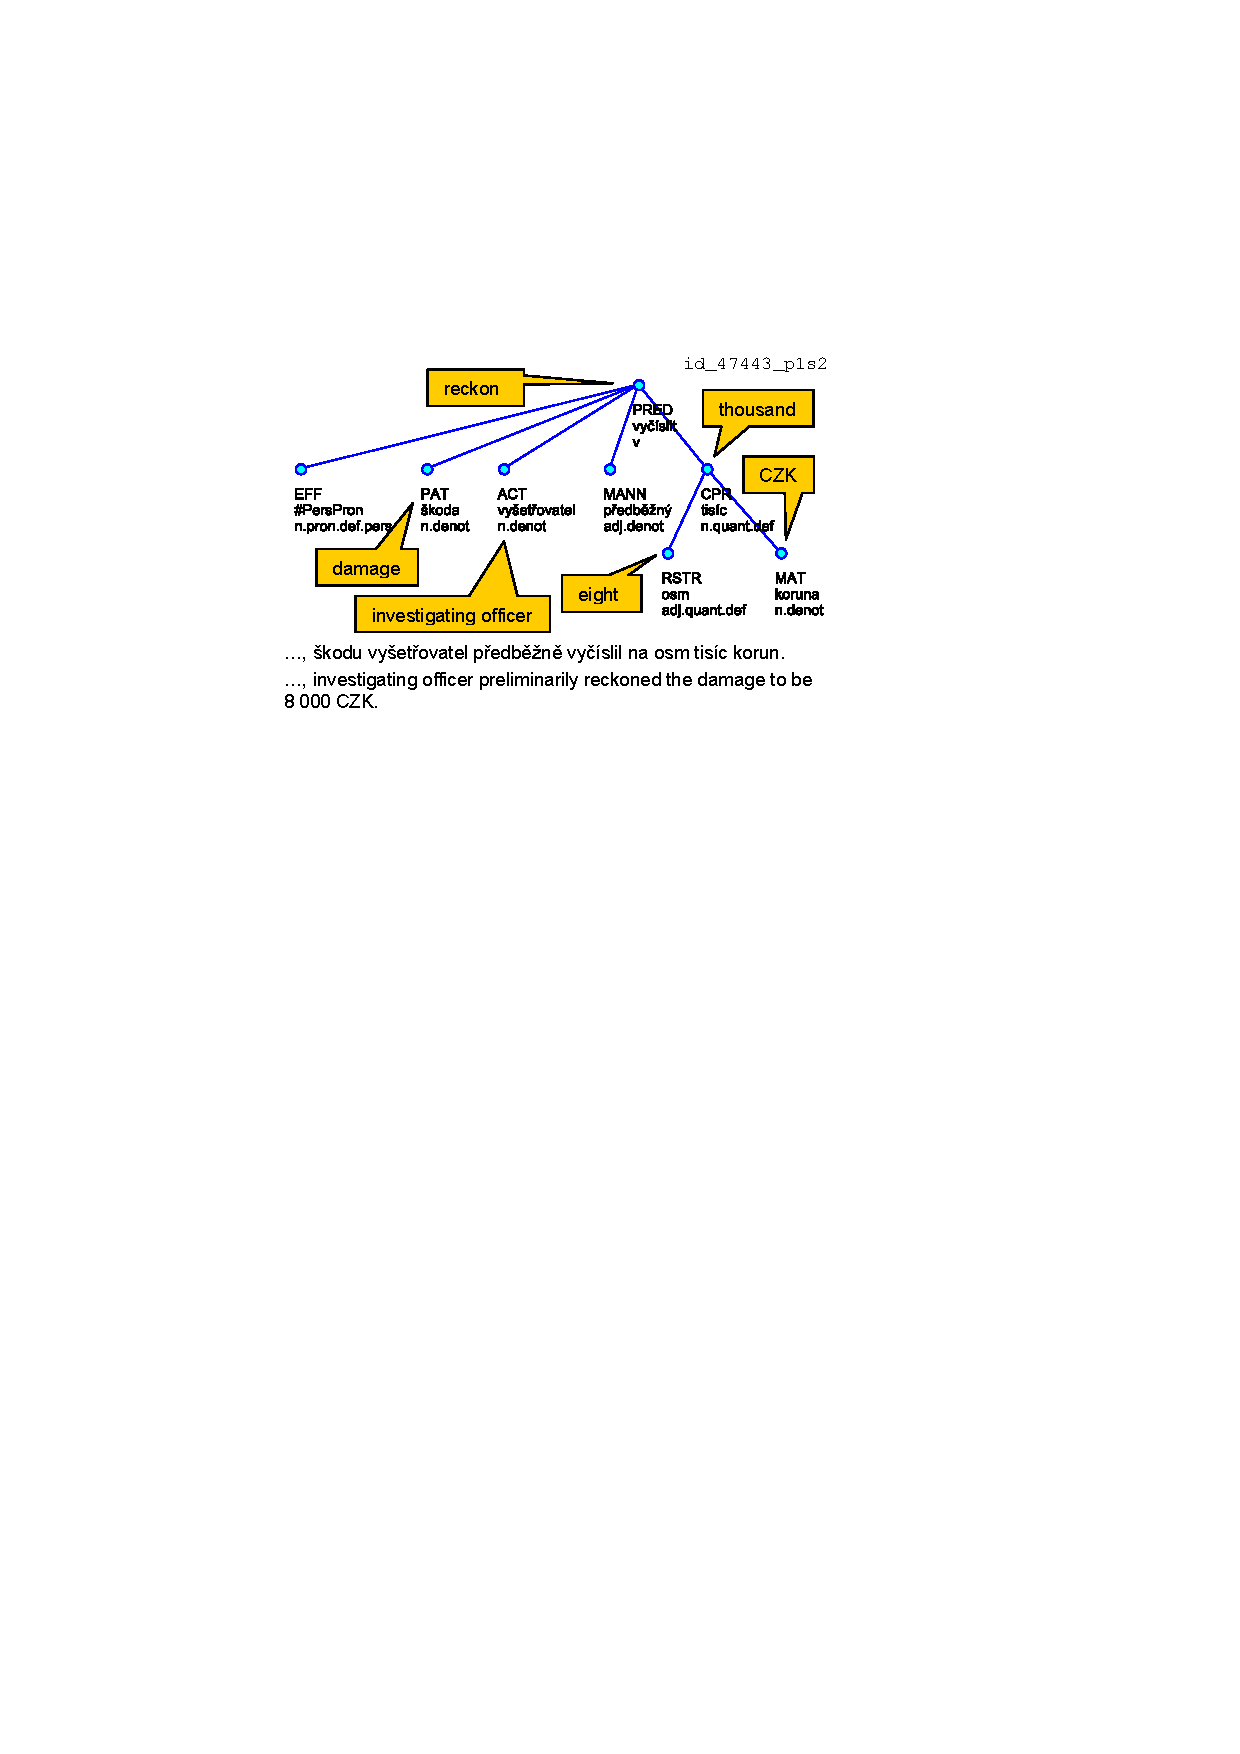
\includegraphics[width=0.55\hsize]{damage_tree}}}
\caption{Example of a linguistic tree of one analyzed sentence.}
\label{fig:intro_damage_tree} 
\end{figure}



\section{Main Goals and Contributions}

To be written!!!

----

The main \emph{contributions} presented in this chapter are \emph{formal models}, prototype \emph{implementation} and experimental \emph{evaluation} of the Fuzzy ILP Classifier.



\section{Organization}

Rather than presenting individual topics or approaches of this thesis separately in distinct chapters, we decided to organize this document according to common aspects of these approaches and to dedicate individual chapters to these aspects instead of individual approaches. This way, all the (four) approaches are described in parallel in each chapter. 

Chapter~\ref{sec:ch_problems} provides definitions of the individual problems and consequent tasks solved in this thesis.

Chapter~\ref{sec:ch_related} contains description of the most related work of other scientists.

Chapter~\ref{sec:ch_third_party} introduces the most important third party tools and resources that were used in our research.

Chapter~\ref{sec:ch_methods} describes solutions, used models and methods if the individual approaches of the present thesis.

Chapter~\ref{sec:ch_implementation} provides details about implementation of all the approaches.

Chapter~\ref{sec:ch_data} describes all datasets that were used in our experiments.

Chapter~\ref{sec:ch_eval} describes all experiments that we performed mostly for evaluation of the approaches.

Chapter~\ref{sec:ch_conclusion} concludes the thesis.


\chapter{Problems and Consequent Tasks Definitions} \label{sec:ch_problems}

As already said in introduction, four separate topics are presented in this thesis. This chapter provides definitions of the main problems connected with these topics and consequent tasks that have to be addressed to solve these problems.

\section{Information Extraction}

\subsection{The Problem}

The basic problem addressed by information extraction approaches can be formulated as follows. We have a large collection of texts (or a source of texts) and we want to have a machine readable (understandable, workable) or structured form of the information present in these texts. Why? Because additional postprocessing of the information is needed.

Let us for example have texts about acquisition events. Each text describes a single acquisition event and you can find answers to following questions in these texts. 

What was the object of the acquisition? 

Who was the buyer? 

What was the deal amount?

What was the acquisition date?

If we put the corresponding information into a relational table then we can easily obtain statistics like numbers of acquisitions per month of the year or a list of ten most valuable (largest deal amount) acquired subjects, etc. This would be impossible if the information were kept in the textual form only.

Document search and indexing is another important purpose of information extraction. Let us imagine a person interested in articles about acquisitions made in January 2009 where the deal amount was between 100 and 500 million dollars.  Keyword search and indexing can not satisfy this need accurately. But if we have corresponding machine readable information, it is easy to create a simple search engine supporting this kind of queries.

The idea of the Semantic Web [citace TBL] brings us to even a bigger problem that could be solved by information extraction approaches. On the Semantic Web, as much information as possible should be in structured machine readable form. But absolute majority of ordinary content of the present day web is understandable only by humans. Machines can use only very limited part of the present day web. This issue is often called “Semantic Web Bottleneck” [citace].

\subsection{Consequent Tasks}

The definition of the problem presented in the previous section was general. We did not specify any particular kind of information to be extracted or target structure for capturing it. This is exactly the point, where different kinds of information extraction approaches differ. Currently, the variety of information extraction approaches is huge. In this thesis, we will focus on a small subset only. 

It was already mentioned in the previous section that the source information is captured in plain text. Let us specify it more precisely: 

We are interested in cases where information is expressed in plain text in natural language. We do not consider additional structural information or formatting instructions that may be potentially available e.g. through HTML or XML tags. 

We are primarily interested in texts consisting of natural language sentences. We do not consider textual fragments, tables, etc.

These two options were selected mainly based on our personal interest and background. This setting is very close to the topic of natural language understanding, very attractive problem since the very establishment of artificial intelligence. 
\footnote{See e.g. in the Wikipedia article Natural language understanding: \url{http://en.wikipedia.org/wiki/Natural_language_understanding#History}}
And this setting is also very common in practice, e.g. in news articles, scientific papers, blog posts, official statements and reports, offers, requests, advertisements, etc. 



After the specification of input format, let us specify the kind of information to be extracted and the target structure for capturing it. Higher complexity of the extracted information makes the task more difficult. The entire complexity of human language is still far beyond the boundary of machine workability. In practice, extraction of very simple facts represented by plain relations already provides significant help. For example only one relation (e.g. “acquisition”) with four arguments (“object”, “buyer”, “deal amount” and “date”) would be sufficient for capturing the information about acquisition events mentioned above. In this thesis, we concentrate on these simple relational facts, not considering any of the wide range of possibilities that the human language offers like expression of tense, causality, modality, general statements with quantifiers, etc.



Stating that we will extract “simple relational facts” is still not precise enough and several well established information extraction tasks conform to this statement. We will describe them in Sections 88-99, but before that, it is necessary to explain how the term “document annotation” will be used in this thesis.

\subsection{Document Annotation}

Document Annotation is a term, which usually refers to the process of putting annotations to a document. In this thesis, the term annotations will always refer to a special kind of annotations used in the GATE framework.  These annotations refer to (usually shorter) segments of text and they provide a label (or annotation type) and arbitrary set of features to each such segment (or simply annotation). Each annotation occupies a continuous portion of text between the beginning and the end of the annotation. These annotations can be easily visualized using colored background in text. Different annotation types are usually decorated with different colors; see Figure 99 for an example. Section 99 provides some technical details about this kind of annotations.

There is a very small difference between the process of document annotation and information extraction. In fact they are equivalent in the case we are describing. Because annotations can be reconstructed from extracted relational facts and relational facts can be reconstructed from annotations. There are only two conditions that have to hold true:

(1) It has to be always possible to determine a portion of text representing any extracted fact.

(2) Each annotation has to keep all its relational arguments as annotation features.

Relation name can be saved as annotation label and vice versa.

\subsection{Entity Recognition}

Entity Recognition or Named Entity Recognition corresponds to the extraction task of identification of significant entities (people, organizations, locations, chemicals, genes, etc.) that are present in text. From the annotation perspective, this is the simplest annotation task: just to mark these entities in text and assign correct labels to them. From the relational perspective, this task corresponds with unary relation extraction.

It can be for example illustrated on following sentence:

“Google just announced that it is acquiring Motorola Mobility.”

There are two entities mentioned in this sentence: Google and Motorola Mobility. Both entities have to be extracted and put into correct unary relations, e.g. “organization(Google)” or “company(Google)” depending on the used vocabulary. Or, in the annotation case, they have to be marked in text and annotated with corresponding label (“organization” or “company”).

\subsection{Relation Extraction}

Relation Extraction is an extraction task that usually comes after entity recognition. When all the significant entities are identified, the task is to connect together those entities that are connected in text and to assign the correct label (relation name) to that connection. Let us again use the example sentence about Google acquiring Motorola. The extracted relation should be connecting the two entities (in the right order) and the label would be something like: “acquiredBy”, “purchasing” or “takingOver” (depending on the system vocabulary; note the dependency between the label and the relation orientation.)

\subsection{Event Extraction}

In literature, Relation Extraction usually refers to binary relations only and Event Extraction is used for relations (events) with more arguments. Individual events have to be correctly indentified in text and arguments have to be assigned to them in proper roles. For example an acquisition event can have roles like purchaser, seller, acquired, dollar amount, etc. We have to extend our running example with Motorola to demonstrate event extraction on it:

Google just announced that it is acquiring Motorola Mobility. The search and online advertising company is buying the company for approximately \$12.5 billion (or \$40 per share), in cash.

In this case, both sentences would be covered by the acquisition event and arguments would be: purchaser(Google), acquired(Motorola Mobility) and dollar\_amount(\$12.5 billion).

\subsection{Instance Resolution}

Instance Resolution further extends entity recognition. It aims at linking a particular entity to its unique representative (or identifier) such that the same entities have always the same identifier and, vice versa, different entities have always different identifiers. Disambiguation is the main task that has to be solved by instance resolution.

It can be illustrated on some ambiguous entity, for example “George Bush”. General entity recognition system just marks the string and assigns a corresponding label (e.g. person, politician or president -- depending on the granularity of the system) to it. In extraction case, such system just puts the string into the corresponding relation. 

Instance resolution is more difficult. Instance resolution system has to select the right representative for that entity -- George W. Bush (junior) or George H. W. Bush (senior) that will be probably both available in the system’s database. Similarly, instance resolution system has to assign the same identifier in cases where for example shortcuts are used, e.g. “George W. Bush” and “G. W. Bush” should be linked to the same identifier.

\subsection{Summary}

The problem of information extraction consists in obtaining machine workable form of information that was previously available in textual form only. We have specified that we are interested only in extraction of simple relational facts and that the extracted facts can be kept either as relational data or they can be of the form of document annotations. Depending on the complexity of extracted information, four basic extraction tasks were defined:

\begin{itemize}
	\item Entity Recognition,
	\item Relation Extraction,
	\item Event Extraction and
	\item Instance Resolution.
\end{itemize}

\section{Machine Learning for Information Extraction}

\subsection{The Problem}

Development of an information extraction system is always, more or less, dependent on a concrete domain and extraction tasks. It is always necessary to adapt the system when it should be used in a new domain with new extraction tasks. The difficulty of such adaptation varies. In some cases the whole system has to be redesigned and reimplemented. Many systems are based on some kind of extraction rules or extraction models and only these rules or models have to be adapted in such case. But still, only highly qualified experts can do such adaptation. These experts have to know the extraction system in detail as well as the domain, target data (texts) and extraction tasks. Such qualification is sometimes (e.g. in biomedical domains) unreachable in one person and difficult cooperation of a domain expert with a system expert is necessary. 

\subsection{Consequent Tasks}

Usage of machine learning techniques can address this problem in such a way that the system is capable to adapt itself. But a learning collection of example texts with gold standard annotations has to be provided. The effort needed to build such collection is still big and demanding, but such gold standard collection is not dependent on any concrete extraction system and expert knowledge related to extraction systems is not needed for its construction. 

Another important purpose of machine learning is that extraction rules or models constructed by machine learning techniques are often more successful than those designed manually.

\section{Extraction Ontologies}

\subsection{The Problem}

Information extraction and automated semantic annotation of text are usually done by complex systems and all these systems use some kind of model that represents the actual task and its solution. The model is usually represented as a set of some kind of extraction rules (e.g., regular expressions), gazetteer lists or it is based on some statistical measurements and probability assertions (classification algorithms like Support Vector Machines (SVM), Maximum Entropy Models, Decision Trees, Hidden Markov Models (HMM), Conditional Random Fields (CRF), etc.)



Before the first usage of an information extraction system, such model is either created by a human designer or it is learned from training dataset. Then, in the actual extraction/annotation process, the model is used as a configuration or as a parameter of the particular extraction/annotation system. These models are usually stored in~proprietary formats and they are accessible only by the corresponding system.



In the environment of the Semantic Web it is essential that information is shareable and some ontology based IE systems keep the model in so called extraction ontologies \cite{DBLP:conf/er/EmbleyTL02}. Extraction ontologies should serve as a wrapper for documents of a narrow domain of interest. When we apply an extraction ontology to a document, the ontology identifies objects and relationships present in the document and it associates them with the corresponding ontology terms and thus wraps the document so that it is understandable in terms of the ontology \cite{DBLP:conf/er/EmbleyTL02}.



In practice the extraction ontologies are usually strongly dependent on a particular extraction/annotation system and cannot be used separately. The strong dependency of an extraction ontology on the corresponding system makes it very difficult to share. When an extraction ontology cannot be used outside the system there is also no need to keep the ontology in a standard ontology format (RDF or OWL).



\subsection{Consequent Tasks}

The cause of the problem is that a particular extraction model can only be used and interpreted by the corresponding extraction tool. If an extraction ontology should be shareable, there has to be a commonly used tool that is able to interpret the extraction model encoded by the extraction ontology. For example Semantic Web reasoners can play the role of commonly used tools that can interpret shareable extraction ontologies.



Although it is probably always possible to encode an extraction model using a standard ontology language, only certain way of encoding makes it possible to interpret such model by a standard reasoner in the same way as if the original extraction tool was used. The difference is in semantics. It is not sufficient to encode just the model's data, it is also necessary to encode the semantics of the model. Only then the reasoner is able to interpret the model in the same way as the original tool. If the process of information extraction or semantic annotation should be performed by an ordinary Semantic Web reasoner then only means of semantic inference are available and the extraction process must be correspondingly semantically described.

\section{Document Classification}

\subsection{The Problem}

Similarly to information extraction, document classification solves a problem when we have a large collection of documents and we do not exactly know what the individual documents are about. Document classification helps in cases when we want to just pick such documents that belong to certain category, e.g. to pick only football news from a general collection of sport news articles. 

\subsection{Consequent Tasks}

The task of document classification can be formulated as follows. Having a textual document and a (usually small) set of target categories, the task is to decide to which category the document belongs. 

In the case of the present thesis, we are especially interested in cases when the set of categories is ordered or, in other words, we can always decide which one of any two categories is higher. This kind of categories is mostly used as rankings and individual categories then correspond to ranking degrees, e.g. ranking of seriousness of a traffic accident, which is used in classification experiments of the present thesis.

\chapter{Related Work} \label{sec:ch_related}

This chapter shortly introduces mostly related work of other researchers. The chapter is split to three main sections. Section~\ref{sec:relwork_doc_classification} is dedicated to information extraction approaches, Section~\ref{sec:relwork_ext_ont} to extraction ontologies and Section~\ref{sec:relwork_doc_classification} to document classification.

\section{Information Extraction Approaches} \label{sec:relwork_ie}

\subsection{Deep Linguistic Parsing and Information Extraction}

\cite{Bunescu:phd} stated: 
\begin{quotation}
The choice of the actual learning algorithm depends on the type of structural information available. For example, deep syntactic information provided by current parsers for new types of corpora such as biomedical text is seldom reliable, since most parsers have been trained on different types of narrative. If reliable syntactic information is lacking, sequences of words around and between the two entities can be used as alternative useful discriminators.	
\end{quotation}
Since that time, the situation has improved and deep linguistic parsing is often used even for biomedical texts (because new biomedical corpora are available for retraining of the parsers; see e.g. in \citep{Buyko:2010:EIA:1870658.1870754}) and  dependency graphs constitute the fundamental data structure for syntactic structuring and subsequent knowledge extraction from natural language documents in many contemporary approaches to information extraction (see details about individual information extraction systems in Section~\ref{sec:rel_deep_IE_systems}). Currently, quite a lot of parsers can be used for generation of these structures from natural language texts. 

Besides the possibility of using different parsers there are also various language dependency representations (LDR) such as the Stanford \citep{stanfordDeps} and CoNLL-X \citep{johansson2007a} dependencies and the Functional Generative Description (FGD) \citep{SgallHajicovaPanevova1986} studied mainly in Prague. All the dependency representations are very similar from the structural point of view; they differ mainly in the number of different dependency kinds they offer. FGD provides also additional node attributes and so called layered approach (see in Section~\ref{sec:ch30_pdt}) and is the only representation available for Czech.


It is also worthy to investigate the impact of usage of different LDRs on the performance of information extraction. \cite{Buyko:2010:EIA:1870658.1870754} compared the impact of different LDRs and parsers in their IE system, namely Stanford and CoNLL-X dependencies and usage of different trimming operations. Their findings are definitely not supporting one choice against another because one representation was better for some tasks and another one for other tasks, see examples in their paper. More important seems to be the quality of used parser.



\subsection{IE Systems Based on Deep Language Parsing} \label{sec:rel_deep_IE_systems}


We describe in this section several information extraction systems based on deep language parsing. The systems differ greatly in the manner of using LDR.

\subsubsection{Rule Based Systems}

There are many systems using hand crafted extraction rules based on LDR. These systems need assistance from a human expert that is able to design the extraction rules manually. The advantage of these systems is that there is no need of learning (or training) data collection. For example \cite{RelEx} used a simple set of rules and the Stanford parser\footurl{http://nlp.stanford.edu/software/lex-parser.shtml} for biomedical relation extraction. Shallow and deep parsers were used by \cite{Yakushiji2001} in combination with mapping rules from linguistic expressions to biomedical events.

\subsubsection{Similarity Based Systems}

Several information extraction systems do some kind of similarity search based on the syntactic structure, e.g.
%[Banko: Open Information Extraction from the Web]
\citep{Etzioni08informationExtraction} and
%[Wang: Recognizing Textual Entailment Using Sentence Similarity based on Dependency Tree Skeletons]
\citep{Wang:SimilarityTreeSkeletons}.

\subsubsection{Biomedical Domain}

The
Stanford format is widely used in the biomedical
domain (e.g., by \cite{MiyaoACL2008}, (\cite{Yakushiji2001}) or
\cite{Clegg2005Evaluating}).



\subsubsection{Classical Machine Learning Systems}

Classical machine learning (ML) approaches rely on the existence of a learning collection. They usually use LDR just for construction of learning features for propositional learners like decision trees, neural networks, support vector machines (SVM), etc. Learning features are selected manually when the system is being adapted to new domain or extraction task. For example in \citep{Bunescu:DependencyPaths}, learning features based on so called dependency paths constructed from LDR are used for relation extraction. Similar approach was used in \citep{Buyko:dependencyGraphs} for biomedical event extraction.


\citep{Yaoyong09a} described machine learning facilities available in GATE. This approach is an example of classical adaptation of propositional learners for information extraction. It should be noted that GATE itself does not provide any prebuilt functions for working with LDR but they can be added as they were in our case (see in Section~\ref{sec:LDR_in_GATE}). This is also the software component (GATE Machine Learning PR) to that we have compared our solution. 
%Our solution is also based on GATE (See next sections.)


\subsubsection{Inductive Systems}

There are also systems using some inductive technique e.g. Inductive Logic Programming (ILP, see also Section~\ref{sec:ch30_ILP}) to induce learning features or extraction rules automatically from learning collection. In these cases it is neither necessary to manually design extraction rules nor select the right learning features. For example \cite{DBLP:conf/ilp/RamakrishnanJBS07} used the dependency parser MINIPAR\footurl{http://webdocs.cs.ualberta.ca/~lindek/minipar.htm} \citep{minipar} and ILP for construction of both:
\begin{enumerate}
	\item learning features for SVM classifier and
	\item plain extraction rules.
\end{enumerate}
They compared the success of the two approaches and discoverd that the extraction model constructed by SVM (based on the induced learning features) was more successful than the plain extraction rules directly constructed by ILP.




\subsection{Inductive Logic Programming and Information Extraction}
There are many users of ILP in the linguistic and information extraction area.
For example in \citep{stasinos:phd} ILP was used for shallow parsing and phonotactics.
Authors of \citep{Junker99learningfor} summarized some basic principles of using ILP for learning from text without any linguistic preprocessing. One of the most related approaches to ours can be found in \citep{aitken02:_learn_infor_extrac_rules}. The authors use ILP for extraction of information about chemical compounds and other concepts related to global warming and they try to express the extracted information in terms of ontology. They use only the part of speech analysis and named entity recognition in the preprocessing step. But their inductive procedure uses also additional domain knowledge for the extraction. In \citep{DBLP:conf/ilp/RamakrishnanJBS07} ILP was used to construct good features for propositional learners like SVM to do information extraction. It was discovered that this approach is a little bit more successful than a direct use of ILP but it is also more complicated. The later two approaches could be also employed in our solution.



\subsection{Semantic Annotation}
Last category of information extraction related work goes in the direction of semantics and ontologies. \cite{Bon04b} described  ontology features in GATE. They can be easily used to populate an ontology with the extracted data. We discus this topic later in Section~\ref{sec:SemanticInterpretation}.



%%%%%%%%%%%%%%%%%%%%%%%%%%%%%%%%%%%%%%%%%%%%%%%%%%%%%%%%%%%%%%%%%%%%%%%%%%%%%%%%%%%%%%%%%%%%%%%%%%%%%%%%%%%%%%
\section{Extraction Ontologies} \label{sec:relwork_ext_ont}
%%%%%%%%%%%%%%%%%%%%%%%%%%%%%%%%%%%%%%%%%%%%%%%%%%%%%%%%%%%%%%%%%%%%%%%%%%%%%%%%%%%%%%%%%%%%%%%%%%%%%%%%%%%%%%

Ontology-based Information Extraction (OBIE) \citep{citeulike:7291004} or Ontology-driven Information Extraction \citep{Yildiz:2007:OMO:1793154.1793216} has recently emerged as a subfield of information extraction. Furthermore, Web Information Extraction \citep{DBLP:journals/tkde/ChangKGS06} is a closely related discipline. Many extraction and annotation tools can be found in the above mentioned surveys (\citep{citeulike:7291004,DBLP:journals/tkde/ChangKGS06}), many of the tools also use an ontology as the output format, but almost all of them store their extraction models in proprietary formats and the models are accessible only by the corresponding tool.

In the literature we have found only two approaches that use extraction ontologies. The former one was published by D. Embley \citep{DBLP:conf/er/EmbleyTL02,Embley:2004:TSU:1012294.1012295}
and the later one -- IE system Ex\footnote{\url{http://eso.vse.cz/~labsky/ex/}} was developped by M. Labsk\'{y} \citep{springerlink:10.1007/978-3-642-01891-6_5}. 
But in both cases the extraction ontologies are dependent on the particular tool and they are kept in XML files with a proprietary structure.


By contrast authors of \citep{citeulike:7291004} (a recent survey of OBIE systems) do not agree with allowing for extraction rules to be a part of an ontology. They use two arguments against that:
\begin{enumerate}
	\item Extraction rules are known to contain errors (because they are never 100\% accurate), and objections can be raised on their inclusion in ontologies in terms of formality and accuracy.

	\item It is hard to argue that linguistic extraction rules should be considered a part of an ontology while information extractors based on other IE techniques (such as SVM, HMM, CRF, etc. classifiers used to identify instances of a class when classification is used as the IE technique) should be kept out of it: all IE techniques perform the same task with comparable effectiveness (generally successful but not 100\% accurate). But the techniques advocated for the inclusion of linguistic rules in ontologies cannot accommodate such IE techniques.
	
The authors then conclude that either all information extractors (that use different IE techniques) should be included in the ontologies or none should be included.
\end{enumerate}



Concerning the first argument, we have to take into account that extraction ontologies are not ordinary ontologies, it should be agreed that they do not contain 100\% accurate knowledge. Also the estimated accuracy of the extraction rules can be saved in the extraction ontology and it can then help potential users to decide how much they will trust the extraction ontology.

Concerning the second argument, we agree that in the case of complex classification based models (SVM, HMM, CRF, etc.) serialization of such model to RDF does not make much sense (cf. the next section). But on the other hand we think that there are cases when shareable extraction ontologies can be useful and in the context of Linked Data\footnote{\url{http://linkeddata.org/}} providing shareable descriptions of information extraction rules may be valuable. It is also possible that new standard ways how to encode such models to an ontology will appear in the future.


%it is not always possible to save an extraction model to an ontology (at least not currently). \subsection{Notes on Ontology Definitions}
This short section briefly reminds main ontology definitions because they are touched and in a sense misused in this chapter. The most widely agreed definitions of an ontology emphasize the shared aspect of ontologies: 
\begin{quote}
An ontology is a formal specification of a shared conceptualization.	\citep{so17864}
\end{quote}

\begin{quote}
An ontology is a formal, explicit specification of a shared conceptualization. \citep{Studer1998161}
\end{quote}

Of course the word `shareable' has different meaning from `shared'. (Something that is shareable is not necessarily shared, but on the other hand something that is shared should be shareable.) We do not think that shareable extraction ontologies will contain shared knowledge about how to extract data from documents in certain domain. This is for example not true for all extraction models artificially learned from a training corpus. Here shareable simply means that the extraction rules can be shared amongst software agents and can be used separately from the original tool. This is the deviation in use of the term `ontology' in the context of extraction ontologies in this chapter (similarly for document ontologies, see in Section~\ref{sec:ch70_doc_ont}).






%%%%%%%%%%%%%%%%%%%%%%%%%%%%%%%%%%%%%%%%%%%%%%%%%%%%%%%%%%%%%%%%%%%%%%%%%%%%%%%%%%%%%%%%%%%%%%%%%
\section{Document Classification} \label{sec:relwork_doc_classification}  \label{sec:ch20_doc_classification}
%%%%%%%%%%%%%%%%%%%%%%%%%%%%%%%%%%%%%%%%%%%%%%%%%%%%%%%%%%%%%%%%%%%%%%%%%%%%%%%%%%%%%%%%%%%%%%%%%

\subsection{General Document Classification}

There are plenty of systems dealing with text mining and text classification. In \citep{biblio:ReYaLiOntoText08} the authors use ontology modeling to enhance text identification. The authors of \citep{biblio:CAP} use preprocessed data from National Automotive Sampling System and test various soft computing methods to model severity of injuries (some hybrid methods showed best performance). Methods of Information Retrieval (IR) are numerous, with extraction mainly based on key word search and similarities. The Connection of IR and text mining techniques with web information retrieval can be found in the chapter ``Opinion Mining'' in the book of Bing Liu \citep{biblio:WebDataMining}. 

\subsection{ML Classification with Monotonicity Constraint}
The Fuzzy ILP Classifier can be seen as an ordinary classifier for data with the monotonicity constraint (the target class attribute has to be monotonizable -- a natural ordering has to exist for the target class attribute). There are several other approaches addressing the classification problems with the monotonicity constraint.

The CART-like algorithm for decision tree construction does not guarantee a resulting monotone tree even on a monotone dataset. The algorithm can be modified \citep{biblio:mon_trees} to provide a monotone tree on the dataset by adding the corner elements of a node with an appropriate class label to the existing data whenever necessary.

An interesting approach is presented in \citep{biblio:mon_transf}: first, the dataset is ``corrected'' to be monotone (a minimal number of target class labels is changed to get a monotone dataset), then a learning algorithm (linear programming boosting in the cited paper) is applied.

Several other approaches to monotone classification have been presented, including instance based learning \citep{biblio:ibl} and rough sets \citep{biblio:rough_sets}.









\chapter{Third Party Tools and Resources} \label{sec:ch_third_party}

\graphicspath{{../img/ch30/}}


In our solution we have exploited several tools and formalisms. These can be divided into two groups: linguistics and (inductive) logic programming. First we describe the linguistic tools and formalisms, the rest will follow.



\section{Prague Dependency Treebank (PDT)} \label{sec:ch30_pdt}
There exist several projects\footnote{Prague Dependency Treebank
 (PDT 1.0, PDT 2.0 \citep{biblio:PDT20_CD}), Prague English Dependency Treebank (PEDT 1.0), Prague Czech-English Dependency Treebank (PCEDT 1.0)} 
closely related to the ``Prague school of dependency linguistics’’ and the Institute of Formal and Applied Linguistics\footnote{\url{http://ufal.mff.cuni.cz}} in Prague, Czech Republic (ÚFAL). All the projects share common methodology and principles concerning the formal representation of natural language %(Czech above all; and recently also English)
 based on the theory of Functional Generative Description (FGD) \citep{SgallHajicovaPanevova1986}. FGD provides a formal framework for natural language representation. It is viewed as a system of layers (stratification) expressing the relations of forms and functions. Special attention is devoted to the layers of language meaning described inter alia in dependency terms.
We will refer to these principles and related formalism as ``PDT principles and formalisms’’ in the present work because the PDT projects are the most fundamental and the elaborate annotation guidelines (see bellow) were compiled within these projects. The most relevant principles for the present work will be briefly described in this section.

\subsection{Layers of Dependency Analysis in PDT}

Unlike the usual approaches to the description of English syntax, the Czech syntactic descriptions are dependency-based, which means that every edge of a syntactic tree captures the relation of dependency between a governor and its dependent node. 

In PDT, text is split into individual sentences and dependency trees are built form them. Nodes of the trees are represented by individual words or tokens and edges represent their linguistic dependencies (simplified speaking, see bellow). Among others, two most important kinds of dependencies are distinguished: syntactical dependencies and ``underlying (deep) structure’’ dependencies. Syntactical dependencies are often called \emph{analytical} and the latter are called \emph{tectogrammatical} dependencies. These two kinds of dependencies form two kinds of dependency trees: \emph{analytical trees} and \emph{tectogrammatical trees}. The situation is usually described using a concept of different layers (or levels) of annotation. It is illustrated by Figure~\ref{fig:ch30_layers}. The description starts at the bottom with the surface structure of a sentence (\emph{w-layer}); note that there is a spelling error -- missing space between words `do’ and `lesa’ (into forest) in the example sentence. The lowest level of linguistic annotation (\emph{m-layer}) represents morphology. Word forms are disambiguated and correct lemmas (dictionary form) and morphological tags are assigned at this level. The second level of annotation is called analytical (\emph{a-layer}). At this level the syntactical dependencies of words are captured (e.g. subject, predicate, object, attribute, adverbial, etc.) The top level of annotation is called tectogrammatical (\emph{t-layer}), sometimes also called ``layer of deep syntax''. At this level some tokens (e.g. tokens without lexical meaning) are leaved out or ``merged’’ together (e.g. prepositions are merged with referred words). Also some nodes without a morphological level counterpart are inserted to the tectogrammatical tree at certain occasions (e.g. a node representing omitted subject -- on Figure~\ref{fig:ch30_layers} labeled as ``\#PersPron’’).  

More over all the layers are interconnected and additional linguistic features are assigned to tree nodes. Among others: \emph{morphological tag} and \emph{lemma} is assigned at the morphological level; \emph{analytical function} (the actual kind of the particular analytical dependency, e.g. predicate, subject, object, etc.) is assigned to dependent nodes at the analytical level; \emph{semantic parts of speech} + \emph{grammatemes} (e.g. \emph{definite quantificational semantic noun} (n.quant.def) + \emph{number} and \emph{gender}, etc.) and \emph{tectogrammatical functor} (e.g. actor (ACT), patient (PAT), addressee (ADDR), temporal: when (TWHEN), directional: to (DIR3), etc.) is assigned at the tectogrammatical level. 

\medskip
Detailed information can be found:
\begin{itemize}
	\item Homepage of the PDT 2.0 project: \url{http://ufal.mff.cuni.cz/pdt2.0/}
	\item Annotation guidelines:	
	\begin{itemize}
		\item Morphological Layer Annotation \citep{mmanCz2005}
		\item Analytical Layer Annotation \citep{amanEn1999}
		\item Tectogrammatical Layer Annotation \citep{biblio:MiBeAnnotationtectogrammatical2006}
		\item Tectogrammatical Layer Annotation for English (PEDT 1.0) \citep{biblio:CiHaAnnotationEnglish2006}
		
	\end{itemize}	
\end{itemize}

\subsection{Why Tectogrammatical Dependencies?}

The practice has shown that representing only syntactical roles of tokens present in a sentence is not sufficient to capture the actual meaning of the sentence. Therefore the tectogrammatical level of representation was established.

Or according to \cite{biblio:KlTransformationBasedTectogrammatical2006}:

\begin{quote}
Annotation of a sentence at this [tectogrammatical] layer is closer to meaning of the sentence than its syntactic annotation and thus information captured at the tectogrammatical layer is crucial for machine understanding of a natural language. This can be used in areas such as machine translation and information retrieval, however it can help other tasks as well, e.g. text synthesis.	
\end{quote}

One particularly important thing about t-layer is that it is designed as unambiguous from the viewpoint of language meaning, which means that synonymous sentences should have the same single representation on t-layer. Obviously this property is very beneficial to information extraction.



\begin{figure}
	\begin{center}
	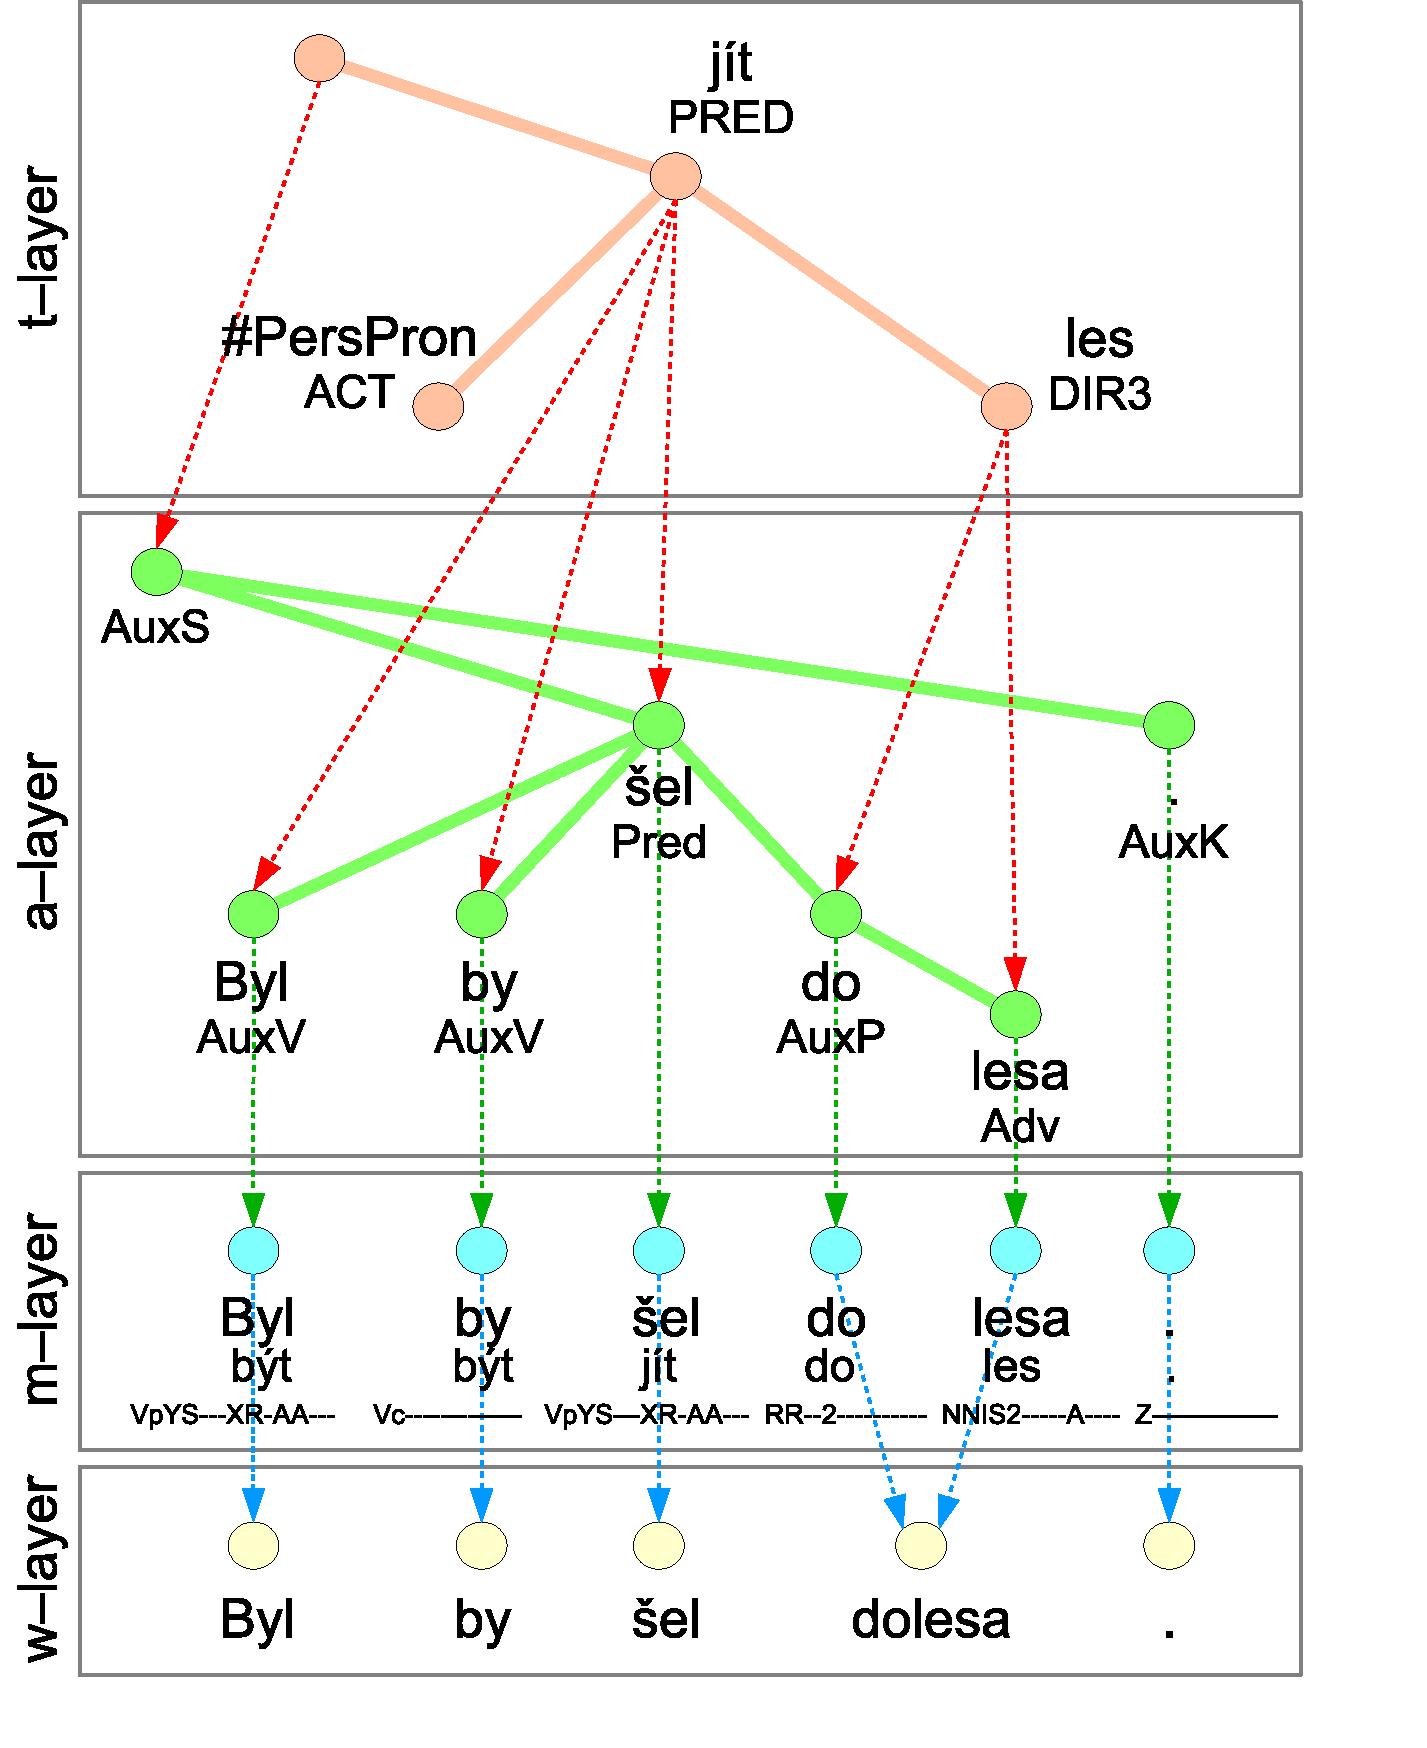
\includegraphics[width=0.6\hsize]{PDT_layers}
		\begin{tabular}{rlllll}
Sample sentence (in Czech): & & Byl & by & šel & dolesa.\\
English translation (lit.):& [He] & would & have & gone & intoforest.			
		\end{tabular}
	\end{center}
\caption{Layers of linguistic annotation in PDT}
\label{fig:ch30_layers}
\end{figure}





\section{PDT Tools and Resources} \label{sec:ch30_pdt_tools_and_resources}

In this section several linguistic tools and resources that are being developed at ÚFAL will be described. These tools and resources are closely connected with the PDT projects and they have been used also in the present work for various purposes.


%%%%%%%%%%%%%%%%%%%%%%%%%%%%%%%%%%%%%%%%%%%%%%%%%%%%%%%%%%%%%%%%%%%%%%%%%%%%%%%%%%%%%%%%%%%%%%%%%
\subsection{Linguistics Analysis} \label{sec:ch30_ling_tools}
%%%%%%%%%%%%%%%%%%%%%%%%%%%%%%%%%%%%%%%%%%%%%%%%%%%%%%%%%%%%%%%%%%%%%%%%%%%%%%%%%%%%%%%%%%%%%%%%%

Linguistic tools that were used for automated (machine) linguistic annotations of texts will be briefly described in this section. These tools are used as a processing chain and at the end of the chain they produce tectogrammatical dependency trees. 


 
\subsubsection{Tokenization and Segmentation} 
On the beginning of text analysis the input text is divided into tokens (words and punctuation); this is called \emph{tokenization}. Sequences of tokens are then (or simultaneously) divided into sentences; this is called \emph{segmentation}. Note that although the task seems quite simple, especially segmentation is not trivial and painful errors occur at this early stage e.g. caused by abbreviations ended by full stop in the middle of a sentence.

There are several tools available for Czech and English. The oldest (Czech) one can be found on the PDT 2.0 CD-ROM \cite{biblio:PDT20_CD} and several choices are provided by TectoMT (see Section~\ref{sec:ch30_tectomt}) and GATE (see Section~\ref{sec:ch30_gate}). The best choice for Czech is probably TextSeg \citep{TextSeg}, which is available through TectoMT.


		
\subsubsection{Morphological Analysis}

Because Czech is a language with rich inflections, morphological analysis (or at least lemmatization) is an important means to success of any NLP task (starting with key word search and indexing.) In PDT morphological analysis is a necessary precondition for analytical analysis (next section).

The task of morphological analysis is for given word form in given context to select the right pair of lemma (dictionary form) and morphological tag. In PDT the tag includes part of speech (POS) and other linguistic categories like gender, number, grammatical case, tense, etc., see morphological annotation guidelines for details.

For Czech two main tools are available: Feature-based tagger\footnote{\url{http://ufal.mff.cuni.cz/tools.html/fbtag.html}} by \cite{biblio:HajicMorfTag} and perceptron-based tagger Morče\footnote{\url{http://ufal.mff.cuni.cz/morce/}} by \cite{biblio:VoMorphologicalTagging2006}. Morče is several years newer and it achieved few points better accuracy on PDT 2.0 (94.04\% vs. 95.12\% see in \citep{Spoustova07b}). Both tools are available through TectoMT, Morče also for English.

\subsubsection{Analytical Analysis}

The task of Analytical analysis is to build up a syntactical dependency tree (analytical tree) from a morphologically analyzed sentence and to assign right kind of dependency (analytical function) to every edge of the tree.


There were experiments with almost all well known parsers on the Czech PDT data\footnote{See details at \url{http://ufal.mff.cuni.cz/czech-parsing/}}. But two of them have proved in practice: Czech adaptation of Collins' parser \citep{biblio:collinshbrt_1999} and Czech adaptation of McDonald's MST parser \citep{Novak:2007:FEM:1776334.1776350}. Again the second tool is few years newer and few points better in accuracy (80.9\% vs. 84.7\% on PDT 2.0\footnotemark[\value{footnote}]). The Collins' parser can be found on the PDT 2.0 CD-ROM and the MST parser is available through TectoMT.

The analytical analysis of English is not very well established because PEDT 1.0\footnote{\url{http://ufal.mff.cuni.cz/pedt/}} contains only tectogrammatical level of annotation and there is no other English treebank for the analytical level. The English analytical analysis is regarded rather as a part of English tectogrammatical analysis; see details in \citep{Klimes:2007:TTD:1776334.1776341}.



%\textbf{Analytical function assignment} \citep{biblio:AlyticAsign} assigns a description (\emph{analytical function}, in linguistic sense) to every edge in the syntactic (dependency) tree.
	
\subsubsection{Tectogrammatical Analysis}

During tectogrammatical analysis analytical trees are transformed to tectogrammatical ones. Merging, omitting and inserting of tree nodes takes place as well as assignment of all the complex linguistic information of the tectogrammatical level (semantic parts of speech, grammatemes, tectogrammatical functors, etc.)

The tectogrammatical analysis can by performed by a variety of TectoMT ``blocks'' (depending on the amount of requested linguistic information, for example only tectogrammatical functors can be assigned.) Better results can be obtained through transformation-based tools developed by Václav Klimeš: \citep{biblio:KlTransformationBasedTectogrammatical2006} for Czech and \citep{Klimes:2007:TTD:1776334.1776341} for English; they are also available thorough TectoMT.


%\begin{table}
%\centering
	%\begin{tabular}{l|l}
		%Name of the tool & Evaluation results (proclaimed by authors) \\[4pt]
		%\hline
	%Segmentation and tokenization & precision(p): 98,0\%, recall(r): 91,4\% \\[4pt]
	%Morphological analysis & 2,5\% unrecognized words\\
	%Morphological tagging & 93,0\% of tags assigned correctly \\[4pt]
	%Collins' parser -- Czech adaptation & 81,6\% dependencies assigned correctly\\
	%Analytical function assignment & precision: 92\% \\[4pt]
	%Tectogrammatical analysis & dependencies p:~90,2\%, r:~87,9\%\\
	%& assignment of f-tags p:~86,5\%, r:~84,3\%\\
	%\end{tabular}
%\caption{Linguistic tools for machine annotation}
%\label{tab:ling_tools}
%\end{table}
%

\subsection{Tree Editor TrEd, Btred} \label{sec:third_tred}

TrEd is the ÚFAL key tool for work with dependency based linguistic annotations. It provides a comfortable GUI for navigation, viewing and editing of linguistic trees at different levels of annotation, for different languages and different treebank schemas. TrEd is implemented in Perl and it is available for a variety of platforms (Windows, Unix, Linux, Mac OS X).

\medskip
Homepage of the project: \url{http://ufal.mff.cuni.cz/~pajas/tred/}


\subsubsection{Btred}
TrEd can be also controlled using a powerful set of Perl macros and there is also a non-interactive version of TrEd called Btred, which allows batch evaluation of user macros on an arbitrary set of annotated documents.

\medskip
Btred/ntred tutorial: \url{http://ufal.mff.cuni.cz/~pajas/tred/bn-tutorial.html}


\subsubsection{PML Tree Query} \label{sec:ch30_pml_tree_query}
PML Tree Query (PML-TQ) \citep{biblio:PaStSystemfor2009} is a TrEd based module for searching through a treebank using a complex tree based query language.

\medskip
Homepage of the project: \url{http://ufal.mff.cuni.cz/~pajas/pmltq/}



\subsection{TectoMT} \label{sec:ch30_tectomt}
%As we have started with our native language -- Czech (a language with rich morphology and free word order), we had to make tools for processing Czech available in GATE. We have implemented a wrapper for the TectoMT system\footnote{\url{http://ufal.mff.cuni.cz/tectomt/}}  to GATE.

TectoMT \citep{biblio:ZaPtTectoMTHighly2008} is a Czech project that contains many linguistic tools for different languages including Czech and English; all the tools are based on the dependency based linguistic theory and formalism of PDT. It is implemented in Perl; highly exploiting TrEd libraries. The recommended platform is Linux. %Windows (not recomended platform for TectoMT)
It is primarily aimed at machine translation but it can also facilitate development of software solutions of other NLP tasks.

We have used a majority of applicable tools from TectoMT (e.g. tokeniser, sentence splitter, morphological, analytical and tectogrammatical analyzers for Czech and English). We have also developed TectoMT wrapper for GATE, which makes it possible to use TectoMT tools inside GATE, see details in Section~\ref{sec:ch60_tectomt_wrapper}.

Similarly to GATE, TectoMT supports building of application pipelines (\emph{scenarios}) composed of so called \emph{blocks} -- processing units responsible for single independent task (like tokenization, parsing, etc.)

\medskip
Homepage of the project: \url{http://ufal.mff.cuni.cz/tectomt/}


\subsection{Netgraph} \label{sec:ch30_netgraph}

Netgraph \citep{biblio:MiNetgraphA2006} is a linguistic tool used for searching through a syntactically annotated corpus of a natural language (corpus of linguistic dependency trees). Besides the searching capabilities it also provides a GUI for viewing of dependency trees. Both of these features were exploited in the present work.

Netgraph implementation is client-server based and a special query language is used for searching. The query language allows putting restrictions on the shape of a tree and on values of attributes of an arbitrary tree node. Besides that nodes of a query can be marked as optional (not necessarily present in a matching tree) and names can be assigned to query nodes. Naming of query nodes then allows putting restrictions based on referenced nodes (Give me all trees where there is a node with two children and both children have the same lemma.) See also Section~\ref{sec:ch50_Netgraph_Based_Extraction_Rules}, it provides additional information about the query language including example Netgraph queries.

Currently Netgraph is replaced by PML Tree Query (see Section~\ref{sec:ch30_pml_tree_query}) and the Netgraph development is ``discontinued''. We use Netgraph in the present work because it is written in Java, the language of what we use. This also made it possible to use Netgraph inside GATE as a handy viewer of dependency trees, see Section~\ref{sec:ch60_GATE_Netgraph}. 

\medskip
Homepage of the project: \url{http://quest.ms.mff.cuni.cz/netgraph/}


\subsection{Annotation Schemas}
\subsubsection{Prague Markup Language (PML)} \label{sec:ch30_pml}
\subsubsection{Feature Structure (FS)} \label{sec:ch30_fs}


\section{Czech WordNet}

The Figure~99 shows, that it would be useful to gather words with similar meanings in our extraction rules. For example, the rule in the Figure~99 contains long disjunctions of similar words (nodes with numbers 1 and 4). These disjunctions could be replaced with some kind of expression telling that we are looking for any word from some semantic category (e.g. human beings). For this purpose we wanted to use the Czech WordNet \citep{biblio:WordNetCZ2004}. 

After we have explored the records of the Czech WordNet (CzWN) related to the domain of our interest (car accidents, etc.) we have decided not to involve CzWN in the extraction process. The reason is that the coverage of the vocabulary of our domain is rather poor and the semantic connections of words are sometimes unfortunately missing. But we can supply the missing information to CzWN or we can build up a new domain-specific word-net based on the ground of CzWN.  

\medskip
Availability: \url{http://catalog.elra.info/product_info.php?products_id=1089}


\section{Other dependency representations} 
\subsection{CoNLL’X dependencies} 
This dependency
tree format was used in the CoNLL’X
Shared Tasks on multi-lingual dependency
parsing \citep{Buchholz2006CoNLLX}. It has been adopted
by most native dependency parsers and was
originally obtained from Penn Treebank (PTB)
trees using constituent-to-dependency conversion\footnote{\url{http://nlp.cs.lth.se/software/treebank_converter/}} \citep{johansson2007a}.


\subsection{Stanford dependencies}

This format was
proposed by \cite{stanfordDeps} for
semantics-sensitive applications using dependency
representations, and can be obtained using
the Stanford tools\footnote{\url{http://nlp.stanford.edu/software/lex-parser.shtml}} from PTB trees. 




\section{GATE} \label{sec:ch30_gate}
GATE \citep{biblio:GATE_ACL2002} is probably the most widely used tool for text processing. In our solution the capabilities of document and annotation management, utility resources for annotation processing, JAPE grammar rules \citep{Cunningham00jape:a}, machine learning facilities and performance evaluation tools are the most helpful features of GATE that we have used.

\medskip
Homepage of the project: \url{http://gate.ac.uk/}

\subsection{GATE Annotations} \label{sec:ch30_gate_annotations}
Contrary to PDT, GATE annotations\footnote{\url{http://gate.ac.uk/userguide/sec:corpora:dags}} are rather simple and minimalistic. They are designed as labeled segments of text. A single annotation is described by its label (\emph{annotation type}) and starting and ending character offset. Each annotation has a unique identifier (integer ID) and an arbitrary set of \emph{features}\footnote{\url{http://gate.ac.uk/userguide/sec:corpora:features}} (name-value pairs) can be assigned to it. 

For example in a sentence ``Hamish Cunningham leads the GATE team.'', ``Hamish Cunningham'' can be annotated with a GATE annotation starting at character 0, ending at character 16, annotation type: ``Person'', with three features: ``firstName=Hamish; surname= Cunningham; gender=male''; because it is the only annotation, the ID would most probably be 0.

Although the GATE annotation approach seems quite simple, very complex structures can be encoded this way (for example an annotation feature can contain a reference to another annotation using its ID), but such usage of GATE annotations is always tricky to some degree and it is always necessary to establish a convention about that. In Section~\ref{sec:ch60_pdt_in_gate} encoding of PDT dependency annotations in GATE will be presented.

\subsection{Machine Learning in GATE} \label{sec:third_gate_ML}

Figure~\ref{img:ExtractionProcessIntro} learning and annotation process in general (ILP version later, Chapter~\ref{ch:ILP_Learning})


\begin{figure}
\centering
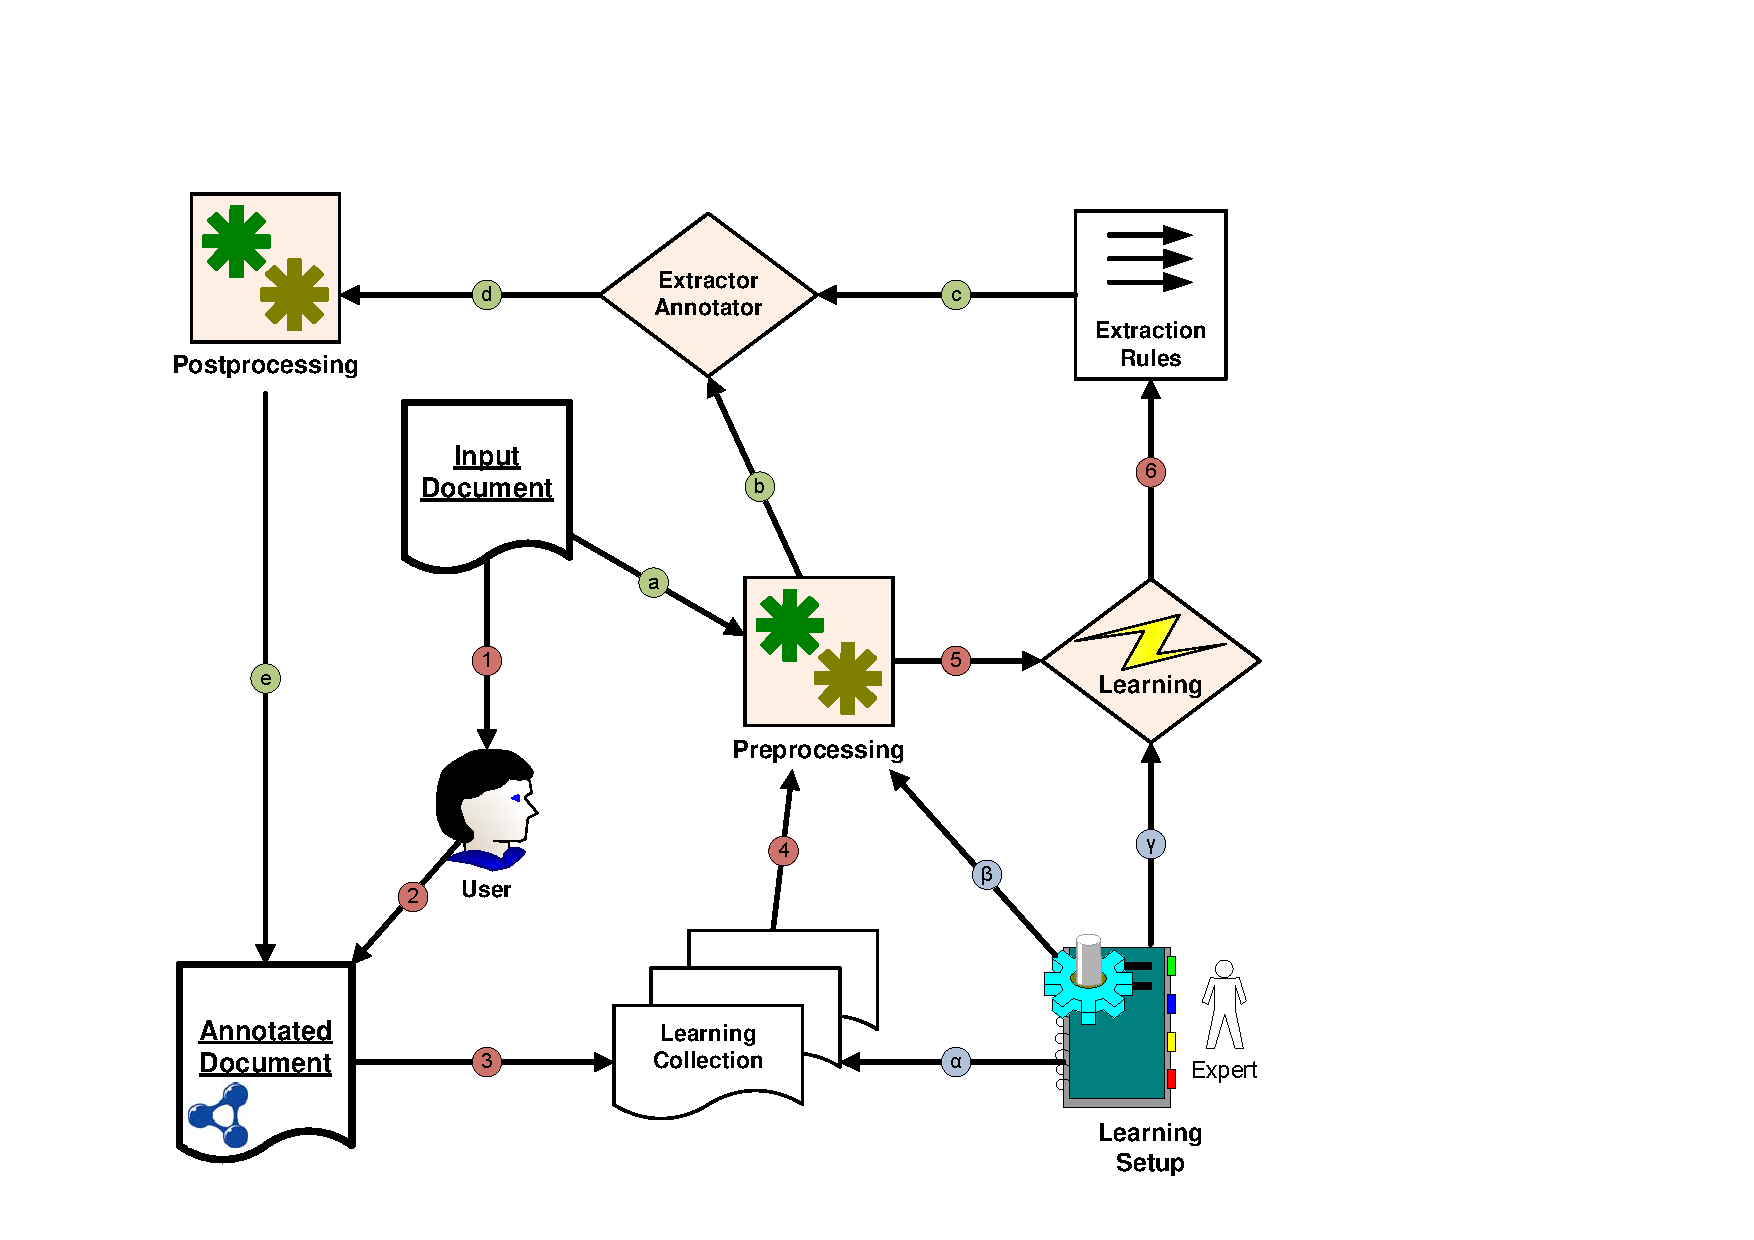
\includegraphics[angle=-90, width=0.8\hsize]{../img/ch10/annotation_process}
\caption{Learning and annotation process -- general overview}
\label{img:ExtractionProcessIntro}
\end{figure}


%%%%%%%%%%%%%%%%%%%%%%%%%%%%%%%%%%%%%%%%%%%%%%%%%%%%%%%%%%%%%%%%%%%%%%%%%%%%%%%%%%%%%%%%%%%%%%%%%
\section{Named Entity Recognition} \label{sec:ch30_named_entity_recognition}
%%%%%%%%%%%%%%%%%%%%%%%%%%%%%%%%%%%%%%%%%%%%%%%%%%%%%%%%%%%%%%%%%%%%%%%%%%%%%%%%%%%%%%%%%%%%%%%%%


%%%%%%%%%%%%%%%%%%%%%%%%%%%%%%%%%%%%%%%%%%%%%%%%%%%%%%%%%%%%%%%%%%%%%%%%%%%%%%%%%%%%%%%%%%%%%%%%%
\section{Inductive Logic Programming} \label{sec:ch30_ILP}
%%%%%%%%%%%%%%%%%%%%%%%%%%%%%%%%%%%%%%%%%%%%%%%%%%%%%%%%%%%%%%%%%%%%%%%%%%%%%%%%%%%%%%%%%%%%%%%%%

Inductive Logic Programming (ILP) \citep{biblio:MuggletonILP} is a machine learning technique based on logic programming. Given an encoding of the known background knowledge (in our case linguistic structure of all sentences) and a set of examples represented as a logical database of facts (in our case tokens annotated with the target annotation type are positive examples and the remaining tokens negative ones), an ILP system will derive a hypothesized logic program (in our case extraction rules) which entails all the positive and none of the negative examples.

Formal definitions of ILP tasks are presented in following sections. They will be extended and used for implementation of Fuzzy ILP Classifier in Chapter~\ref{sec:ch80_fuzzy_ilp_chapter}.






%To make the text easier to read, we present a short description of the ILP techniques below.

%%%%%%%%%%%%%%%%%%%%%%%%%%%%%%%%%%%%%%%%%%%%%%%%%%%%%%%%%%%%%%%%%%%%%%%%%%%%%%%%%%%%%%%%%%%%%%%%%
\subsection{Classical ILP} \label{sec:ch30_ILP_classic}
%%%%%%%%%%%%%%%%%%%%%%%%%%%%%%%%%%%%%%%%%%%%%%%%%%%%%%%%%%%%%%%%%%%%%%%%%%%%%%%%%%%%%%%%%%%%%%%%%

In our presentation of ILP we follow \cite{dzeroski2001:relat_dm} and  \cite{biblio:Muggleton94inductivelogic}.


\theoremstyle{definition}
\newtheorem{definition}{Definition}
\newtheorem{theorem}{Theorem}

\begin{definition}[Classical ILP task]
A set of examples $E=P\cup N$, where $P$ contains positive and $N$ negative examples, and background knowledge denoted by $B$ are given. The task of ILP is to find a hypothesis $H$ such that 

$$
(\forall e\in P)(B\cup H\models e)
$$
and
$$
(\forall e\in N)(B\cup H\not\models e).
$$
\end{definition}
Typically, $E$ consists of ground instances of the target predicate, in our case tree nodes relevant for the praticular extraction task or accident seriousness (see examples in Figure~\ref{img:examples}). $B$ typically consists of several predicates (relational tables), which describe properties of an object, in our case properties of an accident (see examples in Figure~\ref{img:crisp_attributes}) or the structure and properties of linguistic trees. The background knowledge can also contain some rules. A hypothesis $H$ typically consists of logic programming rules (see examples in Figure~\ref{img:rules} and Figure~\ref{fig:rules}). $H$ added to $B$ entails all positive examples and no negative examples.
%
The main advantage of ILP is its multirelational character, namely, $B$ can reside in several relational tables.





%%%%%%%%%%%%%%%%%%%%%%%%%%%%%%%%%%%%%%%%%%%%%%%%%%%%%%%%%%%%%%%%%%%%%%%%%%%%%%%%%%%%%%%%%%%%%%%%%
\subsection{Fuzzy ILP}
%%%%%%%%%%%%%%%%%%%%%%%%%%%%%%%%%%%%%%%%%%%%%%%%%%%%%%%%%%%%%%%%%%%%%%%%%%%%%%%%%%%%%%%%%%%%%%%%%

In our presentation of fuzzy ILP we follow the paper of 
%T. Horv\'ath and P. Vojt\'a\v s 
\cite{biblio:FILP} about fuzzy inductive logic programming.
We use the approach of the fuzzy logic in a narrow sense, developed by 
%J.~Pavelka
\cite{biblio:Pavelka} and 
%P. H\'ajek 
\cite{biblio:Hajek}. Formulas are of the form $\varphi, x$ ($\varphi$ is syntactically the same as in the classical case), they are graded by a truth value $x\in [0,1]$.
A structure ${\mathcal M}$ consists of a domain $M$ and relations are interpreted as fuzzy (we do not consider function symbols here). The evaluation $\left\|\varphi\right\|_{{\mathcal M}}$ of a formula $\varphi$ uses truth functions of many-valued connectives (our logic is extensional and/or truth functional). The satisfaction $\models_f$ is defined by
$$
{\mathcal M}\models_f (\varphi, x)\ iff\ \left\|\varphi\right\|_{{\mathcal M}}\ge x.
$$

\begin{definition}[Fuzzy ILP task]
A fuzzy set of examples ${\mathcal E}:E\longrightarrow [0,1]$ and a fuzzy background knowledge ${\mathcal B}:B\longrightarrow [0,1]$ are given. The task of fuzzy ILP is to find a fuzzy hypothesis ${\mathcal H}:H\longrightarrow [0,1]$ such that 

$$
(\forall e_1,e_2\in E)(\forall {\mathcal M})({\mathcal M}\models_f {\mathcal B}\cup {\mathcal H})
$$
we have
$$
{\mathcal E}(e_1)>{\mathcal E}(e_2)\Rightarrow \left\|e_1\right\|_{{\mathcal M}}\ge \left\|e_2\right\|_{{\mathcal M}}.
$$
That is, it cannot happen that
$$
{\mathcal E}(e_1)>{\mathcal E}(e_2) \wedge \left\|e_1\right\|_{{\mathcal M}}< \left\|e_2\right\|_{{\mathcal M}},
$$
or rephrased: if ${\mathcal E}$ is rating $e_1$ higher than $e_2$, then it cannot happen that $e_1$ is rated worse than $e_2$ in a model of ${\mathcal B}\cup {\mathcal H}$.
\end{definition}

Typically, ${\mathcal E}$ consists of ground instances of the target predicate, which are classified in truth degrees, in case of accident classification, degrees of seriousness of an accident. ${\mathcal B}$ typically consists of several fuzzy predicates (fuzzy relational tables), which describe properties of an object, in our case fuzzy properties of an accident -- a degree of injury, a degree of damage, etc. 
%Background knowledge can contain also some rules, so far only crisp rules are used.
A~hypothesis ${\mathcal H}$ typically consists of a fuzzy logic program, which, when added to ${\mathcal B}$, prevents misclassification (what is better cannot be declared to be worse, nevertheless it can be declared as having the same degree -- for more detailed discussion on this definition of fuzzy ILP we refer to the paper \citep{biblio:FILP}).


\subsection{ILP tool} \label{sec:ch30_ILP_tool}
As an ILP tool we have used ``A Learning Engine for Proposing Hypotheses'' (Aleph v5)\footnote{\url{http://www.comlab.ox.ac.uk/activities/machinelearning/Aleph/}}, which we consider very practical. It uses quite effective method of inverse entailment \citep{biblio:InverseEntailment} and keeps all handy features of a Prolog system (we have used YAP Prolog\footnote{\url{http://www.dcc.fc.up.pt/~vsc/Yap/}}) in its background.


Na rozdil od prologu examples we dvou souborech.

\medskip
Homepage of the project: \url{http://www.comlab.ox.ac.uk/activities/machinelearning/Aleph/}



From our experiments (Section~\ref{sec:evaluation}) can be seen that ILP is capable to find complex and meaningful rules that cover the intended information.



\textbf{?? large amount of training data ??}

As we do not have large amount of training data, there is no problem with excessive time demands during learning and the application of the learned rules is simple and quick.



\section{Weka} \label{sec:ch30_weka}

Weka \citep{biblio:Weka} is a well known data-mining software.

Weka data mining software\footnote{\url{http://www.cs.waikato.ac.nz/ml/weka/}} \citep{biblio:Weka}

Weka Experimenter 

experimenter

usage: evaluation of Fuzzy ILP Classifier (Section~\ref{sec:ch80_eval})

\medskip
Homepage of the project: \url{http://www.cs.waikato.ac.nz/ml/weka/}


\chapter{Models and Methods} \label{sec:ch_methods} 


In this chapter, the four methods corresponding to the four topics of this thesis will be introduced and described. The chapter is structured to four main sections according to the four topics. 



\section{Manual Design of Extraction Rules} \label{sec:manual_methods}
\graphicspath{{../img/ch50/}}

\begin{wrapfigure}[21]{r}{.3\hsize}
\vspace{-0.5cm}
\centerline{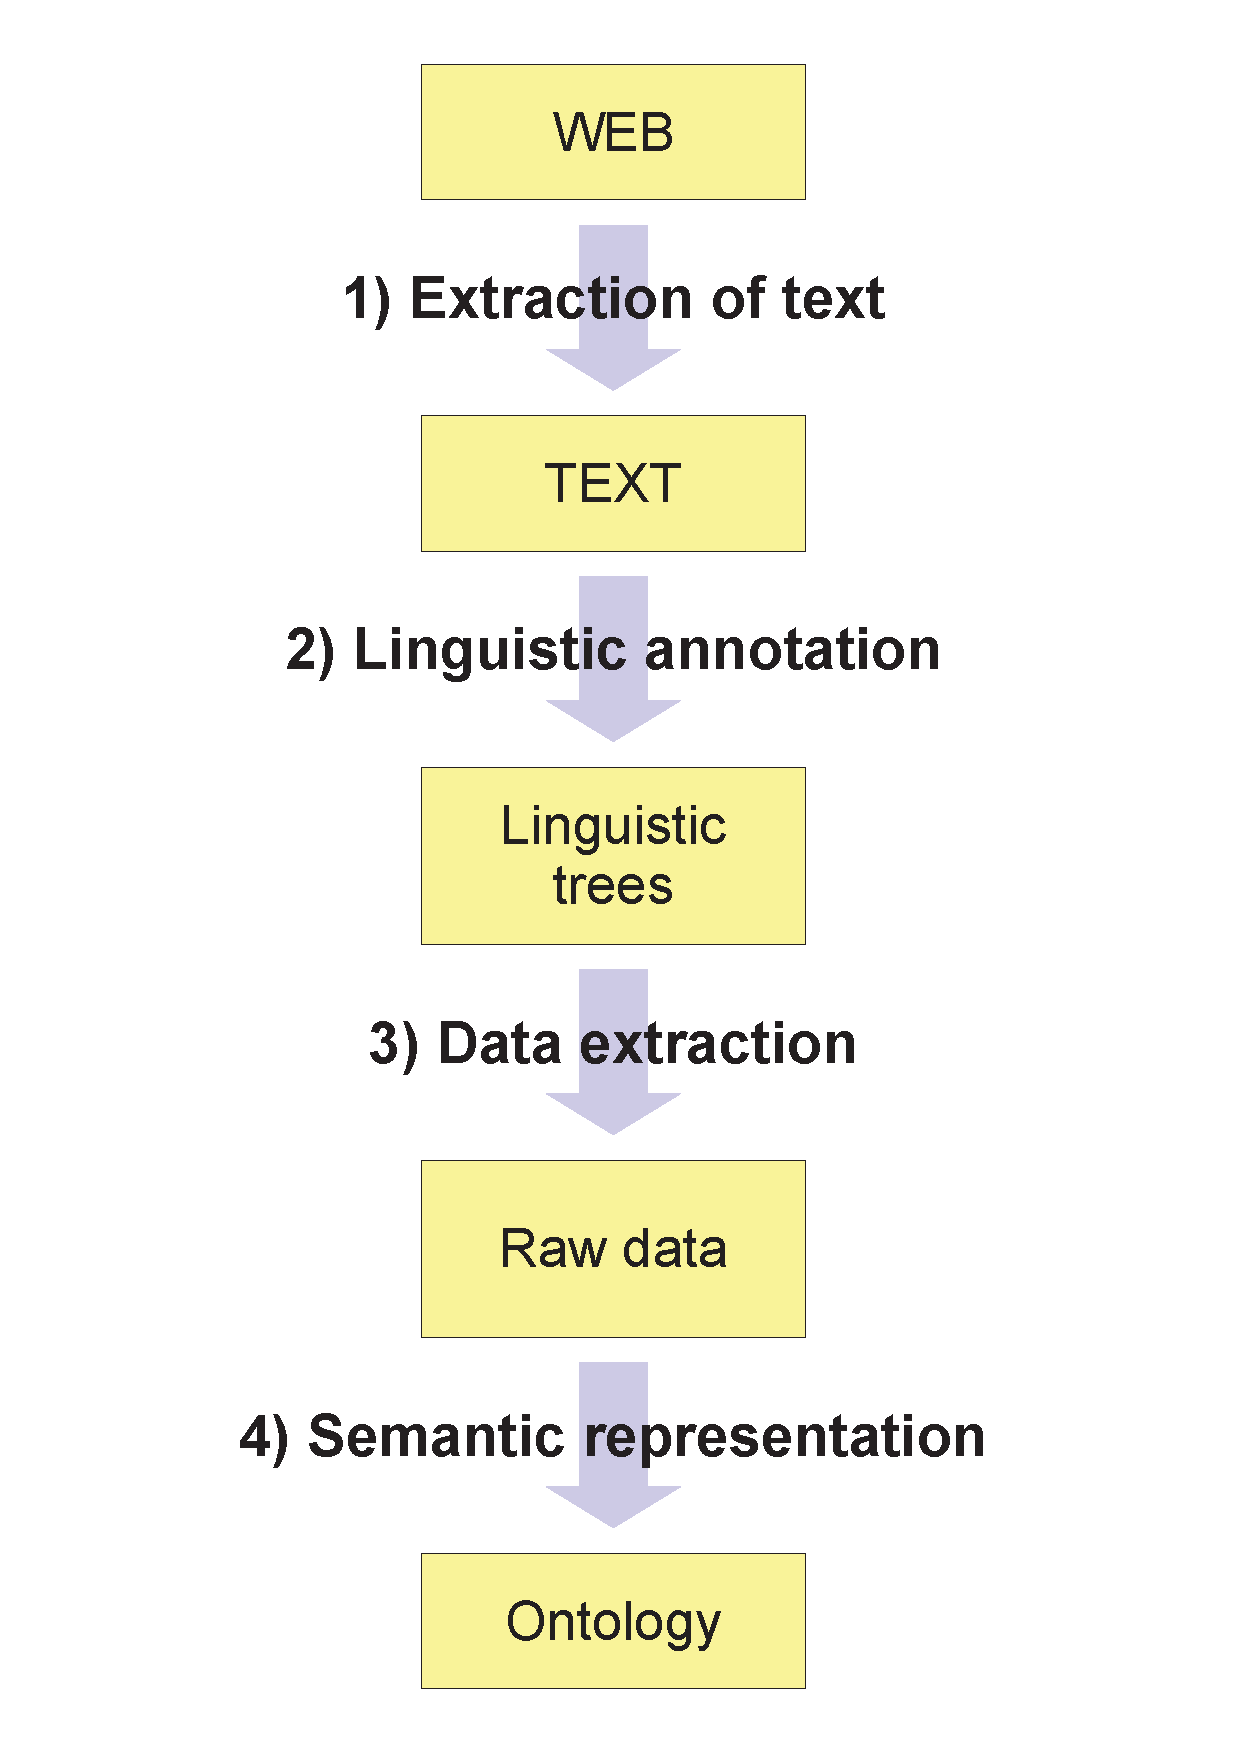
\includegraphics[width=\hsize]{ap_schema}}
\caption{Schema of the extraction process.}
\label{fig:manual_ap_schema}
\end{wrapfigure}

%\begin{figure}
	%\centering
		%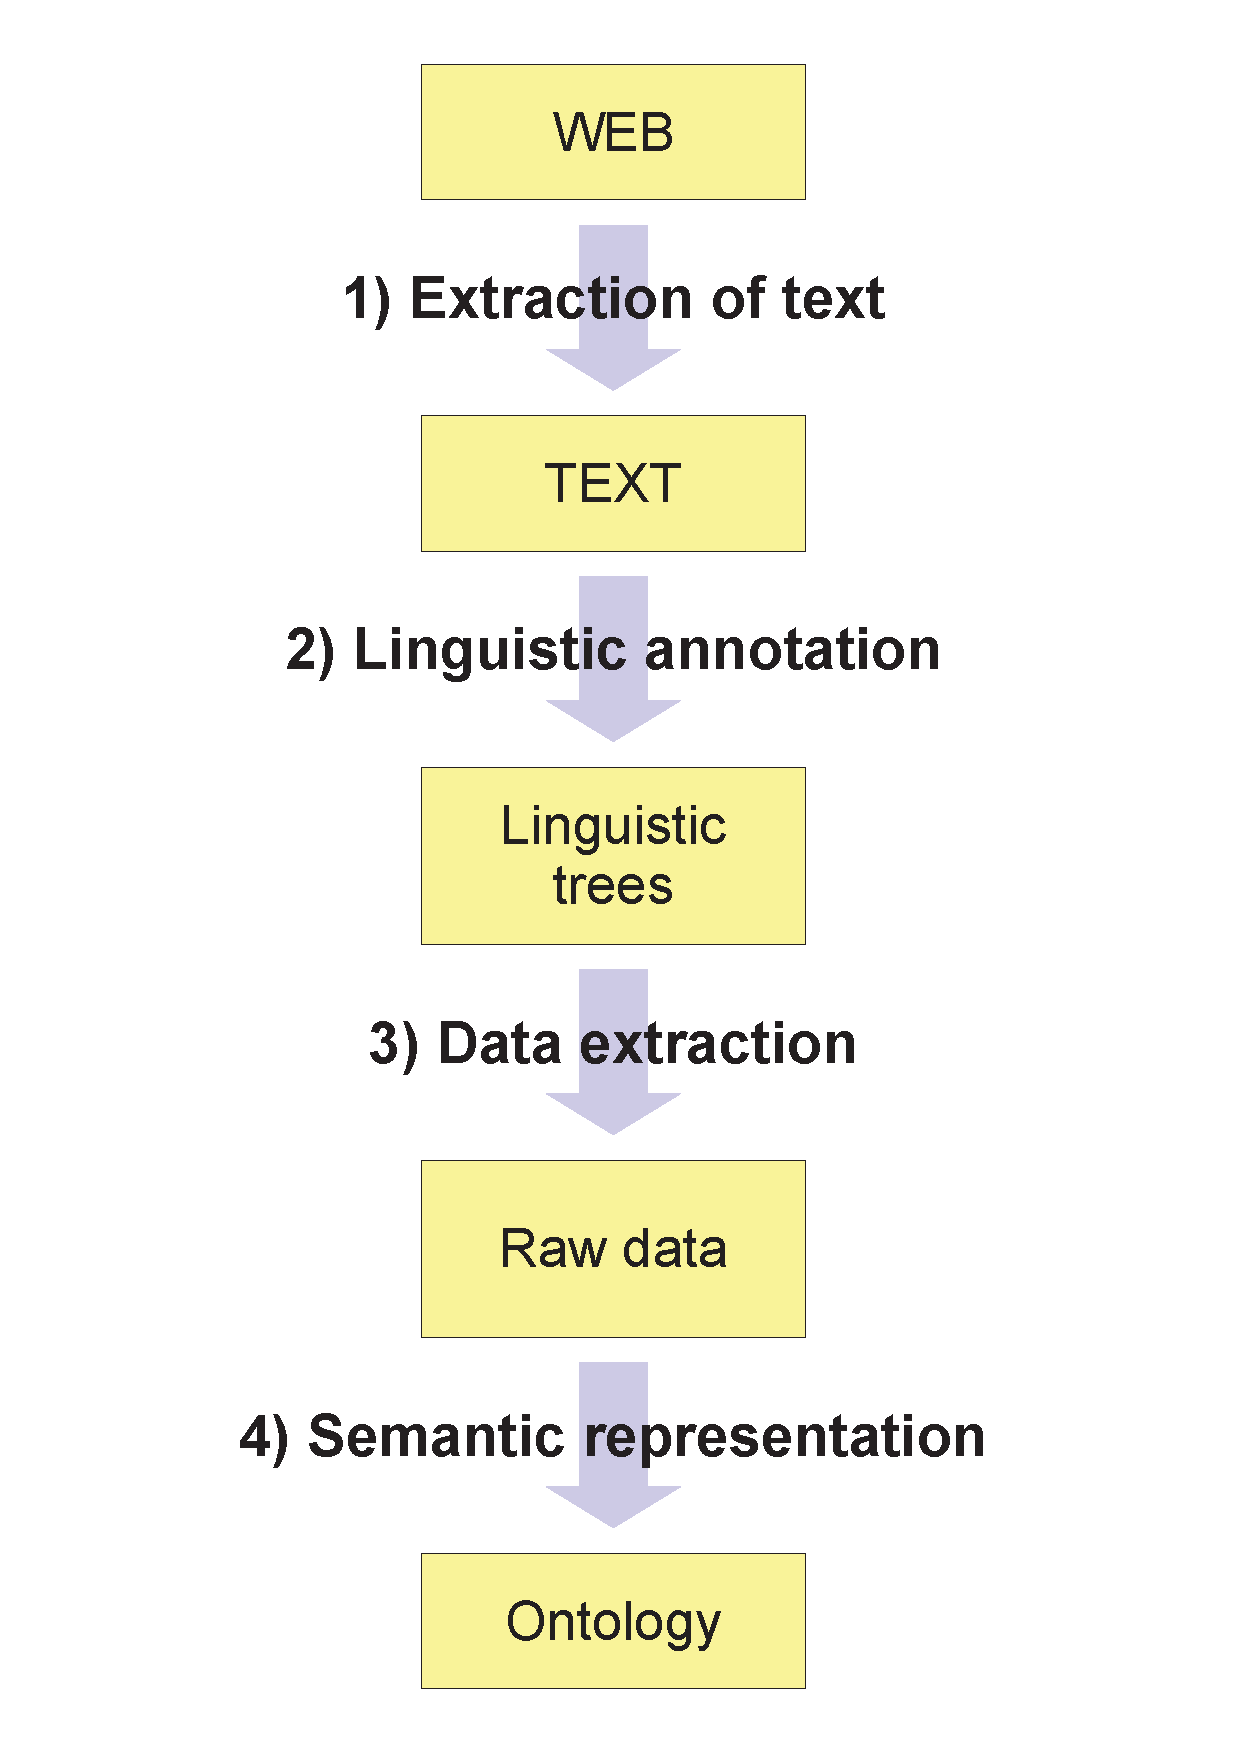
\includegraphics[width=0.2\hsize]{ap_schema}
	%\caption{Schema of the extraction process.}
	%\label{fig:manual_ap_schema}
%\end{figure}


In this section, the extraction method based on manually created linguistic rules will be described. First of all a data flow schema of the extraction process will be presented. Then a description of several stages of evolution of the method will demonstrate how this method came to its existence and which decisions stood behind the development and the final implementation, which will be described in the next chapter.

The approach is based on linguistic preprocessing, oriented to text structured to individual sentences. 



%%%%%%%%%%%%%%%%%%%%%%%%%%%%%%%%%%%%%%%%%%%%%%%%%%%%%%%%%%%%%%%%%%%%%%%%%%%%%%%%%%%%%
\subsection{Data Flow} \label{sec:manual_data_flow}
%%%%%%%%%%%%%%%%%%%%%%%%%%%%%%%%%%%%%%%%%%%%%%%%%%%%%%%%%%%%%%%%%%%%%%%%%%%%%%%%%%%%%





\begin{figure}
	\centering
		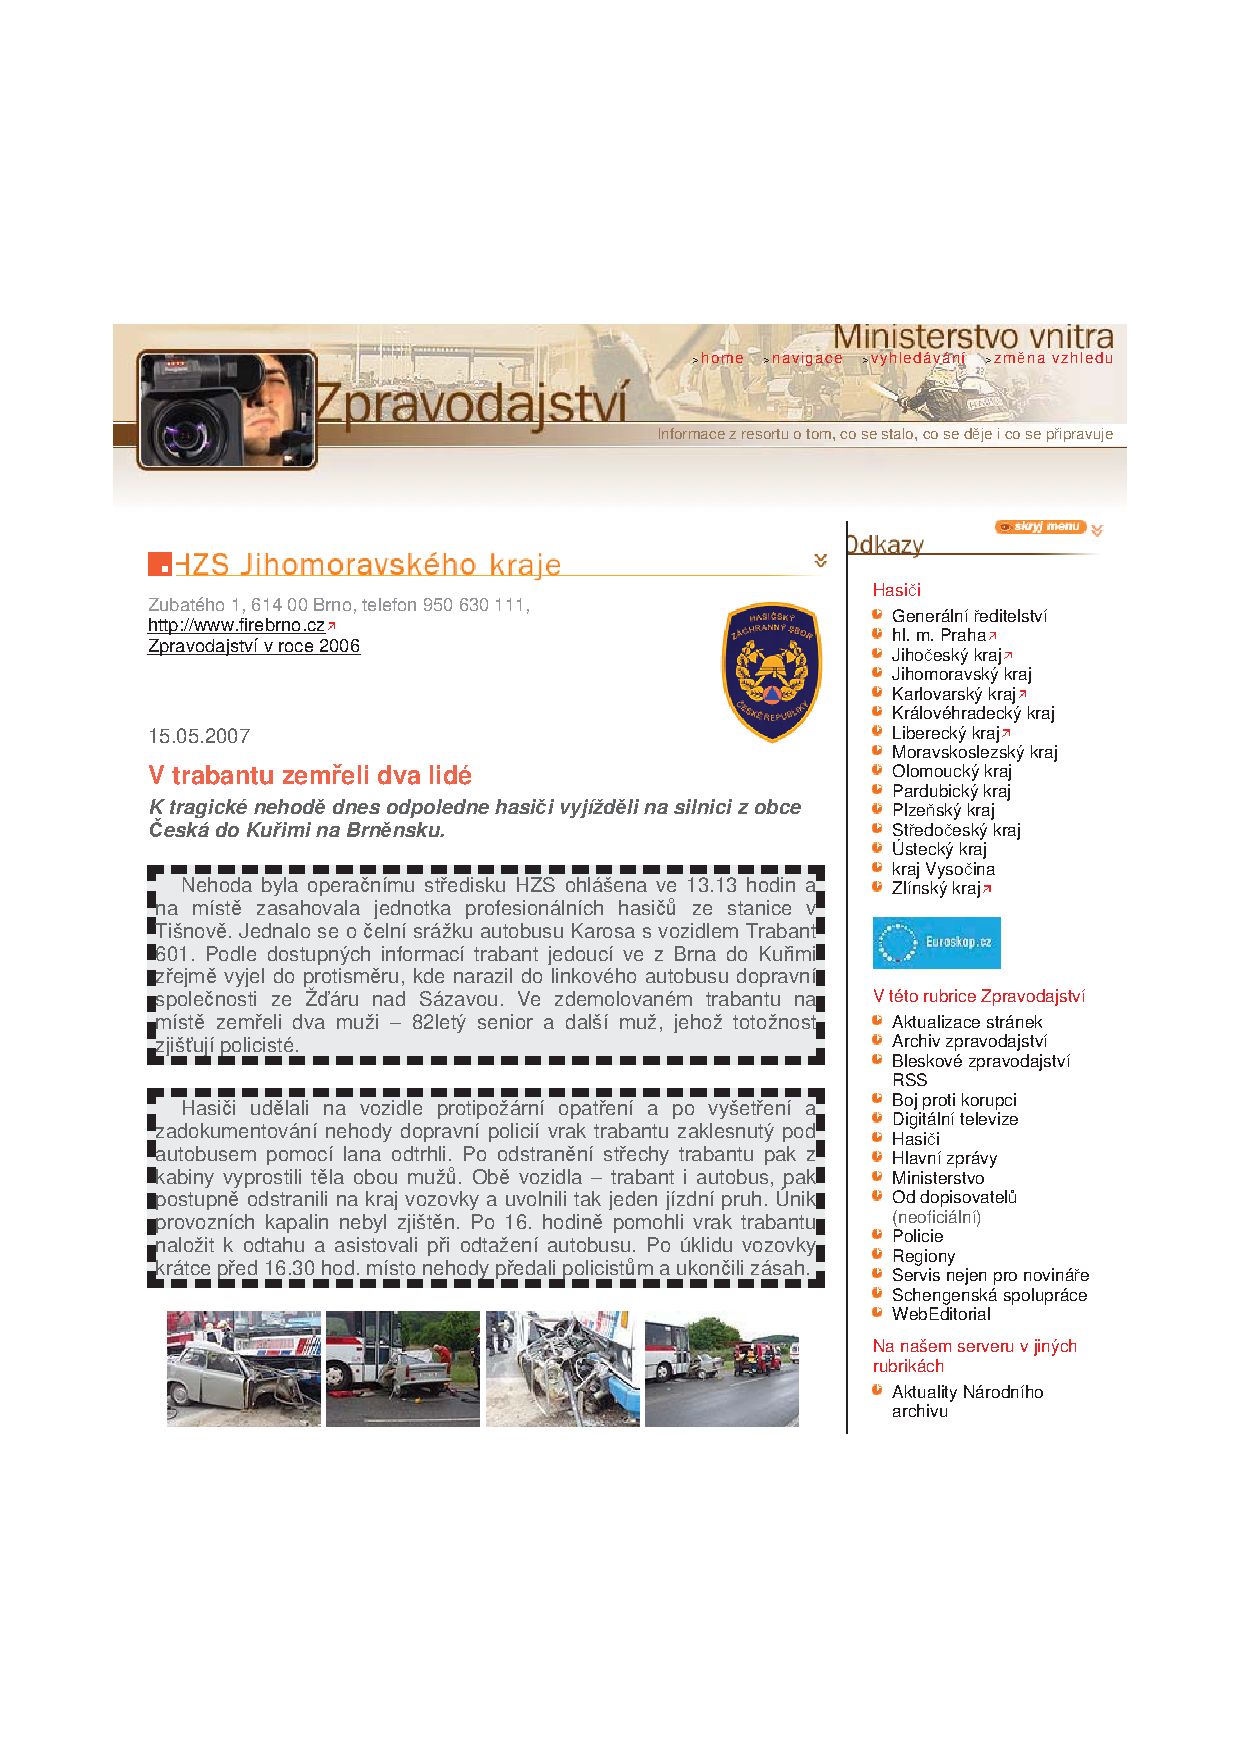
\includegraphics[width=0.7\hsize]{article}
	\caption{One web page with an accident report.}
	\label{fig:manual_article}
\end{figure}


The method was designed as a method for extraction of information from web resources. Thus the extraction process starts on the Web. On the other hand the method was intended to serve the evolution of the Semantic Web, so the final goal of the extraction process is the extracted information stored in the form of a semantic web ontology. A schema in Figure~\ref{fig:manual_ap_schema} splits the process into four steps (phases) among five media types. The schema does not cover the extraction rules design phase; it is assumed that extraction rules were already designed by a human designer; Section~\ref{sec:manual_rules_design} provides details about that. A description of individual steps follows. 



\begin{enumerate}
\item \emph{Extraction of text} \\ First of all, target web pages have to be identified, downloaded and text has to be extracted form them. This issue is not studied in the present work. A RSS feed of the fire department web-site was used to identify and download relevant pages and the desired text (see highlighted area in the Figure~\ref{fig:manual_article}) was extracted by means of a regular expression. The text is an input of the second phase.

\item \emph{Linguistic annotation} \\ In this phase the extracted text is processed by several linguistic tools. The tools analyze the text and produce corresponding set of linguistic dependency trees. There is a rich choice of linguistic tools available (see Section~\ref{sec:third_ling_tools}), but only PDT based tools were used in illustration examples and linguistic trees are always of the form of Tectogrammatical trees, but note that the method is general and it is not limited to the PDT presentation of linguistic dependency trees.

\item \emph{Data extraction} \\ The structure of linguistic dependency trees is used for the extraction of relevant structured data form the text. The extraction method used in this phase is the main topic of this section (Section~\ref{sec:manual_methods}) and details about the method are discuses in following subsections.

\item \emph{Semantic representation} \\ Although the output of the previous phase is already of a structured form, it is not necessarily of the form of a semantic web ontology. The output has to be converted to some ontology format (RDF, OWL) and appropriate schema for given domain and type of extracted information. 

This last step of the extraction process represents a logical distinction between two functionally different tasks of the extraction method. The first task represented by the previous (Data extraction) phase is responsible for choosing of ``what’’ should be extracted, while the second task (Semantic representation) should determine what to do with the extracted data or how to formulate the pieces of information discovered by the Data extraction phase. The border between these two tasks is rather vague and they could be merged together, but we think that the distinction between them can help to understand the problem better.


In the present work only a design of this phase is provided (with a small exception -- using shareable extraction ontologies, see Section~\ref{sec:onto_extraction_ontologies}) because: (1) this task seems to be strongly dependent on manual work of human designers and (2) its potential for meaningful scientific investigation seems to be rather small. Details about this step are further discussed in Section~\ref{sec:manual_sem_interpret}.
\end{enumerate}



%%%%%%%%%%%%%%%%%%%%%%%%%%%%%%%%%%%%%%%%%%%%%%%%%%%%%%%%%%%%%%%%%%%%%%%%%%%%%%%%%%%%%
\subsection{Evolution of the Method}
%%%%%%%%%%%%%%%%%%%%%%%%%%%%%%%%%%%%%%%%%%%%%%%%%%%%%%%%%%%%%%%%%%%%%%%%%%%%%%%%%%%%%

Our first attempt to extract some structured data from linguistically annotated text was done in a standard procedural programming environment (more precisely in Perl, Btred). After an initial phase of development first extraction rule was created as a single executable procedure. This procedure will be described in the next chapter (Section~\ref{sec:manual_Procedural_Extraction_Rules}) and listed in Figure~\ref{fig:btred_rule}. There are many drawbacks of the procedural rule design: such extraction rules are difficult to read, tedious to create, error prone, graphical or assisted design is impossible. On the other hand, this approach has the advantage of the programming language proximity. When a designer designs a procedural extraction rule he or she actually codes it in a procedural programming language and it is easy to add some additional functionality that will be executed and evaluated along with the extraction rule. Thus the designer has the full power of the programming language in hand and he or she can use it inside of the extraction rule. This possibility will be discussed later in the context of semantic interpretation of extracted data.

Dissatisfaction from tedious and time consuming design of procedural extraction rules led us to the idea of a special rule language. We were looking for a language that would allow expressing tree patterns and consequent extraction actions of extraction rules. It turned out that the Netgraph query language is very suitable for the first purpose -- expressing tree patterns. An extension of the Netgraph query language to a language for extraction rules was quite simple then. See the details in the next section.

Last two steps in the evolution of the extraction method were (1) creation of machine learning procedure that is capable to learn extraction rules from manually annotated corpus (see in Section~\ref{sec:learning_methods}) and (2) possibility to export extraction rules to a shareable extraction ontology so the extraction rules can be evaluated on a document by an ordinary semantic web reasoner outside of the original extraction tool (see in Section~\ref{sec:onto_extraction_ontologies}).


%%%%%%%%%%%%%%%%%%%%%%%%%%%%%%%%%%%%%%%%%%%%%%%%%%%%%%%%%%%%%%%%%%%%%%%%%%%%%%%%%%%%%
\subsection{Netgraph Based Extraction Rules}
%%%%%%%%%%%%%%%%%%%%%%%%%%%%%%%%%%%%%%%%%%%%%%%%%%%%%%%%%%%%%%%%%%%%%%%%%%%%%%%%%%%%%

\begin{figure}
	\centering
		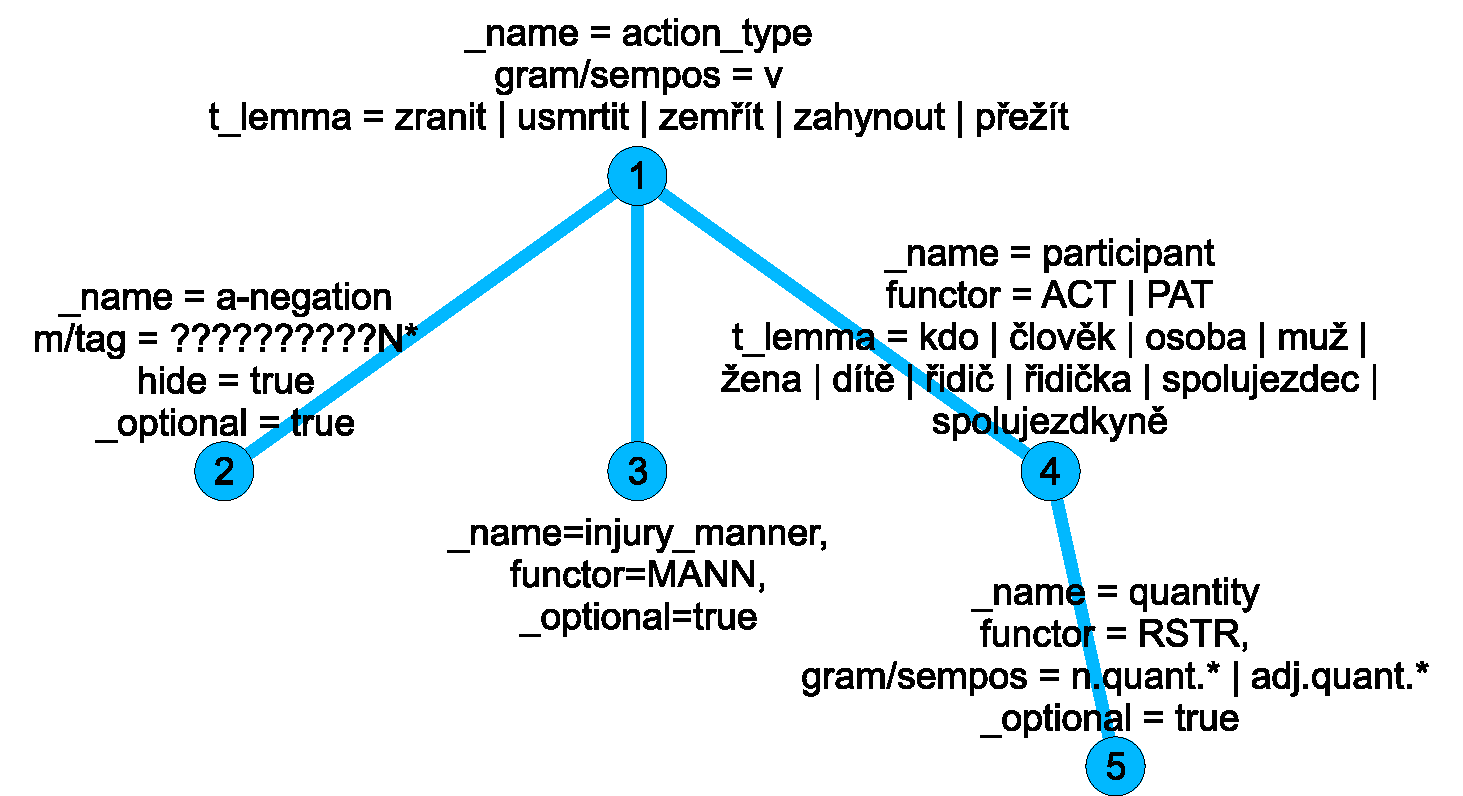
\includegraphics[width=0.5\hsize]{extract_patern}		
\\Transcript:\\
\begin{tabular}{|c|c|c|c|c|}
\hline
zranit & usmrtit & zemřít & zahynout & přežít\\
to injure & to kill & to die & to wane & to survive\\
\hline
\end{tabular}
\\\begin{tabular}{|c|c|c|c|c|c|}
\hline
kdo & člověk & osoba & muž & žena & dítě\\
somebody & (hu)man & person & man & woman & child\\
\hline
\end{tabular}
\\\begin{tabular}{|c|c|c|c|}
\hline
řidič & řidička & spolujezdec & spolujezdkyně\\
driver & woman driver & passenger & woman passenger\\	
\hline
\end{tabular}		
	\caption{A manually created extraction rule investigating numbers of injuries and fatalities.}
	\label{fig:manual_extract_patern}
\end{figure}



Netgraph based extraction rules are declarative, they do not specify a sequential procedure ``what to do with a linguistic tree'', they are rather based on conditions and selections similar to SQL.

Netgraph is a linguistic tool used for searching through a syntactically annotated corpus (see Section~\ref{sec:third_netgraph} for details). Netgraph queries are written in a special query language with a graphical representation. The graphical representation of a query is much better readable than its linear textual representation and we will use the graphical representation only. Figure~\ref{fig:manual_extract_patern} shows an example Netgraph query. It specifies necessary tree structure that has to be present in a matching tree and attribute restrictions that have to hold true for corresponding nodes (the restrictions are printed beside the nodes).



We adopted Netgraph queries and extended them to extraction rules that can be written in following pseudo SQL SELECT form:

\begin{minted}{sql}
SELECT node1_name.attr1_name, node2_name.attr2_name, ... FROM netgraph_query
\end{minted}

where \emph{netgraph\_query} stands for an arbitrary Netgraph query, \emph{node1\_name}, \emph{node2\_name}, etc. stand for individual names of nodes defined in \emph{netgraph\_query} and \emph{attr1\_name}, \emph{attr2\_name}, etc. stand for names of linguistic attributes whose values should be picked out from the corresponding matching tree nodes.

The extraction works as follows: the Netgraph query is evaluated by searching through a corpus of linguistic trees. Matching trees are returned and the desired information defined by the SELECT part of the extraction rule is taken from particular tree nodes and printed to the output.

Let us explain the extraction procedure in detail, using the example of extraction rule from the Figure~\ref{fig:manual_extract_patern}, which is looking for information about killed and injured people during a (usually car) accident. This rule consists of five nodes. Each node of the rule will match with the corresponding node in each matching tree. So we can investigate the relevant information by reading values of linguistic attributes of matching nodes. We can find out the number (node number 5) and kind (4) of people, which were or were not (2) killed or injured (1) by an accident that is presented in the given sentence. And we can also identify the manner of injury (light or heavy) in the node number 3.

Implementation details and some additional examples of these extraction rules will be presented in the next chapter (Section~\ref{sec:manual_impl_rules}).



%%%%%%%%%%%%%%%%%%%%%%%%%%%%%%%%%%%%%%%%%%%%%%%%%%%%%%%%%%%%%%%%%%%%%%%%%%%%%%%%%%%%%
\subsection{Methodology for Rule Designers} \label{sec:manual_rules_design}
%%%%%%%%%%%%%%%%%%%%%%%%%%%%%%%%%%%%%%%%%%%%%%%%%%%%%%%%%%%%%%%%%%%%%%%%%%%%%%%%%%%%%

\begin{figure}
	\centering
		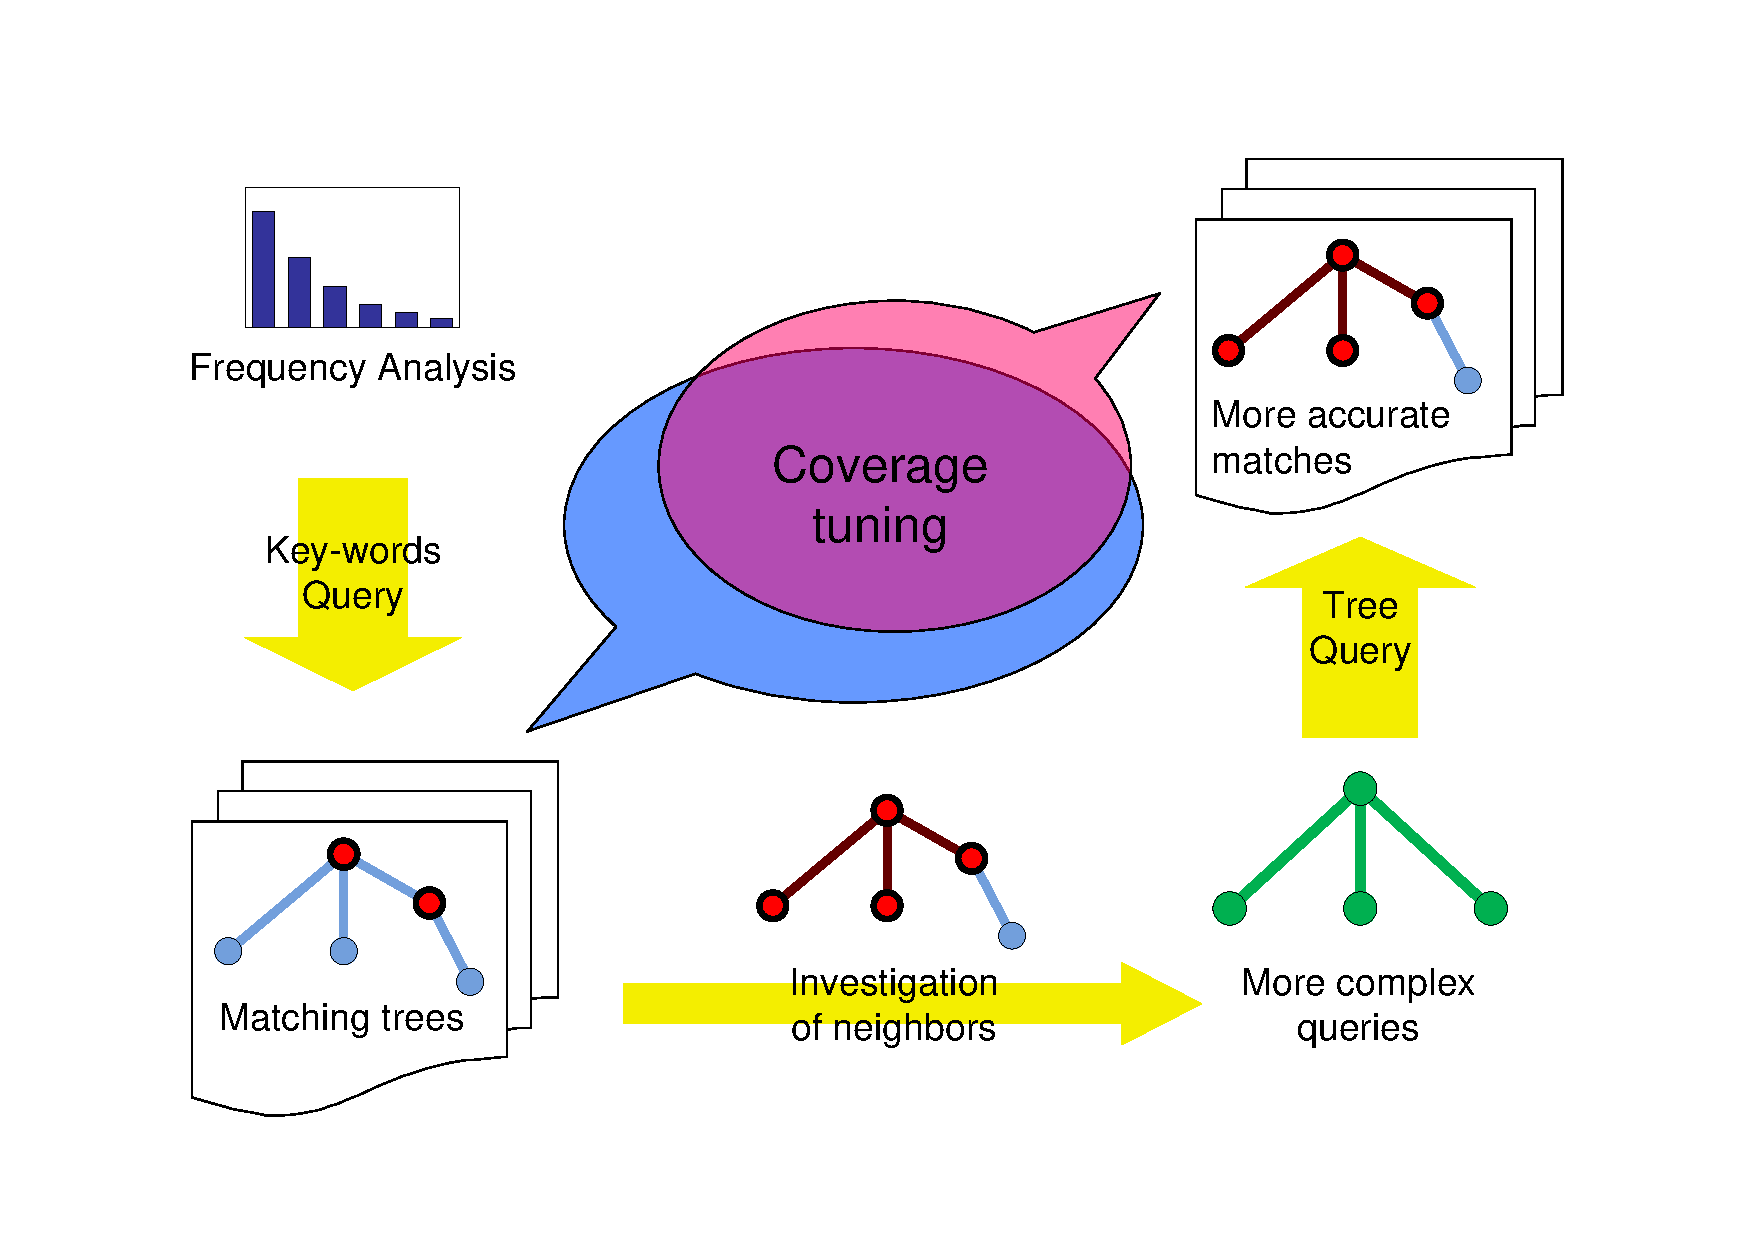
\includegraphics[angle=-90, width=0.5\hsize]{coverge_tuning}
	\caption{Gradual refinement of an extraction rule.}
	\label{fig:manual_coverge_tuning}
\end{figure}


The process of manual design of extraction rules is heavily dependent on skills and experience of a human designer and fulfillment of the process is quite creative task. In this section we try to pick it up as precisely as possible because we assume that a formal description of this process can help in two ways. First -- a new designer can use it as a cook book and progress more quickly. Second -- it can help with development of tools for assisted rule design. We will concentrate on the Netgraph based extraction rules because we think they are more useful.

The process consists of two parts: construction of a Netgraph query and semantic interpretation of the query. The semantic interpretation part will be discussed in the next section.

One obvious preposition of the procedure is that we have a collection of training texts.
The procedure is demonstrated in Figure~\ref{fig:manual_coverge_tuning} and it starts with frequency analysis of words (their lemmas) occurring in the texts. Especially frequency analysis of verbs is very useful --- meaning of a clause is usually strongly dependent on the meaning of the corresponding verb.

\textbf{Frequency analysis} helps the designer to choose some representative words (\textbf{key-words}) that will be further used for searching the training text collection. Ideal choice of key-words would cover the majority of sentences that express the information we are looking for and it should cover minimal number of the not-intended sentences. An initial choice need not be always sufficient and the process could iterate.

Next step of the procedure consists in \textbf{investigating trees} that are covered by key-words. The designer is examining \textbf{matching trees} --- looking for positions of key-words and their \textbf{neighboring} nodes.

After that the designer can formulate an initial \textbf{Netgraph query} and he or she can compare result of the Netgraph query with the coverage of key-words. Based on this he or she can reformulate the query and gradually refine the query and \textbf{tune the query coverage}.

There are two goals of the query tuning. The first goal is maximization of the relevance of the query. An ideal result is a query that covers all sentences expressing given type of information and no other. The second goal is to involve all important tree-nodes to the query. The second goal is important because the \textbf{complexity of the query} (number of involved nodes) makes it possible to extract more complex information. For example see the query on the Figure~\ref{fig:manual_extract_patern} --- each node keeps different kind of information.


%%%%%%%%%%%%%%%%%%%%%%%%%%%%%%%%%%%%%%%%%%%%%%%%%%%%%%%%%%%%%%%%%%%%%%%%%%%%%%%%%%%%%
\subsection{Semantic Interpretation of Extracted Data} \label{sec:manual_sem_interpret}
%%%%%%%%%%%%%%%%%%%%%%%%%%%%%%%%%%%%%%%%%%%%%%%%%%%%%%%%%%%%%%%%%%%%%%%%%%%%%%%%%%%%%

After the designer has successfully formulated the Netgraph query he or she has to supply semantic interpretation of the query. This interpretation expresses how to transform matching nodes of the query (and the available linguistic information connected with the nodes) to the output data.

We did not talk about the extraction output so far. It will be described in the next chapter. For the current description, it is sufficient to say that both methods (the procedural one and the declarative one) have, although structured but still, proprietary XML extraction output. This corresponds to the penultimate stage (raw data) of our data flow schema presented in Section~\ref{sec:manual_data_flow}. In this section, we will describe details about the last step of the data flow schema -- semantic representation of extracted data.

In Section~\ref{sec:manual_impl_output}, the difference between the output of the procedural extraction rule (Section~\ref{sec:manual_Procedural_Extraction_Rules}, Figure~\ref{fig:btred_xml}) and the Netgraph based extraction rule (Section~\ref{sec:manual_Netgraph_Based_Extraction_Rules}, Figure~\ref{fig:select_xml}) can be observed. The procedural one is closer to the semantics of the extracted data while the Netgraph based one is more general, rather based on the semantics of the matching tree and extraction rule. The difference is connected with the difference of the design processes of these extraction rules. While Netgraph based rules are designed in a comfortable way using a graphical tool, the procedural rules have to be coded manually in the programming language of Perl. A Perl programmer has great freedom in the design of a procedural rule and he or she can adapt the rule such that it precisely respects the semantics of extracted data. A designer of a Netgraph based rule has the only freedom in the construction of a Netgraph query and in selection particular query nodes and linguistic attributes that will be selected for the output.

As stated in Section~\ref{sec:manual_data_flow} about the data flow, the goal of our extraction process is in the form of a semantic web ontology. This is not difficult in the case of procedural rules. Once the schema (or vocabulary) of the target ontology is selected, the extraction rules can be simply designed to produce the output of that form (Note that semantic web ontologies can be captured in a specific XML format.)

In the case of Netgraph based queries the situation is more complex and different solutions can be discovered. All the solutions have one thing in common: additional manual work is necessary. The problem is basically to create a mapping of the data in one format (results of Netgraph based rules) to another format (target ontology). It can be done by a variety of technical means (coded in an arbitrary programming language, XSLT, or using a graphical mapping tool like 
Altova MapForce\footnote{\url{http://www.altova.com/mapforce/xml-mapping.html}}
or
Stylus Studio\footnote{\url{http://www.stylusstudio.com/xsd_to_xsd.html}}
). 



\begin{figure}
	\centering
		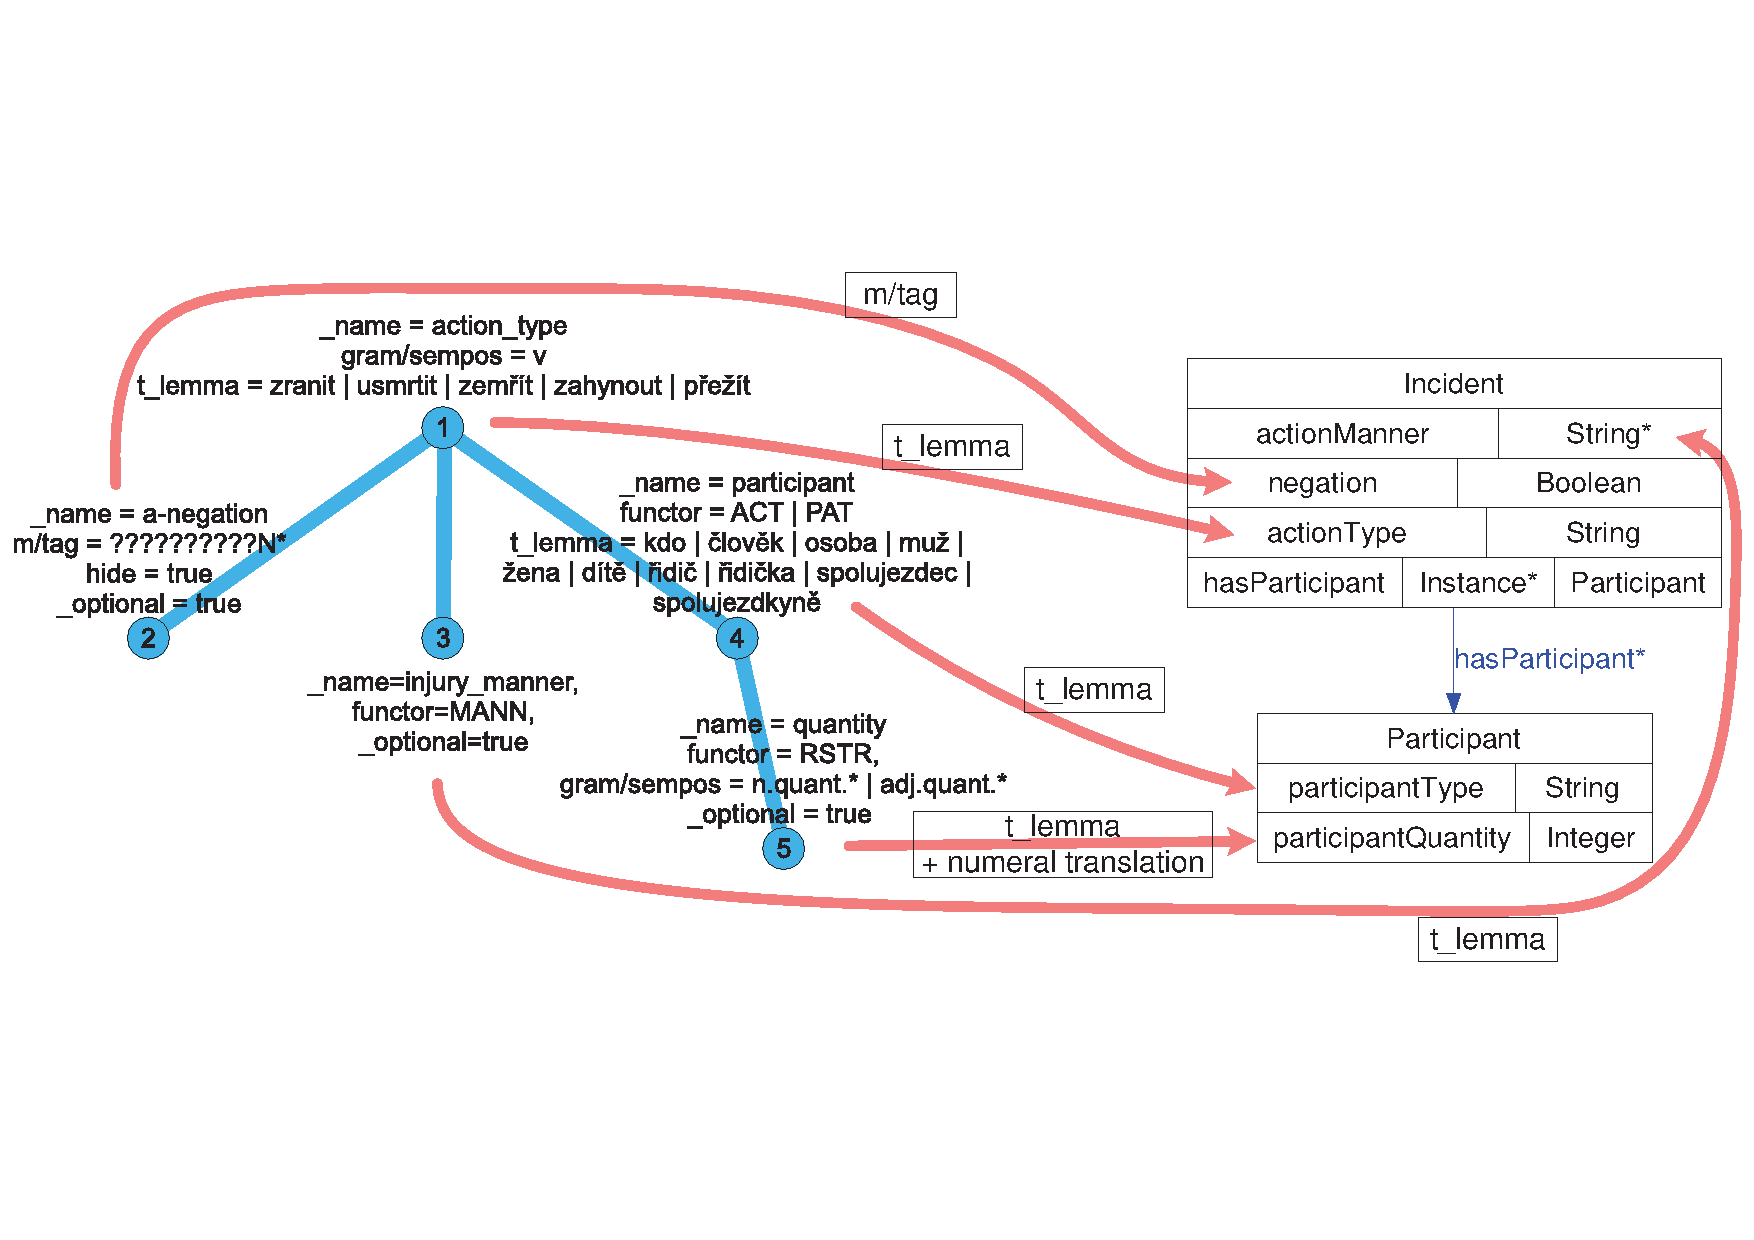
\includegraphics[angle=-90, width=0.9\hsize]{semantic_interpretation}
	\caption{Semantic interpretation of the extraction rule.}
	\label{fig:manual_semantic_interpretation}
\end{figure}


\begin{figure}
	\centering
		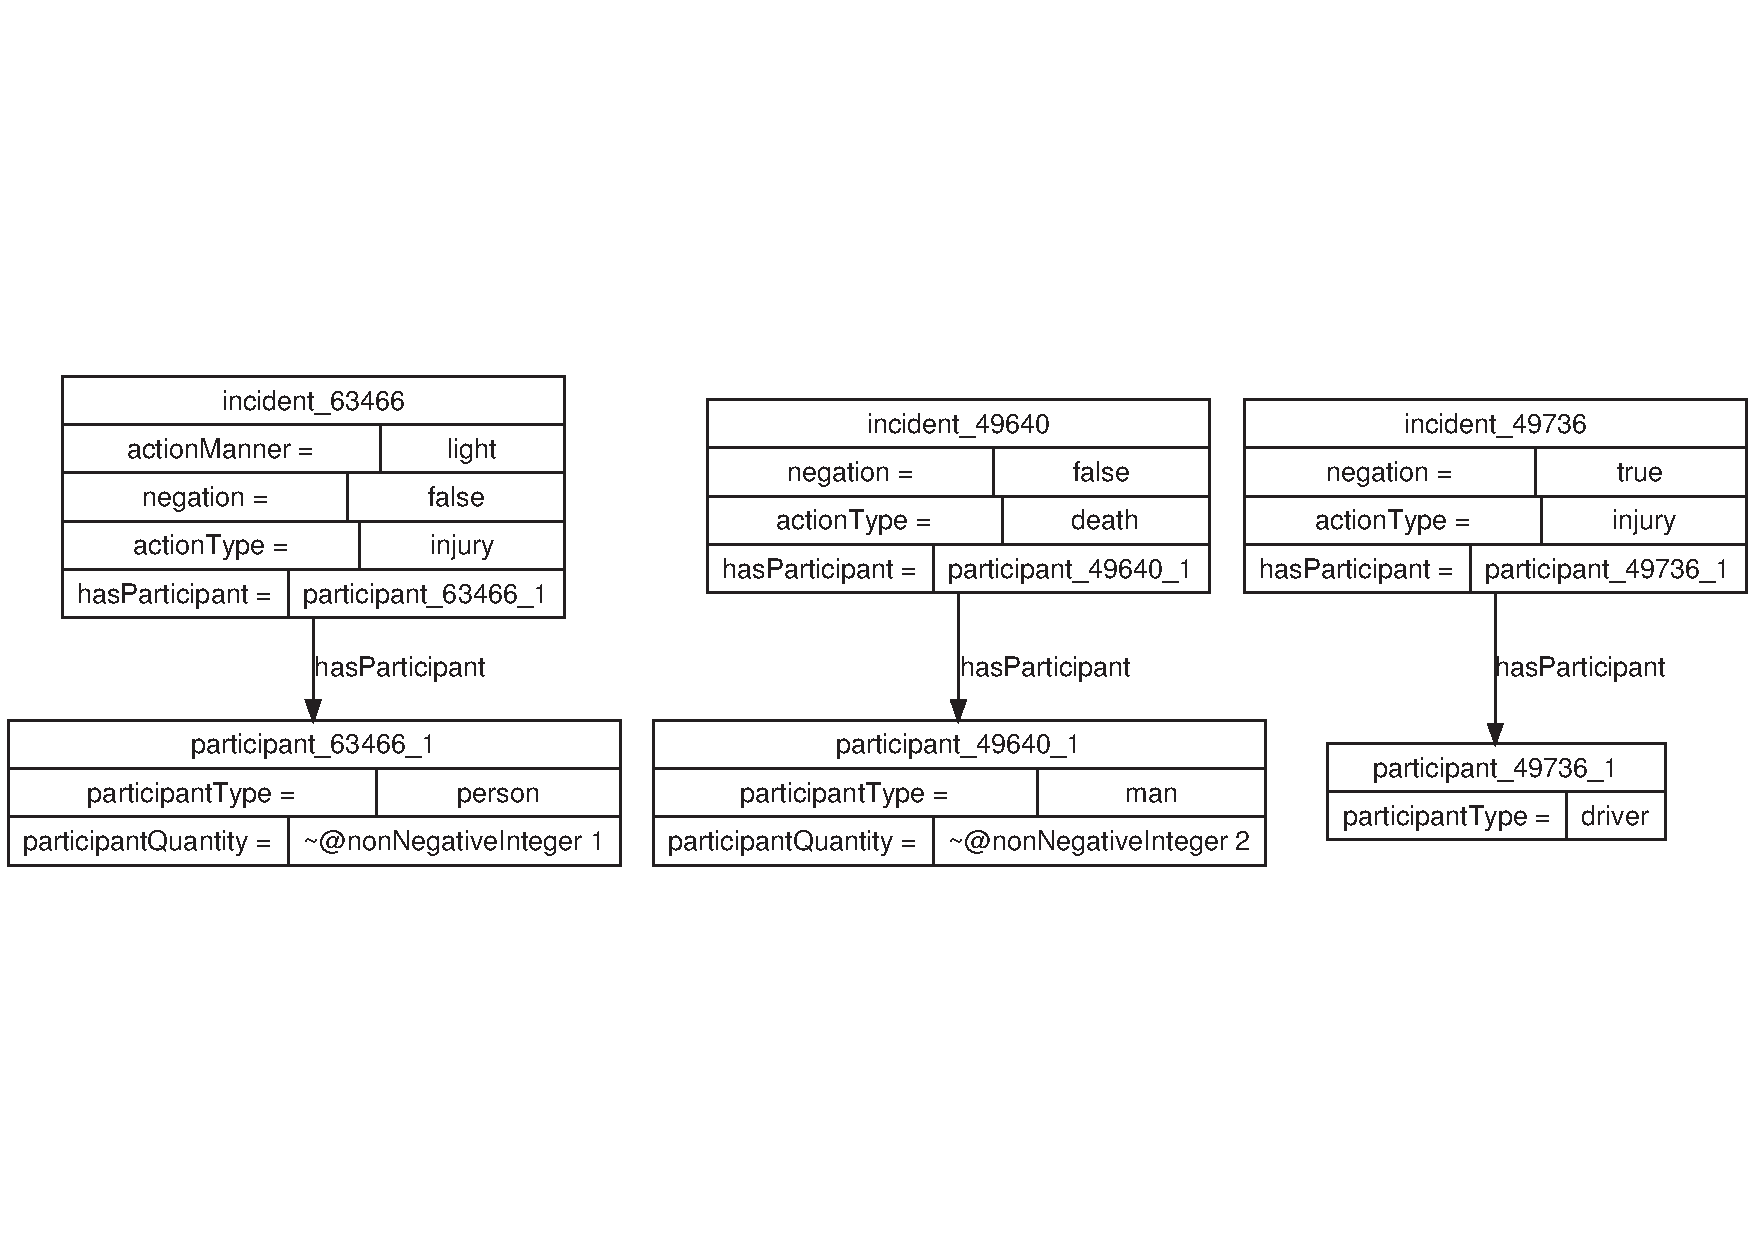
\includegraphics[angle=-90, width=\hsize]{instances}
	\caption{Extracted instances of the target ontology.}
	\label{fig:manual_instatnces}
\end{figure}

\begin{figure}
	\centering
		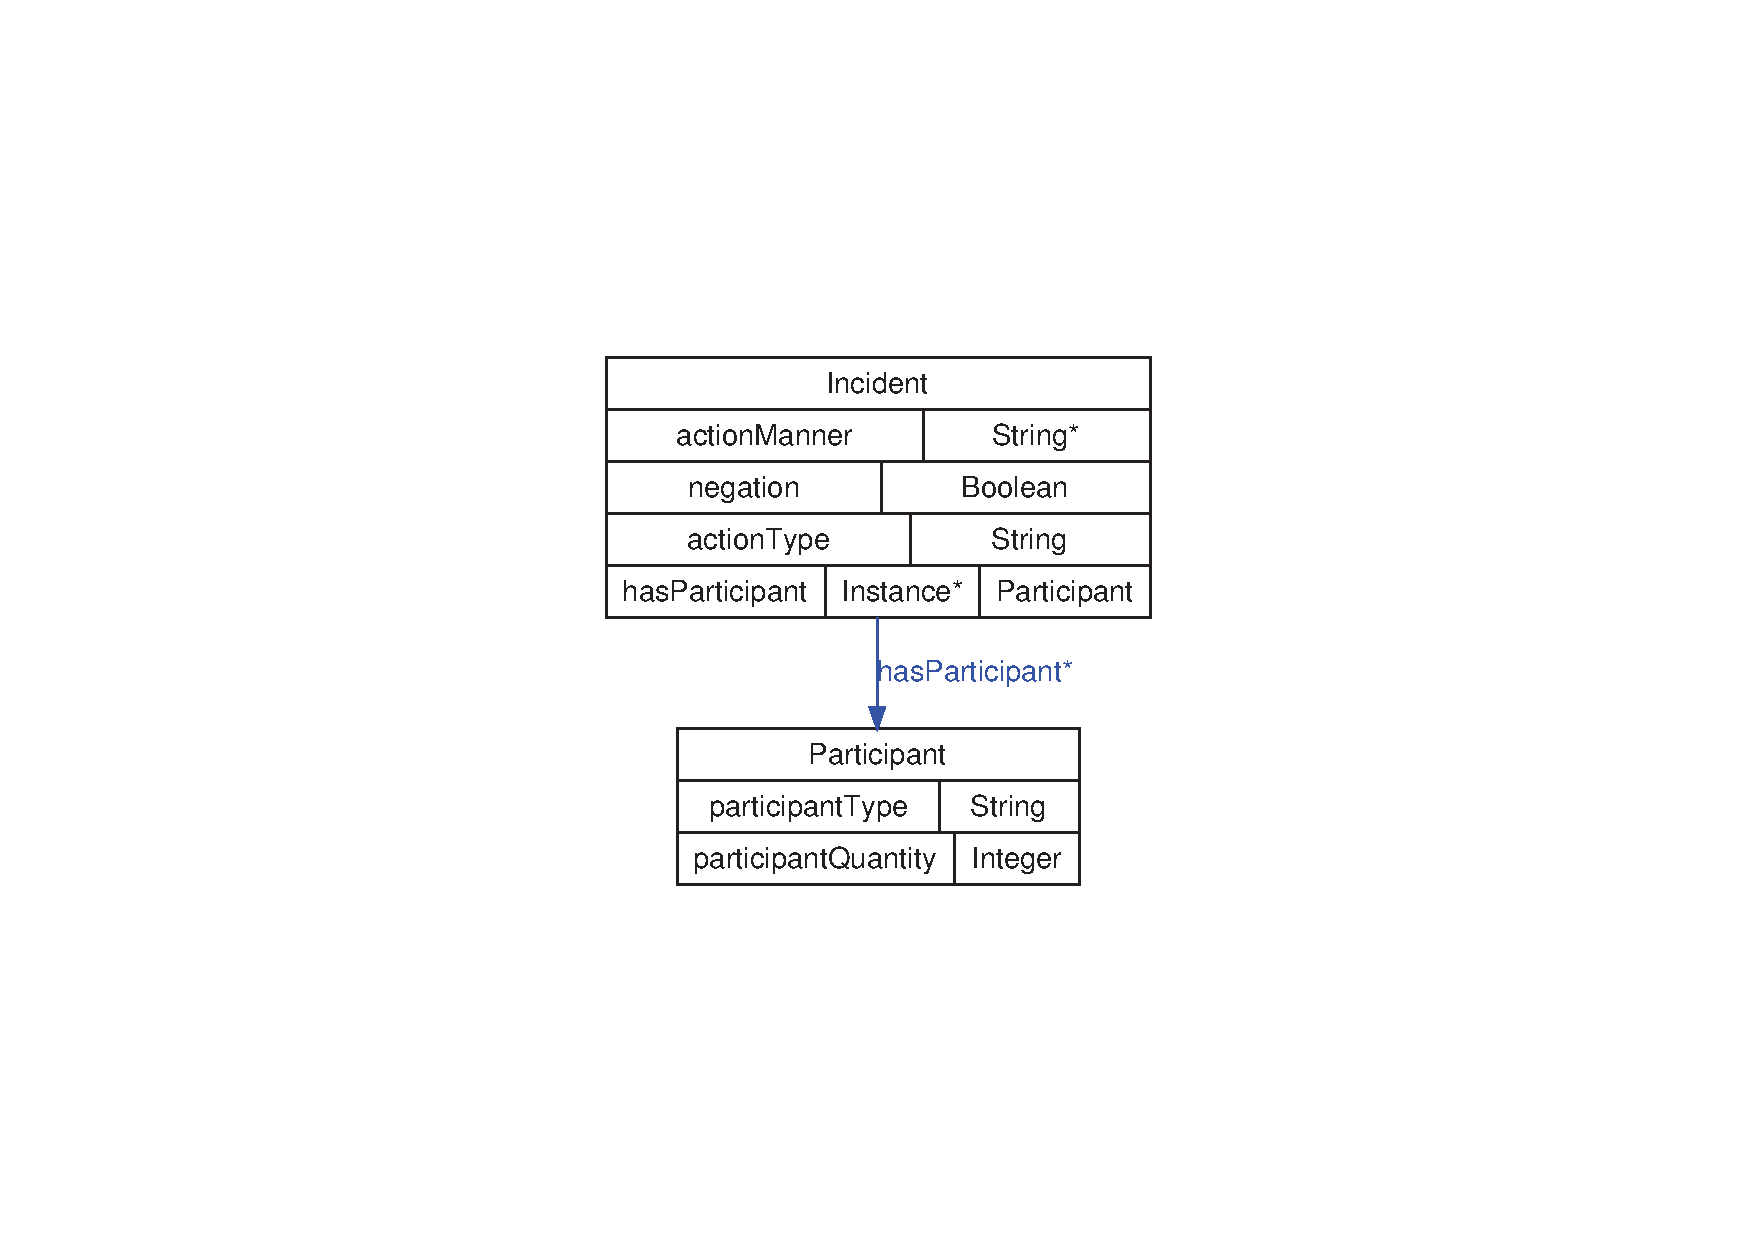
\includegraphics[angle=-90, width=0.3\hsize]{classes}
	\caption{Schema of the target ontology.}
	\label{fig:manual_classes}
\end{figure}

%%%%%%%%%%%%%%%%%%%%%%%%%%%%%%%%%%%%%%%%%%%%%%%%%%%%%%%%%%%%%%%%%%%%%%%%%%%%%%%%%%%%%
\begin{figure}
\begin{minted}[linenos,  fontsize=\footnotesize,
               frame=lines]{sparql}

SELECT ?action ?participant ?participant_type ?quantity
WHERE {
	{
		?action rdf:type :Incident;
			:actionType "death";
			:negation false.
	} UNION {
		?action rdf:type :Incident;
			:actionType "survival";
			:negation true.
	}
	?action :hasParticipant ?participant.
	?participant :participantType ?participant_type.
	OPTIONAL {
		?participant :participantQuantity ?quantity.
	}
}
\end{minted}
\caption{\emph{SPARQL} query that summarizes fatalities of particular incidents.}
\label{fig:sparql_aggregation}
\end{figure}
%%%%%%%%%%%%%%%%%%%%%%%%%%%%%%%%%%%%%%%%%%%%%%%%%%%%%%%%%%%%%%%%%%%%%%%%%%%%%%%%%%%%%



Similar but in a sense different solution is to ground the mapping directly in extraction rules. Instead of creating mapping of the extraction output, extraction rules will contain also the information about the form of the extraction output. Selection of particular query nodes and linguistic attributes for the output will be extended by the specification of how the attributes will be rendered on the output. A graphical representation of such extraction rule can look like in Figure~\ref{fig:manual_semantic_interpretation}. It shows the connection between a Netgraph query on the left and an ontology instance on the right. Every node of the query can be translated to the ontology and the translation can be configured. 

The configurable translations are the most interesting part of these extraction rules. The linguistic information on one side has to be converted to the ontological information on the other side. In Figure~\ref{fig:manual_semantic_interpretation}, following translation types were used: a translation of numerals to numbers, lexical translation from a source language (Czech), and detection of negation present in a query node.

For better illustration, Figure~\ref{fig:manual_instatnces} shows how the extraction output would look like in the semantic case\footnote{The same data will be used in the next chapter in the example of raw extraction output (Figure~\ref{fig:select_xml}).}. The presented ontology was designed only for the illustration. Schema of the ontology can be seen in the Figure~\ref{fig:manual_classes}. It consists of two classes (or concepts): \emph{Incident} and \emph{Participant}. These classes are connected with a relation \emph{hasParticipant}. There are also some data-type properties (\emph{actionType}, \emph{actionManner}, \emph{negation}, \emph{participantType}, \emph{participantQuantity}) to cover the extracted data. 

The last illustration is a SPARQL query (Figure~\ref{fig:sparql_aggregation}) that would display a table of fatalities present in extracted RDF data. The query is based on the previous ontology and it demonstrates possible use of the schema and the extracted data.







%%%%%%%%%%%%%%%%%%%%%%%%%%%%%%%%%%%%%%%%%%%%%%%%%%%%%%%%%%%%%%%%%%%%%%%%%%%%%%%%%%%%%
%%%%%%%%%%%%%%%%%%%%%%%%%%%%%%%%%%%%%%%%%%%%%%%%%%%%%%%%%%%%%%%%%%%%%%%%%%%%%%%%%%%%%
%%%%%%%%%%%%%%%%%%%%%%%%%%%%%%%%%%%%%%%%%%%%%%%%%%%%%%%%%%%%%%%%%%%%%%%%%%%%%%%%%%%%%
\section{Machine Learning of Extraction Rules} \label{sec:learning_methods} \graphicspath{{../img/ch60/}}

In this section we present %main results and reflections of our ongoing PhD project, 
our method for information extraction and annotation of texts, which is based on a deep linguistic analysis and Inductive Logic Programming (ILP) and implemented with the great help of the GATE framework. This approach is quite novel because it directly combines deep linguistic parsing with machine learning (ML). This combination and the use of ILP as a ML engine have following benefits: Manual selection of learning features is not needed. 
The learning procedure has full available linguistic information at its disposal and it is capable to select relevant parts itself. Extraction rules learned by ILP can be easily visualized, understood and adapted by human.


\subsection{Data Flow}


Similarly to the previous case with manually designed rules, also this extraction method was designed as a method for extraction of information from web resources and the goal is in extracted data in the form of semantic web ontology. The schema of the extraction process is different than the one presented in the previous section because it includes also the learning phase when extraction rules are learned from a learning collection. The present schema can be found on Figure~\ref{fig:ILP_data_flow}, it is an adaptation of the general schema presented in Section~\ref{sec:third_gate_ML}. The schema is a little complicated because it illustrates two cases (or phases) in one picture:
\begin{enumerate}
	\item the learning phase and
	\item the application phase when existing extraction rules are applied to new documents and new information is being extracted.
\end{enumerate}

\subsubsection{Learning Phase}
We will start the description with the learning phase and we will start on the Web (upper left corner of the schema). We need to obtain a learning collection of texts. They can be found on the web (the violet cloud), downloaded and text has to be extracted form them (the texts image). Now we need a human annotator (the worker image bellow), who will look at each of the texts and create gold standard annotations for these texts. These steps can be done using the GATE framework and we will not describe them further. 

Before we can execute the learning procedure of Inductive Logic Programming (green circle), three more steps have to be done:
\begin{enumerate}
	\item perform automated linguistic analysis, which will construct linguistic trees from the texts,
	\item transform these linguistic trees to ILP background knowledge and
	\item transform the gold standard annotations to ILP learning examples.
\end{enumerate}
These steps will be described in following sections and in the next chapter about implementation (Section~\ref{sec:learning_impl}). The ILP learning procedure will produce extraction rules (orange oval) that will be used in the application phase.

\subsubsection{Application Phase}
Again, let us start the description on the web. Assume that target web pages for extraction have been identified, text extracted from them and linguistic trees constructed from the text. In this phase, we do not need ILP, but ordinary Logic Programming is still used for deciding which linguistic trees are covered by extraction rules. Therefore, again, the linguistic trees have to be transformed to ILP background knowledge.
 The previously learned extraction rules are applied on the ILP background knowledge constructed from the new trees during the main extraction process (green circle in the top right corner of the schema) and it will produce new extracted data with the same semantics that was used during manual annotation.

\begin{figure}
	\centering
		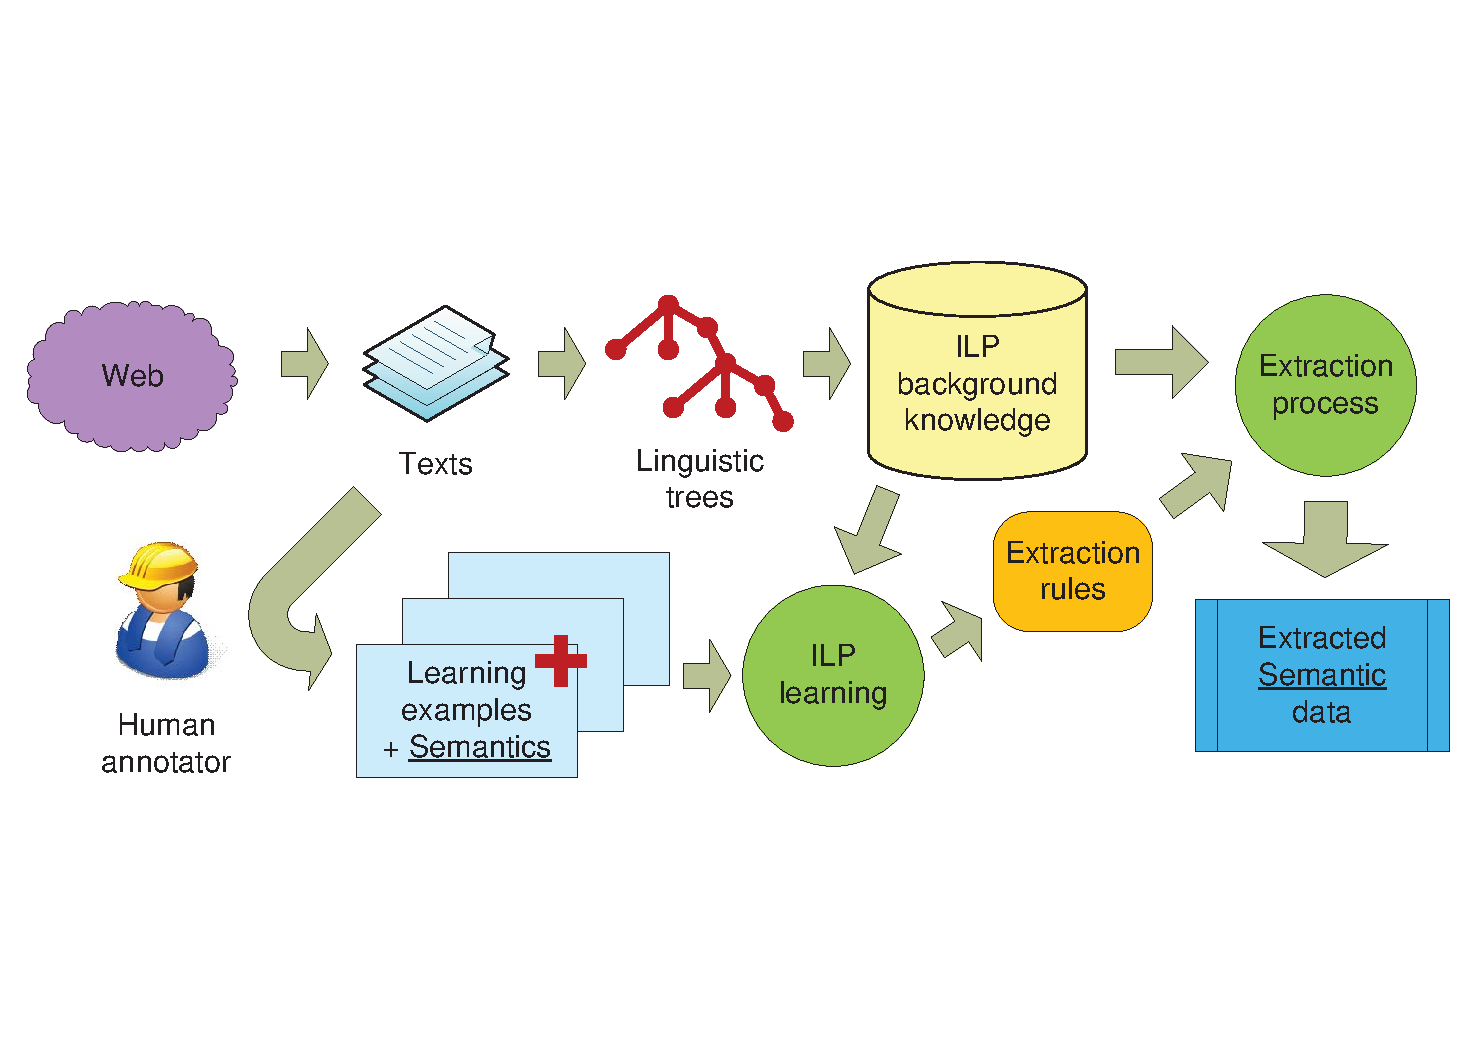
\includegraphics[angle=-90, width=0.85\hsize]{ILP_data_flow}
	\caption{ILP data flow.}
	\label{fig:ILP_data_flow}
\end{figure}


\subsection{Closer Investigation}
The description of the data flow schema in the previous section was quite general, not containing any implementation specific details. In this section, we want to provide more details about the actual realization of that general data flow because some interesting problems are connected with it.

First of all, the interface of this extraction method is different from the previously described method based on manually designed extraction rules. The previous method was realized as purely information extraction method while this method performs document annotation and therefore the correspondence of extracted information with its position in text has to be preserved, see details in following sections. 

Another difference with the previous approach is that the previous approach is based on Netgraph and Netgraph is responsible for the management of linguistic trees in that case. The present method is based on GATE and ILP and these tools do not provide any special functions for working with linguistic trees. These functions were added by us and they provide:
\begin{itemize}	
	\item conversion of PDT linguistic trees to GATE annotations (see details in Section~\ref{sec:learning_pdt_in_gate}) and the possibility of calling TectoMT linguistic analysis directly from GATE (see details in Section~\ref{sec:learning_tectomt_wrapper}) and
	
	\item integration of Prolog and ILP with GATE (see details in Section~\ref{sec:learning_ilp_wrapper}), which includes conversion of GATE annotations and the linguistic tree structure to ILP background knowledge (see details in Section~\ref{sec:learning_ilp_serialization}).
\end{itemize}





\subsection{Correspondence of GATE Annotations with Tree Nodes}

On the one hand, our extraction method is based on linguistic trees that are composed of individual tree nodes, but on the other hand, we are performing document annotation using GATE, which means that annotations can occupy any segment of text, e.g. a segment starting or ending in the middle of some word. The correspondence of tree nodes with individual words (or tokens) of text is quite clear\footnote{Tectogrammatical tree nodes make it a little more difficult, see details in Section~\ref{sec:third_PDT_layers}.} but the learning algorithm is not capable to deal with partial word matches. This is not a problem in the case when annotations discovered by the extraction technique are put to the text because all the annotations will simply occupy whole words only. The problem can occur when ILP learning data are constructed from GATE annotations. During this construction, only those tree nodes that are completely covered by corresponding annotations will be accordingly marked in the ILP learning data.

%kvuli footenote-um, aby se vesly...
\pagebreak

Let us for example have a phrase ``eight thousand Crowns’’ and an annotation labeled as ``amount’’ that will almost cover the whole phrase up to the word ``Crowns’’, which will be covered only partly, without the ending ``s’’. Thus the annotated text will be ``eight thousand Crown’’.\footnote{Such annotation could be created by an uninformed annotator who could think that currencies should be marked as in singular form.} During the construction of ILP learning data, only the tree nodes corresponding to words ``eight’’ and ``thousand’’ will be marked as ``amount’’, not the node that corresponds with the word ``Crowns’’.

Fortunately, this phenomenon does not occur very often, in fact we have not met it in our experiments so far. But there is another issue that is connected with multi-word annotations and it is quite common. See in the next section.


\subsection{Root/Subtree Preprocessing/Postprocessing} \label{sec:learning_root_subtree}
Sometimes annotations span over more than one token. This situation complicates the process of machine learning and this situation is often called as ``chunk learning''. Either we have to split a single annotation to multiple learning instances and after the application of extraction rules we have to merge them back together, or we can change the learning task from learning annotated tokens to learning borders of annotations (start tokens and end tokens). The later approach is implemented in GATE in \emph{Batch Learning PR}\footnote{\url{http://gate.ac.uk/userguide/sec:ml:batch-learning-pr}} in the `SURROUND' mode.

We have used another approach to solve this issue. Our approach is based on syntactic structure of a sentence and we call it ``root/subtree preprocessing/postprocessing''. The idea is based on the observation that tokens of a multi-token annotation usually have a common parent node in a syntactic tree. So we can
\begin{enumerate}
	\item extract the parent nodes (in dependency linguistics this node is also a token and it is usually one of the tokens inside the annotation), 
	\item learn extraction rules for parent nodes only and 
	\item span annotations over the whole subtrees of root tokens found during the application of extraction rules.
\end{enumerate}
We call the first point as \emph{root preprocessing} and the last point as \emph{subtree postprocessing}. The situation is illustrated on Figure~\ref{fig:tree-subtree}. We have successfully used this technique for the `damage' task of our evaluation corpus (see Section~\ref{sec:learning_eval} for details.)

\begin{figure}
	\centering
		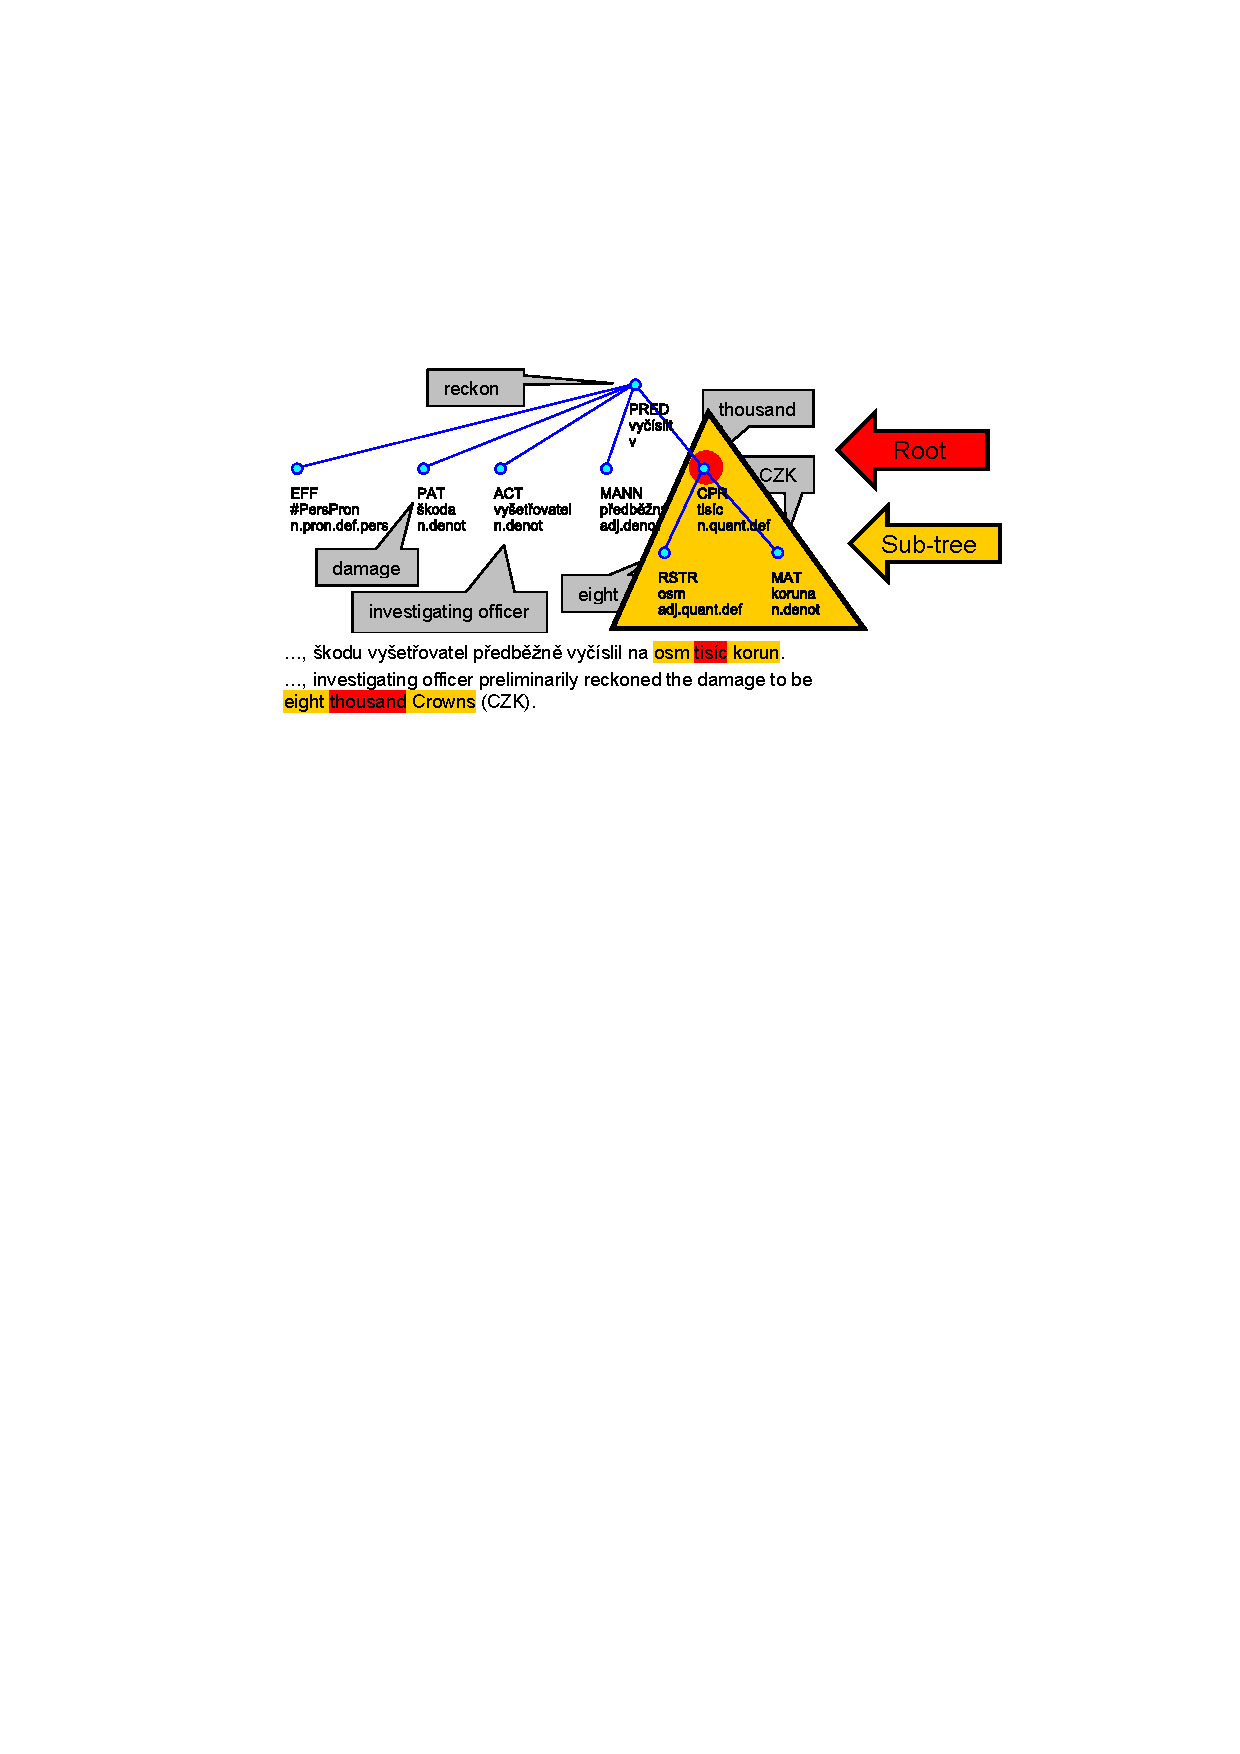
\includegraphics[width=0.85\hsize]{tree-subtree}
	\caption{Root/Subtree Preprocessing/Postprocessing example, see also Figure~\ref{fig:intro_damage_tree} with the original tree.}
	\label{fig:tree-subtree}
\end{figure}


\subsection{Learning on Named Entity Roots} \label{sec:learning_ne_roots}
Another technique, that we have used to improve the efficiency of ILP machine learning, is closely connected with named entities. It can be used when target entities of an extraction task always (or most often) overlap with annotations of some available type (e.g. named entity). For example entities of the task `acquired' always overlap with some named entity, or in other words, `acquired' entities are merely a special case of named entities.

In this case, the extraction task can be rephrased as ``decide which of the named entities belong to the extraction task.'' The collection of learning examples is reduced only to named entities and the learning algorithm is then faster and can be also more accurate.

In order to ILP had the opportunity to decide about these named entities, they have to be connected with additional information present in linguistic trees. But how to connect a potentially multi-token named entity with the nodes of linguistic trees? One possibility is to connect each named entity with all tree nodes it occupies but we have used a simpler solution when only the root token of a named entity is connected.

This solution was used for the majority of extraction tasks of the Acquisitions dataset; see evaluation details in Section~\ref{sec:learning_eval_acq}.

\subsection{Semantic Interpretation} \label{sec:SemanticInterpretation}

Information extraction can solve the task ``how to get documents annotated'', but as we aim on the semantic annotation, there is a second step of ``semantic interpretation'' that has to be done. In this step we have to interpret the annotations in terms of a standard ontology. On a very coarse level this can be done easily. Thanks to GATE ontology tools \citep{Bon04b} we can convert all the annotations to ontology instances with a quite simple JAPE \citep{Cunningham00jape:a} rule, which takes the content of an annotation and saves it as a label of a new ontology instance or as a value of some property of a shared ontology instance. For example in our case of traffic and fire accidents, there will be a new instance of an accident class for each document and the annotations would be attached to this instance as values of its properties. Thus from all annotations of the same type, instances of the same ontology class or values of the same property would be constructed. This is very inaccurate form of semantic interpretation but still it can be useful. It is similar to the GoodRelation \citep{DBLP:conf/ekaw/Hepp08} design principle of \emph{incremental enrichment}\footnote{\url{http://www.ebusiness-unibw.org/wiki/Modeling_Product_Models#Recipe:_.22Incremental_Enrichment.22}}:

\begin{quote}
``...you can still publish the data, even if not yet perfect. The Web will do the rest -- new tools and people.''	
\end{quote}

But of course we are not satisfied with this fashion of semantic interpretation and we plan to further develop the semantic interpretation step as a sophisticated ``annotation $\rightarrow$ ontology'' transformation process that we have proposed in one of our previous works \citep{biblio:DeVoComputingaggregations2008}.



%kvuli footenote-um, aby se vesly...
\clearpage


%%%%%%%%%%%%%%%%%%%%%%%%%%%%%%%%%%%%%%%%%%%%%%%%%%%%%%%%%%%%%%%%%%%%%%%%%%%%%%%%%%%%%
%%%%%%%%%%%%%%%%%%%%%%%%%%%%%%%%%%%%%%%%%%%%%%%%%%%%%%%%%%%%%%%%%%%%%%%%%%%%%%%%%%%%%
%%%%%%%%%%%%%%%%%%%%%%%%%%%%%%%%%%%%%%%%%%%%%%%%%%%%%%%%%%%%%%%%%%%%%%%%%%%%%%%%%%%%%

\section{Shareable Extraction Ontologies} \label{sec:onto_extraction_ontologies}
\graphicspath{{../img/ch70/}}

In this section we present an extension of the idea of extraction ontologies that was originally presented by \cite{DBLP:conf/er/EmbleyTL02}. We adopt the point that extraction models are kept in extraction ontologies and we add that the extraction ontologies should not be dependent on the particular extraction/annotation tool. In such case the extraction/annotation process can be done separately by an ordinary reasoner.


We present a proof of concept for the idea: a case study with our linguistically based IE engine and an experiment with several OWL reasoners. In the case study (see Section~\ref{sec:onto_case}) the IE engine exports its extraction rules to the form of an extraction ontology. Third party linguistic tool linguistically annotates an input document and the linguistic annotations are translated to so-called document ontology. After that an ordinary OWL reasoner is used to apply the extraction ontology on the document ontology, which has the same effect as a direct application of the extraction rules on the document. The process is depicted in Figure~\ref{fig:rules_app_schema} and it will be described in detail in Section~\ref{sec:onto_case}.



The most closely related work was already presented in Section~\ref{sec:relwork_ext_ont}. The main idea will be illustrated on our case study in Section~\ref{sec:onto_case}, its implementation in Section~\ref{sec:onto_implement} and in Section~\ref{sec:onto_experiment} an experiment with several OWL reasoners and IE datasets will be presented. In Section~\ref{sec:onto_discuss} related issues are discussed and Section~\ref{sec:onto_conclusion} concludes the discussion.

\subsection{Document Ontologies and Annotated Document Ontologies} \label{sec:onto_doc_ont}

The idea of shareable extraction ontologies assumes that extraction ontologies will be shareable and they can be applied on a document outside of the original extraction/annotation tool. We further assert that the extraction ontologies can be applied by ordinary reasoners. This assumption implies that both extraction ontologies and documents have to be in a reasoner readable format. In the case of contemporary OWL reasoners there are standard reasoner-readable languages: OWL and RDF in a rich variety of possible serializations (XML, Turtle, N-Triples, etc.) Besides that there exists standard ways like GRDDL or RDFa how to obtain a RDF document from an ``ordinary document'' (strictly speaking XHTML and XML documents).

We call `document ontology' an ontology that formally captures content of a document. A document ontology can be for example obtained from the source document by a suitable GRDDL transformation (as in our experiment). A document ontology should contain all relevant data of a document and preferably the document could be reconstructed from the document ontology on demand.

When a reasoner is applying an extraction ontology to a document, it only has ``to annotate'' the corresponding document ontology, not the document itself. Here ``to annotate'' means to add new knowledge -- new class membership or property assertions. In fact it means just to do the inference tasks prescribed by the extraction ontology on the document ontology. 

Obviously when a document can be reconstructed from its document ontology (this is very often true, it is necessary just to save all words and formatting instructions) then also an annotated document can be reconstructed from its annotated document ontology. 





%%%%%%%%%%%%%%%%%%%%%%%%%%%%%%%%%%%%%%%%%%%%%%%%%%%%%%%%%%%%%%%%%%%%%%%%%%%%%%%%%%%%%%%%%%%%%%%%%%%%%%%%%%%%%%
\subsection{The Main Idea Illustrated -- a Case Study} \label{sec:onto_case}
%%%%%%%%%%%%%%%%%%%%%%%%%%%%%%%%%%%%%%%%%%%%%%%%%%%%%%%%%%%%%%%%%%%%%%%%%%%%%%%%%%%%%%%%%%%%%%%%%%%%%%%%%%%%%%

In this section, realization of the main idea will be described and illustrated on a case study.

A schema of the case study is presented in Figure~\ref{fig:rules_app_schema}.  
The top row of the image illustrates how TectoMT (third party linguistic tool) linguistically annotates an input document and the linguistic annotations are translated to so-called document ontology by a GRDDL/XSLT transformation.

In the bottom of the picture our IE engine learns extraction rules and exports them to an extraction ontology. The reasoner in the middle is used to apply the extraction ontology on the document ontology and it produces the ``annotated'' document ontology, which was described in the previous section.


\begin{figure}
\centerline{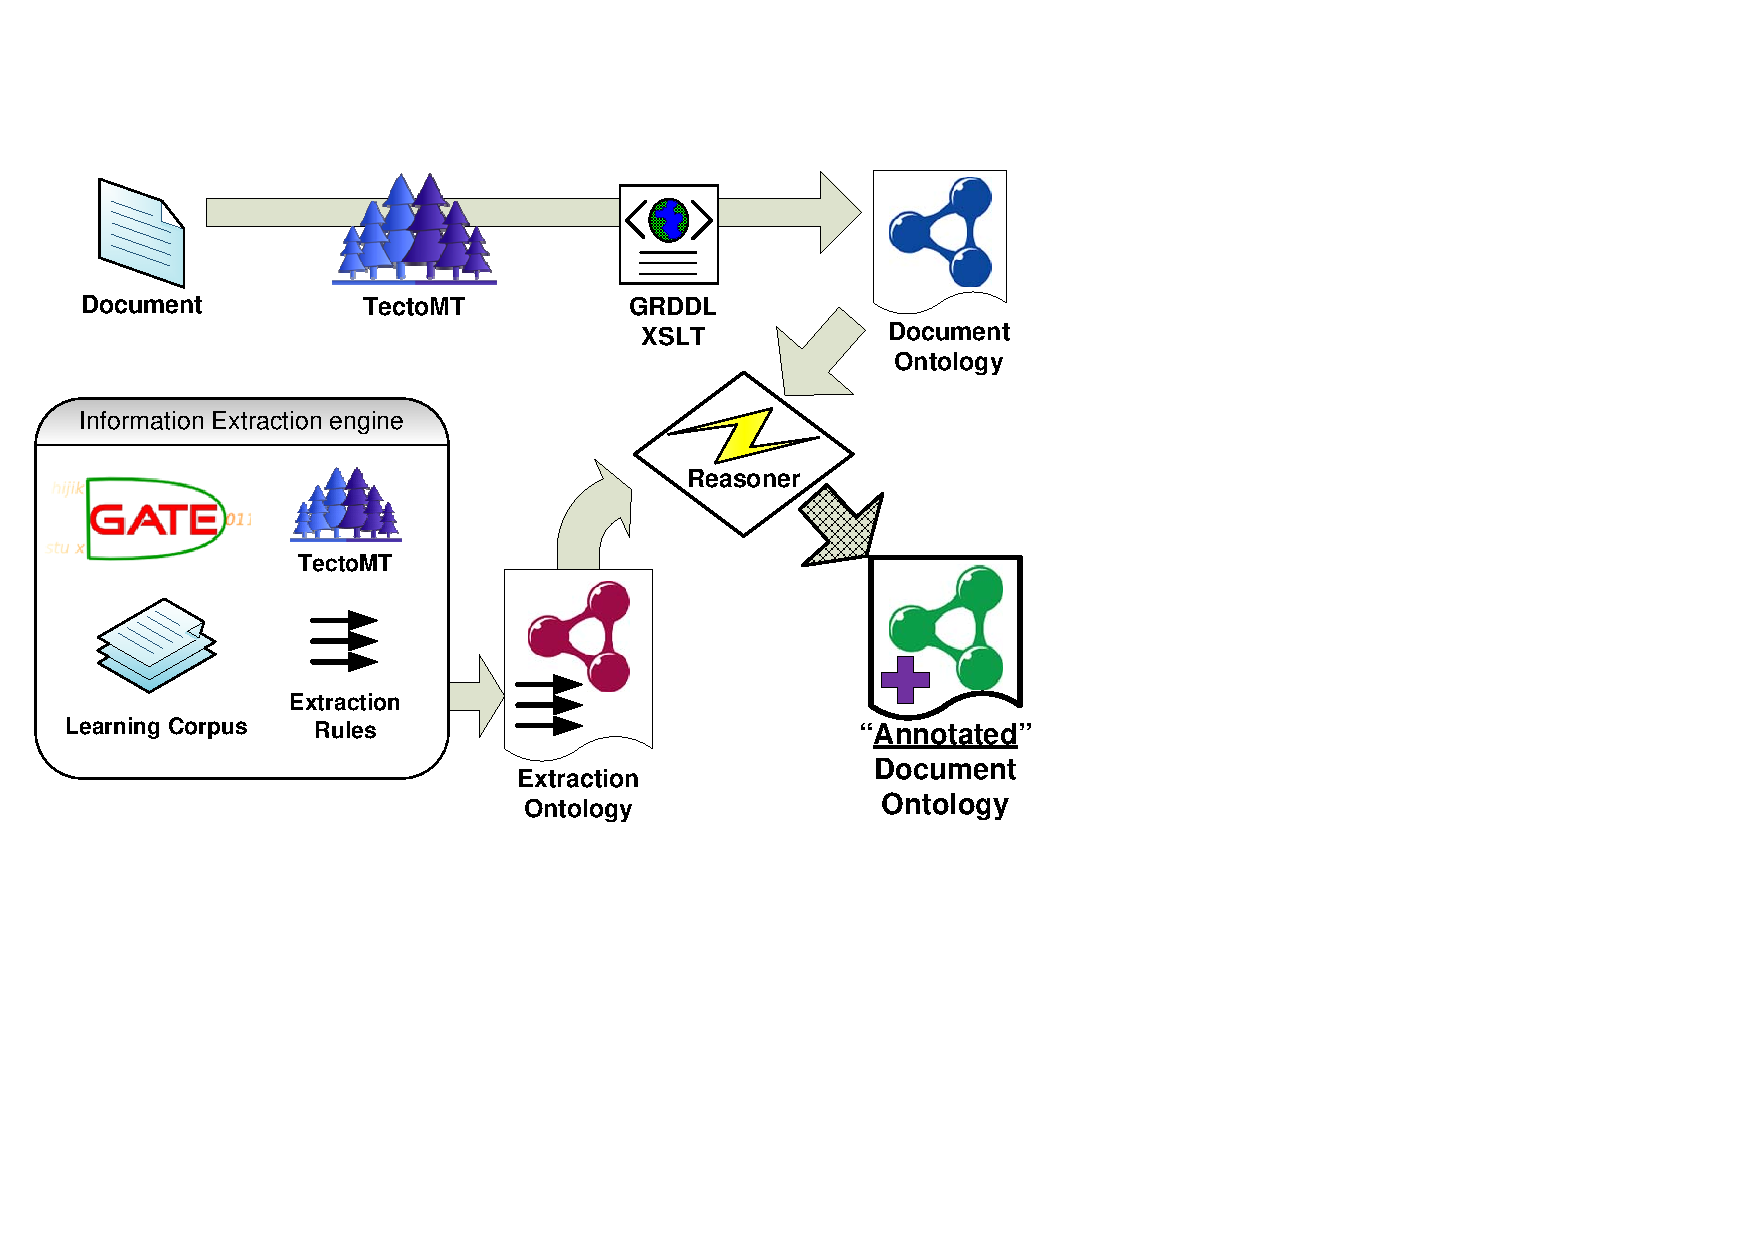
\includegraphics[angle=-90, width=0.7\hsize]{semantic_rules_app_schema}}
\caption{Semantic annotation driven by an extraction ontology and a reasoner -- schema of the process.}
\label{fig:rules_app_schema}
\end{figure}

Implementation of the case study will be described in Section~\ref{sec:onto_implement}. It exploits the approaching support for Semantic Web Rule Language (SWRL) \citep{SWRL}. Although SWRL is not yet approved by W3C it is already widely supported by Semantic Web tools including many OWL reasoners. The SWRL support makes it much easier to transfer the semantics of extraction rules used by our IE tool to extraction ontology. The translation of the native extraction rules to SWRL rules that form the core of the extraction ontology will be also presented in Section~\ref{sec:onto_implement}.







%%%%%%%%%%%%%%%%%%%%%%%%%%%%%%%%%%%%%%%%%%%%%%%%%%%%%%%%%%%%%%%%%%%%%%%%%%%%%%%%%%%%%%%%%%%%%%%%%%%%%%%%%%%%%%
%%%%%%%%%%%%%%%%%%%%%%%%%%%%%%%%%%%%%%%%%%%%%%%%%%%%%%%%%%%%%%%%%%%%%%%%%%%%%%%%%%%%%%%%%%%%%%%%%%%%%%%%%%%%%%
%%%%%%%%%%%%%%%%%%%%%%%%%%%%%%%%%%%%%%%%%%%%%%%%%%%%%%%%%%%%%%%%%%%%%%%%%%%%%%%%%%%%%%%%%%%%%%%%%%%%%%%%%%%%%%
\section{Fuzzy ILP Classification} \label{sec:fuzzy_methods}
\graphicspath{{../img/ch80/}}

In this section, we study the problem of classification of textual reports. We are %specifically
 focused on the situation in which structured information extracted from the reports is used for such classification. We present a~proposal and a partial implementation of an experimental classification system based on our previous work on information extraction (see Sections~\ref{sec:manual_methods} and \ref{sec:learning_methods} for details) and fuzzy inductive logic programming (fuzzy ILP).
Our description is based on a case study of seriousness classification of accident reports. 
%Figure~\ref{fig:message} presents an example of an accident report from a message on the web.
We would like to have a tool that is able to classify the accident's degree of seriousness on the basis of information obtained through information extraction.
%Our approach is based on information extraction and on a fuzzy-based machine learning procedure that provides rules for classification of the reports.
In this section,
% we do not provide any details about the information extraction part of the solution (it was already described in Chapters~\ref{sec:manual_manual_rules_chapter} and \ref{ch:ILP_Learning}). 
we concentrate on the classification part and present a detailed study of the fuzzy ILP classification method (so-called `Fuzzy ILP Classifier'). 

This problem represents a challenge of induction and/or mining on several occasions. First we need an inductive procedure when extracting attributes of an accident from text. Second (the subject of this section) we need an inductive procedure when trying to explain an accident's degree of seriousness by its attributes. ILP is used as the inductive procedure in both of these places.
\begin{itemize}
	\item During the information extraction phase, we exploit the fact that ILP can work directly with multirelational data, e.g., deep syntactic (tectogrammatical) trees built from sentences of the processed text.
	\item During the classification phase, we are experimentally using the Fuzzy ILP Classifier because it performs quite well on our dataset (see Section~\ref{sec:fuzzy_eval}) and it is naturally capable of handling fuzzy data, which occurs when the information extraction engine returns confidence probability values along with extracted data. But the description does not go so far and only the approach is fuzzy in the present demonstration.
\end{itemize}





The rest of this section is organized as follows: Design of the experimental system is presented in Section~\ref{sec:fuzzy_system}. %including a short description of the information extraction method and linguistic analyzers. 
Section~\ref{sec:fuzzy_case} provides details about our case study, which is later used in examples. Formal models of the system (including several translations of a fuzzy ILP task to classical ILP) are presented in Section~\ref{sec:fuzzy_ilp_task_translation}, followed by a description of implementation of the models in the system. In Section~\ref{sec:fuzzy_results} we present the main results of the work, and then we evaluate and compare the methods with other well-known classifiers. Section~\ref{sec:conclusion} concludes the chapter.

See also Section~\ref{sec:relwork_doc_classification}, where some closely related works were introduced. 

 



%%%%%%%%%%%%%%%%%%%%%%%%%%%%%%%%%%%%%%%%%%%%%%%%%%%%%%%%%%%%%%%%%%%%%%%%%%%%%%%%%%%%%%%%%%%%%%%%%
\subsection{Data Flow} \label{sec:fuzzy_system}
%%%%%%%%%%%%%%%%%%%%%%%%%%%%%%%%%%%%%%%%%%%%%%%%%%%%%%%%%%%%%%%%%%%%%%%%%%%%%%%%%%%%%%%%%%%%%%%%%
%\begin{figure}
%\centerline{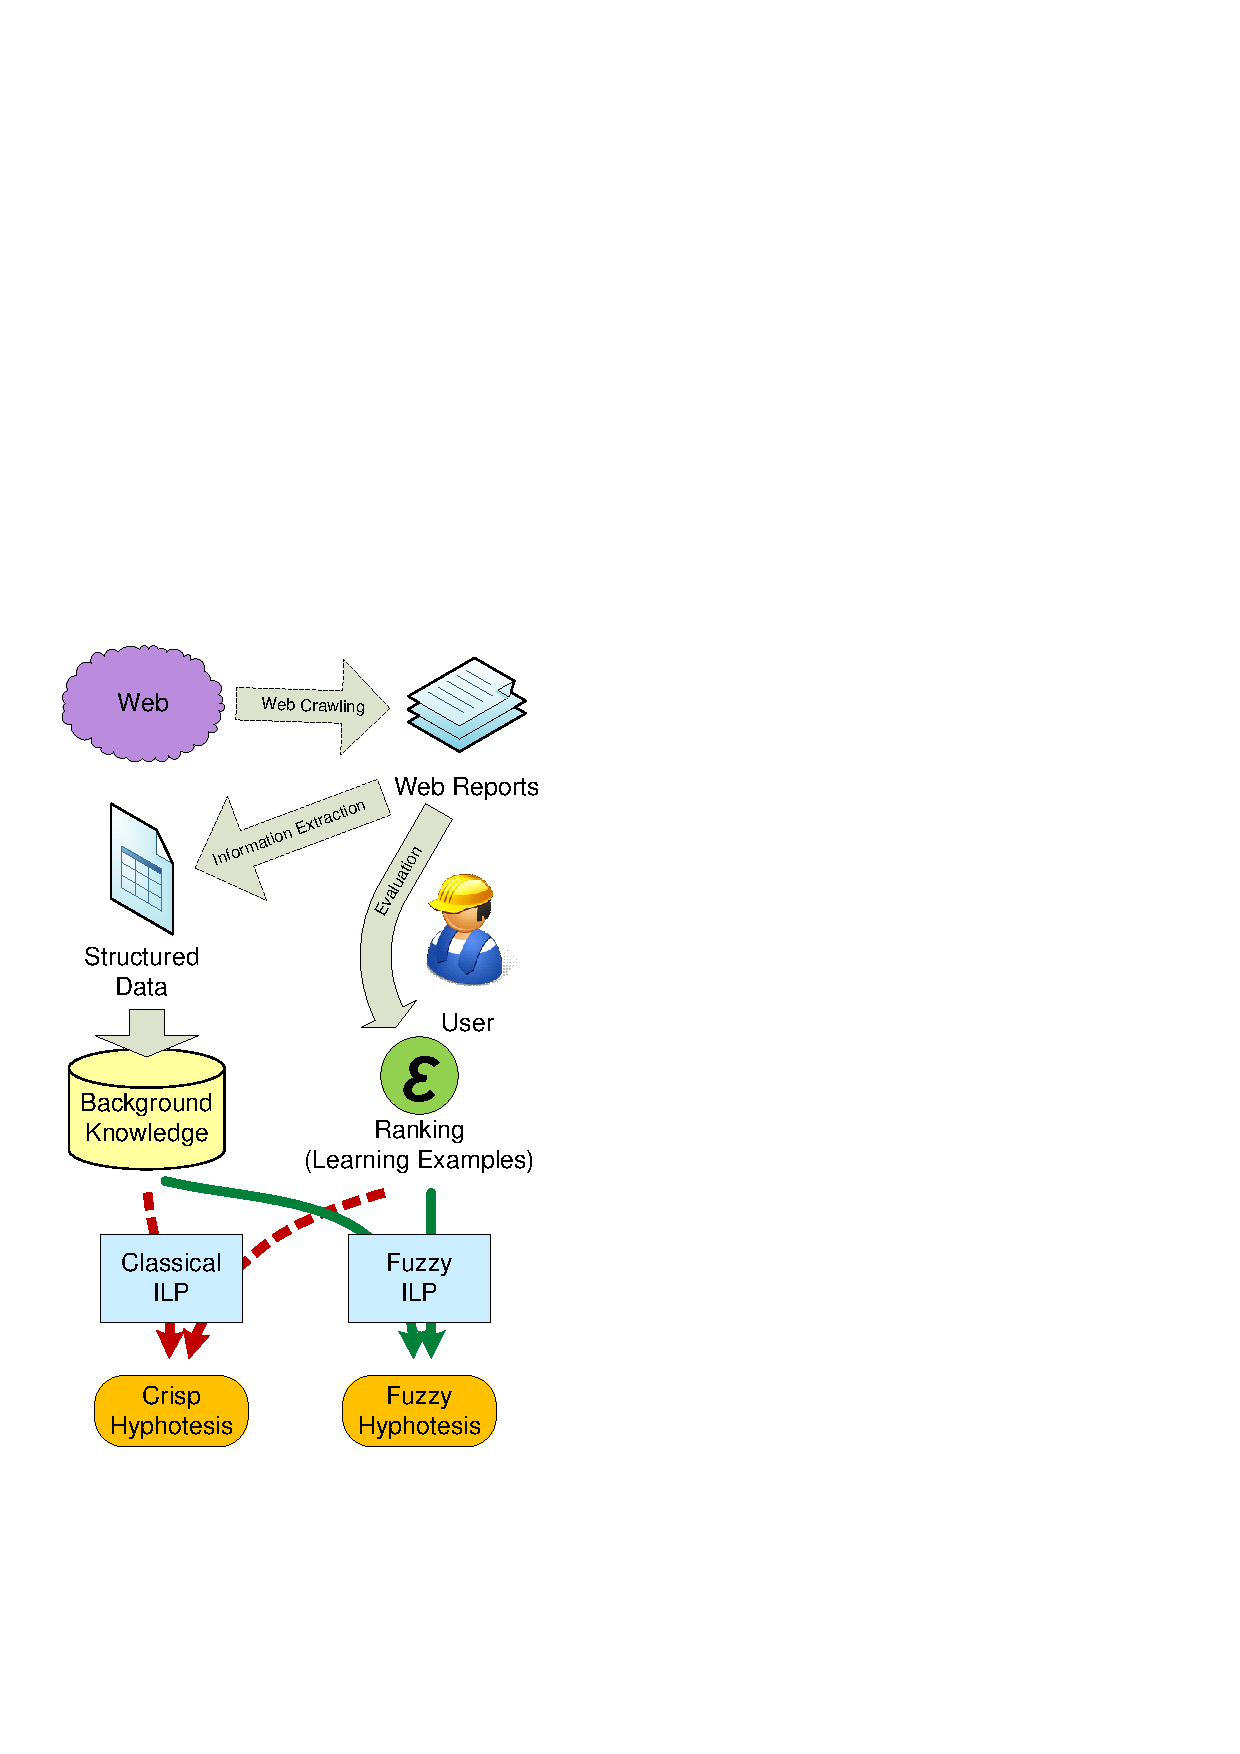
\includegraphics[width=0.4\hsize]{schema}}
%\caption{Schema of the experimental system.}
%\label{fig:schema}
%\end{figure}


\begin{wrapfigure}[27]{r}{.45\hsize}
\vspace{-1.5cm}
\centerline{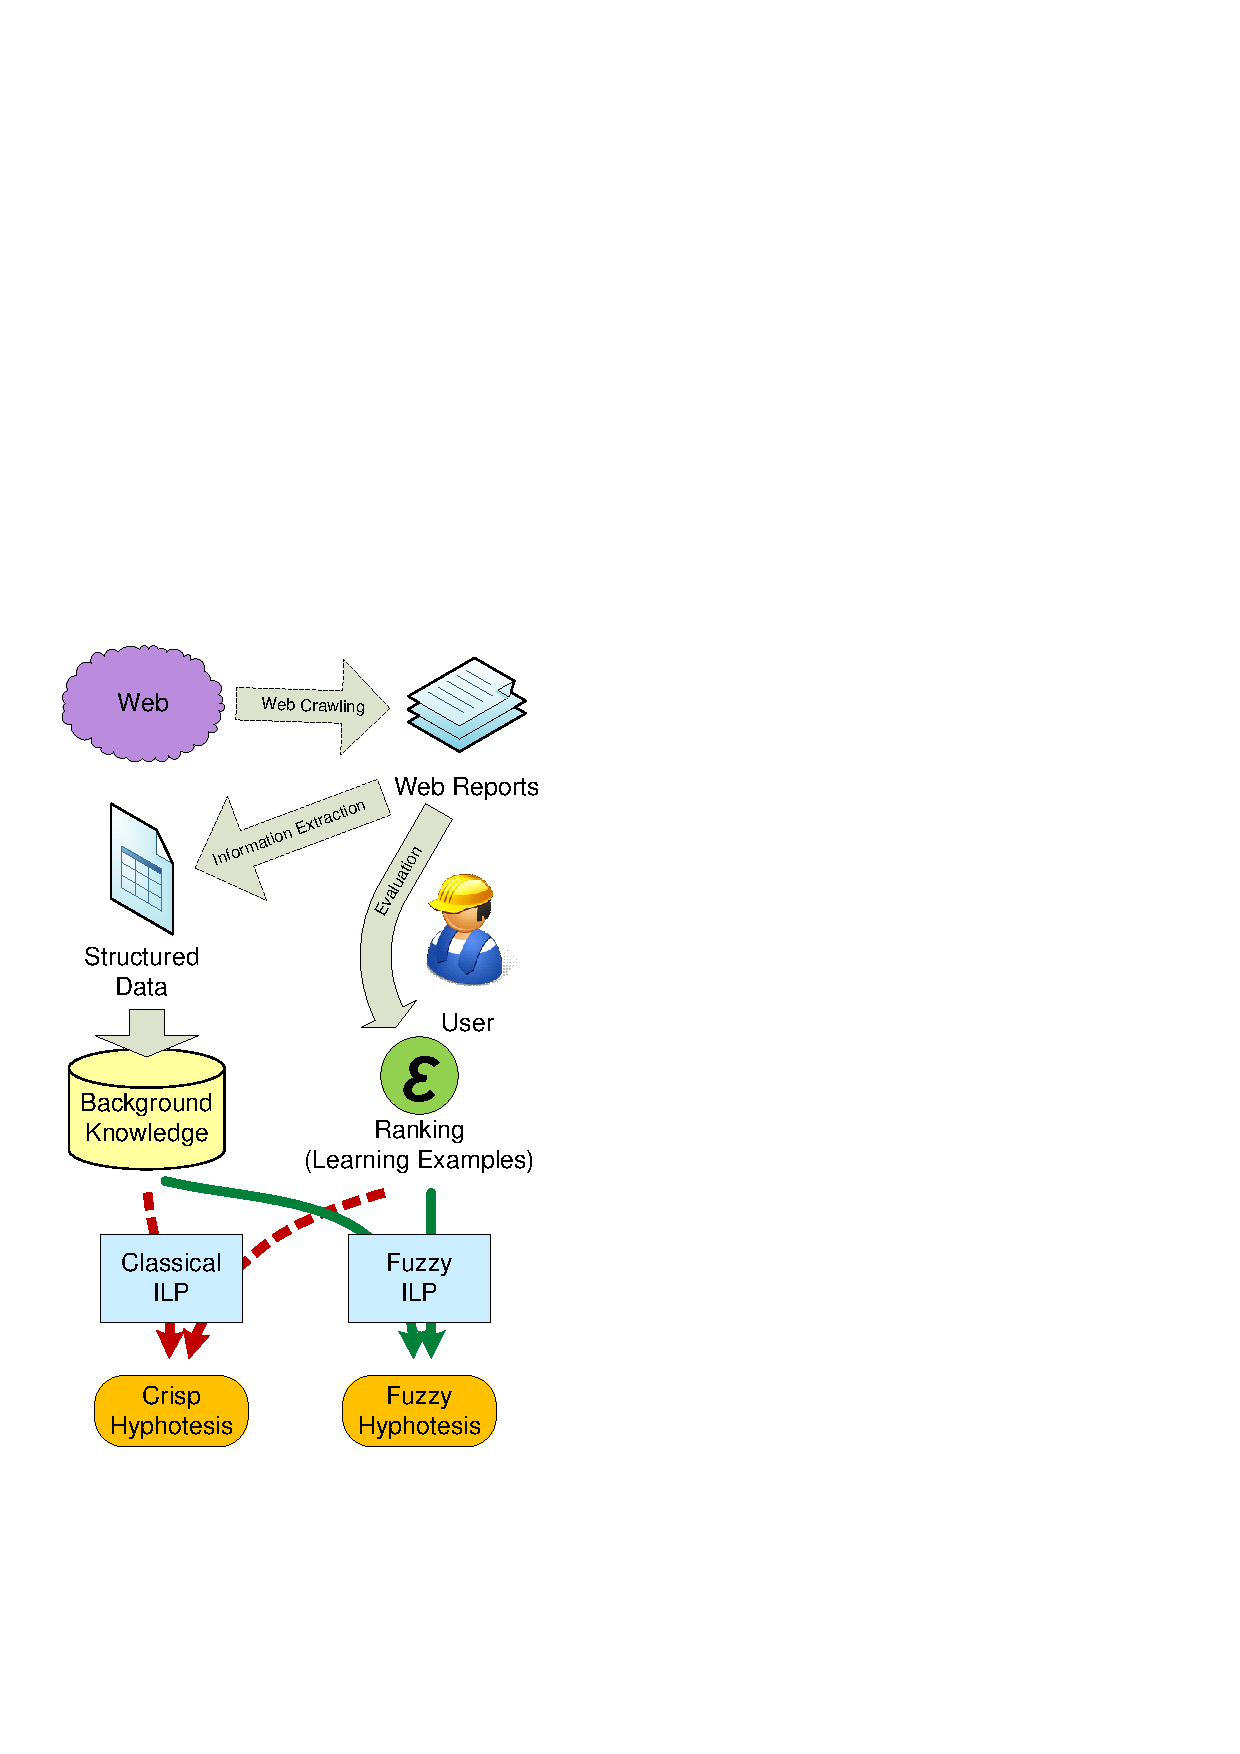
\includegraphics[width=\hsize]{schema}}
\caption{Schema of the experimental system.}
\label{fig:schema}
\end{wrapfigure}


A general schema of the experimental system is shown in Figure~\ref{fig:schema}. In the schema, previously developed information extraction tools based on third party linguistic analyzers are used (the upper two dashed arrows). The information extraction tools are supposed to extract structured information from the reports and the extracted information is then translated to ILP background knowledge and, along with a user rating, it is used for the classification (we assume that a small amount of learning data is annotated by a human user). The classification is based on ILP and it could be \emph{fuzzy} or \emph{crisp}. Crisp denotes a straightforward application of ILP and fuzzy stands for the fuzzy method (subject of the present description), see in the next sections.

\clearpage

%%%%%%%%%%%%%%%%%%%%%%%%%%%%%%%%%%%%%%%%%%%%%%%%%%%%%%%%%%%%%%%%%%%%%%%%%%%%%%%%%%%%%%%%%%%%%%%%%
\subsection{The Case Study -- Accident Seriousness Classification} \label{sec:fuzzy_case}
%%%%%%%%%%%%%%%%%%%%%%%%%%%%%%%%%%%%%%%%%%%%%%%%%%%%%%%%%%%%%%%%%%%%%%%%%%%%%%%%%%%%%%%%%%%%%%%%%



The main experiment leads to the seriousness classification of an accident presented in a report. %Our long term goal is extraction of semantic information from reports. 
%which is one of possible utilizations of the extracted information. 

For the experiment a classification dataset (Section~\ref{sec:data_classify_fireman}) was built based on a collection of 50 textual reports. We have identified several features presented in these reports and manually extracted the corresponding values. To each report we have also assigned a value of overall ranking of seriousness of the presented accident, which is the target of the classification. The dataset is described in Section~\ref{sec:data_classify_fireman}. 
%The whole dataset can be downloaded from our Fuzzy ILP classifier's web page\footnote{\url{http://www.ksi.mff.cuni.cz/~dedek/fuzzyILP/}}.

In the experiment, we have not used any information extracted by our automated information extraction tools. Instead, we concentrate on~the classification; the actual source of the information is not so important for us and the integration step still lies ahead.






%%%%%%%%%%%%%%%%%%%%%%%%%%%%%%%%%%%%%%%%%%%%%%%%%%%%%%%%%%%%%%%%%%%%%%%%%%%%%%%%%%%%%%%%%%%%%%%%%
\subsection{Translation of Fuzzy ILP Task to Several Classical ILP Tasks} \label{sec:fuzzy_ilp_task_translation}
%%%%%%%%%%%%%%%%%%%%%%%%%%%%%%%%%%%%%%%%%%%%%%%%%%%%%%%%%%%%%%%%%%%%%%%%%%%%%%%%%%%%%%%%%%%%%%%%%

Formal definitions of classical and fuzzy ILP tasks were presented in Section~\ref{sec:third_ILP}. In this section, additional formal constructions will be presented, because they are the basis for the implementation.


As far as there is no implementation of fuzzy ILP, we have to use a~classical ILP system. Fortunately, any fuzzy ILP task can be translated to several classical ILP tasks (subject to some rounding and using a finite set of truth values).

Moreover, GAP -- Generalized Annotated Programs \citep{Kifer:1992:TGA:139720.139723} are used in practice, so graded formulas will sometimes be understood as annotated (with classical connectives and with a more complex annotation of the heads of rules). This is possible because \cite{biblio:KLV} showed that (some extension of) fuzzy logic programming is equivalent to (some restriction of) generalized annotated programs. 

The proposed experimental classification system is based on two ILP classification methods -- crisp and fuzzy. 
Technically, the difference between the approaches consists in a different setting of the underlying classical ILP tasks. 
In the following text, translation of the original fuzzy ILP task to the two classical ILP tasks will be presented; the first will be denoted as \emph{crisp}, the second as \emph{monot} (because so called monotonization technique is used). The original \textbf{fuzzy} ILP task can be informally expressed as: ``From a degree of injury, a degree of damage, a degree of duration, etc. determine the degree of seriousness.''   

\bigskip
In the following text, assume that all fuzzy sets take truth values only from a finite set of truth values $T: \{0,1\}\subseteq T\subseteq [0,1]$.

\begin{definition}[Transformation of background knowledge]
A fuzzy background knowledge ${\mathcal B}:B\longrightarrow [0,1]$ is given. For each predicate $p(x)$ in $B$ we insert an additional attribute $t$ to express the truth value, thus we have created a new predicate $p(x,t)$. We construct two classical background knowledge sets $B^{crisp}_T$ and $B^{monot}_T$  as follows:

\begin{itemize}
	\item The first ($B^{crisp}_T$) is a direct coding of a fuzzy value by an additional attribute:
\\If ${\mathcal B}(p(x))=t,\  t \in T$, then we add $p(x,t)$ to  ${B}^{crisp}_T$.
	\item The second ($B^{monot}_T$) is obtained by a process called monotonization:
\\If ${\mathcal B}(p(x))=t,\  t \in T$, then for all $t'\in T,\  t'\le t$ we add $p(x,t')$ to ${B}^{monot}_T$.
This corresponds to the natural meaning of truth values $t$.
\end{itemize}
\end{definition}



Additionally, example sets are constructed in two ways.
\begin{definition}[Transformation of examples]
Given is a fuzzy set of examples ${\mathcal E}:E\longrightarrow [0,1]$. For all $t\in T$ we construct two classical sets of examples $E_t$ and $E_{\ge t}$  as follows:
\begin{itemize}
	\item $E_t=P_t\cup N_t$, where 
$e\in P_t \ \ iff \ \ {\mathcal E}(e)= t$
and $N_t$ is the rest of $E$.
	\item $E_{\ge t}=P_{\ge t}\cup N_{\ge t}$, where 
$e\in P_{\ge t} \ \ iff \ \ {\mathcal E}(e)\ge t$
and $N_t$ is the rest of $E$.
\end{itemize}
\end{definition}



These two translations create two classical ILP tasks for each truth value $t\in T$, the first one is crisp and the second one (\emph{monot}) can be understood as (and translated back to) fuzzy ILP.

\begin{itemize}
	\item The \textit{crisp ILP task} is given by $B^{crisp}_{T}$ and $E_t$ for each $t\in T$.  As a~result, it produces a set of hypotheses $H_t$.

	\item The \textit{monot ILP task} is given by ${B}^{monot}_T$ and $E_{\ge t}$ for each $t\in T$. As a~result, it produces a set of hypotheses $H_{\ge t}$ guaranteeing examples of a degree of at least $t$.
\end{itemize}

Note that among variable boundings in $B$ there are no boundings on the truth value attribute which was added to each predicate; hence, there are no variable boundings on the truth value attribute in $H_{\ge t}$. We did not add an additional truth value attribute to the predicates in $E$. 

Now we sketch the translation of the \emph{monot ILP task} to GAP (fuzzy ILP) rules. 

\begin{theorem}[Translation of the \emph{monot ILP task}]
A fuzzy ILP (or equivalent GAP) task is given by ${\mathcal E}$ and ${\mathcal B}$. Let us assume that $C$ is the target predicate in the domain of ${\mathcal E}$ and for each $t \in T$, $H_{\ge t}$ is a correctly learned solution of the corresponding \textit{monot ILP task} according to the definitions introduced above. We define ${\mathcal H}$ consisting of one GAP rule:
$$C(y):u(x_1,\dots,x_m)\leftarrow B_1(y):x_1\; \&\dots\& \;B_m(y):x_m,$$
here $B_1:x_1 \&\dots\& B_m:x_m$ is the enumeration of all predicates in $B$.

Assume that $B_1(y_1,t_1),\dots,B_n(y_n,t_n)$ are some of the predicates in $B$ (for simplicity enumerated from 1 to $n, \ n \le m$). Then for each rule 
$$
R=C_{\ge t}(y)\Leftarrow B_1(y,t_1),\dots,B_n(y,t_n)
$$
in $H_{\ge t}$ ($C_{\ge t}$ is the monotonized target predicate) we give a constraint in the definition of $u$ as follows:
$$
U_R=u(x_1,\dots,x_m)\ge t \hbox{ if }x_1\ge t_1,\dots,x_n\ge t_n.
$$
Note that all $x_i$ and $y$ are variables, $t_i$ and $t$ are constants and $x_{n+1},\dots,x_m$ have no restrictions.
We learn the function $u$ as a ``monotone'' completion of the rules. 

We claim that if all $H_{\ge t}$ were correctly learned by a classical ILP system, then, for the minimal solution $u$ of all constraints $U_R$, the rule
$$
C(y):u(x_1,\dots,x_m)\leftarrow B_1(y):x_1\; \&\dots\& \;B_m(y):x_m
$$
is a correct solution of the fuzzy ILP task given by ${\mathcal E}$ and ${\mathcal B}$, for all $R\in H_{\ge t}$ and $t\in T$. 
\end{theorem}



\subsubsection{Illustration Example}

In our case \verb@serious(Accident_ID)@ is the fuzzy or GAP target predicate $C$. Let for example $t=3$ and $H_{\ge t}$ be the same as in Figure~\ref{fig:rules} (the last two (25, 26) rows correspond with $H_{\ge 3}$). Then \verb@serious_atl_3(Accident_ID)@ is the monotonized target predicate $C_{\ge t}$ and $B_1$, $B_2$ and $u$ are realized as follows:\\
\hspace*{1cm}$B_1(y,t_1)$ \dots \verb@fatalities_atl(Accident_ID, 1)@,\\
\hspace*{1cm}$B_2(y,t_2)$ \dots \verb@damage_atl(Accident_ID, 1500000)@,\\
$u$ is an arbitrary function of $m$ arguments ($m$ is the number of all predicates used in background knowledge) for which following restrictions hold true:\\
for $t=3$:\\
\hspace*{1cm}$u(x_1,\dots,x_m) \ge 3 \ \hbox{ if }x_1\ge 1$\\
\hspace*{1cm}$u(x_1,\dots,x_m) \ge 3 \ \hbox{ if }x_2\ge 1500000$\\
and similar restrictions for $t=1,2$.


\bigskip
Our presentation is slightly simplified here and we freely switch between fuzzy and GAP programs, which are known to be equivalent, see in~\citep{biblio:KLV}.





\chapter{Implementation} \label{sec:ch_implementation}

This chapter provides the most important implementation details, it is, again, divided into four main sections that correspond the four topics of this thesis.

%%%%%%%%%%%%%%%%%%%%%%%%%%%%%%%%%%%%%%%%%%%%%%%%%%%%%%%%%%%%%%%%%%%%%%%%%%%%%%%%%%%%%
%%%%%%%%%%%%%%%%%%%%%%%%%%%%%%%%%%%%%%%%%%%%%%%%%%%%%%%%%%%%%%%%%%%%%%%%%%%%%%%%%%%%%
\section{Manual Design of Extraction Rules} \label{sec:manual_impl_rules} \graphicspath{{../img/ch50/}}


\subsection{Procedural Extraction Rules} \label{sec:manual_Procedural_Extraction_Rules} 

Our earliest extraction method, which is based on procedural extraction rules, was implemented using Btred\footnote{See details about Btred in Section~\ref{sec:third_tred}.} API for processing linguistic trees. The extraction rules were implemented in Perl as Btred procedures. Application of these extraction rules on a corpus of linguistic trees is realized such that each procedure (or extraction rule) is executed on every available tree by Btred. 

An example of such extraction rule is in Figure~\ref{fig:btred_rule} and corresponding extraction output on Figure~\ref{fig:btred_xml}. Let us briefly describe this extraction rule. The execution is configured such that the procedure of a particular extraction rule (`print\_injured’ on the line 5 in the presented case) is repeatedly called for all nodes of all available trees and the variable `\$this` always contains a reference to the actual tree node. 

The procedure starts with testing if the actual node is a verb (line 6) and if it is one of the intended verbs (lines 7, 8 and 3). If these tests succeed, the rule is applied and following information is printed to the output:
\begin{description}
	\item[<action> enclosing element and its type (line 10)]: the actual verb, that triggered this extraction rule, is used as the type of the action.
	\item[<sentence> (lines 13, 14)]: the full sentence and its \emph{id}.
	\item[<negation> (lines 17-21)]: test whether negation is present or not (e.g. ``truck driver \myemph{did not} survive the accident.’’)
	\item[<manner> (lines 24-29)]: looks for a word expressing the manner of injury (e.g. ``driver was \myemph{seriously} injured.’’)
	\item[<participant> (lines 32-51)]: looks for all participants attached to the action.
	\item[<quantity> of participants (lines 39-44)]: looks for a numeral expressing the quantity of participants (e.g. ``\myemph{two} people died.’’)
	\item[<full\_string> representation of given participant (lines 46-48)]: all words attached to the particular participant node (e.g. ``\myemph{fifteen years old woman} died.’’)
\end{description}





%%%%%%%%%%%%%%%%%%%%%%%%%%%%%%%%%%%%%%%%%%%%%%%%%%%%%%%%%%%%%%%%%%%%%%%%%%%%%%%%%%%%%
\begin{figure}
\begin{minted}[linenos,  fontsize=\footnotesize,
               frame=lines,tabsize=2]{perl}
#variable $this contains currently processed node, $root current root node

my @injure_verbs = ("zranit", "usmrtit", "zemřít", "zahynout", "přežít");
# transcript:       "injure"  "kill"     "die"     "perish"    "survive"
sub print_injured {
	if ($this->{gram}{sempos} eq "v") {
		foreach my $v (@injure_verbs) {
			if ($this->{t_lemma} eq $v ) {
				#action type
				print "<action type=\"" . $this->{t_lemma} . "\">";

				#sentece
				print "<sentece>" . PML_T::GetSentenceString($root) . "</sentece>";
				print "<sentece_id>" . $root->{id} . "</sentece_id>";
				
				#negation
				if (test_negation($this)) {
					print "<negation>true</negation>" ;					
				} else {
					print "<negation>false</negation>" ;										
				}
								
				#manner of injury
				my @mans = find_node_by_attr_depth($this, 0, 'functor', '^MANN');
				if (@mans) {
					foreach my $m (@mans) {
						print "<manner>"; print $m->{t_lemma}; print "</manner>"; 
					};
				}
				
				#actors and patients
				my @pats = find_node_by_attr($this, 'functor', '^[PA][AC]T');
				@pats = &filter_list(\&test_person, @pats);
				
				foreach my $p (@pats) {
					print "<participant type=\"" . $p->{t_lemma} . "\">";

					#participants count
					my @cnt = find_node_by_attr($p, 'functor', '^RSTR');
					@cnt = &filter_list(\&test_number_lemma, @cnt);
					my $cnt1 = pop(@cnt);
					print "<quantity>" . 
						&test_number($cnt1->{t_lemma}) . 
						"</quantity>" if ($cnt1);
	
					print "<full_string>";
					print_subtree_as_text($p);
					print "</full_string>";

					print "</participant>";
				}
				
				#action end
				print "</action>\n";											
}}}}
\end{minted} 
																																		\begin{comment}
																																		this >>$<< hacks my syntax highlighter :-)
																																		\end{comment}
\caption{Procedurally written extraction rule in \emph{Btred}.}
\label{fig:btred_rule}
\end{figure}
%%%%%%%%%%%%%%%%%%%%%%%%%%%%%%%%%%%%%%%%%%%%%%%%%%%%%%%%%%%%%%%%%%%%%%%%%%%%%%%%%%%%%




%%%%%%%%%%%%%%%%%%%%%%%%%%%%%%%%%%%%%%%%%%%%%%%%%%%%%%%%%%%%%%%%%%%%%%%%%%%%%%%%%%%%%
\begin{figure}
\begin{minted}[linenos,  fontsize=\footnotesize,
               frame=lines, tabsize=2]{xml}
<injured_result>
	<action type="zranit">
		<sentece>
			Při požáru byla jedna osoba lehce zraněna -- jednalo se
			o majitele domu, který si vykloubil rameno.
		</sentece>
		<sentece_id>T-vysocina63466.txt-001-p1s4</sentece_id>
		<negation>false</negation>
		<manner>lehký</manner>
		<participant type="osoba">
			<quantity>1</quantity>
			<full_string>jedna osoba</full_string>
		</participant>
	</action>
	<action type="zemřít">
		<sentece>
			Ve zdemolovaném trabantu na místě zemřeli dva muži -- 82letý
			senior a další muž, jehož totožnost zjišťují policisté.
		</sentece>
		<sentece_id>T-jihomoravsky49640.txt-001-p1s4</sentece_id>
		<negation>false</negation>
		<participant type="muž">
			<quantity>2</quantity>
			<full_string>dva muži</full_string>
		</participant>
	</action>
		<action type="zranit">
		<sentece>čtyřiatřicetiletý řidič nebyl zraněn.</sentece>
		<sentece_id>T-jihomoravsky49736.txt-001-p4s3</sentece_id>
		<negation>true</negation>
		<participant type="řidič">
			<full_string>čtyřiatřicetiletý řidič</full_string>
		</participant>
	</action>
</injured_result>
\end{minted}
\caption{\emph{XML} structured output of the query written in \emph{Btred}.}
\label{fig:btred_xml}
\end{figure}
%%%%%%%%%%%%%%%%%%%%%%%%%%%%%%%%%%%%%%%%%%%%%%%%%%%%%%%%%%%%%%%%%%%%%%%%%%%%%%%%%%%%%





\subsection{Netgraph Based Extraction Rules} \label{sec:manual_Netgraph_Based_Extraction_Rules}

Our second extraction method, which is based on Netgraph (see Section~\ref{sec:third_netgraph} for details), is implemented in Java. Java was chosen partly because we use the Java implementation of Netgraph client as a library. 



The extraction is implemented as follows: Netgraph implementation is responsible for the evaluation of the Netgraph query part of extraction rules and matching trees are then returned to our implementation, which prepares the extraction output based on the SELECT part of extraction rules.




\begin{figure}
	\centering
		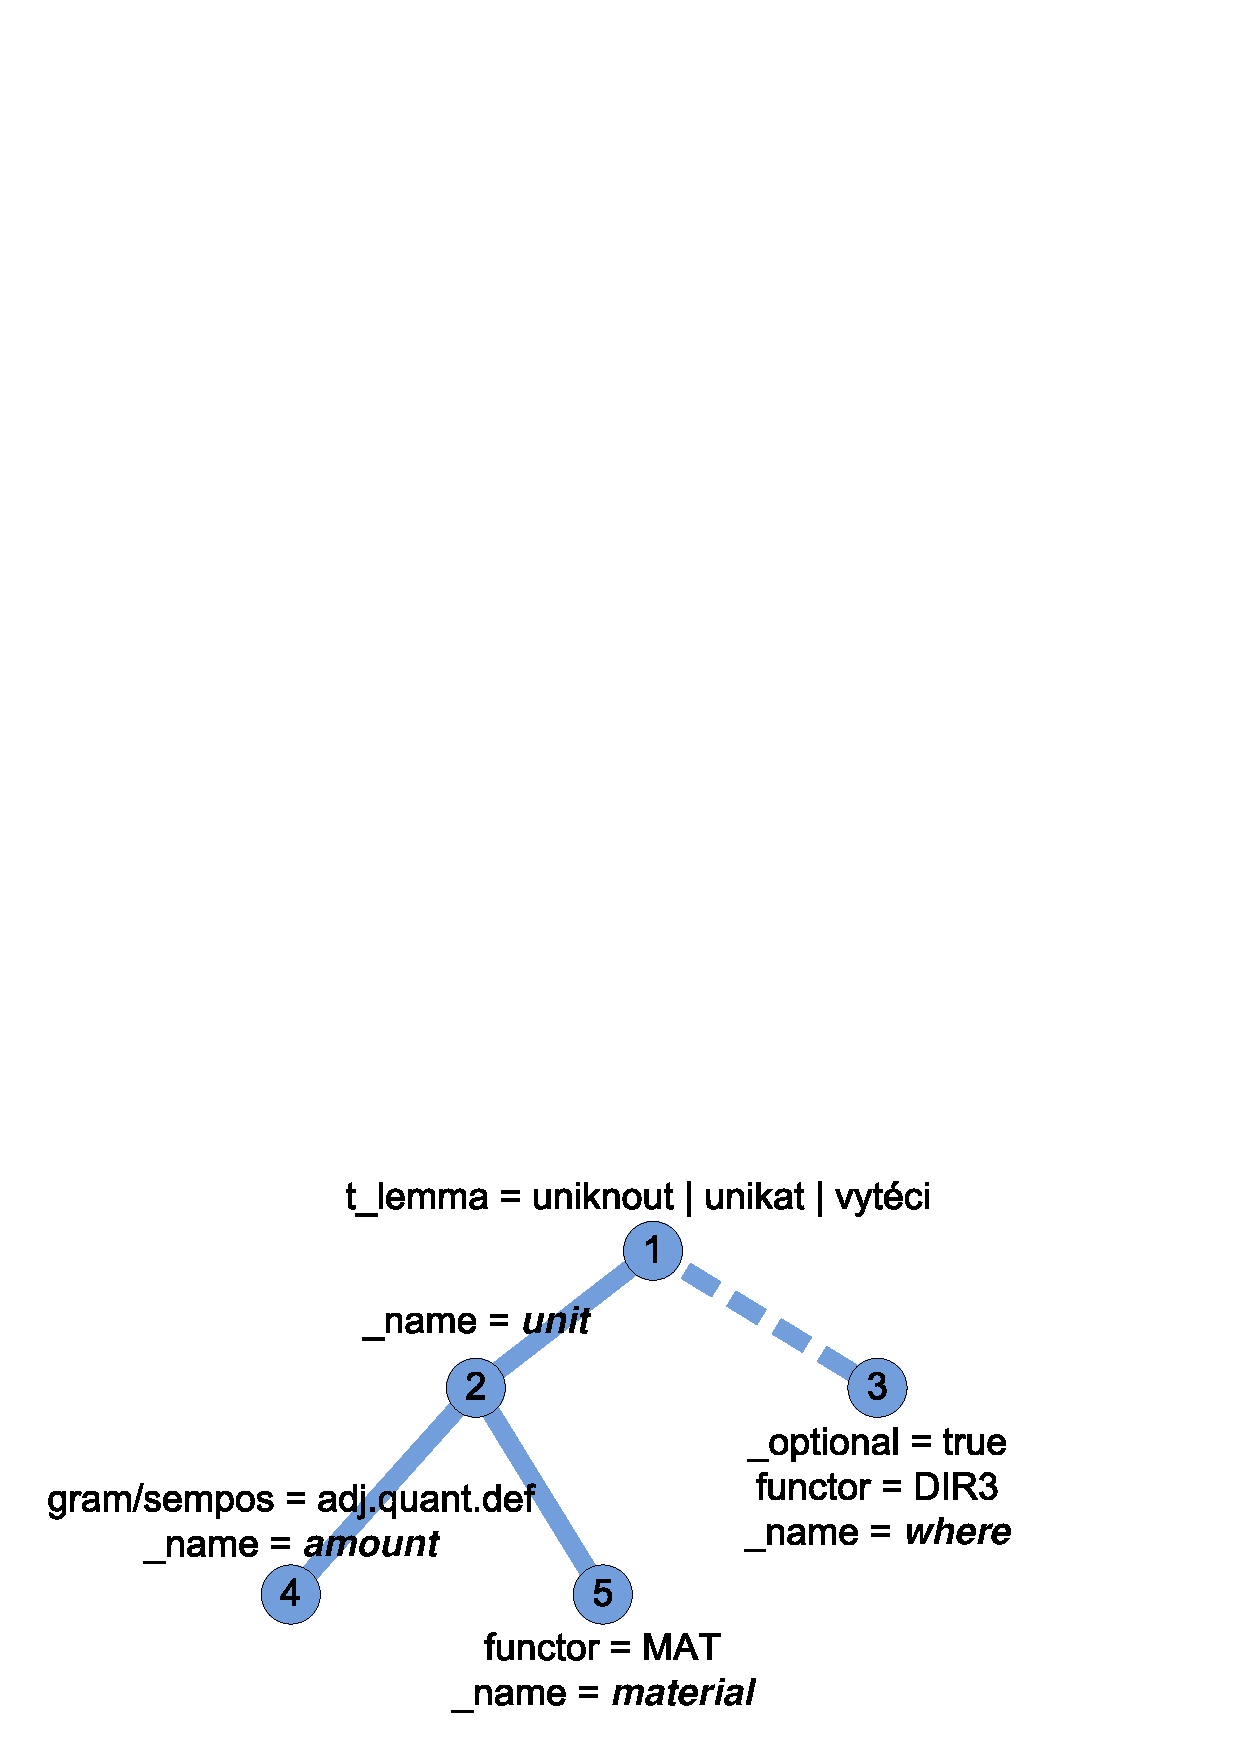
\includegraphics[width=0.5\hsize]{eenv_extract_patern}
\\Transcript:\\
\begin{tabular}{|c|c|}
\hline
uniknout, unikat & vytéci\\
to leak out & to flow out\\
\hline
\end{tabular}		
	\caption{A manually created extraction rule investigating dangerous liquids that spilled out into the environment.}
	\label{fig:manual_eenv_extract_patern}
\end{figure}


\begin{figure}
	\centering
		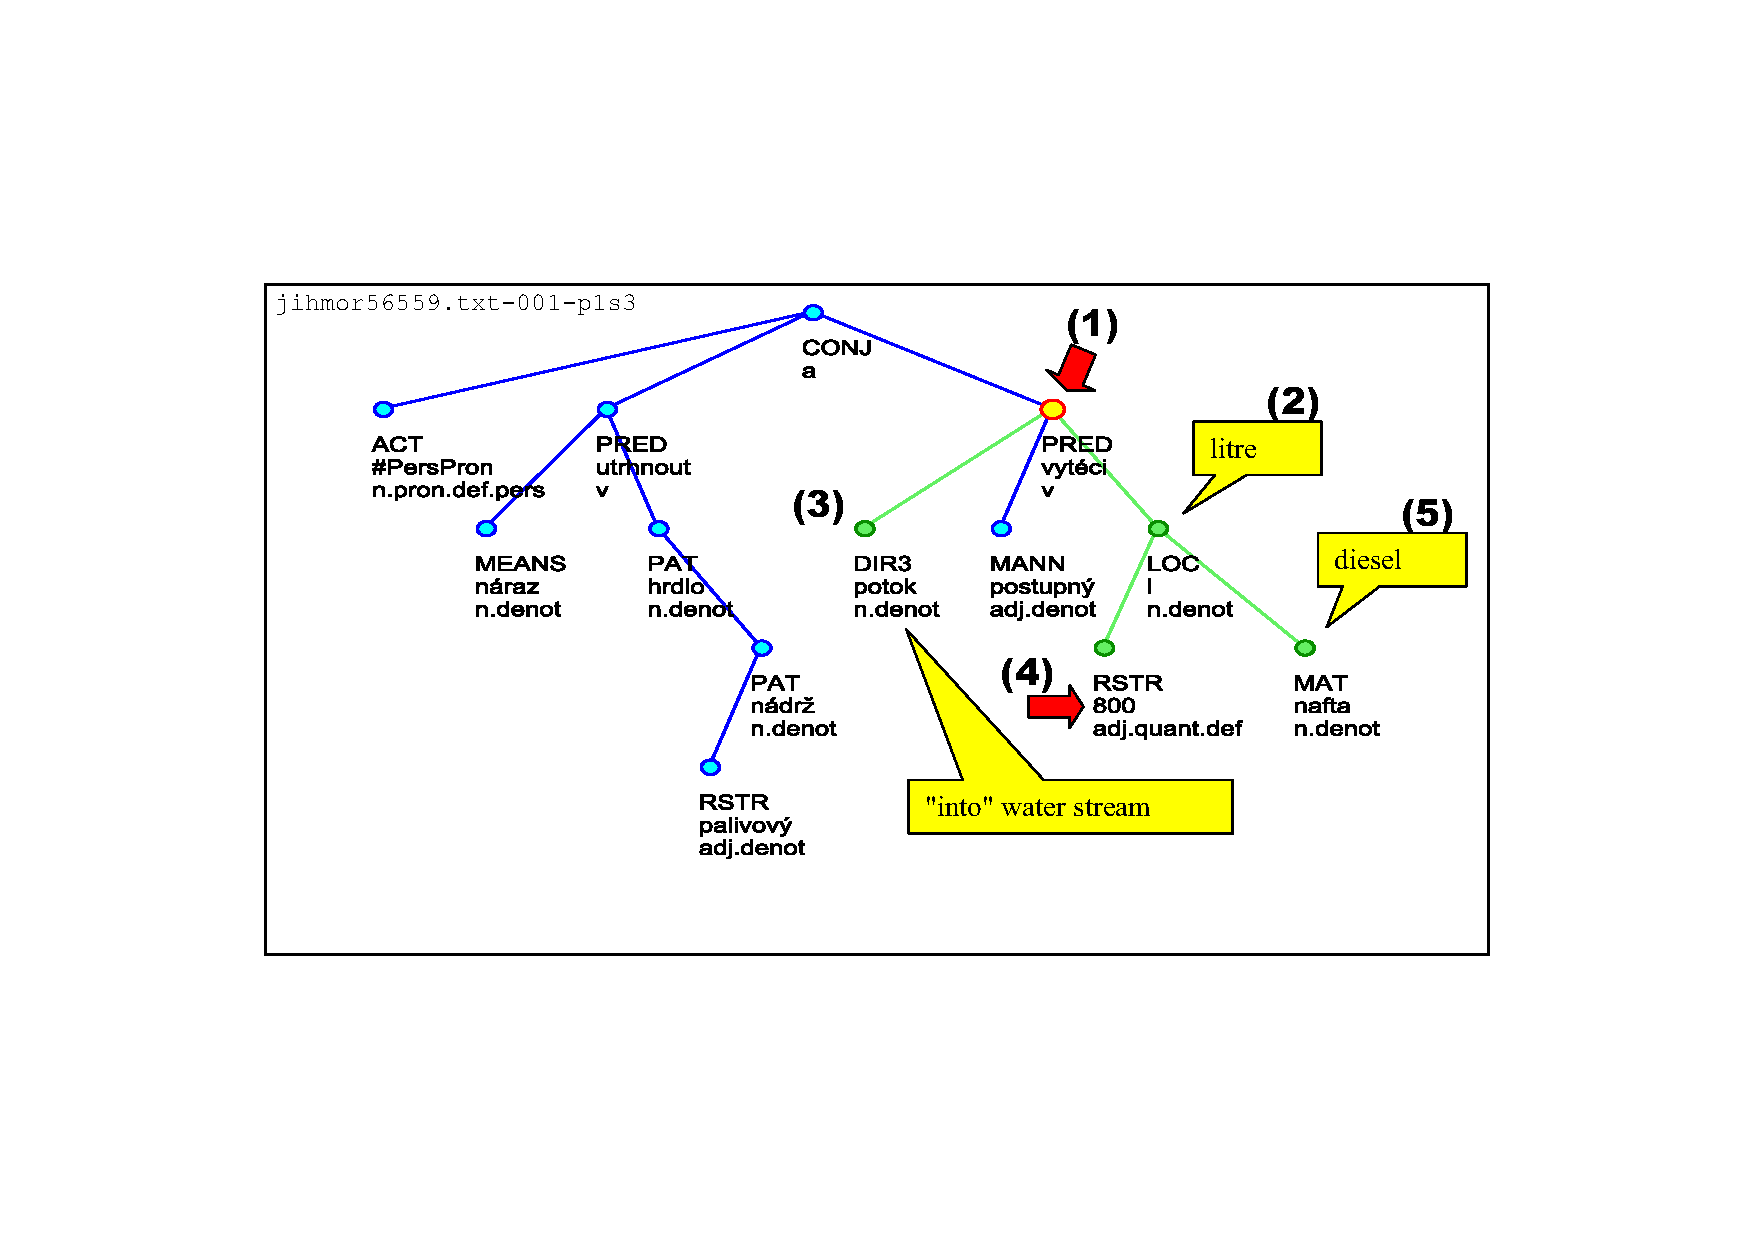
\includegraphics[angle=-90, width=0.6\hsize]{eenv_matching_tree}
		
Original sentence: 
\emph{``Nárazem se utrhl hrdlo palivové nádrže a do potoka postupně vyteklo na 800 litrů nafty.''}\\
English transcript: 
\emph{``Due to the clash the throat of fuel tank tore off and 800 liters of oil (diesel) has run out to a stream.''}
	\caption{A tree matching with the corresponding extraction rule in Figure~\ref{fig:manual_eenv_extract_patern}.}
	\label{fig:manual_eenv_matching_tree}
\end{figure}


%%%%%%%%%%%%%%%%%%%%%%%%%%%%%%%%%%%%%%%%%%%%%%%%%%%%%%%%%%%%%%%%%%%%%%%%%%%%%%%%%%%%%
\begin{figure}
\begin{minted}[linenos,  fontsize=\footnotesize,
               frame=lines, tabsize=2]{xml}
<QueryMatches>
	<Match root_id="T-vysocina63466.txt-001-p1s4" match_string="2:0,7:3,8:4,11:2">
		<Sentence>
			Při požáru byla jedna osoba lehce zraněna - jednalo se
			o majitele domu, který si vykloubil rameno.
		</Sentence>
		<Data>
			<Value variable_name="action_type" attribute_name="t_lemma">zranit</Value>
			<Value variable_name="injury_manner" attribute_name="t_lemma">lehký</Value>
			<Value variable_name="participant" attribute_name="t_lemma">osoba</Value>
			<Value variable_name="quantity" attribute_name="t_lemma">jeden</Value>
		</Data>
	</Match>
	<Match root_id="T-jihomoravsky49640.txt-001-p1s4" match_string="1:0,13:3,14:4">
		<Sentence>
			Ve zdemolovaném trabantu na místě zemřeli dva muži - 82letý senior
			a další muž, jehož totožnost zjišťují policisté.
		</Sentence>
		<Data>
			<Value variable_name="action_type" attribute_name="t_lemma">zemřít</Value>
			<Value variable_name="participant" attribute_name="t_lemma">muž</Value>
			<Value variable_name="quantity" attribute_name="t_lemma">dva</Value>
		</Data>
	</Match>
	<Match root_id="T-jihomoravsky49736.txt-001-p4s3" match_string="1:0,3:3,7:1">
		<Sentence>Čtyřiatřicetiletý řidič nebyl zraněn.</Sentence>
		<Data>
			<Value variable_name="action_type" attribute_name="t_lemma">zranit</Value>
			<Value variable_name="a-negation" 
			       attribute_name="m/tag">VpYS---XR-NA---</Value>
			<Value variable_name="participant" attribute_name="t_lemma">řidič</Value>
		</Data>
	</Match>
</QueryMatches>
\end{minted}
\caption{\emph{XML} structured output of the SQL select like query. A negation can be detected from the presence of \emph{m/tag} on the line 30.}
\label{fig:select_xml}
\end{figure}
%%%%%%%%%%%%%%%%%%%%%%%%%%%%%%%%%%%%%%%%%%%%%%%%%%%%%%%%%%%%%%%%%%%%%%%%%%%%%%%%%%%%%

\begin{figure}
	\centering
		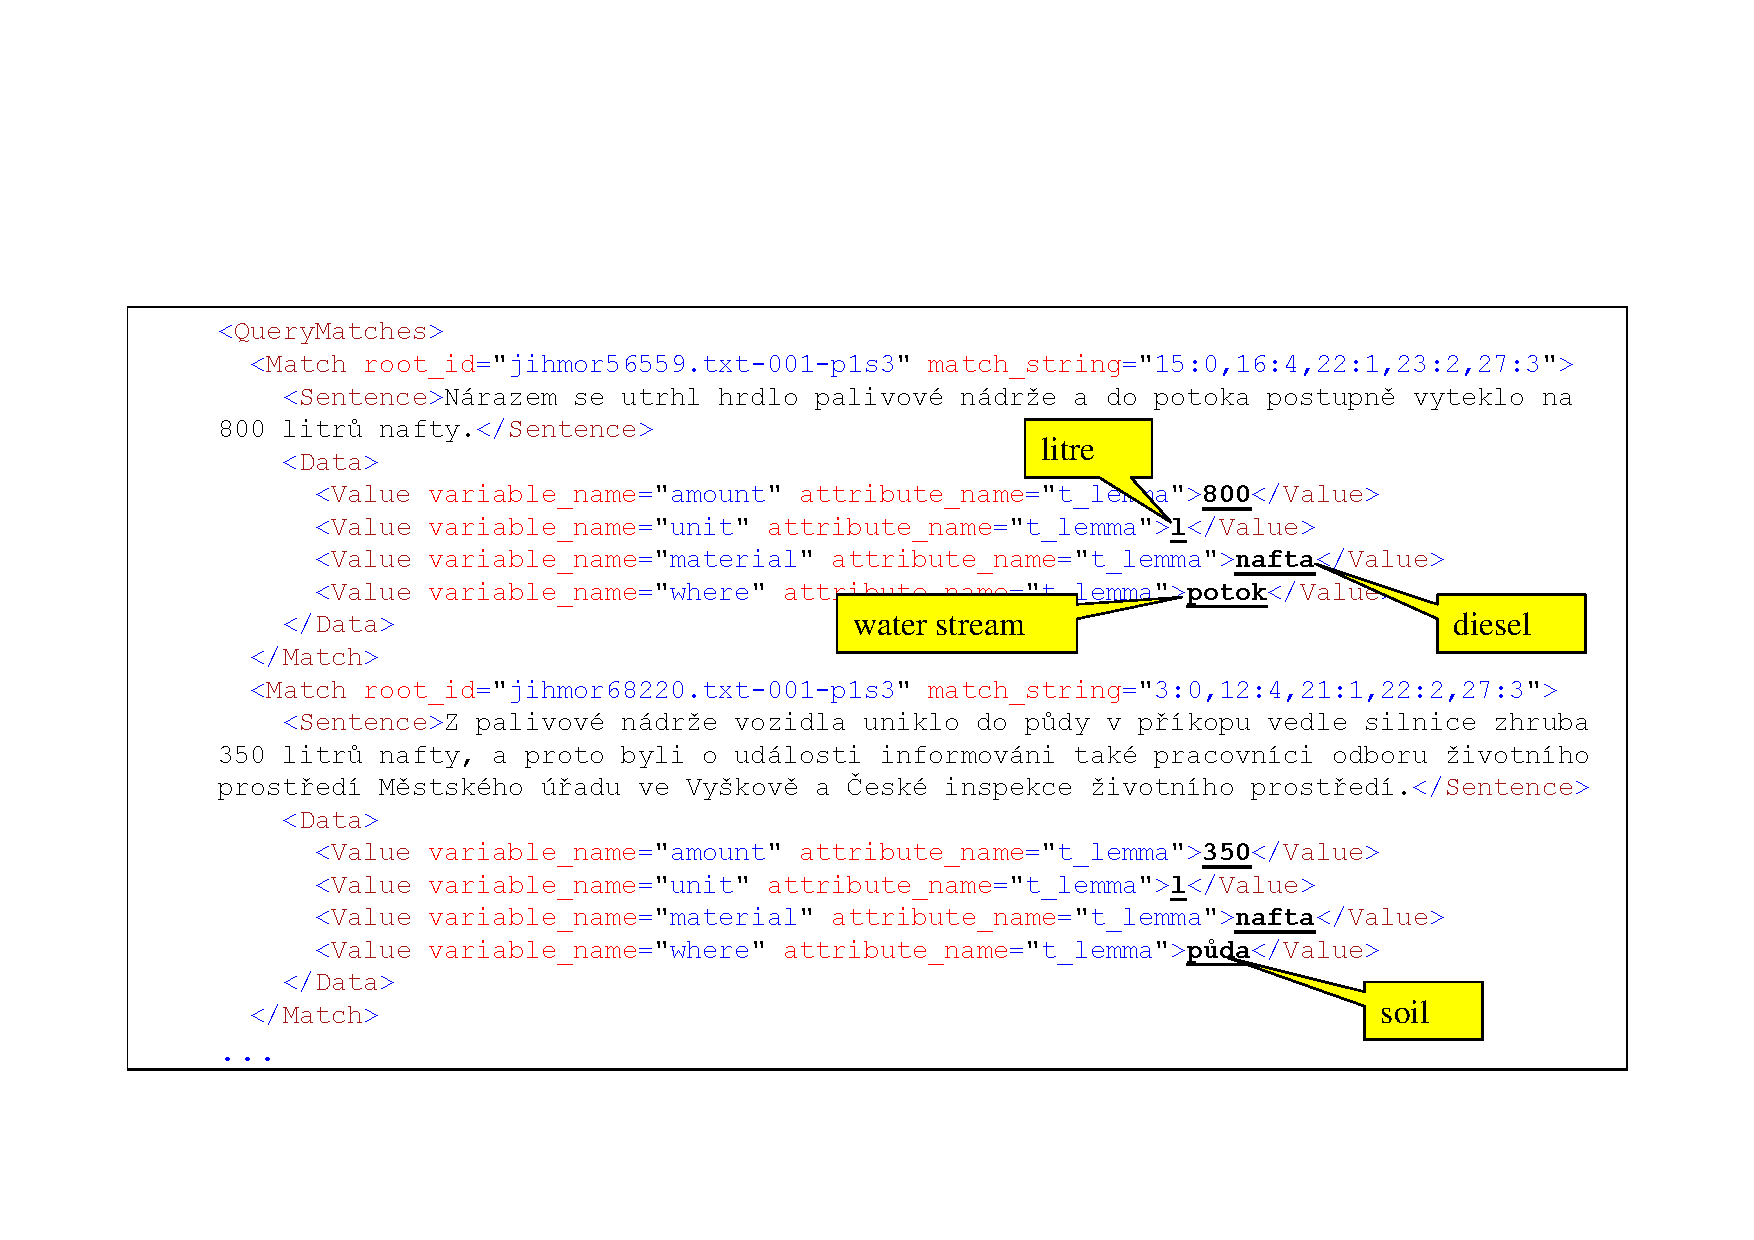
\includegraphics[angle=-90, width=0.7\hsize]{eenv_results}
	\caption{\emph{XML} structured output of the SQL select like query corresponding with the extraction rule in Figure~\ref{fig:manual_eenv_extract_patern} and matching tree in Figure~\ref{fig:manual_eenv_matching_tree}.}
	\label{fig:manual_eenv_results}
\end{figure}























\subsubsection{Illustration Examples}



Evaluation of the extraction rule from Figure~\ref{fig:manual_eenv_extract_patern} is illustrated on Figure~\ref{fig:manual_eenv_matching_tree}. Figure~\ref{fig:manual_eenv_matching_tree} shows a linguistic tree matching with the extraction rule. Matching nodes are decorated and labeled by the numbers of corresponding query nodes.



\subsection{Extraction Output} \label{sec:manual_impl_output}

Small pieces of extraction outputs are shown in Figure~\ref{fig:select_xml} (for the extraction rule in Figure~\ref{fig:manual_extract_patern}) and in Figure~\ref{fig:manual_eenv_results} (for the extraction rule in Figure~\ref{fig:manual_eenv_extract_patern}). 

The former example (Figure~\ref{fig:select_xml}) contains three matches of the extraction rule in three different articles. Each query match is closed in the \verb+<Match>+ element and each contains values of some linguistic attributes closed inside the \verb+<Value>+ elements. Each value comes from some of the nodes of the extraction rule. Name of corresponding query node is saved in the \verb+variable_name+ attribute of the \verb+<Value>+ element.

In the case of the example query, values identified by the variable \verb+action_type+ specify the type of the action. So in the first and third case somebody was injured (\emph{zranit} means to injure in Czech, lines 8 and 28) and in the second case somebody died (\emph{zemřít} means to die in Czech, line 20).

Values identified by \verb+participant+ and \verb+quantity+ contain information about participants of the action. \verb+participant+ serves for specification of the type of the participants and \verb+quantity+ values hold numbers (quantity) of the participants. So in the first action one (\emph{jeden}, line 11) person (\emph{osoba}, line 10) was injured and in the second action two (\emph{dva}, line 22) men (\emph{muž}, line 21) died.

Values identified by \verb+a-negation+ contain the information about a negation of a clause (The presence of negation is indicated by the 11th character of the position-based morphological tag, note that the corresponding node (number 2) of the extraction rule is marked as optional and the restriction on m/tag is put in the form of regular expression on the 11th character.) So we can see that the participant (driver -- \emph{řidič}, line 31) of the last action was \textbf{not} injured (lines 29-30).

The last not described attribute name is \verb+injury_manner+. Corresponding values contain information about the manner of injury of an injury action. So in the first action of the example there was a light injury (\emph{lehký} means light in Czech, line 9).








%%%%%%%%%%%%%%%%%%%%%%%%%%%%%%%%%%%%%%%%%%%%%%%%%%%%%%%%%%%%%%%%%%%%%%%%%%%%%%%%%%%%%
%%%%%%%%%%%%%%%%%%%%%%%%%%%%%%%%%%%%%%%%%%%%%%%%%%%%%%%%%%%%%%%%%%%%%%%%%%%%%%%%%%%%%
\section{Machine Learning of Extraction Rules} \graphicspath{{../img/ch60/}} \label{sec:learning_impl}



Here we just briefly describe implementation of our system. The system consists of several modules, all integrated in GATE as processing resources (PRs).

\subsection{TectoMT Wrapper (Linguistic Analysis)} \label{sec:learning_tectomt_wrapper}

TectoMT wrapper is a GATE component (processing resource), which takes the text of a GATE document, sends it to TectoMT linguistic analyzers, parses the results and converts the results to the form of GATE annotations. The next section provides details about how PDT annotations are represented in GATE.

Because TectoMT has to run as a separate process (it is implemented in Perl) and the initialization of TectoMT analyzers usually takes significant amount of time it would be very inefficient to start a new TectoMT instance for each document. Therefore the implementation currently offers two modes of execution: batch (TectoMTBatchAnalyser) and online (TectoMTOnlineAnalyser).

The batch mode is implemented similarly to the Batch Learning PR\footnote{\url{http://gate.ac.uk/userguide/sec:ml:batch-learning-pr}}. Batch mode of execution in the context of GATE corpus pipelines is a deviation from the standard execution mode, when documents are processed one by one. During the execution as a part of a corpus pipeline, TectoMTBatchAnalyser only accumulates documents and the whole work is done as a batch when the last document is encountered. This also implies that TectoMTBatchAnalyser has to be the last PR in the pipeline because it produces no output in the time of execution (except for the last document when the whole batch is executed). 

Client-server model of implementation is used in the online mode. A separate TectoMT server process is started at the time of initialization and during the execution, GATE documents are processed in ordinary way, one by one. This means that (similarly to the previous case) each document is converted to the TectoMT readable format, sent to TectoMT and the result is converted back to GATE. The online mode of execution is a bit slower than the batch mode because additional time is spent on client-server communication (XML-RPC\footnote{\url{http://www.xmlrpc.com/}}).



\subsection{PDT Annotations in GATE} \label{sec:learning_pdt_in_gate} \label{sec:LDR_in_GATE}

Although GATE annotations are just highlighted pieces of text (see also Section~\ref{sec:third_gate_annotations}) it is possible to use them to encode dependency tree structures. It is possible because each GATE annotation has a unique identifier (ID) and an arbitrary set of features (name-value pairs) can be assigned to it. The way how the PDT dependency trees are encoded in GATE is in fact the same as in the GATE wrapper for the Stanford Parser\footnote{\url{http://gate.ac.uk/userguide/sec:parsers:stanford}}. 

Three main constructs are used to capture an arbitrary configuration of a linguistic dependency tree:


\begin{description}
	\item[tree nodes] (usually corresponding to words (tokens) of a sentence)
	\item[edges] (dependency relations between nodes)
	\item[node attributes] (connected linguistic features like POS, gender, tense, case, etc.)
\end{description}

These constructs are encoded in GATE in the following way: tree nodes correspond to \emph{token} annotations, node attributes are saved as token annotation features and edges are encoded as another special kind of annotations.

Two kinds of token annotations are used to represent two kinds of trees and tree nodes. ``Token'' annotation type is used for analytical tree nodes and ``tToken'' for tectogrammatical tree nodes.

Four kinds of edges (PDT dependencies) are implemented by the TectoMT wrapper: analytical dependencies, tectogrammatical dependencies, aux.rf (auxiliary reference) and lex.rf (main lexical reference). The last two kinds (aux.rf and lex.rf) are used to connect tectogrammatical and analytical nodes. The implementation differs according to the cardinality of a dependency type. The first three kinds are of the cardinality one-to-many (one parent node can have many children nodes) and the last one (lex.rf) if of the cardinality one-to-one (one parent node has at most one child). Because of that, lex.rf edges can be stored as features (with the name ``lex.rf'') of ``tToken'' annotations. Note that a single GATE annotation feature can have at most one value in each annotation. In this case the annotation ID of the referenced ``Token'' annotation (referenced analytical node) is the value of the lex.rf feature.

One-to-many dependencies are stored as separate annotations (type names: ``aDependency'', ``tDependency'', ``aux.rf'') with a single feature called ``args''. Values of this feature are of Java type List<Integer> (list of integers). The list always contains just two items. The first one is the annotation ID of the parent annotation; the second one is the ID of the child annotation. Instead of using one list feature, two simple features (like ``arg1'', ``arg2'' or ``parentID'', ``childID'') could be used, but the implementation is consistent with the wrapper for the Stanford Parser\footnote{\url{http://gate.ac.uk/userguide/sec:parsers:stanford}}, which uses the single list feature called ``args''), thus PDT dependencies are compatible with Stanford dependencies in GATE.

It is not simple to demonstrate the GATE representation of the dependencies in a static printed form; we can only show a GATE screenshot (Figure~\ref{fig:PDT_GATE}) that partly illustrates that.


\begin{figure}
	\centering
		\framebox{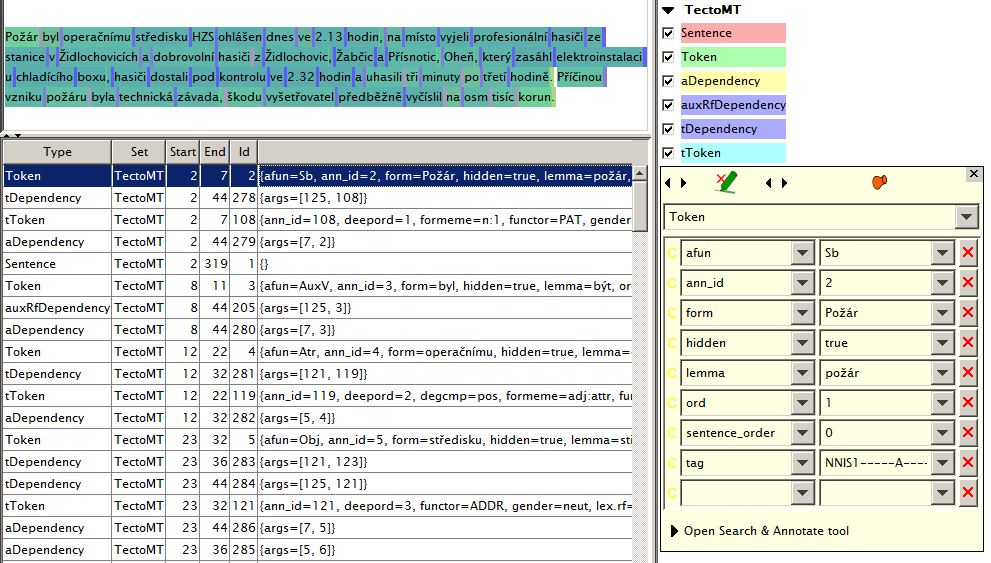
\includegraphics[width=0.7\hsize]{PDT_GATE}}
	\caption{PDT annotations in GATE (screenshot).}
	\label{fig:PDT_GATE}
\end{figure}


\subsubsection{Netgraph Tree Viewer} \label{sec:learning_GATE_Netgraph}

Figure~\ref{fig:GATE_Netgraph}

\begin{figure}
	\centering
		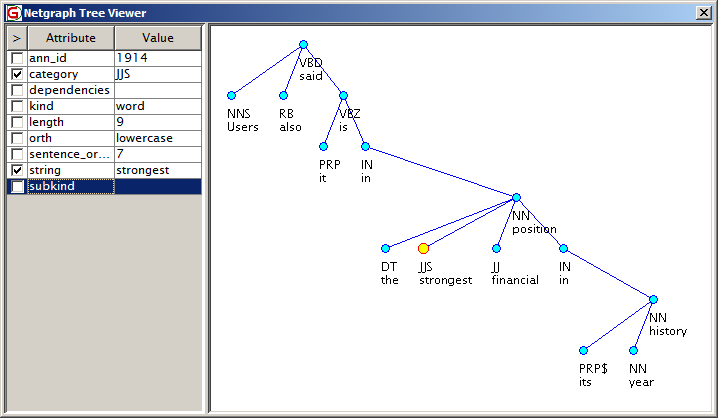
\includegraphics[width=0.7\hsize]{netgraph_stanford}
		\\Sentence: Users also said it is in the strongest financial position in its 24-year history.
	\caption{Netgraph Tree Viewer in GATE (for Stanford Dependencies, screenshot).}
	\label{fig:GATE_Netgraph}
\end{figure}


\subsection{ILP Wrapper (Machine Learning)} \label{sec:learning_ilp_wrapper}
After a human annotator have annotated several documents with desired target annotations, machine learning takes place. 
This consists of two steps: 
\begin{enumerate}
	\item learning of extraction rules from the target annotations and
	\item application of the extraction rules on new documents.
\end{enumerate}
In both steps the linguistic analysis has to be done before and in both steps ILP background knowledge (a logical database of facts) is constructed from linguistic structures of documents that are being processed. We call the process of background knowledge construction as \emph{ILP serialization}; more details are presented below in Section~\ref{sec:learning_ilp_serialization}.

After the ILP serialization is done, the next step depends on the phase which is being performed.

In the learning case, positive and negative examples are constructed from target annotations and the machine learning ILP inductive procedure is executed to obtain extraction rules.

In the application case a Prolog system is used to check if the extraction rules entail any of target annotation candidates.


%Learning / application
%\\1.	serialization -> learning in ILP
%\\2.	serialization -> application in ILP


The learning examples and annotation candidates are usually constructed from all document tokens (and we did so in the present solution), but it can be optionally changed to any other textual unit, for example only numerals or tectogrammatical nodes (words with lexical meaning) can be selected. This can be done easily with the help of \emph{Machine Learning PR} (LM PR) from GATE\footnote{\emph{Machine Learning PR} is an old GATE interface for ML and it is almost obsolete but in contrast to the new \emph{Batch Learning PR} the LM PR is easy to extend for a new ML engine.}.

ML PR provides an interface for exchange of features (including target class) between annotated texts and propositional learners in both directions -- during learning as well as during application. We have used ML PR and developed our \emph{ILP Wrapper} for it. The implementation was a little complicated because complex linguistic structures cannot be easily passed as propositional features, so in our solution we use the ML PR interface only for exchange of the class attribute and annotation id and we access the linguistic structures directly in a document.



\subsection{ILP Serialization} \label{sec:learning_ilp_serialization}

In this section details about conversion of linguistic trees to ILP background knowledge (a Prolog logical database of facts) will be presented. Although the construction is quite strait forward it is worth describing because it makes it easier to understand the extraction rules found by the ILP learning procedure. 

As mentioned in Section~\ref{sec:learning_pdt_in_gate}: three main constructs are used to capture an arbitrary configuration of a dependency linguistic tree: nodes, edges and node attributes. During the process of ILP Serialization these constructs are rendered to Prolog in following way. 

A unique identifier (node ID) is generated for every tree node. The identifier is based on document name and GATE annotation ID.\footnote{Note that node IDs based on sentence order and node deep order are used outside of GATE, see PML$\rightarrow$RDF transformation in Section~\ref{sec:onto_pml_to_rdf}.} These node IDs correspond to simple Prolog atoms and they represent tree nodes in the Prolog fact database. A node type (used by the ILP learning algorithm) is assigned to a node ID by predicates \texttt{Token(NodeID)} for analytical tree nodes and \texttt{tToken(NodeID)} for tectogrammatical tree nodes.

Tree nodes are connected by edges using several binary predicates with a common form:

\texttt{dependency\_type\_name(ParentNodeID, ChildNodeID)}

\noindent Note that the parent (governor) node always occupies the first argument and the child (dependant) node the second one. Predicate name \emph{tDependency} is used for tectogrammatical dependencies and \emph{aDependency} for analytical ones. There are also special kinds of dependencies that connect tectogrammatical and analytical nodes: \emph{lex.rf} (main lexical reference) and \emph{aux.rf} (auxiliary reference), in these cases tectogrammatical node occupies the first argument and analytical the second.

Node attributes are assigned to node IDs by binary predicates of the form:

\texttt{attribute\_name(NodeID, AttributeValue)}

\noindent There are about thirty such predicates like \emph{t\_lemma} (tectogrammatical lemma), \emph{functor} (tectogrammatical functor), \emph{sempos} (semantic part of speech), \emph{negation}, \emph{gender}, etc. but only some of them can be found in example extraction rules and we also excluded some of the attributes from serialization examples for space and simplicity reasons.

Example of a serialized tectogrammatical tree is in Figure~\ref{fig:ilp_serialization} it is the same tree as in Figure~\ref{fig:intro_damage_tree}.

\subsubsection{Attachment of Other GATE Annotations}
During the development of the method, it turned out that it would be very useful to attach additional information, represented by overlapping GATE annotations, to tree nodes. This allows combination of information provided by linguistic trees with information provided by other GATE tools like gazetteers, etc. 

Technically, this is realized using binary predicates with a common form:

\texttt{overlap\_OverlappingType\_OverlappedType(}
\\ \phantom{a} \hfill{} \phantom{b} \texttt{OverlappingNodeID, OverlappedNodeID)}

\noindent Overlap with named entities discovers by gazetteers is the most common form of such overlap. For tectogrammatical nodes, it has the form of \texttt{overlap\_Lookup\_tToken(id1,id2)}. An example can be found in Figure~\ref{fig:learning_eval_rules} on line 34. 


%%%%%%%%%%%%%%%%%%%%%%%%%%%%%%%%%%%%%%%%%%%%%%%%%%%%%%%%%%%%%%%%%%%%%%%%%%%%%%%%%%%%%
\begin{figure}
\begin{minted}[linenos, fontsize=\footnotesize,
               frame=lines]{prolog}
tToken(  id_jihomoravsky47443_243).
t_lemma( id_jihomoravsky47443_243, 'být'). %to be
functor( id_jihomoravsky47443_243, 'PRED').
sempos(  id_jihomoravsky47443_243, 'v').
tDependency( id_jihomoravsky47443_243, id_jihomoravsky47443_238).
tToken(  id_jihomoravsky47443_238).
t_lemma( id_jihomoravsky47443_238, ','). %comma
functor( id_jihomoravsky47443_238, 'APPS').
sempos(  id_jihomoravsky47443_238, 'n.denot').
gender(  id_jihomoravsky47443_238, 'nr').
tDependency( id_jihomoravsky47443_238, id_jihomoravsky47443_237).
tToken(  id_jihomoravsky47443_237).
t_lemma( id_jihomoravsky47443_237, 'vyčíslit'). %to quantify
functor( id_jihomoravsky47443_237, 'PAT').
sempos(  id_jihomoravsky47443_237, 'v').
tDependency( id_jihomoravsky47443_237, id_jihomoravsky47443_245).
tToken(  id_jihomoravsky47443_245).
t_lemma( id_jihomoravsky47443_245, 'předběžně'). %preliminarily
functor( id_jihomoravsky47443_245, 'MANN').
sempos(  id_jihomoravsky47443_245, 'adv.denot.grad.nneg').
tDependency( id_jihomoravsky47443_237, id_jihomoravsky47443_244).
tToken(  id_jihomoravsky47443_244).
t_lemma( id_jihomoravsky47443_244, 'vyšetřovatel'). %investigator
functor( id_jihomoravsky47443_244, 'ACT').
sempos(  id_jihomoravsky47443_244, 'n.denot').
gender(  id_jihomoravsky47443_244, 'anim').
tDependency( id_jihomoravsky47443_237, id_jihomoravsky47443_240).
tToken(  id_jihomoravsky47443_240).
t_lemma( id_jihomoravsky47443_240, 'osm'). %eight
functor( id_jihomoravsky47443_240, 'PAT').
sempos(  id_jihomoravsky47443_240, 'n.quant.def').
gender(  id_jihomoravsky47443_240, 'nr').
tDependency( id_jihomoravsky47443_240, id_jihomoravsky47443_242).
tToken(  id_jihomoravsky47443_242).
t_lemma( id_jihomoravsky47443_242, 'tisíc'). %thousand
functor( id_jihomoravsky47443_242, 'RSTR').
sempos(  id_jihomoravsky47443_242, 'n.quant.def').
gender(  id_jihomoravsky47443_242, 'inan').
tDependency( id_jihomoravsky47443_242, id_jihomoravsky47443_247).
tToken(  id_jihomoravsky47443_247).
t_lemma( id_jihomoravsky47443_247, 'koruna'). %crown
functor( id_jihomoravsky47443_247, 'MAT').
sempos(  id_jihomoravsky47443_247, 'n.denot').
gender(  id_jihomoravsky47443_247, 'fem').
tDependency( id_jihomoravsky47443_237, id_jihomoravsky47443_246).
tToken(  id_jihomoravsky47443_246).
t_lemma( id_jihomoravsky47443_246, 'škoda'). %damage
functor( id_jihomoravsky47443_246, 'PAT').
sempos(  id_jihomoravsky47443_246, 'n.denot').
gender(  id_jihomoravsky47443_246,'fem').
\end{minted}
\caption{ILP serialization example based on the tree from Figure~\ref{fig:intro_damage_tree}.}
\label{fig:ilp_serialization}
\end{figure}
%%%%%%%%%%%%%%%%%%%%%%%%%%%%%%%%%%%%%%%%%%%%%%%%%%%%%%%%%%%%%%%%%%%%%%%%%%%%%%%%%%%%%








\clearpage


%%%%%%%%%%%%%%%%%%%%%%%%%%%%%%%%%%%%%%%%%%%%%%%%%%%%%%%%%%%%%%%%%%%%%%%%%%%%%%%%%%%%%
%%%%%%%%%%%%%%%%%%%%%%%%%%%%%%%%%%%%%%%%%%%%%%%%%%%%%%%%%%%%%%%%%%%%%%%%%%%%%%%%%%%%%
%%%%%%%%%%%%%%%%%%%%%%%%%%%%%%%%%%%%%%%%%%%%%%%%%%%%%%%%%%%%%%%%%%%%%%%%%%%%%%%%%%%%%
\section{Shareable Extraction Ontologies} \label{sec:onto_implement}
\graphicspath{{../img/ch70/}}


In this section we will present details about the implementation of our case study with shareable extraction ontologies.  We have used our IE engine based on deep linguistic parsing and Inductive Logic Programming, which was described in Section~\ref{sec:learning_methods}. It is a complex system implemented with a great help of the GATE system and it also uses many other third party tools including several linguistic tools and a Prolog system. Installation and making the system operate is not simple. This case study should demonstrate that the extraction rules produced by the system are not dependent on the system in the sense of shareable extraction ontologies.




\subsection{Linguistic Analysis}



The IE engine needs a linguistic preprocessing (deep linguistic parsing) of documents on its input. Deep linguistic parsing brings a very complex structure to the text and the structure serves as a footing for the construction and application of extraction rules. We usually use TectoMT system to do the linguistic preprocessing, see Section~\ref{sec:third_tectomt} for details. The output linguistic annotations of the TectoMT system are stored (along with the text of the source document) in XML files in so called Prague Markup Language (PML). PML is a very complex language (or XML schema) that is able to express many linguistic elements and features present in text. For the IE engine a tree dependency structure of words in sentences is the most useful one because the edges of the structure guide the extraction rules. Such (tectogrammatical) tree structure was already presented in this thesis, e.g. in Figure~\ref{fig:intro_damage_tree}.


\subsection{Data Transformation (PML to RDF)} \label{sec:onto_pml_to_rdf}

In this case study, PML files made by TectoMT from source documents are transformed to RDF document ontologies by quite simple GRDDL/XSLT transformation\footnote{The transformation is available on-line at \url{http://czsem.berlios.de/ontologies/tmt2rdf.xsl}}. Such document ontology contains the whole variety of PML in RDF format. An example of such document ontology can be seen in Figure~\ref{fig:rdf_serialization}. It shows RDF serialization of the tree presented in Figure~\ref{fig:intro_damage_tree} and transformed to ILP background knowledge in Figure~\ref{fig:ilp_serialization}. Transcript of Czech words is provided in comments.

Figure~\ref{fig:annotated_DO} shows an example of annotated document ontology, which was created by the application of extraction rules on the document ontology from Figure~\ref{fig:rdf_serialization}. Lines 13-15 and 23-25 are added by reasoner; lines 13-15 and 23 are not very interesting, they show some technical constructions based on the schema mapping, but lines 24 and 25 represent the result of extraction rules, these lines mark the corresponding tree node as ``\emph{mention root} of the \emph{damage} task''. The same annotated document ontology is shown on Figure~\ref{fig:PDT_PROTEGE} as a screenshot of the Protégé ontology editor\footnote{\url{http://protege.stanford.edu/}}.



%%%%%%%%%%%%%%%%%%%%%%%%%%%%%%%%%%%%%%%%%%%%%%%%%%%%%%%%%%%%%%%%%%%%%%%%%%%%%%%%%%%%%
\begin{figure}
\begin{minted}[linenos, fontsize=\footnotesize,
               frame=lines, tabsize=2]{turtle}
@prefix node: <http://czsem.berlios.de/ontolog.../jihomoravsky47443.owl#node/> .
@prefix pml: <http://ufal.mff.cuni.cz/pdt/pml/> .

node:SCzechT-s4-n1 rdf:type pml:Node, owl:Thing;
			pml:t_lemma "být" ; #to be
			pml:sempos "v" ; pml:verbmod "ind" ; 
			pml:lex.rf node:SCzechA-s4-w4 ; pml:hasParent node:SCzechT-s4-root .
node:SCzechT-s4-n10 rdf:type pml:Node, owl:Thing;
			pml:t_lemma "vyšetřovatel" ; #investigator
			pml:negation "neg0" ; pml:sempos "n.denot" ;
			pml:gender "anim" ; pml:number "sg" ;
			pml:formeme "n:1" ; pml:functor "ACT" ;
			pml:lex.rf node:SCzechA-s4-w9 ; pml:hasParent node:SCzechT-s4-n8 .
node:SCzechT-s4-n11 rdf:type pml:Node, owl:Thing;
			pml:degcmp "pos" ; pml:t_lemma "předběžně" ; #preliminarily
			pml:formeme "adv:" ; pml:sempos "adv.denot.grad.nneg" ;
			pml:functor "MANN" ; pml:negation "neg0" ;
			pml:lex.rf node:SCzechA-s4-w10 ; pml:hasParent node:SCzechT-s4-n8 .
node:SCzechT-s4-n12 rdf:type pml:Node, owl:Thing;
			pml:t_lemma "osm" ; #eight
			pml:number "pl" ; pml:numertype "basic" ;
			pml:sempos "n.quant.def" ; pml:formeme "n:???" ;
			pml:functor "PAT" ; pml:gender "nr" ;
			pml:lex.rf node:SCzechA-s4-w13 ; pml:hasParent node:SCzechT-s4-n8 .
node:SCzechT-s4-n13 rdf:type pml:Node, owl:Thing;
			pml:t_lemma "tisíc" ; #thousand
			pml:number "sg" ; pml:functor "RSTR" ;
			pml:gender "inan" ; pml:sempos "n.quant.def" ;
			pml:numertype "basic" ; pml:formeme "n:???" ;
			pml:lex.rf node:SCzechA-s4-w14 ; pml:hasParent node:SCzechT-s4-n12 .
node:SCzechT-s4-n14 rdf:type pml:Node, owl:Thing;
			pml:t_lemma "koruna" ; #crown
			pml:gender "fem" ; pml:sempos "n.denot" ;
			pml:number "pl" ; pml:formeme "n:2" ;
			pml:functor "MAT" ; pml:negation "neg0" ;
			pml:lex.rf node:SCzechA-s4-w15 ; pml:hasParent node:SCzechT-s4-n13 .
node:SCzechT-s4-n7 rdf:type pml:Node, owl:Thing;
			pml:t_lemma "," ; #comma
			pml:gender "nr" ; pml:negation "neg0" ;
			pml:sempos "n.denot" ; pml:functor "APPS" ;
			pml:formeme "n:???" ; pml:number "nr" ;
			pml:lex.rf node:SCzechA-s4-w7 ; pml:hasParent node:SCzechT-s4-n1 .
node:SCzechT-s4-n8 rdf:type pml:Node, owl:Thing;
			pml:t_lemma "vyčíslit" ; #quantify
			pml:is_member "1" ; pml:deontmod "decl" ; pml:formeme "v:fin" ;
			pml:tense "ant" ; pml:verbmod "ind" ; pml:aspect "cpl" ;
			pml:is_clause_head "1" ; pml:functor "PAR" ;
			pml:dispmod "disp0" ; pml:sempos "v" ; pml:negation "neg0" ;
			pml:lex.rf node:SCzechA-s4-w11 ; pml:hasParent node:SCzechT-s4-n7 .
node:SCzechT-s4-n9 rdf:type pml:Node, owl:Thing;
			pml:t_lemma "škoda" ; #damage
			pml:sempos "n.denot" ; pml:functor "PAT" ; pml:gender "fem" ;
			pml:formeme "n:4" ; pml:number "sg" ; pml:negation "neg0" ;
			pml:lex.rf node:SCzechA-s4-w8 ; pml:hasParent node:SCzechT-s4-n8 .
\end{minted}
\caption{Document ontology (RDF serialization of linguistic trees), based on Figure~\ref{fig:intro_damage_tree}}.
\label{fig:rdf_serialization}
\end{figure}
%%%%%%%%%%%%%%%%%%%%%%%%%%%%%%%%%%%%%%%%%%%%%%%%%%%%%%%%%%%%%%%%%%%%%%%%%%%%%%%%%%%%%




%%%%%%%%%%%%%%%%%%%%%%%%%%%%%%%%%%%%%%%%%%%%%%%%%%%%%%%%%%%%%%%%%%%%%%%%%%%%%%%%%%%%%
\begin{figure}
\begin{minted}[linenos, fontsize=\footnotesize,
               frame=lines, tabsize=2]{turtle}
@prefix node: <http://czsem.berlios.de/ontologies/.../jihomoravsky47443.owl#node/> .
@prefix pml: <http://ufal.mff.cuni.cz/pdt/pml/> .
# Mapping Ontology
@prefix PML2GATE: <http://czsem.berlios.de/ontologies/PML2GATE_ontology_utils.owl#> .

node:SCzechT-s4-n12 rdf:type pml:Node, owl:Thing;
			 pml:t_lemma "osm" ; #eight
			 pml:number "pl" ; pml:numertype "basic" ;
			 pml:sempos "n.quant.def" ; pml:formeme "n:???" ;
			 pml:functor "PAT" ; pml:gender "nr" ;
			 pml:lex.rf node:SCzechA-s4-w13 ; pml:hasParent node:SCzechT-s4-n8 ;
################### Added by Reasoner ############################################
			 rdf:type PML2GATE:TNode ; #Tectogrammatical node
			 PML2GATE:hasChild node:SCzechT-s4-n13 ;
			 pml:tDependency node:SCzechT-s4-n13 .
##################################################################################
node:SCzechA-s4-w13 rdf:type pml:Node, owl:Thing;
			 pml:is_auxiliary "0" ; pml:edge_to_collapse "1" ;
			 pml:ord "13" ; pml:tag "Cn-S4----------" ;
			 pml:afun "Obj" ; pml:form "osm" ; pml:lemma "osm\1408" ;
			 pml:m.rf node:SCzechM-s4-w13 ; pml:hasParent node:SCzechA-s4-w12 ;
################### Added by Reasoner ############################################
			 PML2GATE:hasChild node:SCzechA-s4-w14 ;
			 pml:mention_root "damage" ;
			 rdf:type PML2GATE:MentionRoot .
##################################################################################
\end{minted}
\caption{Annotated document ontology example}
\label{fig:annotated_DO}
\end{figure}
%%%%%%%%%%%%%%%%%%%%%%%%%%%%%%%%%%%%%%%%%%%%%%%%%%%%%%%%%%%%%%%%%%%%%%%%%%%%%%%%%%%%%

\begin{figure}
\centerline{\framebox{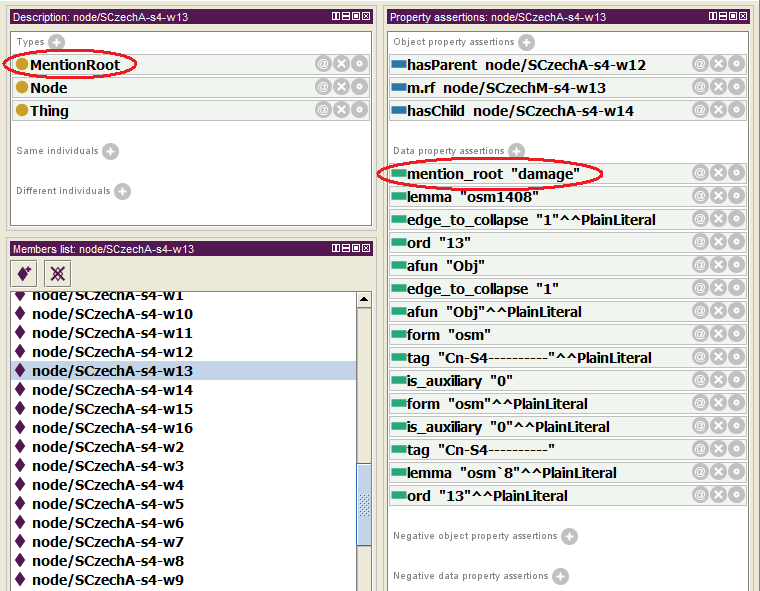
\includegraphics[width=0.7\hsize]{PDT_PROTEGE.png}}}
\caption{Annotated document ontology in Protégé ontology editor}
\label{fig:PDT_PROTEGE}
\end{figure}






\clearpage

\subsection{Rule Transformations}


Extraction rules produced by the IE engine are natively kept in a Prolog format; examples can be seen in Figure~\ref{fig:rules_prolog}. The engine is capable to export them to the OWL/XML\footnote{\url{http://www.w3.org/TR/owl-xmlsyntax/}} syntax for rules in OWL 2 \citep{GHPP09a} (see in Figure~\ref{fig:rules_xml}). Such rules can be parsed by OWL API\footnote{\url{http://owlapi.sourceforge.net/}} 3.1 
and exported to RDF/SWRL, which is very widely supported and hopefully becoming a W3C recommendation.
Figure~\ref{fig:rules_protege} shows the example rules in Prot\'{e}g\'{e} 4 -- Rules View's format. The last rule example can be seen in Figure~\ref{fig:rules_jena}, it shows a rule in the Jena rules format\footnote{\url{http://jena.sourceforge.net/inference/#RULEsyntax}}. Conversion to Jena rules was necessary because it is the only format that Jena can parse, see details about our use of Jena in Section~\ref{sec:onto_experiment}. The Jena rules were obtained using following transformation process:
\begin{enumerate}
	\item OWL/XML $\rightarrow$ RDF/SWRL conversion using OWL API and 
	\item RDF/SWRL $\rightarrow$ Jena rules conversion using SweetRules\footnote{\url{http://sweetrules.semwebcentral.org/}}.
\end{enumerate}


The presented rules belong to the group of so called DL-Safe rules \citep{Motik:DL-Safe-rules} so the decidability of OWL reasoning is kept.




\begin{figure}
\begin{minted}[linenos,  fontsize=\footnotesize,
               frame=lines, tabsize=2]{prolog}
%[Rule 1] [Pos cover = 14 Neg cover = 0]
mention_root(damage,A) :-
   'lex.rf'(B,A), sempos(B,'n.quant.def'), tDependency(C,B), tDependency(C,D), 
   t_lemma(D,'vyšetřovatel'). %investigator

%[Rule 2] [Pos cover = 13 Neg cover = 0]
mention_root(damage,A) :-
   'lex.rf'(B,A), functor(B,'TOWH'), tDependency(C,B), tDependency(C,D), 
   t_lemma(D,'škoda'). %damage
\end{minted}
	\caption{Examples of extraction rules in the native Prolog format.}
	\label{fig:rules_prolog}
\end{figure}


\begin{figure}
\begin{minted}[linenos,  fontsize=\footnotesize,
               frame=lines, tabsize=2]{xml}
<?xml version="1.0" encoding="UTF-8"?>
<!DOCTYPE Ontology [
	<!ENTITY pml "http://ufal.mff.cuni.cz/pdt/pml/" >
]>
<Ontology xmlns="http://www.w3.org/2002/07/owl#"
	ontologyIRI="http://czsem.berlios.de/ontologies/...rules.owl">
	<DLSafeRule>
		<Body>
			<ObjectPropertyAtom> <ObjectProperty IRI="&pml;lex.rf"/>
				<Variable IRI="urn:swrl#b"/> <Variable IRI="urn:swrl#a"/>
			</ObjectPropertyAtom>
			<DataPropertyAtom> <DataProperty IRI="&pml;sempos"/>
				<Variable IRI="urn:swrl#b"/> <Literal>n.quant.def</Literal>
			</DataPropertyAtom>
			<ObjectPropertyAtom> <ObjectProperty IRI="&pml;tDependency"/>
				<Variable IRI="urn:swrl#c"/> <Variable IRI="urn:swrl#b"/>
			</ObjectPropertyAtom>
			<ObjectPropertyAtom> <ObjectProperty IRI="&pml;tDependency"/>
				<Variable IRI="urn:swrl#c"/> <Variable IRI="urn:swrl#d"/>
			</ObjectPropertyAtom>
			<DataPropertyAtom> <DataProperty IRI="&pml;t_lemma"/>
				<Variable IRI="urn:swrl#d"/> <Literal>vyšetřovatel</Literal>
			</DataPropertyAtom>
		</Body>
		<Head>
			<DataPropertyAtom> <DataProperty IRI="&pml;mention_root" />
				<Literal>damage</Literal> <Variable IRI="urn:swrl#a" />
			</DataPropertyAtom>
		</Head>
	</DLSafeRule>
</Ontology>
\end{minted}
\caption{Rule 1 in the OWL/XML syntax for Rules in OWL 2 \citep{GHPP09a}.}
\label{fig:rules_xml}
\end{figure}


\begin{figure}
\begin{minted}[linenos,  fontsize=\footnotesize,
               frame=lines, tabsize=2]{jena}
#[Rule 1]
lex.rf(?b, ?a), sempos(?b, "n.quant.def"), tDependency(?c, ?b),
tDependency(?c, ?d), t_lemma(?d, "vyšetřovatel") #investigator
		-> mention_root(?a, "damage")

#[Rule 2]
lex.rf(?b, ?a), functor(?b, "TOWH"), tDependency(?c, ?b),
tDependency(?c, ?d), t_lemma(?d, "škoda") #damage
		-> mention_root(?a, "damage")
\end{minted}
	\caption{Examples of extraction rules in Prot\'{e}g\'{e} 4 -- Rules View's format.}
	\label{fig:rules_protege}
\end{figure}



\begin{figure}
\begin{minted}[linenos,  fontsize=\footnotesize,
               frame=lines, tabsize=2]{jena}
@prefix pml: <http://ufal.mff.cuni.cz/pdt/pml/>.
[rule-75:  
        ( ?b pml:lex.rf ?a )
        ( ?b pml:sempos 'n.quant.def' )
        ( ?c pml:tDependency ?b )
        ( ?c pml:tDependency ?d )
        ( ?d pml:t_lemma 'vyšetřovatel' )
     -> 
        ( ?a pml:mention_root 'damage' )
]
\end{minted}
\caption{Rule 1 in the Jena rules syntax.}
\label{fig:rules_jena}
\end{figure}


\clearpage










\section{Fuzzy ILP Classification}

In the experimental system we use two inductive logic approaches: crisp and fuzzy (as described above). Technically, the difference between the approaches consists in a different setting of the underlying \emph{ILP task}. Both can be done with a classical ILP tool (Aleph (see Section~\ref{sec:third_ILP_tool}) was used in the final implementation).

We have compared results of the crisp and fuzzy approaches with other classification methods and, in our experiment, the fuzzy approach produced better results than many other methods, including the crisp one. See Section~\ref{sec:fuzzy_results} for details.



\begin{figure}
\begin{minipage}[b]{0.5\hsize}
\begin{minted}[mathescape,fontsize=\footnotesize,
               frame=single]{prolog}
% Crisp learning examples $E_t$

serious_2(id_47443). %positive

serious_0(id_47443). %negative
serious_1(id_47443). %negative
serious_3(id_47443). %negative							

%%%%%%%%%%%%%%%%%%%%%%%%%%%%%%%%%%%%%
% Monotonized learning examples $E_{{\ge}t}$

serious_atl_0(id_47443). %positive
serious_atl_1(id_47443). %positive
serious_atl_2(id_47443). %positive

serious_atl_3(id_47443). %negative					
\end{minted}						
	\caption{Learning examples.}
	\label{fig:examples}
\end{minipage}
\hspace{0.5cm}
\begin{minipage}[b]{0.5\hsize}
\begin{minted}[fontsize=\footnotesize,
               frame=single]{prolog}
size(id_47443, 427).
type(id_47443, fire).
damage(id_47443, 8000).
dur_minutes(id_47443, 50).
fatalities(id_47443, 0).
injuries(id_47443, 0).
cars(id_47443, 0).
amateur_units(id_47443, 3).
profesional_units(id_47443, 1).
pipes(id_47443, unknown).
lather(id_47443, 0).
aqualung(id_47443, 0).
fan(id_47443, 0).
\end{minted}						
	\caption{$B^{crisp}_{T}$ -- crisp attributes.}
	\label{fig:crisp_attributes}
\end{minipage}
\end{figure}






To use ILP for a classification task we have to translate the input data to the Prolog-like logic representation, as it was already described in previous sections. Here we will describe implementation details of constructing crisp and fuzzy knowledge bases and example sets.

In construction of a crisp example set $E_t$, the target predicate is denoted as \texttt{serious\_t}. The letter \texttt{t} stands for the actual seriousness degree. We use multiple unary predicates \texttt{serious\_0}, \texttt{serious\_1}, etc., instead of one binary predicate \texttt{serious(ID,Degree)}. These two cases are equivalent and we have decided to use the unary option because a visual distinction between the multiple ILP tasks is then clearer.

In construction of a fuzzy (or monotonized) example set $E_{\ge t}$, the target predicate is denoted as \texttt{serious\_atl\_t}, see examples in Figure~\ref{fig:examples}.



In construction of a crisp background knowledge $B^{crisp}_{T}$, we use a~simple translation of the attribute names to the names of predicates and fill them with actual values. It is illustrated in Figure~\ref{fig:crisp_attributes}). 



In construction of a monotonized background knowledge $B^{monot}_T$ we reuse the crisp background knowledge and add monotonization rules. An~example for predicate \texttt{damage} is shown in Figure~\ref{fig:attribute_monotonization}.
%on predicates \texttt{damage} and \texttt{damage\_atl}.
The first rule deals with \texttt{unknown} values (Section~\ref{sec:data_features} deals with unknown values in the dataset) and the second does the monotonization. 

Negations used in Figure~\ref{fig:attribute_monotonization} and Figure~\ref{fig:conversion} are the standard Prolog \emph{negations as failure}.



\begin{figure}	
\begin{minted}[fontsize=\footnotesize,
               frame=lines, tabsize=2]{prolog}
damage_atl(ID,N) :- damage(ID,N), not(integer(N)). %unknown values

damage_atl(ID,N) :- damage(ID,N2), integer(N2), %numeric values
                    damage(N), integer(N), N2>=N.
\end{minted}						
	\caption{Monotonization of attributes (damage\_atl $\leftarrow$ damage).}
	\label{fig:attribute_monotonization}
\end{figure}


\begin{figure}
\begin{minted}[linenos,  fontsize=\footnotesize,
               frame=lines]{prolog}
serious_0(A) :- fatalities(A,0), injuries(A,0), cars(A,1), amateur_units(A,0), lather(A,0).
serious_0(A) :- fatalities(A,0), cars(A,0), amateur_units(A,0), professional_units(A,1).
serious_1(A) :- amateur_units(A,1).
serious_1(A) :- damage(A,300000).
serious_1(A) :- type(A,fire), amateur_units(A,0), pipes(A,2).
serious_1(A) :- type(A,car_accident),dur_minutes(A,unknown),fatalities(A,0),injuries(A,1).
serious_2(A) :- lather(A,unknown).
serious_2(A) :- cars(A,0), lather(A,0), aqualung(A,1), fan(A,0).
serious_2(A) :- amateur_units(A,2).
serious_3(A) :- fatalities(A,2).
serious_3(A) :- type(A,fire), dur_minutes(A,unknown), cars(A,0), fan(A,0).
serious_3(A) :- injuries(A,2), cars(A,2).
serious_3(A) :- fatalities(A,1).

serious_atl_0(A).
serious_atl_1(A) :- injuries_atl(A,1).
serious_atl_1(A) :- dur_minutes_atl(A,21), pipes_atl(A,1), aqualung_atl(A,0).
serious_atl_1(A) :- damage_atl(A,8000), amateur_units_atl(A,3).
serious_atl_1(A) :- dur_minutes_atl(A,197).
serious_atl_1(A) :- dur_minutes_atl(A,unknown).
serious_atl_2(A) :- dur_minutes_atl(A,50), pipes_atl(A,3).
serious_atl_2(A) :- size_atl(A,1364), injuries_atl(A,1).
serious_atl_2(A) :- fatalities_atl(A,1).
serious_atl_2(A) :- size_atl(A,1106), professional_units_atl(A,3).
serious_atl_3(A) :- fatalities_atl(A,1).
serious_atl_3(A) :- damage_atl(A,1500000).
\end{minted}
\caption{Crisp and monotonized hypotheses.}
\label{fig:rules}
\end{figure}


\begin{figure}	
\begin{minted}[fontsize=\footnotesize,
               frame=lines, tabsize=2]{prolog}
serious_0(ID) :- serious_atl_0(ID),
                 not(serious_atl_1(ID)), not(serious_atl_2(ID)), not(serious_atl_3(ID)).
serious_1(ID) :- serious_atl_1(ID),
                 not(serious_atl_2(ID)), not(serious_atl_3(ID)).
serious_2(ID) :- serious_atl_2(ID),
                 not(serious_atl_3(ID)).
serious_3(ID) :- serious_atl_3(ID).
\end{minted}						
\caption{Conversion rules for monotonized hypotheses (serious\_t $\leftarrow$ serious\_atl\_t).}
\label{fig:conversion}
\end{figure}



Once we have learning examples and background knowledge, we can run the ILP inductive procedure and obtain learned rules (a learned hypothesis). According to the kind of the ILP task (crisp or monotonized), we obtain the corresponding kind (crisp or monotonized) of rules (see e.g. in Figure~\ref{fig:rules}). But these rules cannot be used directly to solve the classification task. There are common cases when more than one rule is applicable to a single instance. So we have to select which one to use. For the monotonized hypothesis we select the one with the biggest return value; it is illustrated in Figure~\ref{fig:conversion}. Such clear criterion does not exist for the crisp hypothesis, so we simply use the first applicable rule.


In the crisp case there are often many instances which cannot be classified because there is no applicable rule. In our experiment there was about a 51\%
of unclassified instances (see in the next section). It could be caused by the lack of training data, but the monotonized approach does not suffer from this shortage. We can always select the bottom value.

Another advantage of the monotonized approach is that the set of positive training examples is extended by monotonization. 





%%%%%%%%%%%%%%%%%%%%%%%%%%%%%%%%%%%%%%%%%%%%%%%%%%%%%%%%%%%%%%%%%%%%%%%%%%%%%%%%%%%%%%%%%%%%%%%%%
\subsection{Learned Rules Examples} \label{sec:fuzzy_results}
%%%%%%%%%%%%%%%%%%%%%%%%%%%%%%%%%%%%%%%%%%%%%%%%%%%%%%%%%%%%%%%%%%%%%%%%%%%%%%%%%%%%%%%%%%%%%%%%%

Figure~\ref{fig:rules} summarizes obtained hypotheses learned from our data: 
\begin{itemize}
	\item a crisp hypothesis learned from $E_t$ and $B^{crisp}_{T}$ (lines 1-13) and
	\item a monotonized hypothesis learned from $E_{\ge t}$ and ${B}^{monot}_T$ (lines 15-26).
\end{itemize}


In both cases, learning examples and background knowledge have the origin in the same data (the same accidents). The hypotheses differ in the form of the ILP task (crisp and monotonized). The crisp hypothesis uses only the crisp predicates, and the monotonized hypothesis uses only the monotonized predicates.





\chapter{Datasets} \label{sec:ch_data}

\graphicspath{{../img/ch40/}}



In this chapter several datasets will be described. The datasets can be divided into several groups according to several criterions: 
\begin{itemize}
	\item structure and purpose of a particular dataset (textual for IE tasks, relational for classification ML tasks and RDF datasets for Semantic Web reasoning tasks), 
	\item presence of manual annotations,
	\item language in case of textual data (English and Czech), 
	\item the origin of the dataset (third party datasets and datasets created as a part of the presented work).
\end{itemize}
The description of individual datasets will be presented at the very end of the chapter, before that, relevant common aspects of the datasets will be discussed.


\section{Purpose and Structure}
In this section a distinction of datasets according their purpose and structure will be presented. Three types of datasets will be discussed: Information Extraction Datasets, Classification Datasets and Reasoning Datasets.

\subsection{Information Extraction Datasets}
An IE dataset is made up of a set of text documents. The texts are usually manually annotated (with one exception see Section~\ref{sec:data_fireman_without}). The manual annotations are of the form of labels on shorter segments of the text (the length of a segment ranges between one to approximately three tokens). 

An IE engine can use such dataset for training and evaluation. During evaluation, the dataset is split into two parts -- training set and testing set. An IE engine is trained on the training set and success is measured on testing set by comparing the annotations returned by the IE engine and the actual annotations present in the dataset.
Performance measures of precision and recall are mostly used for evaluation. 

Following datasets can be regarded as IE datasets:

\begin{itemize}
	\item \sectiondoubleref{sec:data_fireman_without}
	\item \sectiondoubleref{sec:data_fireman_annotated}
	\item \sectiondoubleref{sec:data_corporate_acquisitions}
\end{itemize}

Both the manually annotated datasets (\nameref{sec:data_fireman_annotated} and \nameref{sec:data_corporate_acquisitions}) are of the kind of \emph{event extraction encoded as entity recognition} described in Section~\ref{sec:problems_event_entities}.


\subsection{Reasoning Datasets}

%Guo, Yuanbo, Heflin, Jeff and Pan, Zhengxiang . Benchmarking DAML+OIL Repositories. Second International Semantic Web Conference, ISWC 2003, LNCS 2870. Springer. 2003. pp.613-627.

The term ``Reasoning Datasets’’ is used here for the type of datasets which are used in Ontology Benchmarks. Ontology benchmarking is a scientific topic that is almost as old as ontologies and Semantic Web itself \citep{DBLP:conf/semweb/GuoHP03}. Ontology Benchmarks serve for evaluation of ontology systems and their capabilities. There are two obvious objectives of ontology benchmarking. The first one is to verify capabilities of a tested system -- weather the system is able to perform all actions prescribed by the particular benchmark. The second objective is to measure the time performance of the system. Unlike the previous two dataset types in the case of ontology benchmarking and reasoning datasets it does not make any sense to measure success of a system because there is no uncertainty in reasoning tasks. A system is either able to perform a particular action or not; it is unnecessary to measure that. 

Reasoning datasets used in the present work:
\begin{itemize}
	\item \sectiondoubleref{sec:data_rdf_fireman}
	\item \sectiondoubleref{sec:data_rdf_acquisitions}
\end{itemize}

These datasets were used for evaluation of the idea of shareable extraction ontologies, see Section~\ref{sec:onto_experiment}. 


\subsection{Classification Datasets}
Classification datasets are very familiar in the community of machine learning. They are used for evaluation of propositional ML engines (like Decision Trees, Naive Bayes, Multilayer Perceptron, Support Vector Machines, etc.) on the classification task. The classification task (or problem) can be simplified way described as follows: 

Given a set of objects (e.g. accidents); each object is described using a fixed set of attributes (e.g. number of fatalities, number of injuries, number of intervening units; etc.) and each object is classified into one of a fixed set of classes (not serious accident, middle serious accident, very serious accident). Based on the known classification of the objects (training set), predict the classification for new objects that have been not classified yet (testing set). 

A classification dataset is made up of a relational table. Each row of the table represents a single object; each column of the table represents a single attribute. One attribute (column) is marked as a class attribute and the values of this attribute determine the target classification. 

Similarly to the previous section, the dataset is split into two parts during the evaluation. A ML engine is trained on the training set and success is measured on testing set by comparing the predicted classification of the ML engine and the actual classification present in the dataset.

Classification datasets used in the present work:
\begin{itemize}
	\item \sectiondoubleref{sec:data_classify_fireman}
	\item \sectiondoubleref{sec:data_uci_datasets}
\end{itemize}

These datasets were used for evaluation of the Fuzzy ILP classification method in Section~\ref{sec:fuzzy_eval}. 




\section{Origin of the Datasets}
The datasets can be simply divided into third party and contributed. 

\subsection{Contributed Datasets}
Datasets that were partly or mostly prepared as a part the present work are:


\begin{itemize}
	\item \sectiondoubleref{sec:data_fireman_without}
	\item \sectiondoubleref{sec:data_fireman_annotated}
	\item \sectiondoubleref{sec:data_rdf_fireman}
	\item \sectiondoubleref{sec:data_rdf_acquisitions}
	\item \sectiondoubleref{sec:data_classify_fireman}
\end{itemize}

All the contributed datasets can be downloaded from the web site of the project. 
\subsection{Third Party Datasets}

Datasets that were used without any additional contributions are:

\begin{itemize}
	\item \sectiondoubleref{sec:data_corporate_acquisitions}
	\item \sectiondoubleref{sec:data_uci_datasets}
\end{itemize}


\section{Individual Datasets}
In this section individual datasets used in this thesis will be presented. The order of dataset presentations is the same as the order in which they were used in our work.

\subsection{Czech Fireman Reports without Annotations} \label{sec:data_fireman_without}
In the early beginning of our work, first IE experiments were done with textual reports from fire departments of several regions of the Czech Republic. These departments are responsible for rescue and recovery after fire, traffic and other accidents. Likewise the reports do not deal only with fire and traffic accidents but also chemical interventions, fire-fighting contests, fire drills and similar events can be found. The reports are rich in information, e.g. where and when an accident occurred, which units helped, how much time it took them to show up on the place of accident, how many people were injured, killed etc. An example of such report can be seen in the Figure~\ref{fig:manual_article}.

The dataset is made up by 814 texts of the reports collected in the time period from February to September 2007 using a RSS feed. All the reports are still available on the web site of the Ministry of Interior of the Czech Republic\footnote{\url{http://www.hzscr.cz/hasicien/}}. 

Following URL pattern can be used to obtain a particular report:


\begin{center}
\verb+http://aplikace.mvcr.cz/archiv2008/rs_atlantic/hasici/REGION/ID.html+
\end{center}

For example report 47443 (ID) from Jihomoravský region has following URL:

\begin{center}
\verb+http://aplikace.mvcr.cz/archiv2008/rs_atlantic/hasici/jihomoravsky/47443.html+
\end{center}


The dataset contains reports from eight Czech regions: Jihomoravský (127 reports), Královéhradecký (109 reports), Moravskoslezský (138), Olomoucký (77), Pardubický (95), Plzeňský (97), Ústecký (108) and Vysočina (63). All the reports are written in Czech language. 

The dataset does not contain any manual annotations; only linguistic annotations produced by PDT tools are included in the dataset (FS format for Netgraph processing and PML format for Btred processing, see Section~\ref{sec:third_pdt_tools_and_resources} for details about these tools). Table~\ref{tab:data_fire_without} summarizes some properties of the dataset’s reports described bellow.  Total sum, average value, standard deviation, minimum, maximum and median of the values can be found in the table.


Text size is the length of the text of a particular report in characters. More precisely it is the size of the corresponding ``.txt'' file. ISO-8859-2 (Latin-2) character encoding is used in these files so the number of characters is the same as the file size in bytes. 

Number of words in a particular report is counted using UNIX command ``wc -w''.

Annotations size expresses the number of bytes used by the corresponding linguistic annotations of a particular report. Only annotations in FS format are counted (PML files are not included in these numbers).

Number of trees is the number of tectogrammatical trees in a particular report. The number also corresponds with the number of sentences in the report.


The dataset was used for a quantitative evaluation experiment described in Section~\ref{sec:manual_quant_experiment}. 


\begin{table}
\centering
\begin{tabular}{|l|r|r|r|r|r|r|}
\hline
 & sum & avg & st. dev. & min & max & median\\
\hline
text size    &  1 298 112 &  1 594.7 &  1 142.34 &    57 &  11 438 &  1 290.5\\
num. words   &    195 168 &    239.8 &    172.02 &     9 &   1 750 &    193.0\\
annot. size  & 51 464 581 & 63 224.3 & 43 557.61 & 4 648 & 451 953 & 52 033.5\\
num. t-trees &     15 208 &     18.7 &     15.02 &     1 &     143 &     14.0\\
\hline
\end{tabular}
\caption{Dataset \ref{sec:data_fireman_without} -- \nameref{sec:data_fireman_without} -- statistics} \label{tab:data_fire_without}
\end{table}


\subsection{Czech Fireman Reports Manually Annotated} \label{sec:data_fireman_annotated}

We have created a manually annotated version of the previous dataset. 
This dataset was created by ourselves during the development of our IE  engine based on machine learning (Section~\ref{sec:learning_methods}). 50 reports from the previous dataset were selected and manually annotated. 
 Several annotation types were used; numbers of annotations per each annotation type are summarized in Table~\ref{tab:data_fire_with} along with the information whether the particular annotation type was used in the evaluation. See details abut the evaluation results in Section~\ref{sec:learning_eval}. 
This dataset is of the kind of \emph{event extraction encoded as entity recognition} described in Section~\ref{sec:problems_event_entities}.
Individual annotation types will be briefly described in the rest of this section.


\begin{description}
	\item[`professional\_unit'] annotates mentions of professional fireman units that intervened in the particular accident.
	\item[`cars'] annotates mentions of cars damaged during the particular accident.
	\item[`end'] annotates mentions of the time when the whole operation of fireman units finished.  
	\item[`end\_subtree'] was obtained by the subtree postprocessing of `end' annotations. This was necessary because `end' annotations were not annotated consistently -- sometimes they included only the numeric representation of the time, sometimes they included also the unit; e.g. `16:10' versus `16:10 hours'. 'end\_subtree' always include the time unit (if available in text).
	\item[`start'] annotates mentions of the time when the accident started or was reported to firemen.  
	\item[`injuries'] annotates mentions of people being injured during the accident. 
	\item[`amateur\_unit'] annotates mentions of voluntary fireman units that intervened in the particular accident.
	\item[`damage'] annotates mentions of money amounts representing the total damage sought by the accident.
	\item[`pipes'] annotates numbers of fireman pipes or fire hoses used during the accident.
	\item[`professional\_units'] annotates numbers of professional fireman units intervening during the accident.
	\item[`fatalities'] annotates mentions of people who died during or after the accident. 
	\item[`units'] annotates numbers of all (professional or voluntary) fireman units intervening during the accident.
	\item[`aqualung'] annotates mentions of an aqualung (or breathing apparatus) used during the accident.
	\item[`duration'] annotates mentions of the time duration of the whole action or operation.  
	\item[`fan'] annotates mentions of a fan (or ventilator) used during the accident.
	\item[`amateur\_units'] annotates numbers of voluntary fireman units intervening during the accident.
	\item[`lather'] annotates mentions of lather (or foam) used during the accident.
\end{description}



\begin{table}
\centering
\begin{tabular}{|r||c|c|}
\hline
\textbf{annotation type} & \textbf{number of annotations} & \textbf{used in evaluation}\\
\hline
\hline
professional\_unit & 78 & yes\\
\hline
cars & 45 & yes\\
\hline
end & 42 & no, end\_subtree only\\
\hline
end\_subtree & 42 & yes\\
\hline
start & 42 & yes\\
\hline
injuries & 33 & yes\\
\hline
amateur\_unit & 31 & yes\\
\hline
damage & 20 & yes\\
%\hline
%damageNumber & 20 & yes\\
\hline
pipes & 16 & no\\
\hline
professional\_units & 14 & no\\
\hline
fatalities & 11 & yes\\
\hline
units & 10 & no\\
\hline
aqualung & 8 & no\\
\hline
duration & 3 & no\\
\hline
fan & 3 & no\\
\hline
amateur\_units & 1 & no\\
\hline
lather & 1 & no\\
\hline
\end{tabular}
\caption{Dataset \ref{sec:data_fireman_annotated} -- \nameref{sec:data_fireman_annotated} -- manual annotations} \label{tab:data_fire_with}
\end{table}








\subsection{Corporate Acquisition Events} \label{sec:data_corporate_acquisitions}

\begin{table}
\centering
\begin{tabular}{|r||c|c|}
\hline
\textbf{annotation type} & \textbf{number of annotations} & \textbf{used in evaluation}\\
\hline
\hline
acqabr & 1450 & yes\\
\hline
acqbus & 264 & no\\
\hline
acqcode & 214 & no\\
\hline
acqloc & 213 & no\\
\hline
acquired & 683 & yes\\
\hline
dlramt & 283 & yes\\
\hline
purchabr & 1263 & yes\\
\hline
purchaser & 624 & yes\\
\hline
purchcode & 279 & no\\
\hline
seller & 267 & yes\\
\hline
sellerabr & 431 & yes\\
\hline
sellercode & 136 & no\\
\hline
status & 461 & no\\
\hline
\end{tabular}
\caption{Dataset \ref{sec:data_corporate_acquisitions} -- \nameref{sec:data_corporate_acquisitions} -- manual annotations} \label{tab:data_acquisitions}
\end{table}


The second manually annotated information extraction dataset used in this thesis is called ``Corporate Acquisition Events''. It was originally described by \cite{lewis1992representation}, but, more precisely, we use the \emph{Acquisitions v1.1} version\footnote{This version of the corpus comes from the Dot.kom (Designing infOrmation extracTion for KnOwledge Management) project's resources: \url{http://nlp.shef.ac.uk/dot.kom/resources.html}} of the corpus.
It is a collection of 600 news articles describing acquisition
events taken from the Reuters dataset. News articles are tagged to identify fields
related to acquisition events. These fields include `purchaser' , `acquired', and
`seller' companies along with their abbreviated names (`purchabr', `acqabr' and
`sellerabr'). Some news articles also mention the field `deal amount'. 
Table~\ref{tab:data_acquisitions} provides numbers of annotations per annotation type for the whole dataset along with the information whether the particular annotation type was used in the evaluation. See details abut the evaluation results in Section~\ref{sec:learning_eval}. 

Also this dataset is of the kind of \emph{event extraction encoded as entity recognition} described in Section~\ref{sec:problems_event_entities}.

\subsection{RDF Dataset Based on Czech Fireman Reports} \label{sec:data_rdf_fireman}

Both reasoning datasets presented in this work are based on information extraction tasks. The datasets were created for evaluation of the idea of shareable extraction ontologies (see Section~\ref{sec:onto_extraction_ontologies}). The datasets consists of so called document ontologies -- RDF representation of source documents (see Section~\ref{sec:onto_doc_ont}) and extraction ontologies -- RDF representation of extraction rules (see Section~\ref{sec:onto_extraction_ontologies}). Besides that there are also small mapping ontologies that solve small differences of the schemas used in document and extraction ontologies.

The reasoning task is to combine the three kinds of ontologies and infer all instances that should be found by the extraction rules saved in the particular extraction ontology, for details see the Section~\ref{sec:onto_experiment}.

This dataset is based on the IE dataset \sectiondoubleref{sec:data_fireman_annotated}; it consists of 50 document ontologies, one mapping ontology and currently one extraction ontology, which contains extraction rules for the `damage' task -- to find an amount (in CZK - Czech Crowns) of summarized damage arisen during a reported accident.

Section~\ref{sec:onto_datasets} provides also some additional information (basic statistics) about the dataset.


\subsection{RDF Dataset Based on Corporate Acquisition Events} \label{sec:data_rdf_acquisitions}

This is the second reasoning dataset presented in this work. The dataset is very similar to the previous one (see details in the previous section). It is based on the information extraction dataset \sectiondoubleref{sec:data_corporate_acquisitions}. It consists of 600 document ontologies, one mapping ontology and currently one extraction ontology, which contains extraction rules for the `acquired' task.

Section~\ref{sec:onto_datasets} provides also some additional information (basic statistics) about the dataset.



\subsection{Classification Dataset Based on Czech Fireman Reports} \label{sec:data_classify_fireman}

The development of the Fuzzy ILP Classifier was partly motivated by the possibility of doing seriousness classification of accidents presented in the reports described in previous sections. We selected the same collection of 50 web reports as in the previous section and we manually extracted values of the most interesting features (These features will be described in Section \ref{sec:data_features}.) We also assigned a value of overall ranking of seriousness of the presented accident to each report.  The value of seriousness ranking is the target attribute of the classification task. 

%The main experiment presented in this chapter leads to the . %Our long term goal is extraction of semantic information from web reports. 
%which is one of possible utilizations of the extracted information. 
%We use online fire department reports from several regions of the Czech Republic. These reports are written in Czech and can be accessed through the web of the General Directorate of the Fire and Rescue Service of the Czech Republic\footnote{\url{http://www.hzscr.cz}}. 
%These reports are rich in information, e.g. where and when an traffic accident occurred, which units helped, how much time it took them to show up on the place of accident, how many people were injured, killed etc.

%For our experiment  We have identified several  and .  

%In this experiment we have not used any information extracted by our automated information extraction tools. Instead, we concentrate on~the classification; the actual source of the information is not so important. The integration step still lies ahead.

%There are two objectives to do. Fist is the web information extraction, a long path starting with web crawling and resulting with the extracted structured information. Second is the seriousness classification, which utilizes the extracted information. We have made much work on the first (see e.g. %\citep{biblio:DeVoLinguisticextraction2008,biblio:DeVoComputingaggregations2008, biblio:DeEcExperimentswith2008}), in this paper we will concentrate on the second.
%\citep{biblio:DeEcExperimentswith2008}), in this paper we will concentrate on the second.




\begin{table}
\centering
\begin{tabular}{|r||c|c|c|}
\hline
\textbf{attribute name} & \textbf{distinct values} & \textbf{missing values} & \textbf{monotonic}\\
\hline
\hline
size (of file) & 49 & 0 & yes\\
\hline
type (of accident) & 3 & 0 & no\\
\hline
damage & 18 & 30 & yes\\
\hline
dur\_minutes & 30 & 17 & yes\\
\hline
fatalities & 4 & 0 & yes\\
\hline
injuries & 5 & 0 & yes\\
\hline
cars & 5 & 0 & yes\\
\hline
amateur\_units & 7 & 1 & yes\\
\hline
professional\_units & 6 & 1 & yes\\
\hline
pipes & 7 & 8 & yes\\
\hline
lather & 3 & 2 & yes\\
\hline
aqualung & 3 & 3 & yes\\
\hline
fan & 3 & 2 & yes\\
\hline
ranking & 14 & 0 & yes\\
\hline
\end{tabular}

\caption{Accident attributes.}
\label{fig:data_attributes_description}
\end{table}


%%%%%%%%%%%%%%%%%%%%%%%%%%%%%%%%%%%%%%%%%%%%%%%%%%%%%%%%%%%%%%%%%%%%%%%%%%%%%%%%%%%%%%%%%%%%%%%%%
\subsubsection{Features of accidents} \label{sec:data_features}
%%%%%%%%%%%%%%%%%%%%%%%%%%%%%%%%%%%%%%%%%%%%%%%%%%%%%%%%%%%%%%%%%%%%%%%%%%%%%%%%%%%%%%%%%%%%%%%%%


Table~\ref{fig:data_attributes_description} summarizes all features (or attributes) that were obtained from accident reports. Except for the attribute \verb+type+ (type of an accident -- \verb+fire+, \verb+car_accident+ and \verb+other+), all the attributes are numeric and therefore \emph{monotonizable}\footnote{This is important, because only monotonizable attributes can be translated to fuzzy degrees; see details in Section~\ref{sec:fuzzy_ilp_task_translation}.}. There are cases in which the value of an attribute is unknown. We decided to make evidence of this and keep the values \verb+unknown+ in the knowledge base. A brief explanation of each attribute follows.
\begin{itemize}
	\item \verb+size+ is length of text of a particular report.
	\item \verb+damage+ is an amount (in CZK -- Czech Crowns) of summarized damage arisen during a reported accident.
	\item \verb+dur_minutes+ is time taken to handle an accident.
	\item \verb+fatalities+ and \verb+injuries+ are numbers of deaths and wound people sustained in an accident.
	\item \verb+cars+ is the number of vehicles damaged during an accident (mostly during car accidents).
	\item \verb+professional_units+ and \verb+amateur_units+ are numbers of fireman and volunteer units sent for a particular accident.
	\item \verb+pipes+ is a number of used fire hoses.
	\item \verb+lather+, \verb+aqualung+ and \verb+fan+ (ventilator) indicates whether these devices were used.
\end{itemize}

A majority of accidents are of the type \verb+fire+ (52\%)
and \verb+car_accident+ (30\%),
the rest (type \verb+other+, 18\%)
deals with ecological disasters, chemical accidents, etc.

%%%%%%%%%%%%%%%%%%%%%%%%%%%%%%%%%%%%%%%%%%%%%%%%%%%%%%%%%%%%%%%%%%%%%%%%%%%%%%%%%%%%%%%%%%%%%%%%%
\subsubsection{Seriousness ranking} \label{sec:data_seriousness}
%%%%%%%%%%%%%%%%%%%%%%%%%%%%%%%%%%%%%%%%%%%%%%%%%%%%%%%%%%%%%%%%%%%%%%%%%%%%%%%%%%%%%%%%%%%%%%%%%

%\vspace{0.2cm}
%\noindent \textbf{Seriousness ranking}

\begin{figure}
\centerline{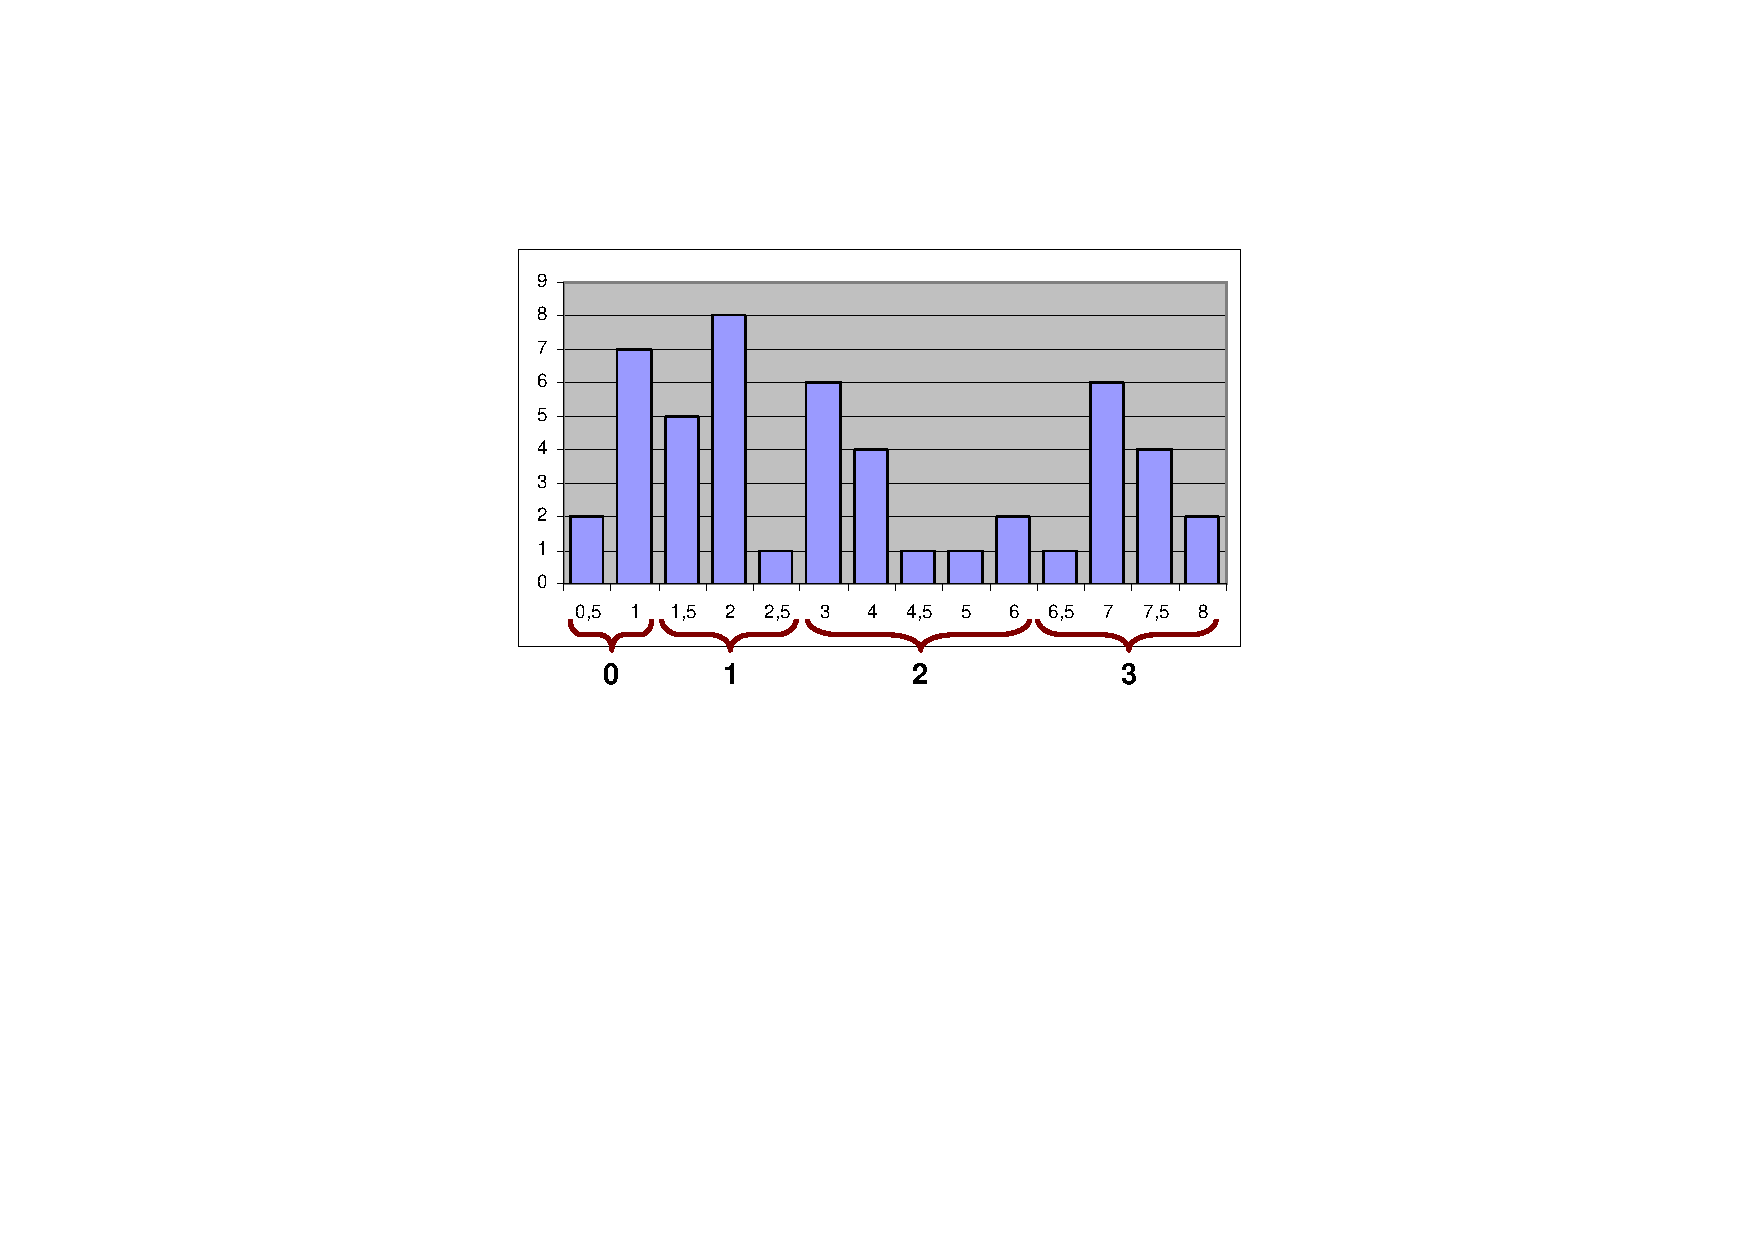
\includegraphics[angle=-90, width=0.6\hsize]{ranking_histogram}}
\caption{Frequencies of the seriousness ranking.}
\label{fig:data_ranking_histogram}
\end{figure}

Values of the overall seriousness ranking attribute were stated from ``a general impression'' made by the texts with respect to particular attributes. %(Figure~\ref{fig:attributes_description}). 
The values have evolved to 14 distinct values in the range from 0.5 to 8. 
A histogram with frequencies of all these values is in Figure~\ref{fig:data_ranking_histogram}.
We divided the values into four approximately equipotent groups 
(see in Figure~\ref{fig:data_ranking_histogram}) 
and these groups determine the target class attribute of the classification task. 
%and logic rules were learned for each group separately\footnote{We do not have a binary rule, which would return an exact value of the rating, but we have one ``true/false'' rule for each of the four categories.}.






\subsection{Classification Datasets from UCI ML Repository} \label{sec:data_uci_datasets}

UCI Machine Learning Repository\footnote{\url{http://archive.ics.uci.edu/ml/index.html}} \citep{biblio:UCI} is a large archive of machine learning datasets collected at the University of California, Irvine. Several classification datasets were selected and used in the evaluation of the Fuzzy ILP Classifier, see in Section~\ref{sec:fuzzy_eval_uci}.
The list of selected datasets can be found in Table~\ref{tab:UCI_datasets}. All the datasets are monotonizable (the target attribute can be naturally ordered), so the fuzzy classifier could take advantage of that.


\begin{table}
	\centering
	\begin{threeparttable}
		\begin{tabular}{lll}
shortcut & name & url suffix\tnote{a}\\
\hline
car    & Car Evaluation  & \href{http://archive.ics.uci.edu/ml/datasets/Car+Evaluation}{\ttfamily Car+Evaluation}\\
wine\tnote{b} & Wine Quality  & \href{http://archive.ics.uci.edu/ml/datasets/Wine+Quality}{\ttfamily Wine+Quality}\\
cmc    & Contraceptive Method Choice  & \href{http://archive.ics.uci.edu/ml/datasets/Contraceptive+Method+Choice}{\ttfamily Contraceptive+Method+Choice}\\
tae    & Teaching Assistant Evaluation  & \href{http://archive.ics.uci.edu/ml/datasets/Teaching+Assistant+Evaluation}{\ttfamily Teaching+Assistant+Evaluation}\\
pop    & Post-Operative Patient  & \href{http://archive.ics.uci.edu/ml/datasets/Post-Operative+Patient}{\ttfamily Post-Operative+Patient}\\
nurs   & Nursery  & \href{http://archive.ics.uci.edu/ml/datasets/Nursery}{\ttfamily Nursery}\\
\hline
		\end{tabular}
		\begin{tablenotes}
			\item [a] The prefix is: \url{http://archive.ics.uci.edu/ml/datasets/}
			\item [b] Only red wine part of the dataset was used.
		\end{tablenotes}
		\caption{Classification datasets selected form the UCI ML Repository.} \label{tab:UCI_datasets}
	\end{threeparttable}
	
\end{table}




\chapter{Experiments and Evaluation} \label{sec:ch_eval}

Experiments that were performed to evaluate our methods and approaches will be presented in this chapter. Four main sections separate the experiments by topic, to which they belong.

\section{Evaluation of Manual Rules} \graphicspath{{../img/ch50/}}


In this section, two experiments will be presented to explain the usefulness of our extraction method based on manually designed rules. 
The first one provides measurements on a higher amount of texts without manual gold standard annotations, while the second experiment was done on a small manually annotated collection. 

\subsection{Czech Fireman Quantitative} \label{sec:manual_quant_experiment}

We evaluated three extraction rules (one procedural and two Netgraph based) on a set of 814 texts of news of several Czech fire departments and measured several statics. All the rules had the same goal: to find numbers of people that died or were injured during an accident. The procedural rule was the same as in Figure~\ref{fig:btred_rule} and the Netgraph based rules correspond with the rule in Figure~\ref{fig:manual_extract_patern}. The only difference between the Netgraph rules is that in the first case (Netgraph 1) all rule nodes except number 1 (\verb+action_type+) were set as optional, while in the second case (Netgraph 2) also node 4 (participant) was compulsory. This little change caused some interesting effects -- see below. 

Table~\ref{tab:manual_tab_manual_rules} summarizes some of the statics that were measured. Description of individual values follows.

\begin{table}
	\centering
		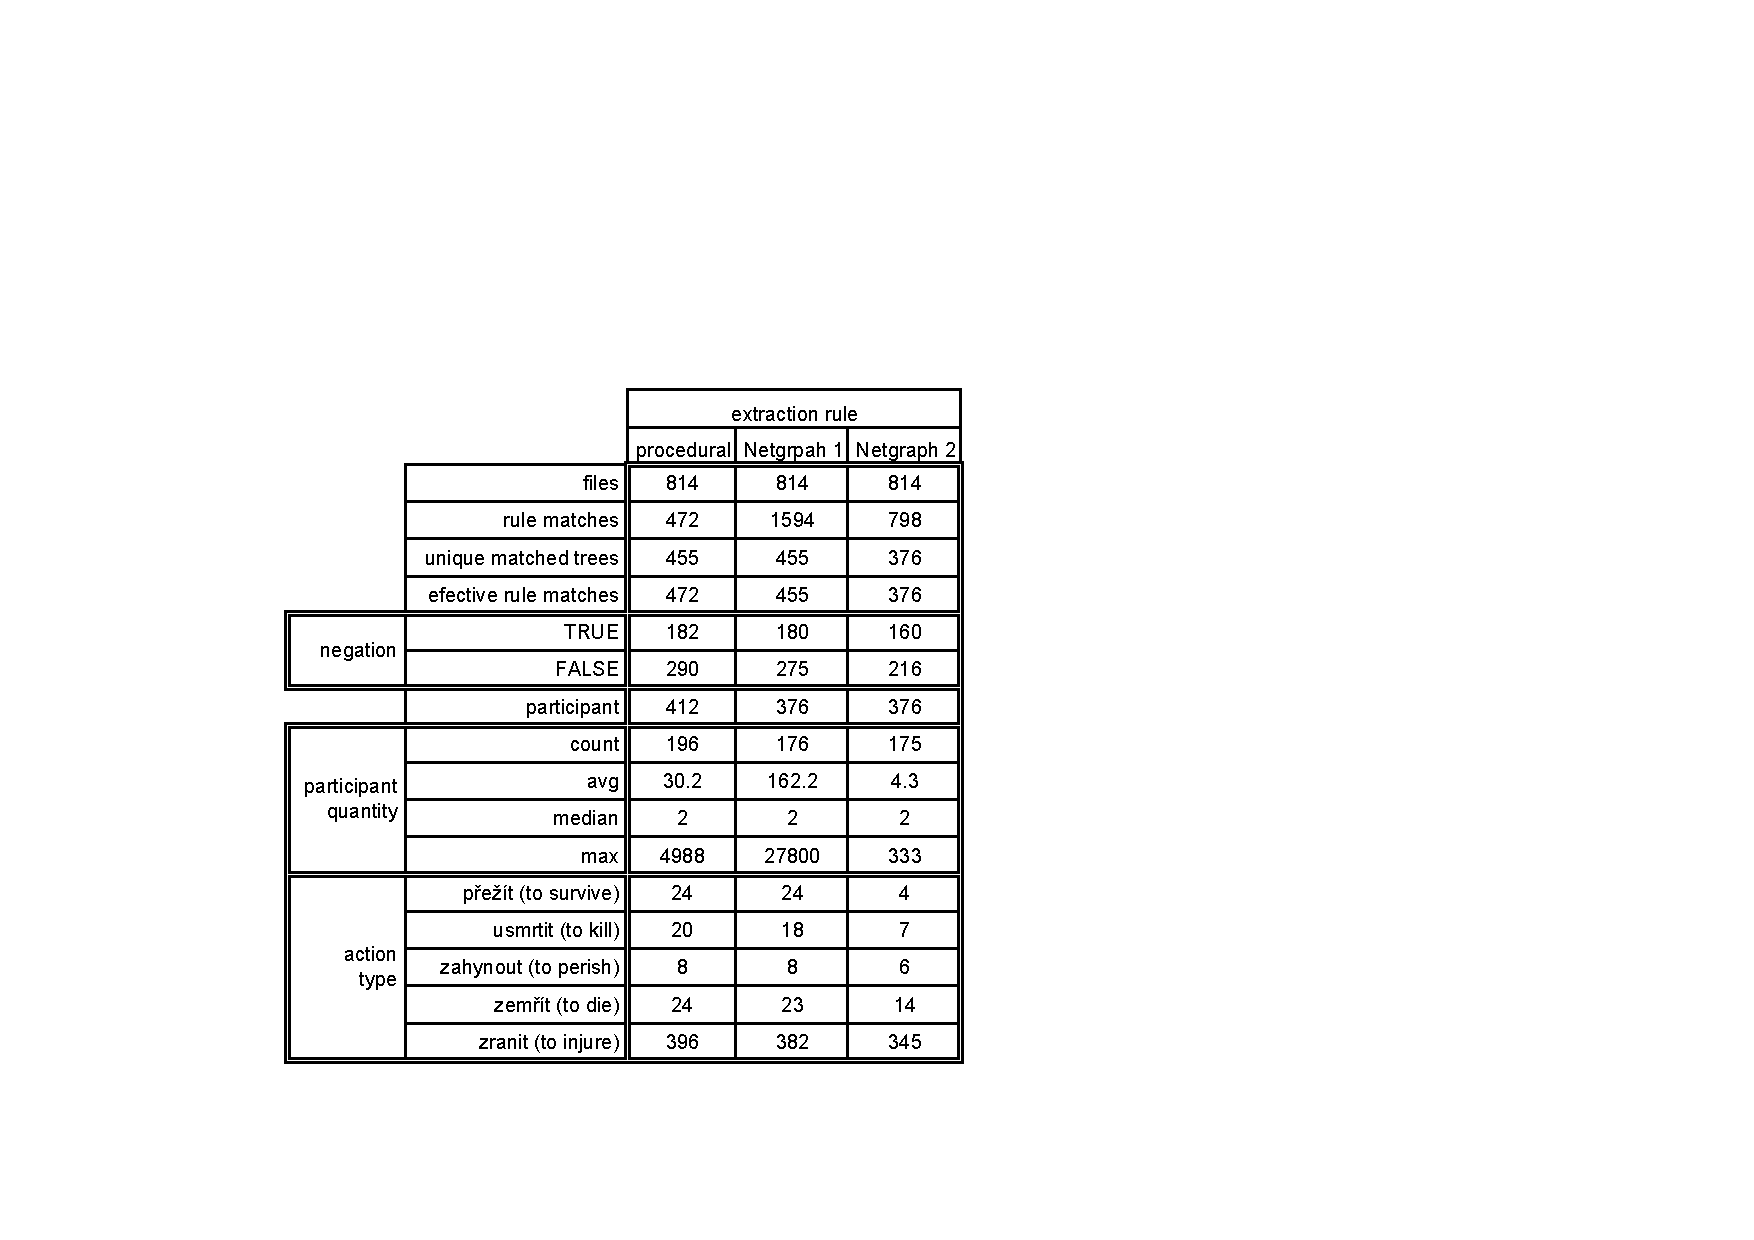
\includegraphics[angle=-90,width=0.6\hsize]{tab_manual_rules}
	\caption{Evaluation of manually created rules (bigger dataset without manual annotations).}
	\label{tab:manual_tab_manual_rules}
\end{table}


\begin{description}
	\item[Files]
The same set of 814 files (texts) was used in all the experiments.

	\item[Rule matches]
The presence of optional nodes in a query increases the number of possibilities how a Netgraph query can be matched to a single linguistic tree. An optional node might or might not be marked in the result. The number of possible matches is also increased if there are more compatible nodes in a candidate tree that can be matched with a single query node. This can even be true for the participant query node (4) in the case of Netgraph based rules if a sentence mentions more than one affected person. This can be marked as a mistake in the rule design -- it does not count with such possibility, or it can be taken as a drawback of the current evaluation algorithm of the Netgraph based method -- it should put all the possibilities to the output. Note that this issue does not concern the procedural method, which outputs all the matching participants.

	\item[Unique matched trees]
This number represents the number of unique trees matched by the extraction rule.

	\item[Effective rule matches]
Because the procedural rules and the Netgraph based rules are evaluated in a different way, the way of selection of effective matches (matches that are used for the output) is also different. In the procedural case all matches are used because every such match is tied up with a different verb in a sentence. In this case more matches per sentence (tree) are only possible for complex sentences with more verbs and therefore every match is applicable because it is connected with a different piece of information.\\
In the Netgraph case it is necessary to select the most relevant matches of all possible ones. The first longest (maximum of optional nodes) match for each tree is selected. This is unfortunately not optimal and also not consistent with the procedural case, but it is the easiest option for the implementation (Netgraph can be directly used in that case.)

	\item[Negation, participant, participant quantity (count), action type]
These values represent numbers of matching nodes (or more precisely of pieces of extracted information) of the given type. For example values of participant are the numbers of all participants (node number 4 in the Netgraph based rule) identified by the extraction rule and values of \emph{přežít} (survive) are numbers of matching action type nodes with the value of \emph{přežít} (survive). Note that some postprocessing of the Netgraph based output was necessary to count TRUE and FLASE negation values.

	\item[Participant quantity]
Values in this group are all connected with the quantity kind of information. It expresses the quantity of participants involved in the corresponding incident action. This kind of information is numeric so some numerical calculations can be made (average value, median and maximum value). Again postprocessing of the Netgraph based output was necessary to obtain these values -- in this case translation of seven kinds of numerals to numbers (\emph{jeden} - 1, \emph{dva} - 2, \emph{tři} - 3, \emph{čtyři} - 4, \emph{šest} - 6, \emph{sedm} - 7, \emph{osm} - 8). Note that the vale of average is strongly affected by the very few high numbers present in the results (the values 1 and 2 accounted for more than half of the results.)\\
Values of participant quantity also demonstrate several errors made by the particular extraction rules, see bellow for details.
\end{description}





















\subsubsection{Detected errors}

Results of the extraction were investigated only partly; no formal evaluation is available in this case (except on a small evaluation set, see bellow: the second experiment). About 10-20\% of information was not extracted because of errors of linguistic parsing; majority of the errors was made in long complex sentences, which are known to be difficult for linguistic processing. There was only a few of false positives. A nice example can be traced from the maximum values of participant quantity in Table~\ref{tab:manual_tab_manual_rules}. Three different numbers were found in the three experiments: 27800, 4988 and 333. The number of 27800 is actually a number of chickens that died during one of the accidents. The number was extracted by the first Netgraph based rule because the query node 4 (participant) was marked as optional and omitted during the evaluation. This node normally ensures that the participant is one of: person, man, woman, child, driver, etc.
Numbers 4988 and 333 are both correct. They were both used in the same sentence, which summarized numbers of injured (4988) and killed (333) people during one whole year. Although the sentence was quite complex it was linguistically parsed correctly and also the procedural rule managed to extract both numbers correctly. The Netgraph based rule extracted only the first number in the sentence because the current evaluation algorithm does not allow multiple matches per sentence (see above the comments of rule matches and effective rule matches).


\subsection{Czech Fireman Qualitative}


\begin{table}
	\centering
	\begin{tabular}{|r|c|c|c|c|c|c|}
		\hline
		 & correct & missing & spurious & recall & precision & $F_1$\\
		\hline
		injuries & 3 & 29 & 0 & 0.09 & 1 & 0.17\\
		\hline
		fatalities & 1 & 10 & 0 & 0.09 & 1 & 0.17\\
		\hline
	\end{tabular}
	\caption{Evaluation of the manually created rule form Figure~\ref{fig:manual_extract_patern} on the manually annotated dataset.}
	\label{tab:manual_extract_patern_eval}
\end{table}



In the second experiment a manually annotated collection of 50 fireman news texts was used. Having the extraction rule from the previous experiment and a set of manually annotated texts it is only natural to ask a question about the success of the extraction rule on that collection. Table~\ref{tab:manual_extract_patern_eval} summarizes the results. These results are far from satisfactory; the recall of 0.09 is something that is far from any acceptable use. Several explanations of the issue can be provided. The extraction rule serves more for a demonstration than for exhausting coverage of all possible cases. The extraction rule looks for particular verb (to injure, to die, etc.) but the information can be also expressed by an adjective (injured driver, death passenger, etc.); another extraction rules should be constructed for these and other cases. The training collection used for the design was also of a different spectrum of texts.



On the other hand this experiment shows how a manually annotated collection contributes to the quality of extraction rules. We can never know if the extraction rule is usable until a formal evaluated is made. Also the fact that the precision is strictly 1 should be noted. This means that the extraction rule made no mistake in those cases when it provided some output.



\subsubsection{Manual Design of Rules Using Training Data Set}  

\begin{table}
	\centering
	\begin{tabular}{|r|c|c|c|c|c|c|}
		\hline
		 & correct & missing & spurious & recall & precision & $F_1$\\
		\hline
		manual rules & 5 & 2 & 0 & 0.71 & 1 & 0.83\\
		\hline
		ILP rules & 5 & 2 & 0 & 0.71 & 1 & 0.83\\
		\hline
	\end{tabular}
	\caption{Evaluation of the manually created rules and ILP learned rules (manually annotated dataset was used for rule design (training half) and evaluation (testing half) -- see the description of the second experiment in text.)}
	\label{tab:manual_damage_manual_eval}
\end{table}

\begin{table}
	\centering
	\begin{tabular}{|r|c|c|c|c|c|c|}
		\hline
		 & correct & missing & spurious & recall & precision & $F_1$\\
		\hline
		manual rules & 4 & 1 & 1 & 0.8 & 0.8 & 0.8\\
		\hline
		ILP rules & 4 & 1 & 1 & 0.8 & 0.8 & 0.8\\
		\hline
	\end{tabular}
	\caption{Cross method comparison of found instances.}
	\label{tab:manual_damage_cross_method}
\end{table}




Next question that naturally emerges is: How would be the performance if the rules were designed with the support of a manually annotated collection? An additional experiment was made to answer that question. The collection was split into two even parts -- training part and testing part. A manually created rule was designed so that it correctly matched with all annotations of the training part and then it was evaluated on the testing part. For the validity of the experiment it was necessary that the designer did not have any knowledge about the data of the testing part; that is why we used a different extraction task (damage instead of injuries and fatalities). We have also compared the performance of the manually created rule with a rule learned by the ILP machine learning engine.

The results are summarized in Table~\ref{tab:manual_damage_manual_eval}. Both kinds of rules (manually designed and learned by ILP) performed the same (recall: 0.71, precision: 1); both the methods correctly found 5 instances and they were both unable to find 2 instances. From the cross coverage comparison in 
Table~\ref{tab:manual_damage_cross_method} it is apparent that the methods agreed on 4 instances and each method was able to discovered one instance that the other did not discover. Such results could be accepted for a practical application but we must not forget the fact that the collection is very small and only single evidence is provided by the experiment, so it dies not provide any statistical significance (getting statistically significant results would require experiments with different datasets, extraction tasks and human designers.) 

%\clearpage

\section{Evaluation of Learned Rules} \label{sec:learning_eval}

In this section, we present two experiments with two manually annotated datasets. The performance of our method based on ILP machine learning was measured and compared with an alternative extraction method based on propositional machine learning.

Evaluation of machine learning approaches is easier than evaluation of approaches based on manual extraction rules because it is not necessary to construct extraction rules for each experiment manually. Thanks to this fact and the availability of manually annotated datasets, the evaluation is more comprehensive than in the previous section.

\subsection{Examples of Learned Rules}

\begin{figure}
\begin{minted}[linenos,  fontsize=\footnotesize,
               frame=lines]{prolog}
% [cars - Rule 3] [Pos cover = 5 Neg cover = 0]
mention(cars,A) :-
   'lex.rf'(B,A), sempos(B,'n.denot'), tDependency(C,B), t_lemma(C,vozidlo), 
   functor(C,'ACT'), number(C,sg).   % vozidlo ~ vehicle

% [damage - Rule 1] [Pos cover = 14 Neg cover = 0]
mention(damage,A) :-
   'lex.rf'(B,A), sempos(B,'n.quant.def'), tDependency(C,B), tDependency(C,D), 
   t_lemma(D,'vyšetřovatel').   % vyšetřovatel ~ investigating officer

% [end_subtree - Rule 7] [Pos cover = 6 Neg cover = 0]
mention(end_subtree,A) :-
   'lex.rf'(B,A), sempos(B,'n.quant.def'), tDependency(C,B), t_lemma(C,'ukončit').
	    % ukončit ~ finish

% [start - Rule 2] [Pos cover = 15 Neg cover = 0]
mention(start,A) :-
   'lex.rf'(B,A), functor(B,'TWHEN'), tDependency(C,B), tDependency(C,D), 
   t_lemma(D,ohlásit).   % ohlásit ~ report (e.g. a fire)

% [injuries - Rule 1] [Pos cover = 7 Neg cover = 0]
mention(injuries,A) :-
   'lex.rf'(B,A), functor(B,'PAT'), tDependency(B,C), t_lemma(C,'zraněný'), 
   tDependency(D,B), aspect(D,cpl).   % zraněný ~ injured

% [fatalities - Rule 1] [Pos cover = 3 Neg cover = 0]
mention(fatalities,A) :-
   'lex.rf'(B,A), functor(B,'PAT'), tDependency(C,B), t_lemma(C,srazit).
	    % srazit ~ knock down

% [profesional_unit - Rule 1] [Pos cover = 17 Neg cover = 0]
mention(profesional_unit,A) :-
   'lex.rf'(B,A), functor(B,'LOC'), gender(B,fem), tDependency(C,B), 
   functor(C,'CONJ'), overlap_Lookup_tToken(D,B).

% [amateur_unit - Rule 1] [Pos cover = 19 Neg cover = 0]
mention(amateur_unit,A) :-
   'lex.rf'(B,A), tDependency(C,B), tDependency(D,C), tDependency(D,E), 
   t_lemma(E,dobrovolný).   % dobrovolný ~ voluntary
\end{minted}
	\caption{Rules with largest coverage for each task learned from the whole dataset \sectiondoubleref{sec:data_fireman_annotated}.}
	\label{fig:learning_eval_rules}
\end{figure}

In Figure~\ref{fig:learning_eval_rules}, we present the most representative examples of extraction rules learned from the whole dataset \sectiondoubleref{sec:data_fireman_annotated}. The rule with largest coverage for each extraction task was selected and it is provided in the figure. Each rule demonstrates a connection of the target token, annotated as `\emph{mention(task\_name)}’, with other parts of the sentence through linguistic syntax structures. 

For example the second rule (\emph{damage} task, lines 6-9) connects the node A with its tectogrammatical counterpart -- numeral B (\emph{n.quant.def}) and with node D (`vyšetřovatel') representing the investigating officer who stated the mount of damage. 



\subsection{Evaluation Methods and Measures}

Evaluation experiments have to be preformed repeatedly in order to investigate statistical significance. A dataset consisting of individual documents is randomly split into the training and testing part in each experimental run. The ratio between the training and testing part depends on the size of the dataset. It is important to have enough training data and therefore larger training part and smaller testing part is used if the dataset is too small. The cross validation technique meets exactly this requirement: the more cross validation folds, the greater the ratio. In following sections presenting individual experiments, different numbers of cross validation folds are used according to the sizes of the datasets.

In each experiment run, the performance is evaluated using several performance measures; precision, recall and $F_1$ (harmonic mean of precision and recall) are mostly used for information extraction experiments. Partially correct (or overlapping) matches can occur when annotations do not match exactly (they are overlapping). Strict, lenient and average variants of performance measures allow dealing with partially correct matches in different ways:
\begin{itemize}
	\item     Strict measures considers all partially correct matches as incorrect (spurious).
	\item     Lenient measures considers all partially correct matches as correct.
	\item     Average measures takes the average of strict and lenient.
\end{itemize}

See also the GATE documentation chapter about performance evaluation\footurl{http://gate.ac.uk/userguide/chap:eval}
and few details about the statistical significance in Section~\ref{sec:conclusion_statsig}.



\subsection{Comparison with PAUM Classifier}
To compare our solution with other alternatives, we took the PAUM (Perceptron Algorithm with Uneven Margins) propositional learner from GATE \citep{Li:Paum}. The quality of propositional learning from texts is strongly dependent on the selection of right features. We obtained quite good results with features of a window of two preceding and two following token lemmas and morphological tags. The precision was further improved by adding the feature of \emph{analytical function}\footurl{http://ufal.mff.cuni.cz/pdt2.0/doc/manuals/en/a-layer/html/ch03.html\#s1-list-anal-func} from the syntactic parser and information about presence of named entities.


%\subsection{Cross validation}
%We used the 10-fold cross validation in the evaluation. Thanks to this technique the evaluation is simple. After processing all the folds each document is processed with some of the ten learned models such that the particular document was not used in learning of that model, so all documents are unseen by the model applied on them. At the end we just compare the gold standard annotations with the learned ones in all documents.


\subsection{Czech Fireman Performance}

Table~\ref{tab:learning_eval_fir_perfom} summarizes performance evaluation of our ILP based method and its comparison with PAUM classifier on the dataset \sectiondoubleref{sec:data_fireman_annotated}. The table shows results of the three main evaluation measures: strict precision, strict recall and strict $F_1$ for each extraction task as well as overall results. 8-fold cross validation was performed 8 times in the experiment. Average values and standard deviations are printed in the table and statistical significance is indicated. Root/subtree preprocessing/postprocessing (Section~\ref{sec:learning_root_subtree}) was performed in the first three tasks: `cars’, `damage’ and `end subtree’.

Although the precision of the ILP method was better in the majority of tasks and also its overall precision is statically better than the precision of the PAUM method, its recall was worse in all the measurements and also $F_1$ score is indicating better results of the PAUM method. 


\begin{table}[ht!]
\centering 
\begin{tabular}
{lcrclcrcl@{\hspace{0.1cm}}cc}

\multicolumn{11}{c}{Strict Precision}\\
\hline
Task && \multicolumn{3}{c}{ILP}  && \multicolumn{3}{c}{PAUM} && \\
\hline
              cars &&      0.324 &  $\pm$  &       0.387 & &      0.380 &  $\pm$  &       0.249 &  \\
            damage &&      0.901 &  $\pm$  &       0.178 & &      0.860 &  $\pm$  &       0.176 &  \\
       end subtree &&      0.529 &  $\pm$  &       0.381 & &      0.499 &  $\pm$  &       0.242 &  \\
             start &&      0.929 &  $\pm$  &       0.109 & &      0.651 &  $\pm$  &       0.152 & $\bullet$ \\
          injuries &&      0.667 &  $\pm$  &       0.291 & &      0.398 &  $\pm$  &       0.205 & $\bullet$ \\
        fatalities &&      0.814 &  $\pm$  &       0.379 & &      0.307 &  $\pm$  &       0.390 & $\bullet$ \\
  profesional unit &&      0.500 &  $\pm$  &       0.241 & &      0.677 &  $\pm$  &       0.138 & $\circ$ \\
      amateur unit &&      0.863 &  $\pm$  &       0.256 & &      0.546 &  $\pm$  &       0.293 & $\bullet$ \\
\hline
           overall &&      0.691 &  $\pm$  &       0.358 & &      0.540 &  $\pm$  &       0.297 & $\bullet$ \\
\hline
\\

\multicolumn{11}{c}{Strict Recall}\\
\hline
Task && \multicolumn{3}{c}{ILP}  && \multicolumn{3}{c}{PAUM} && \\
\hline
              cars &&      0.088 &  $\pm$  &       0.129 & &      0.353 &  $\pm$  &       0.231 & $\circ$ \\
            damage &&      0.821 &  $\pm$  &       0.261 & &      0.933 &  $\pm$  &       0.148 & $\circ$ \\
       end subtree &&      0.231 &  $\pm$  &       0.203 & &      0.601 &  $\pm$  &       0.249 & $\circ$ \\
             start &&      0.908 &  $\pm$  &       0.115 & &      0.978 &  $\pm$  &       0.058 & $\circ$ \\
          injuries &&      0.574 &  $\pm$  &       0.309 & &      0.814 &  $\pm$  &       0.224 & $\circ$ \\
        fatalities &&      0.388 &  $\pm$  &       0.449 & &      0.536 &  $\pm$  &       0.452 & $\circ$ \\
  profesional unit &&      0.506 &  $\pm$  &       0.191 & &      0.811 &  $\pm$  &       0.138 & $\circ$ \\
      amateur unit &&      0.886 &  $\pm$  &       0.210 & &      0.955 &  $\pm$  &       0.096 & $\circ$ \\
\hline
           overall &&      0.550 &  $\pm$  &       0.382 & &      0.748 &  $\pm$  &       0.312 & $\circ$ \\
\hline
\\

\multicolumn{11}{c}{Strict $F_1$}\\
\hline
Task && \multicolumn{3}{c}{ILP}  && \multicolumn{3}{c}{PAUM} && \\
\hline
              cars &&      0.109 &  $\pm$  &       0.147 & &      0.335 &  $\pm$  &       0.205 & $\circ$ \\
            damage &&      0.828 &  $\pm$  &       0.217 & &      0.876 &  $\pm$  &       0.131 & $\circ$ \\
       end subtree &&      0.283 &  $\pm$  &       0.219 & &      0.525 &  $\pm$  &       0.213 & $\circ$ \\
             start &&      0.912 &  $\pm$  &       0.089 & &      0.771 &  $\pm$  &       0.111 & $\bullet$ \\
          injuries &&      0.543 &  $\pm$  &       0.280 & &      0.498 &  $\pm$  &       0.204 &  \\
        fatalities &&      0.306 &  $\pm$  &       0.420 & &      0.222 &  $\pm$  &       0.308 &  \\
  profesional unit &&      0.491 &  $\pm$  &       0.200 & &      0.730 &  $\pm$  &       0.118 & $\circ$ \\
      amateur unit &&      0.827 &  $\pm$  &       0.253 & &      0.634 &  $\pm$  &       0.296 & $\bullet$ \\
\hline
           overall &&      0.537 &  $\pm$  &       0.369 & &      0.574 &  $\pm$  &       0.295 & $\circ$ \\
\hline
\\
\multicolumn{11}{c}{$\circ$, $\bullet$ statistically significant improvement or degradation}\\
\end{tabular}

\caption{Evaluation on Czech Fireman dataset} \label{tab:learning_eval_fir_perfom}
\end{table}




Table~\ref{tab:learning_eval_fir_time} provides learning and application (or testing) times of the compared methods. It is clear that learning time of the ILP method is many times higher than the time of the PAUM method. For example the `cars’ task took the ILP method approximately three and half minutes while the PAUM method spent only two seconds on it. On the other hand, the testing or application time of the ILP method is not that much higher than the time of the PAUM method 
%and once the extraction rules are done, the time requirements of the ILP method are acceptable.
but we have to notice that these times do not include linguistic preprocessing and deep language parsing needed by the ILP method will increase the time significantly.

Detailed results with much more evaluation measurements including lenient variants are available in the appendix -- Section~\ref{sec:complete_eval_fire}.

%\clearpage
%\subsection{Czech Fireman Time}


\begin{table}
\centering 
\begin{tabular}
{lcrclcrcl@{\hspace{0.1cm}}cc}

\multicolumn{11}{c}{Time Training}\\
\hline
Task && \multicolumn{3}{c}{ILP}  && \multicolumn{3}{c}{PAUM} && \\
\hline
              cars &&     3:28.0 &  $\pm$  &      0:28.3 & &     0:02.2 &  $\pm$  &      0:00.1 & $\bullet$ \\
            damage &&     0:23.4 &  $\pm$  &      0:06.2 & &     0:02.2 &  $\pm$  &      0:00.1 & $\bullet$ \\
       end subtree &&     1:34.2 &  $\pm$  &      0:14.4 & &     0:02.2 &  $\pm$  &      0:00.1 & $\bullet$ \\
             start &&     0:28.9 &  $\pm$  &      0:03.1 & &     0:02.2 &  $\pm$  &      0:00.1 & $\bullet$ \\
          injuries &&     1:30.7 &  $\pm$  &      0:15.0 & &     0:02.2 &  $\pm$  &      0:00.1 & $\bullet$ \\
        fatalities &&     0:49.2 &  $\pm$  &      0:10.6 & &     0:02.2 &  $\pm$  &      0:00.1 & $\bullet$ \\
  profesional unit &&     2:37.4 &  $\pm$  &      0:27.4 & &     0:02.2 &  $\pm$  &      0:00.1 & $\bullet$ \\
      amateur unit &&     0:24.0 &  $\pm$  &      0:04.6 & &     0:02.2 &  $\pm$  &      0:00.1 & $\bullet$ \\
\hline
           overall &&     1:24.5 &  $\pm$  &      1:05.8 & &     0:02.2 &  $\pm$  &      0:00.1 & $\bullet$ \\
\hline
\\

\multicolumn{11}{c}{Time Testing}\\
\hline
Task && \multicolumn{3}{c}{ILP}  && \multicolumn{3}{c}{PAUM} && \\
\hline
              cars &&     0:00.9 &  $\pm$  &      0:00.2 & &     0:00.3 &  $\pm$  &      0:00.1 & $\bullet$ \\
            damage &&     0:00.9 &  $\pm$  &      0:00.1 & &     0:00.3 &  $\pm$  &      0:00.0 & $\bullet$ \\
       end subtree &&     0:00.9 &  $\pm$  &      0:00.2 & &     0:00.3 &  $\pm$  &      0:00.0 & $\bullet$ \\
             start &&     0:00.9 &  $\pm$  &      0:00.1 & &     0:00.3 &  $\pm$  &      0:00.0 & $\bullet$ \\
          injuries &&     0:00.9 &  $\pm$  &      0:00.2 & &     0:00.3 &  $\pm$  &      0:00.1 & $\bullet$ \\
        fatalities &&     0:00.9 &  $\pm$  &      0:00.1 & &     0:00.3 &  $\pm$  &      0:00.0 & $\bullet$ \\
  profesional unit &&     0:00.9 &  $\pm$  &      0:00.1 & &     0:00.3 &  $\pm$  &      0:00.0 & $\bullet$ \\
      amateur unit &&     0:00.9 &  $\pm$  &      0:00.1 & &     0:00.3 &  $\pm$  &      0:00.0 & $\bullet$ \\
\hline
           overall &&     0:00.9 &  $\pm$  &      0:00.1 & &     0:00.3 &  $\pm$  &      0:00.0 & $\bullet$ \\
\hline
\\
\multicolumn{11}{c}{$\bullet$ statistically significant decrease (not improvement in this case)}\\
\end{tabular}

\medskip
The time in this table is cumulative (sum over all folds in one experiment run).

\caption{Time spent by ML engines on the Czech Fireman dataset.} \label{tab:learning_eval_fir_time}
\end{table}





%\clearpage

\subsection{Acquisitions Performance} \label{sec:learning_eval_acq}

\begin{table}[th!]
\centering 
\begin{tabular}
{lcrclcrcl@{\hspace{0.1cm}}cc}

\multicolumn{11}{c}{Strict Precision}\\
\hline
Task && \multicolumn{3}{c}{ILP}  && \multicolumn{3}{c}{PAUM} && \\
\hline
            acqabr &&      0.457 &  $\pm$  &       0.034 & &      0.408 &  $\pm$  &       0.015 & $\bullet$ \\
          acquired &&      0.376 &  $\pm$  &       0.028 & &      0.441 &  $\pm$  &       0.027 & $\circ$ \\
            dlramt &&      0.286 &  $\pm$  &       0.052 & &      0.597 &  $\pm$  &       0.030 & $\circ$ \\
          purchabr &&      0.318 &  $\pm$  &       0.050 & &      0.390 &  $\pm$  &       0.015 & $\circ$ \\
         purchaser &&      0.403 &  $\pm$  &       0.037 & &      0.474 &  $\pm$  &       0.029 & $\circ$ \\
            seller &&      0.261 &  $\pm$  &       0.071 & &      0.245 &  $\pm$  &       0.041 &  \\
         sellerabr &&      0.306 &  $\pm$  &       0.111 & &      0.219 &  $\pm$  &       0.036 & $\bullet$ \\
\hline
           overall &&      0.344 &  $\pm$  &       0.088 & &      0.396 &  $\pm$  &       0.125 & $\circ$ \\
\hline
\\

\multicolumn{11}{c}{Strict Recall}\\
\hline
Task && \multicolumn{3}{c}{ILP}  && \multicolumn{3}{c}{PAUM} && \\
\hline
            acqabr &&      0.180 &  $\pm$  &       0.025 & &      0.517 &  $\pm$  &       0.027 & $\circ$ \\
          acquired &&      0.272 &  $\pm$  &       0.054 & &      0.512 &  $\pm$  &       0.033 & $\circ$ \\
            dlramt &&      0.276 &  $\pm$  &       0.043 & &      0.740 &  $\pm$  &       0.063 & $\circ$ \\
          purchabr &&      0.120 &  $\pm$  &       0.041 & &      0.514 &  $\pm$  &       0.033 & $\circ$ \\
         purchaser &&      0.340 &  $\pm$  &       0.064 & &      0.556 &  $\pm$  &       0.028 & $\circ$ \\
            seller &&      0.131 &  $\pm$  &       0.047 & &      0.226 &  $\pm$  &       0.046 & $\circ$ \\
         sellerabr &&      0.050 &  $\pm$  &       0.027 & &      0.190 &  $\pm$  &       0.032 & $\circ$ \\
\hline
           overall &&      0.196 &  $\pm$  &       0.106 & &      0.465 &  $\pm$  &       0.184 & $\circ$ \\
\hline
\\

\multicolumn{11}{c}{Strict $F_1$}\\
\hline
Task && \multicolumn{3}{c}{ILP}  && \multicolumn{3}{c}{PAUM} && \\
\hline
            acqabr &&      0.258 &  $\pm$  &       0.030 & &      0.456 &  $\pm$  &       0.015 & $\circ$ \\
          acquired &&      0.313 &  $\pm$  &       0.046 & &      0.473 &  $\pm$  &       0.024 & $\circ$ \\
            dlramt &&      0.280 &  $\pm$  &       0.046 & &      0.659 &  $\pm$  &       0.022 & $\circ$ \\
          purchabr &&      0.172 &  $\pm$  &       0.050 & &      0.443 &  $\pm$  &       0.016 & $\circ$ \\
         purchaser &&      0.367 &  $\pm$  &       0.051 & &      0.511 &  $\pm$  &       0.022 & $\circ$ \\
            seller &&      0.170 &  $\pm$  &       0.050 & &      0.232 &  $\pm$  &       0.036 & $\circ$ \\
         sellerabr &&      0.085 &  $\pm$  &       0.044 & &      0.202 &  $\pm$  &       0.030 & $\circ$ \\
\hline
           overall &&      0.235 &  $\pm$  &       0.101 & &      0.425 &  $\pm$  &       0.150 & $\circ$ \\
\hline
\\
\multicolumn{11}{c}{$\circ$, $\bullet$ statistically significant improvement or degradation}\\
\end{tabular}

\caption{Evaluation on Acquisitions dataset} \label{tab:learning_acq_eval}
\end{table}




The second experiment made with our ILP based extraction method was performed on the dataset \sectiondoubleref{sec:data_corporate_acquisitions}. Table~\ref{tab:learning_acq_eval} provides the same measurements as in the previous experiment. This time, 2-fold cross validation was performed 10 times; root/subtree preprocessing/postprocessing was performed in the `dlramt’ task only and the technique of learning on named entity roots (see Section~\ref{sec:learning_ne_roots}) was used on the rest of the tasks.

On this dataset, the PAUM method performed significantly better than the ILP method. There are only three tasks (`acqabr’, `seller’ and `sellerabr’), where the ILP method achieved better precision than the PAUM method and only two of the measurements are statistically significant. 

\begin{table}[th!]
\centering 
\begin{tabular}
{lcrclcrcl@{\hspace{0.1cm}}cc}

\multicolumn{11}{c}{Time Training}\\
\hline
Task && \multicolumn{3}{c}{ILP}  && \multicolumn{3}{c}{PAUM} && \\
\hline
            acqabr &&    16:24.9 &  $\pm$  &      8:22.9 & &     0:10.0 &  $\pm$  &      0:00.6 & $\bullet$ \\
          acquired &&    10:16.0 &  $\pm$  &      7:11.1 & &     0:09.8 &  $\pm$  &      0:00.4 & $\bullet$ \\
            dlramt &&    23:27.6 &  $\pm$  &     15:45.7 & &     0:10.8 &  $\pm$  &      0:02.8 & $\bullet$ \\
          purchabr &&    16:51.6 &  $\pm$  &      9:14.7 & &     0:10.2 &  $\pm$  &      0:01.4 & $\bullet$ \\
         purchaser &&    12:27.1 &  $\pm$  &      7:22.6 & &     0:10.4 &  $\pm$  &      0:01.2 & $\bullet$ \\
            seller &&     9:12.2 &  $\pm$  &      3:55.2 & &     0:10.1 &  $\pm$  &      0:01.0 & $\bullet$ \\
         sellerabr &&     6:11.5 &  $\pm$  &      4:03.3 & &     0:09.7 &  $\pm$  &      0:00.3 & $\bullet$ \\
\hline
           overall &&    13:33.0 &  $\pm$  &     10:00.1 & &     0:10.1 &  $\pm$  &      0:01.3 & $\bullet$ \\
\hline
\\

\multicolumn{11}{c}{Time Testing}\\
\hline
Task && \multicolumn{3}{c}{ILP}  && \multicolumn{3}{c}{PAUM} && \\
\hline
            acqabr &&     0:27.4 &  $\pm$  &      0:00.8 & &     0:13.6 &  $\pm$  &      0:00.3 & $\bullet$ \\
          acquired &&     0:26.7 &  $\pm$  &      0:00.7 & &     0:11.8 &  $\pm$  &      0:00.3 & $\bullet$ \\
            dlramt &&     0:30.5 &  $\pm$  &      0:00.8 & &     0:09.8 &  $\pm$  &      0:00.5 & $\bullet$ \\
          purchabr &&     0:27.4 &  $\pm$  &      0:00.9 & &     0:13.2 &  $\pm$  &      0:00.5 & $\bullet$ \\
         purchaser &&     0:27.5 &  $\pm$  &      0:02.0 & &     0:11.5 &  $\pm$  &      0:01.2 & $\bullet$ \\
            seller &&     0:27.3 &  $\pm$  &      0:03.2 & &     0:10.7 &  $\pm$  &      0:00.8 & $\bullet$ \\
         sellerabr &&     0:26.1 &  $\pm$  &      0:00.7 & &     0:11.5 &  $\pm$  &      0:00.3 & $\bullet$ \\
\hline
           overall &&     0:27.6 &  $\pm$  &      0:02.0 & &     0:11.7 &  $\pm$  &      0:01.4 & $\bullet$ \\
\hline
\\
\multicolumn{11}{c}{$\bullet$ statistically significant decrease (not improvement in this case)}\\
\end{tabular}

\caption{Time spent by ML engines on the Acquisitions dataset.} \label{tab:learning_acq_time}
\end{table}

Table~\ref{tab:learning_acq_time} provides learning and application (or testing) times on this dataset. Again, learning times of the ILP method are several times higher than the times of the PAUM method and there is not so big difference between application times, although the same notice about the necessity of deep language parsing in the preprocessing step pays also in this case. 

An interesting observation can be made when comparing training times of the ILP method on tasks, where the technique of learning on named entity roots was performed, with the remaining task `dlramt’. Table~\ref{tab:data_acquisitions} presents numbers of annotations per extraction task and it can be seen that the training time quite correlate with the number of annotations. But the task `dlramt’ has almost the least instances form the tasks used in the evaluation and its average training time is about two times higher than the time spent on other tasks and from there it can be seen that the technique of  learning on named entity roots can save training time. 

Detailed results with much more evaluation measurements including lenient variants are available in the appendix -- Section~\ref{sec:complete_eval_acq}.


%\clearpage

%\subsection{Acquisitions Time}


%\clearpage

%%%%%%%%%%%%%%%%%%%%%%%%%%%%%%%%%%%%%%%%%%%%%%%%%%%%%%%%%%%%%%%%%%%%%%%%%%%%%%%%%%%%%%%%%%%%%%%%%%%%%%%%%%%%%%
%%%%%%%%%%%%%%%%%%%%%%%%%%%%%%%%%%%%%%%%%%%%%%%%%%%%%%%%%%%%%%%%%%%%%%%%%%%%%%%%%%%%%%%%%%%%%%%%%%%%%%%%%%%%%%
%%%%%%%%%%%%%%%%%%%%%%%%%%%%%%%%%%%%%%%%%%%%%%%%%%%%%%%%%%%%%%%%%%%%%%%%%%%%%%%%%%%%%%%%%%%%%%%%%%%%%%%%%%%%%%
\section{Evaluation of Shareable Extraction Ontologies}  \label{sec:onto_experiment}

In this section we present an experiment that should serve as a proof of a concept that the proposed idea of independent extraction ontologies is realizable. We have selected several reasoners (namely Jena, HermiT, Pellet and FaCT++) and tested them on two slightly different datasets from two different domains and languages (see Table~\ref{tab:datasets}). This should at least partially demonstrate the universality of the proposed approach.

In both cases the task is to find all instances (corresponding to words in a document) that should be uncovered by the extraction rules. The extraction rules are saved in single extraction ontology for each dataset. The datasets are divided into individual document ontologies (owl files) corresponding to the individual documents. During the experiment the individual document ontologies are processed separately (one ontology in a step) by a selected reasoner. The total time taken to process all document ontologies of a dataset is the measured result of the reasoner for the dataset.

The actual reasoning tasks are more difficult than a simple retrieval of all facts entailed by the extraction rules. Such simple retrieval task took only a few seconds for the Acquisitions v1.1 dataset (including parsing) in the native Prolog environment that the IE engine uses. There were several more inferences needed in the reasoning tasks because the schema of the input files was a little bit different from the schema used in rules. The mapping of the schemas was captured in another ``mapping'' ontology that was included in the reasoning. The mapping ontology is a part of the publically available project ontologies.
%\footnote{See ``Data/ontologies'' link on the project page \url{http://czsem.berlios.de/}}%and a potentially interested reader can find the complete mapping ontology on the project's web site.


\subsection{Datasets} \label{sec:onto_datasets}

In the experiment we used two slightly different datasets from two different domains and languages.  Table~\ref{tab:datasets} summarizes some basic information about them. The fist dataset is called `czech\_fireman', it is based on Czech texts that are reporting on fire and traffic accidents and it was already described in Section~\ref{sec:data_rdf_fireman}. The second dataset is called ``Corporate Acquisition Events'', it is based on news articles describing acquisition events, taken from the Reuters dataset and it was already described in Section~\ref{sec:data_rdf_acquisitions}.

\begin{table}
\begin{center}
\begin{tabular}{|r||l|l|b{20mm}|b{20mm}|b{20mm}|}
%\begin{tabular}{|r||r|r|c|r|c|}
\hline
dataset & domain & language & number of~files &  dataset size (MB) &  number of~rules  \\
\hline
\hline
\textbf{czech\_fireman} & accidents & Czech &  50 &  16 &  2\\
\hline
\textbf{acquisitions} & finance & English &  600 &  126 &  113\\
\hline
\end{tabular}
\caption{Description of datasets that were used.}\label{tab:datasets}
\end{center}
\end{table}




\subsection{Reasoners}

%In the experiment we used four OWL reasoners
Four OWL reasoners were used in the experiment(namely
Jena\footnote{\url{http://jena.sourceforge.net}}
,HermiT\footnote{\url{http://hermit-reasoner.com}}
,Pellet\footnote{\url{http://clarkparsia.com/pellet}}
and FaCT++\footnote{\url{http://code.google.com/p/factplusplus}}
) and the time they spent on processing a particular dataset was measured. The time also includes time spent on parsing the input. HermiT, Pellet and FaCT++ were called through OWL API-3.1, so the same parser was used for them. Jena reasoner was used in its native environment with the Jena parser.
In the early beginning of the experiment we had to exclude the FaCT++ reasoner from both tests. It turned out that FaCT++ does not work with rules\footnote{\url{http://en.wikipedia.org/wiki/Semantic_reasoner#Reasoner_comparison}} and it did not return any result instances.  All the remaining reasoners strictly agreed on the results and returned the same sets of instances.

Also HermiT was not fully evaluated on the Acquisitions v1.1 dataset because it was too slow. The reasoner spent 13 hours of running to process only 30 of 600 files of the dataset. And it did not seem useful to let it continue. We contacted the authors of HermiT to clarify this issue and we were reminded that HermiT was mainly designed as a TBox reasoner and it was particularly optimized for the ontology classification problem \citep{ghms10classification}; it was never optimized for simple rule based (ABox) inferences.












\subsection{Evaluation Results}



\begin{table}
\begin{center}
\begin{tabular}{|r||r|r||r|r|}
\hline
reasoner & \textbf{czech\_fireman} & stdev & \textbf{acquisitions-v1.1} & stdev\\
\hline
\hline
\textbf{Jena} & 161 s & 0.226 & 1259 s & 3.579\\
\hline
\textbf{HermiT} & 219 s & 1.636 & $\gg$ 13 hours & \\
\hline
\textbf{Pellet} & 11 s & 0.062 & 503 s & 4.145\\
\hline
\textbf{FaCT++} & \multicolumn{4}{|c|}{Does not support rules.}\\
\hline
\end{tabular}
\end{center}

Time is measured in seconds. Average values from 6 measurements. Experiment environment: Intel Core I7-920 CPU 2.67GHz, 3GB of RAM, Java SE 1.6.0\_03, Windows XP.

\caption{Time performance of tested reasoners on both datasets.}
\label{tab:results}
\end{table}

Table~\ref{tab:results} summarizes results of the experiment. The standard deviations are relatively small when compared to the differences between the average times.  So there is no doubt about the order of the tested reasoners. Pellet performed the best and HermiT was the slowest amongst the tested and usable reasoners in this experiment.

From the results we can conclude that similar tasks can be satisfactorily solved by contemporary OWL reasoners because three of four tested reasoners were working correctly and two reasoners finished in bearable time.

On the other hand even the fastest system took 8.5 minutes to process 113 rules over 126MB of data. This is clearly   significantly longer than a operational system would require. 
Contemporary Semantic Web reasoners are known still to be often quite inefficient and the experiment showed that using them today to do information extraction will result in quite poor performance. However, efficiency problems can be solved
and in the context of Linked Data providing shareable descriptions of information extraction rules may be valuable.















%%%%%%%%%%%%%%%%%%%%%%%%%%%%%%%%%%%%%%%%%%%%%%%%%%%%%%%%%%%%%%%%%%%%%%%%%%%%%%%%%%%%%%%%%%%%%%%%%%%%%%%%%%%%%%
%%%%%%%%%%%%%%%%%%%%%%%%%%%%%%%%%%%%%%%%%%%%%%%%%%%%%%%%%%%%%%%%%%%%%%%%%%%%%%%%%%%%%%%%%%%%%%%%%%%%%%%%%%%%%%
%%%%%%%%%%%%%%%%%%%%%%%%%%%%%%%%%%%%%%%%%%%%%%%%%%%%%%%%%%%%%%%%%%%%%%%%%%%%%%%%%%%%%%%%%%%%%%%%%%%%%%%%%%%%%%
\section{Evaluation of Fuzzy ILP Classification} \label{sec:fuzzy_eval}
\graphicspath{{../img/ch80/}}

\begin{figure}[p]
\centerline{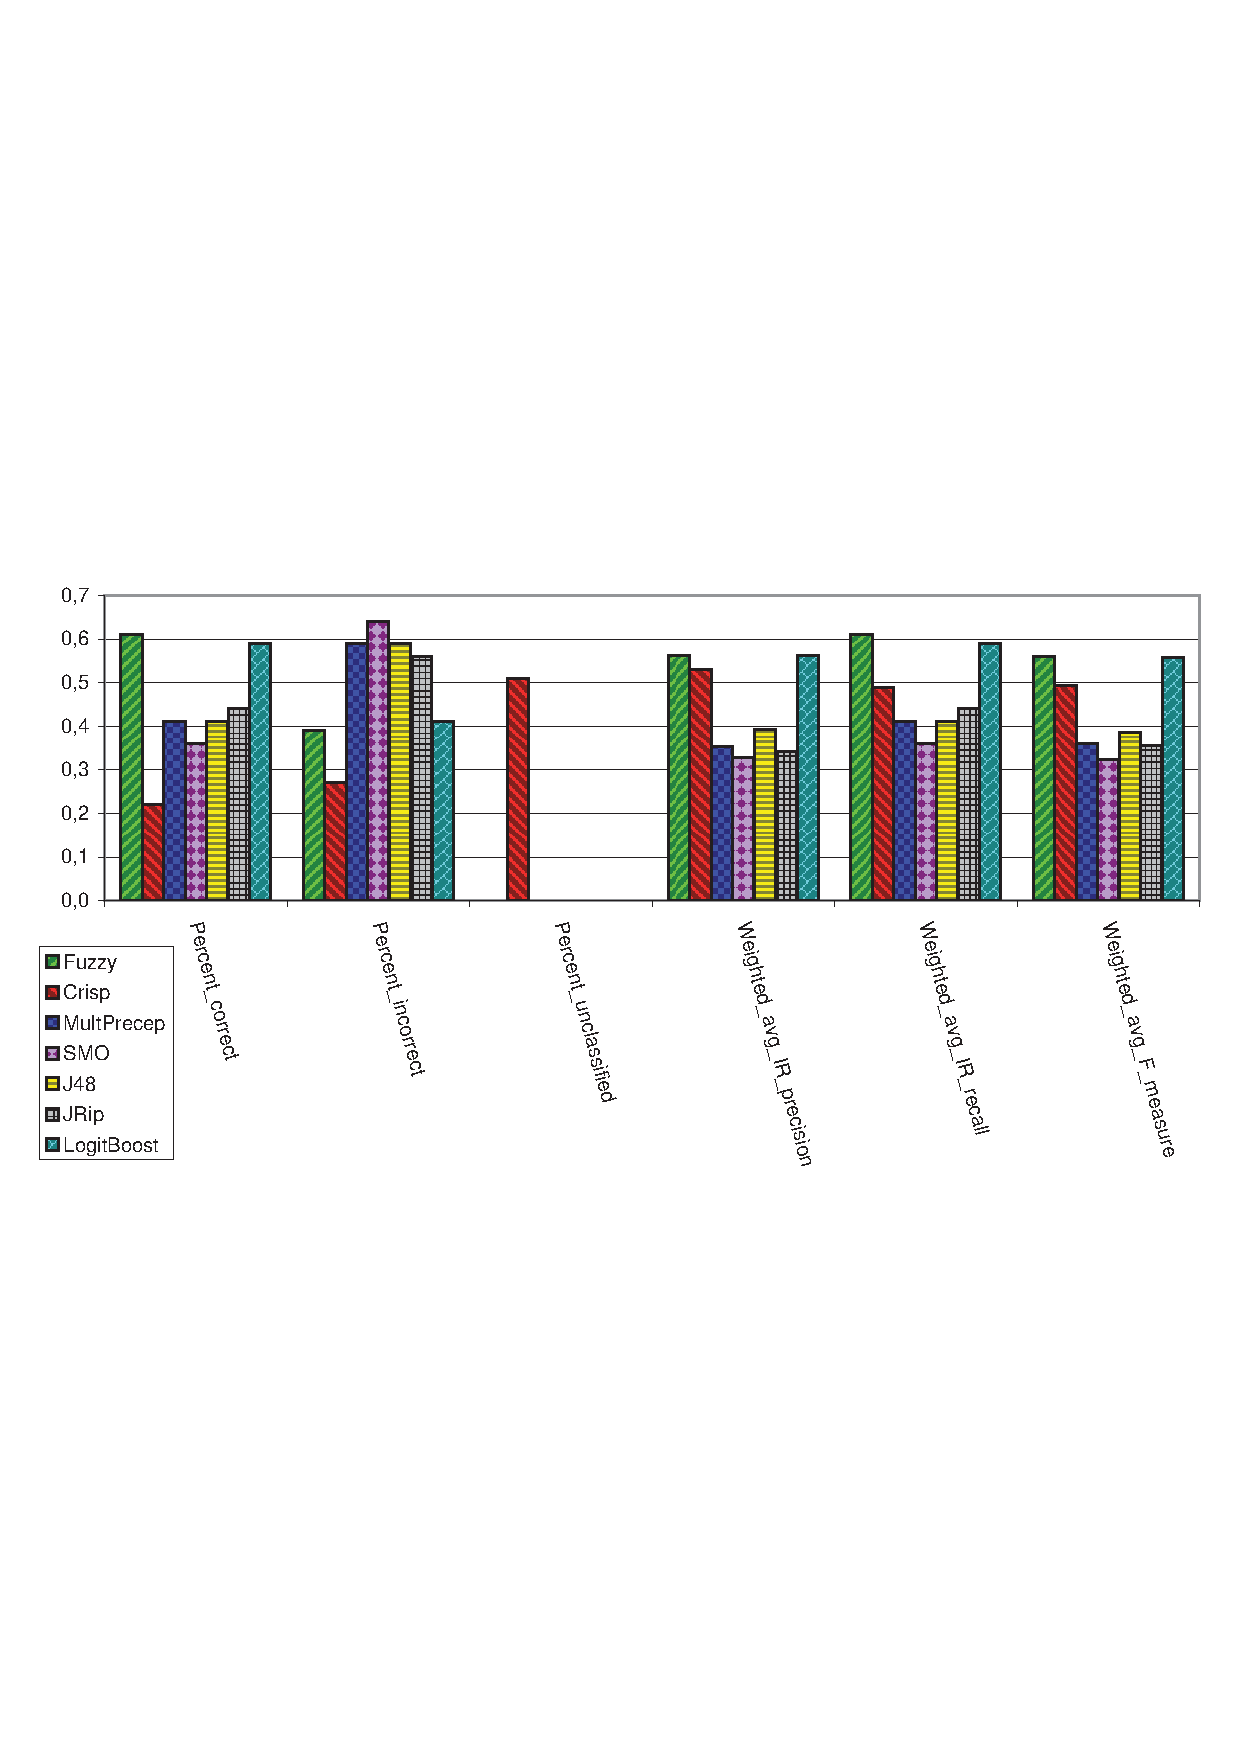
\includegraphics[width=0.8\hsize]{2x10cross}}
\caption{Evaluation of the methods -- average values.}
\label{fig:graph2x10}
\end{figure}


\begin{table}[p]
\scriptsize
{\centering \begin{tabular}{lr@{\hspace{0cm}}c@{\hspace{0cm}}rr@{\hspace{0cm}}c@{\hspace{0cm}}r@{\hspace{0.05cm}}cr@{\hspace{0cm}}c@{\hspace{0cm}}r@{\hspace{0.05cm}}cr@{\hspace{0cm}}c@{\hspace{0cm}}r@{\hspace{0.05cm}}cr@{\hspace{0cm}}c@{\hspace{0cm}}r@{\hspace{0.05cm}}cr@{\hspace{0cm}}c@{\hspace{0cm}}r@{\hspace{0.05cm}}cr@{\hspace{0cm}}c@{\hspace{0cm}}r@{\hspace{0.05cm}}c}
\hline
& \multicolumn{3}{c}{Fuzzy}& \multicolumn{4}{c}{Crisp} & \multicolumn{4}{c}{MultPerc} & \multicolumn{4}{c}{SMO} & \multicolumn{4}{c}{J48} & \multicolumn{4}{c}{JRip} & \multicolumn{4}{c}{LBoost} \\
\hline
Corr	& 0.61 & $\pm$ & .19 & .22 & $\pm$ & .17 & $\bullet$ & .41 & $\pm$ & .19 & $\bullet$ & .36 & $\pm$ & .24 & $\bullet$ & .41 & $\pm$ & .22 & $\bullet$ & .44 & $\pm$ & .17 & $\bullet$ & .59 & $\pm$ & .26 &        \\
Incor	&  .39 & $\pm$ & .19 & .27 & $\pm$ & .24 &         	 & .59 & $\pm$ & .19 & $\circ$ 	 & .64 & $\pm$ & .24 & $\circ$ 	 & .59 & $\pm$ & .22 & $\circ$ 	 & .56 & $\pm$ & .17 & $\circ$ 	 & .41 & $\pm$ & .26 &        \\
Uncl	&  .00 & $\pm$ & .00 & .51 & $\pm$ & .29 & $\circ$   & .00 & $\pm$ & .00 &         	 & .00 & $\pm$ & .00 &         	 & .00 & $\pm$ & .00 &         	 & .00 & $\pm$ & .00 &         	 & .00 & $\pm$ & .00 &        \\
Prec	&  .56 & $\pm$ & .24 & .53 & $\pm$ & .37 &         	 & .35 & $\pm$ & .20 & $\bullet$ & .33 & $\pm$ & .26 &         	 & .39 & $\pm$ & .22 &         	 & .34 & $\pm$ & .21 & $\bullet$ & .56 & $\pm$ & .28 &        \\
Rec		&  .61 & $\pm$ & .19 & .49 & $\pm$ & .32 &         	 & .41 & $\pm$ & .19 & $\bullet$ & .36 & $\pm$ & .24 & $\bullet$ & .41 & $\pm$ & .22 & $\bullet$ & .44 & $\pm$ & .17 & $\bullet$ & .59 & $\pm$ & .26 &        \\
F			&  .56 & $\pm$ & .20 & .49 & $\pm$ & .33 &         	 & .36 & $\pm$ & .19 & $\bullet$ & .32 & $\pm$ & .24 & $\bullet$ & .39 & $\pm$ & .21 &         	 & .36 & $\pm$ & .19 & $\bullet$ & .56 & $\pm$ & .27 &        \\
\hline
\multicolumn{21}{c}{$\circ$, $\bullet$ statistically significant increase or decrease}\\
\end{tabular} \scriptsize \par}
\scriptsize
\smallskip
Legend:\\
{\centering
\begin{tabular}{p{2cm}@{}p{10.5cm}}\\
Fuzzy \dotfill{}& czsem.ILP.FuzzyILPClassifier '' \\
Crisp \dotfill{} & czsem.ILP.CrispILPClassifier '' \\
MultPerc \dotfill{} & functions.MultilayerPerceptron '-L 0.3 -M 0.2 -N 500 -V 0 -S 0 -E 20 -H a' \\
SMO \dotfill{} & functions.SMO '-C 1.0 -L 0.0010 -P 1.0E-12 -N 0 -V -1 -W 1 -K \textbackslash"functions.supportVector.PolyKernel -C 250007 -E 1.0\textbackslash"' \\
J48 \dotfill{} & trees.J48 '-C 0.25 -M 2' \\
JRip \dotfill{} & rules.JRip '-F 3 -N 2.0 -O 2 -S 1' \\
LBoost \dotfill{} & meta.LogitBoost '-P 100 -F 0 -R 1 -L -1.7976931348623157E308 -H 0.1 -S 1 -I 10 -W trees.DecisionStump' \\
\\
Corr \dotfill{} & Percent correct\\
Inor \dotfill{} & Percent incorrect\\
Uncl \dotfill{} & Percent unclassified\\
Prec \dotfill{} & IR precision, weighted average from all classes\\
Rec \dotfill{} 	& IR recall, weighted average from all classes\\
F \dotfill{} 		& F measure, weighted average from all classes\\
\end{tabular}
}
\caption{Evaluation of the methods in 2 times 10-fold cross validation.}
\label{tab:table2x10}
\end{table}


We have evaluated both ILP methods and compared them with other machine learning procedures used in data mining. To make the comparison clear and easy to perform, we have implemented an interface between the ILP methods and Weka (Section~\ref{sec:third_weka}). This interface makes it possible to use the ILP methods as an ordinary Weka classifier for any\footnote{For the fuzzy ILP method, there is a requirement on the target (class) attribute: it has to be monotonizable (e.g. numeric).} classification task inside the Weka software. This also makes the presented experiments easily repeatable (see Secrion~\ref{sec:conclusion_repeatablity} for details.) 



\subsection{Czech Fireman Performance}


For our experiment we used the Weka Experimenter (see in Section~\ref{sec:third_weka}) and performed an experiment in which the Crisp and Fuzzy ILP classifiers were compared with five additional classifiers:
\begin{itemize}
	\item Multilayer Perceptron \citep{biblio:bishop-1995},
	\item Support Vector Machine classifier SMO \citep{biblio:SMO},
	\item J48 decision tree \citep{biblio:J48},
	\item JRip rules \citep{weka:JRip} and
	\item Additive logistic regression LogitBoost \citep{biblio:LogitBoost}.
\end{itemize}
We have evaluated all the methods two times by 10-fold cross validation. %(section~\ref{sec:experiment_desc}).
The obtained results (average values) are described by the graph in Figure~\ref{fig:graph2x10} and in Table~\ref{tab:table2x10} (with standard deviations and marked statistically significant values).

There is no clear winner in our experiment. But the Fuzzy ILP classifier proved better results than a majority of the methods on our data and the results are statistically significant in many cases. Very good results were also obtained using LogitBoost. 



\subsection{UCI Performance} \label{sec:fuzzy_eval_uci}


\begin{table}
\scriptsize
{\centering \begin{tabular}{l|r@{\hspace{0cm}}c@{\hspace{0cm}}r@{\hspace{0.3cm}}r@{\hspace{0cm}}c@{\hspace{0cm}}r@{\hspace{0.05cm}}cr@{\hspace{0cm}}c@{\hspace{0cm}}r@{\hspace{0.05cm}}l@{\hspace{0cm}}r@{\hspace{0cm}}c@{\hspace{0cm}}r@{\hspace{0.05cm}}cr@{\hspace{0cm}}c@{\hspace{0cm}}r@{\hspace{0.05cm}}cr@{\hspace{0cm}}c@{\hspace{0cm}}r@{\hspace{0.05cm}}cr@{\hspace{0cm}}c@{\hspace{0cm}}r@{\hspace{0cm}}c@{\hspace{0.25cm}}c@{\hspace{0.20cm}}c@{\hspace{0.10cm}}}
dataset & \multicolumn{3}{c}{Fuzzy}& \multicolumn{4}{c}{Crisp} & \multicolumn{4}{c}{MultPerc} & \multicolumn{4}{c}{SMO} & \multicolumn{4}{c}{J48} & \multicolumn{4}{c}{JRip} & \multicolumn{4}{c}{LBoost} & train & test\\
\hline
car & .39 & $\pm$ & .03 & .36 & $\pm$ & .03 & $\bullet$ & .53 & $\pm$ & .02 & $\circ$ & .57 & $\pm$ & .01 & $\circ$ & .50 & $\pm$ & .02 & $\circ$ & .51 & $\pm$ & .03 & $\circ$ & .54 & $\pm$ & .02 & $\circ$ & 173 & 1554\\
\hline
wine & .44 & $\pm$ & .03 & .42 & $\pm$ & .02 & $\bullet$ & .48 & $\pm$ & .02 & $\circ$ & .46 & $\pm$ & .02 & $\circ$ & .47 & $\pm$ & .02 & $\circ$ & .48 & $\pm$ & .03 & $\circ$ & .52 & $\pm$ & .02 & $\circ$ & 160 & 1439\\
\hline
cmc & .79 & $\pm$ & .02 & .77 & $\pm$ & .03 & $\bullet$ & .89 & $\pm$ & .02 & $\circ$ & .81 & $\pm$ & .01 & $\circ$ & .88 & $\pm$ & .02 & $\circ$ & .82 & $\pm$ & .03 & $\circ$ & .85 & $\pm$ & .02 & $\circ$ & 147 & 1325\\
\hline
tae & .50 & $\pm$ & .12 & .39 & $\pm$ & .11 & $\bullet$ & .59 & $\pm$ & .11 & $\circ$ & .55 & $\pm$ & .12 & $\circ$ & .50 & $\pm$ & .12 &  & .37 & $\pm$ & .11 & $\bullet$ & .55 & $\pm$ & .11 & $\circ$ & 135 & 15\\
\hline
pop & .66 & $\pm$ & .09 & .54 & $\pm$ & .17 & $\bullet$ & .57 & $\pm$ & .13 & $\bullet$ & .70 & $\pm$ & .06 & $\circ$ & .70 & $\pm$ & .07 & $\circ$ & .70 & $\pm$ & .06 & $\circ$ & .66 & $\pm$ & .10 &  & 80 & 9\\
\hline
nurs & .79 & $\pm$ & .04 & .68 & $\pm$ & .06 & $\bullet$ & .81 & $\pm$ & .04 & $\circ$ & .73 & $\pm$ & .04 & $\bullet$ & .80 & $\pm$ & .04 & $\circ$ & .79 & $\pm$ & .06 &  & .83 & $\pm$ & .02 & $\circ$ & 52 & 12907\\
\hline
\multicolumn{23}{c}{$\circ$, $\bullet$ statistically significant improvement or degradation}\\
\end{tabular} \scriptsize \par}
\scriptsize
\smallskip
Legend:\\
{\centering
\begin{tabular}{p{2cm}@{}p{10.5cm}}\\
train \dotfill{} & average number ($\pm$1) of training instances in each run\\
test \dotfill{} & average number ($\pm$1) of testing instances in each run\\
\end{tabular}
}


\smallskip


Learning parameters for both ILP methods:\\set(noise,20). set(i,3). set(clauselength,13). set(search,heuristic). set(evalfn,wracc). set(samplesize,3).
\caption{Evaluation of the methods on UCI datasets, \textbf{percent correct}, average values from 100 repetitions.}
\label{tab:UCItable}
\end{table}




The Fuzzy ILP classifier performed quite well on our dataset, but the next question is: How is it with other data, with more learning instances, and what about the time complexity? To answer these questions we performed another experiment. We selected several datasets from the UCI repository (see Section~\ref{sec:data_uci_datasets}) and evaluated all the methods against them. 



%The list of selected datasets can be found in the legend of Table~\ref{tab:UCItable}. 
All the selected datasets are monotonizable (the target attribute can be naturally ordered), so the fuzzy classifier could take advantage of that. Learning settings are the same as before (Table~\ref{tab:table2x10}) except for settings of both ILP classifiers, which  performed a little bit better with modified settings on a majority of the datasets (see in the legend of Table~\ref{tab:UCItable}). 

Table~\ref{tab:UCItable} compares the numbers of correctly classified instances on all the datasets. The last two columns show numbers of training and testing instances. The numbers of training instances are quite low; this is because the ILP classifiers are probably not capable of fully exploiting higher numbers of training instances and the difference between ILP classifiers and the others would be even a bit higher. This is demonstrated in Figure~\ref{fig:corect_growing_learninig_instances} (for `nursery' dataset only). It can be seen that when the number of training instances was under about 40, the fuzzy classifier performed better than some of the others (SMO, JRip and Multilayer Perceptron), but from about 60 training instances further, both ILP classifiers performed worse than the others.


\begin{figure}
\centerline{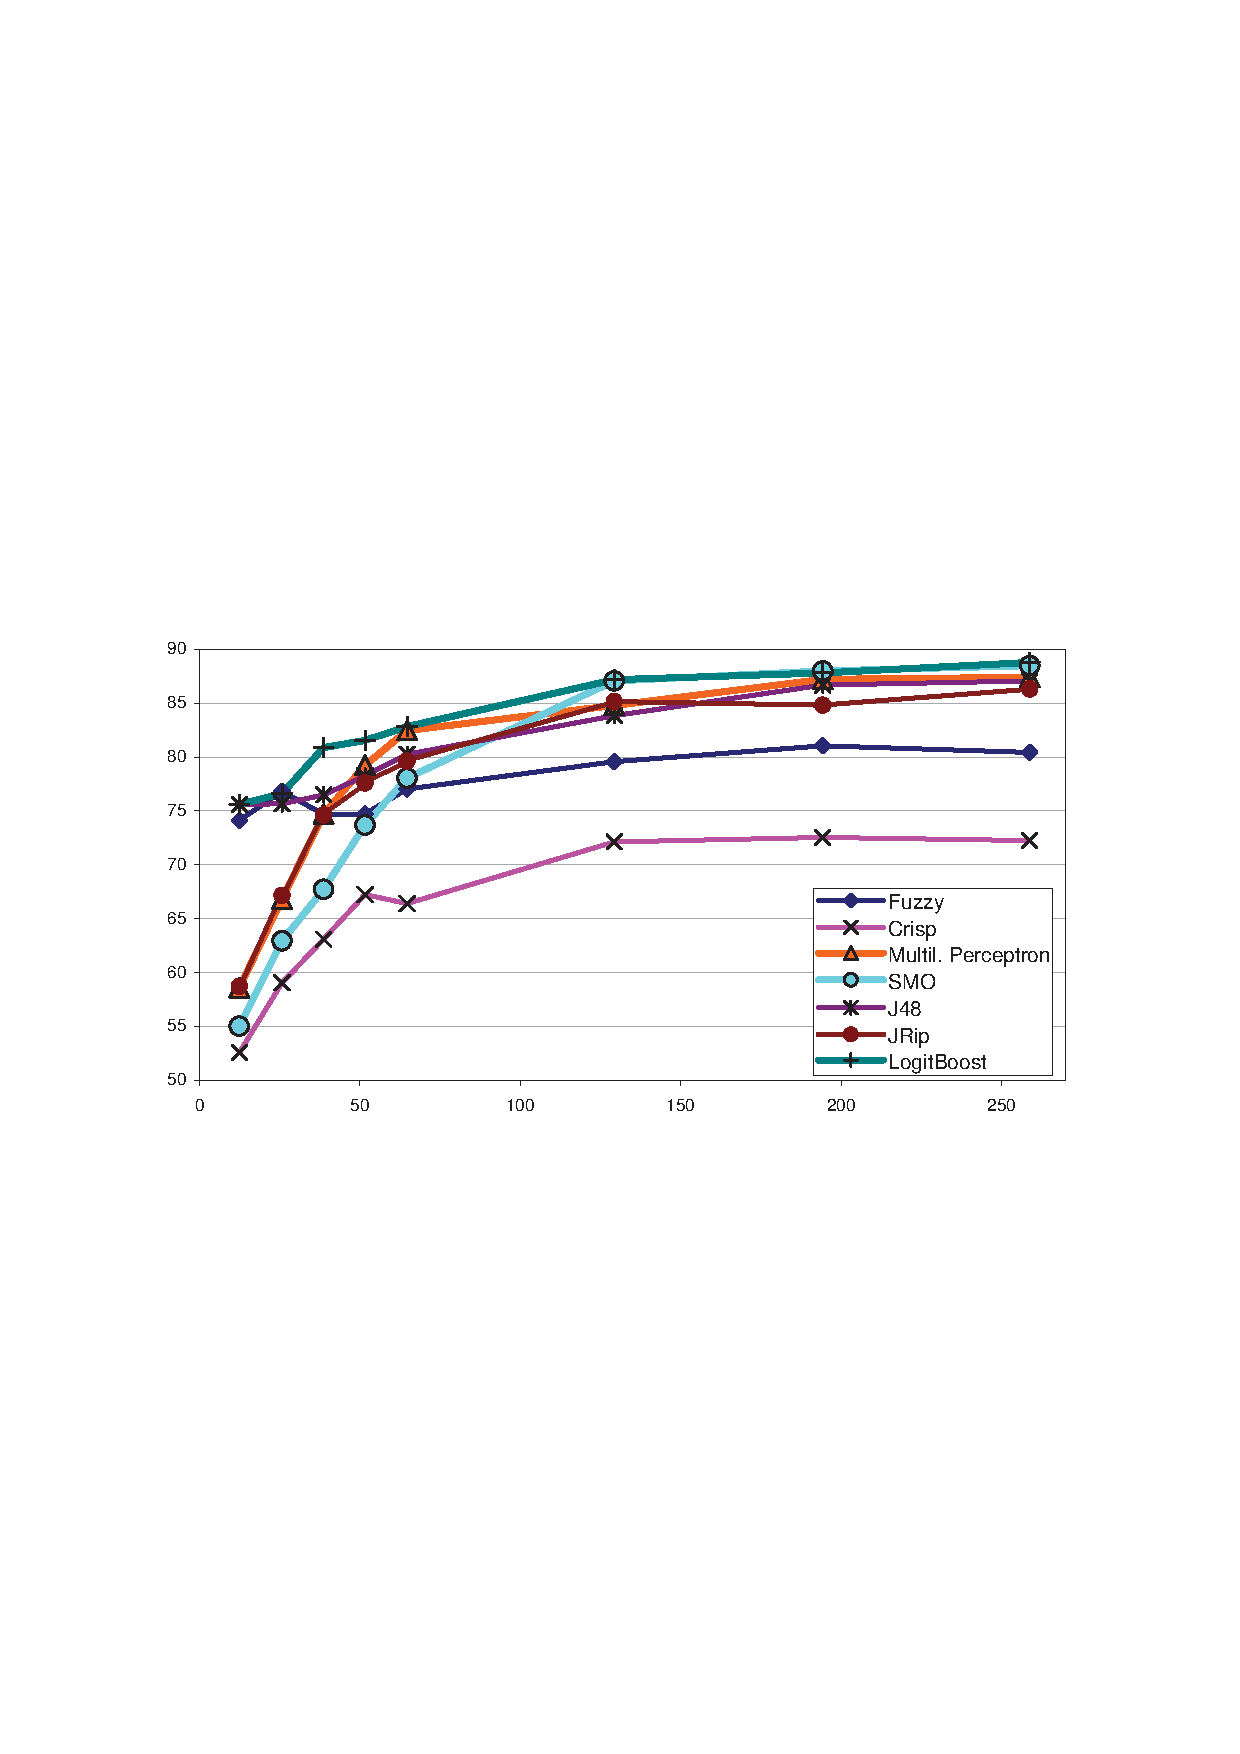
\includegraphics[width=0.8\hsize]{corect_growing_learninig_instances}}
\caption{x-axis: number of training instances, y-axis: percent of correctly classified instances, average values from 10 repetitions, `nursery' dataset.}
\label{fig:corect_growing_learninig_instances}
\end{figure}


\subsection{UCI Time}


Figure~\ref{fig:learning_speed} demonstrates time complexity of the classifiers in the same experiment as in Figure~\ref{fig:corect_growing_learninig_instances}. Despite the fact that the Fuzzy ILP classifier was several times slower than the Crisp ILP classifier and even more than the others, it is still computable on current processors (e.g. P9600, 2.66 GHz, which we used) and the curve of time complexity did not grow rapidly during the experiment. Because ILP is a heuristic and iterative method, the time complexity can be quite directly managed by the setting of learning parameters.

\begin{figure}
\centerline{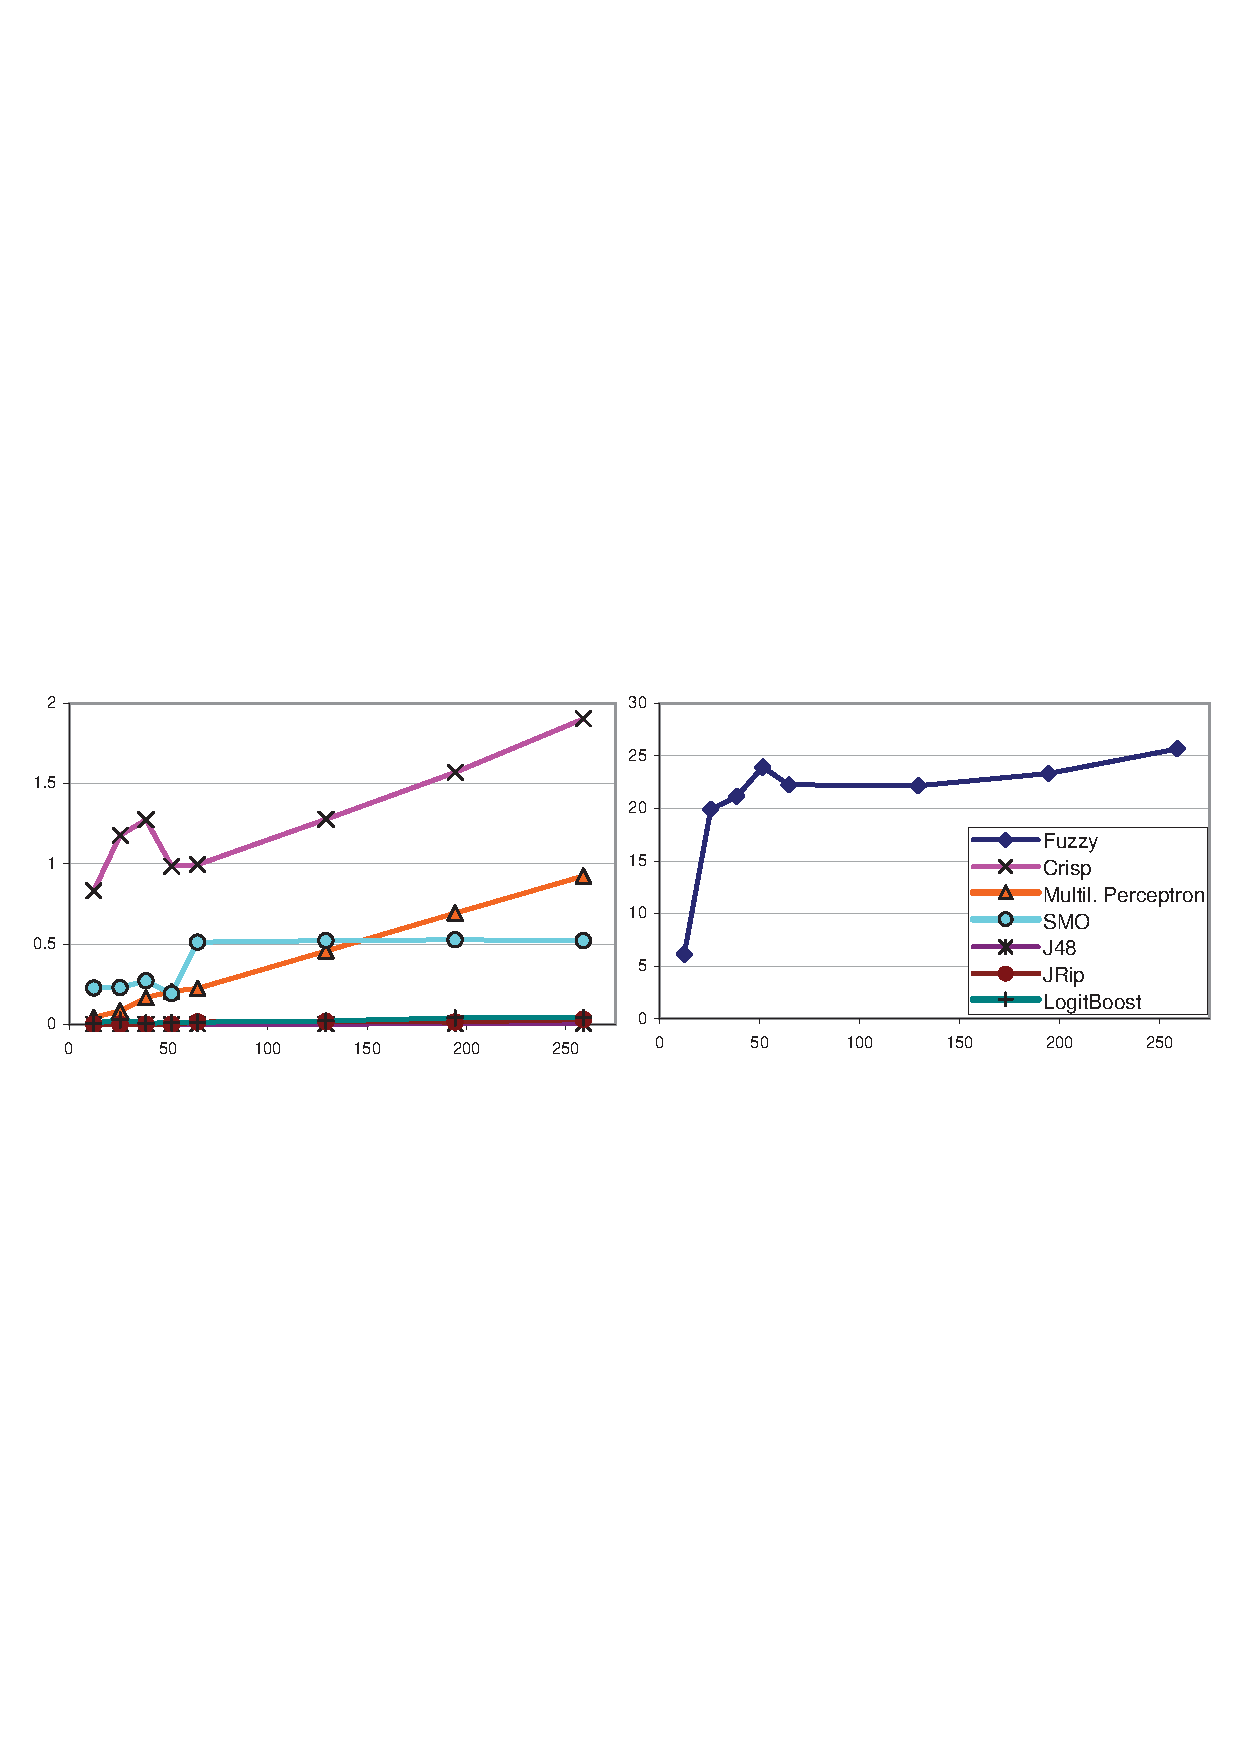
\includegraphics[width=\hsize]{learning_speed}}
\caption{x-axis: number of training instances, y-axis: training time in seconds, average values from 10 repetitions, `nursery' dataset.}
\label{fig:learning_speed}
\end{figure}



\chapter{Conclusion} \label{sec:ch_conclusion}
%\graphicspath{{../img/ch90/}}

This is the last chapter of the thesis. It contains mainly concluding remarks, some additional discussions and an outlook to the future work. First four sections are dedicated to the four main topics of the thesis, followed by common remarks and discussions. 



\section{Manual Design of Extraction Rules}
We have presented the development of our extraction method based on deep language parsing from its early beginning. Its evolution begun with procedurally written extraction rules followed by declarative ones and, finally, it was supported by the automated induction of extraction rules using the machine learning technique of Inductive Logic Programming.


Our extraction method based on manually designed extraction rules do not consider the annotation aspect of information extraction. Although it is possible to infer an annotation based variety of the presented method, we did not take it into account because during the development of the method the aim was more to produce structured data from text than to produce annotated documents. In the second approach the emphasis is inverted. 

A deeper evaluation of the method would be definitely interesting, but at the moment, the information provided is the only available. There is no real world application of the method outside the academic ground. The method is still waiting for deep testing and further development in an extensive real world project.



\section{Machine Learning of Extraction Rules}

From our experiments can be seen that ILP is capable to find complex and meaningful rules that cover the intended information. But in terms of the performance measures the results are not better than those from a propositional learner. This is quite surprising observation mainly for  Czech because it is a language with free word order and we would expect much better results of the dependency based approach than those of the position based approach, which was used by the propositional learner.

Our method is still missing an intelligent semantic interpretation procedure and it could be also evaluated on other datasets (e.g. MUC, ACE, TAC, CoNLL) and other languages. So far we also do not provide a method for classical event and relation extraction. %(like e.g. in \citep{Bunescu:DependencyPaths}). 
In the present solution, we work with events in the same way as with entities; details about this variant of event extraction were provided in Section~\ref{sec:problems_event_entities}. The method has to be adapted for explicit learning of events and relations in the form of ``subject predicate object''.

Our method can also provide a comparison of different linguistic formalisms and tools and their benefit to information extraction because we could run our method using different linguistic analyzers and compare the results on the same dataset.



%%%%%%%%%%%%%%%%%%%%%%%%%%%%%%%%%%%%%%%%%%%%%%%%%%%%%%%%%%%%%%%%%%%%%%%%%%%%%%%%%%%%%%%%%%%%%%%%%%%%%%%%%%%%%%
%%%%%%%%%%%%%%%%%%%%%%%%%%%%%%%%%%%%%%%%%%%%%%%%%%%%%%%%%%%%%%%%%%%%%%%%%%%%%%%%%%%%%%%%%%%%%%%%%%%%%%%%%%%%%%
%%%%%%%%%%%%%%%%%%%%%%%%%%%%%%%%%%%%%%%%%%%%%%%%%%%%%%%%%%%%%%%%%%%%%%%%%%%%%%%%%%%%%%%%%%%%%%%%%%%%%%%%%%%%%%
\section{Shareable Extraction Ontologies} 

%%%%%%%%%%%%%%%%%%%%%%%%%%%%%%%%%%%%%%%%%%%%%%%%%%%%%%%%%%%%%%%%%%%%%%%%%%%%%%%%%%%%%%%%%%%%%%%%%%%%%%%%%%%%%%
\subsection{From Annotations to Real World Facts} \label{sec:onto_discuss}
%%%%%%%%%%%%%%%%%%%%%%%%%%%%%%%%%%%%%%%%%%%%%%%%%%%%%%%%%%%%%%%%%%%%%%%%%%%%%%%%%%%%%%%%%%%%%%%%%%%%%%%%%%%%%%


In this thesis, we have described our method how to apply an extraction ontology to a document ontology and obtain so called ``annotated'' document ontology. To have an ``annotated'' document ontology is almost the same as to have an annotated document. An annotated document is useful (easier navigation, faster reading and lookup of information, possibility of structured queries on collections of such documents, etc.) but if we are interested in the actual information present in the document, if we want to know the facts that are in a document asserted about the real word things then an annotated document is not sufficient. But the conversion of an annotated document to the real world facts is not simple.
There are obvious issues concerning data integration and duplicity of information. For example when in a document two mentions of people are annotated as `injured', what is then the number of injured people in the corresponding accident? Are the two annotations in fact linked to the same person or not?

In the beginning of our work on the idea of shareable extraction ontologies we planned to develop it further, we wanted to cover also the step from annotated document ontologies to the real world facts. The extraction process would then end up with so called ``fact ontologies''. But two main obstacles prevent us to do that.

\begin{enumerate}
	\item Our IE engine is not yet capable to solve these data integration and duplicity of information issues and the real world facts would be quite imprecise then.
	\item There are also technology problems of creating new facts (individuals) during reasoning.
\end{enumerate}

Because of the decidability and finality constraints of the Description Logic Reasoning it is not possible to create new individuals during the reasoning process. There is no standard way how to do it. But there are some proprietary solutions like \verb@swrlx:createOWLThing@\footnote{\url{http://protege.cim3.net/cgi-bin/wiki.pl?action=browse&id=SWRLExtensionsBuiltIns}} from the Prot\'{e}g\'{e} project and \verb@makeTemp(?x)@ or \verb@makeInstance(?x, ?p, ?v)@\footnote{\url{http://jena.sourceforge.net/inference/#RULEbuiltins}} from the Jena project.
And these solutions can be used in the future work. 

\subsection{How to Obtain a Document Ontology?}

It is true that there are standard means how to obtain a (document) ontology from a document, but these means were not intended for a complex transformation of documents to linguistic structures. Also in our case study (Section~\ref{sec:onto_case}), we did not show how the linguistic preprocessing could be embedded in a GRDDL transformation. In fact, our input documents were already linguistically preprocessed before the GRDDL transformation was performed. We can say that this is just a technical problem but it also illustrates that shareable extraction ontologies and probably also extraction ontologies are still rather a vision, however this vision is realizable today.

\subsection{SPARQL Queries -- Increasing Performance?}

There is also a possibility to transform the extraction rules to SPARQL construct queries. This would probably rapidly increase the time performance. However a document ontology would then have to exactly fit with the schema of the extraction rules.  This would be a minor problem. 

The reason why we did not study this approach from the beginning is that we were interested in extraction \emph{ontologies} and SPARQL queries are not currently regarded as a part of an ontology and nothing is suggesting it to be that way.  

Anyway the performance comparison remains a valuable task for the future work.

\subsection{Contributions for Information Extraction}

Our work on extraction ontologies combines the field of ontology-based information extraction and rule-based reasoning. The aim is to show a new possibility in usage of IE tools and reasoners. The idea of shareable extraction ontologies do not bring a solution that would improve the performance of IE tools.

We also do not provide a proposal of a universal extraction ontology format (although a specific form for the rule based extraction on dependency parsed text could be inferred). This task is left for the future if a need for such activity emerges.
%The aim of the chapter is a demonstration of the idea of tool independent extraction ontologies and the possibility to use reasoners for information extraction.


%%%%%%%%%%%%%%%%%%%%%%%%%%%%%%%%%%%%%%%%%%%%%%%%%%%%%%%%%%%%%%%%%%%%%%%%%%%%%%%%%%%%%%%%%%%%%%%%%%%%%%%%%%%%%%
\subsection{Summary} \label{sec:onto_conclusion}
%%%%%%%%%%%%%%%%%%%%%%%%%%%%%%%%%%%%%%%%%%%%%%%%%%%%%%%%%%%%%%%%%%%%%%%%%%%%%%%%%%%%%%%%%%%%%%%%%%%%%%%%%%%%%%

%In the end of the chapter we would like to summarize the main contributions of the chapter.

%\begin{itemize}
	%\item In the beginning of the chapter we pointed out the draw back of so called extraction ontologies -- in most cases they are dependent on a particular extraction/annotation tool and they cannot be used separately.	
	%\item We extended the concept of extraction ontologies by adding the shareable aspect and we introduced a new principle of making extraction ontologies independent of the original tool: the possibility of application of an extraction ontology to a document by an ordinary reasoner.
	%\item In Section~\ref{sec:onto_case} we presented a case study that shows that the idea of shareable extraction ontologies is realizable. We presented implementation of an IE tool that exports its extraction rules to an extraction ontology and we demonstrated how this extraction ontology can be applied to a document by a reasoner.
	%\item Moreover in Section~\ref{sec:onto_experiment} an experiment with several OWL reasoners was presented. The experiment evaluated the performance of contemporary OWL reasoners on IE tasks (application of extraction ontologies).  
	%\item A new publically available benchmark for OWL reasoning was created together with the experiment. Other reasoners can be tested this way.
%\end{itemize}
   
In the beginning of the description of shareable extraction ontologies, we pointed out the draw back of so called extraction ontologies -- in most cases they are dependent on a particular extraction/annotation tool and they cannot be used separately.	

We extended the concept of extraction ontologies by adding the shareable aspect and we introduced a new principle of making extraction ontologies independent of the original tool: the possibility of application of an extraction ontology to a document by an ordinary reasoner.

In Section~\ref{sec:onto_case} we presented a case study that shows that the idea of shareable extraction ontologies is realizable. We presented implementation of our IE tool that exports its extraction rules to an extraction ontology and we demonstrated how this extraction ontology can be applied to a document by a reasoner.

Moreover in Section~\ref{sec:onto_experiment} an experiment with several OWL reasoners was presented. The experiment evaluated the performance of contemporary OWL reasoners on IE tasks (application of extraction ontologies). A new publically available benchmark for OWL reasoning was created together with the experiment. Other reasoners can be tested this way.

%We would like to conclude the chapter by stating that only time will show if the fundamental idea of the chapter will be useful but today it is at least a new use case for both: usage of IE tools and reasoners.



%%%%%%%%%%%%%%%%%%%%%%%%%%%%%%%%%%%%%%%%%%%%%%%%%%%%%%%%%%%%%%%%%%%%%%%%%%%%%%%%%%%%%%%%%%%%%%%%%
%%%%%%%%%%%%%%%%%%%%%%%%%%%%%%%%%%%%%%%%%%%%%%%%%%%%%%%%%%%%%%%%%%%%%%%%%%%%%%%%%%%%%%%%%%%%%%%%%
%%%%%%%%%%%%%%%%%%%%%%%%%%%%%%%%%%%%%%%%%%%%%%%%%%%%%%%%%%%%%%%%%%%%%%%%%%%%%%%%%%%%%%%%%%%%%%%%%
\section{Fuzzy ILP Classification} \label{sec:conclusion}


In our work on fuzzy ILP classification, we provided a design and partial implementation of a fuzzy system, which provides a fuzzy classification of textual reports. Our approach is based on usage of third party linguistic analyzers, our work on information extraction, and fuzzy inductive logic programming.

The main contributions are formal models, prototype implementation of the presented methods and evaluation experiments. The first experiment evaluated performance of the presented methods and compared them with other machine learning procedures used in data mining on our dataset. The Fuzzy ILP Classifier proved better results than a majority of the methods. The results are statistically significant in many cases. 
We see the advantage of the Fuzzy ILP classifier in the fact that monotonization leads to the extension of the learning domain and it utilizes the fact that the domain is or can be monotonically ordered.

In the second experiment, we evaluated all the methods on other datasets with more training instances and we also experimentally measured the time complexity of the methods. This experiment shows that the fuzzy method is suitable mainly in situations with a small amount of training instances and in cases when the target attribute mostly respects the natural order of the remaining attributes. But this did not hold true for any of the later-used datasets. When comparing the fuzzy approach with the crisp one, the fuzzy approach always performed better in terms of correctness of the classification, but it was many times slower than all the methods in terms of time complexity.



\section{Statistical Significance} \label{sec:conclusion_statsig}
The term statistical significance used in this thesis refers to the result of a pair-wise comparison of learning engines using the corrected resampled (two tailed) T-Test \citep{Nadeau:2003:IGE:779909.779927}, which is suitable for cross validation based experiments. The Weka implementation was used (see some details in Section~\ref{sec:third_weka}). Test significance was 0.05 in all cases.




\section{How to Download} \label{sec:download_notes}
The project website\footnote{\url{http://czsem.berlios.de}} provides several ways how to get all the presented tools running. A platform independent installer, Java binaries and source codes are provided under the GPL license.

Also majority of the datasets mentioned in this thesis are available for public download.

Table~\ref{tab:download_links} provides links to individual resources.


\begin{table}
\centering
\begin{tabular}{|p{.97\textwidth}|}
		\hline
		Czsem Mining Suite installation: \hfill{} \smallurl{http://czsem.berlios.de/czsem_install.html}\\
		\hline
		Fuzzy ILP Classifier for Weka:  \hfill{} \smallurl{http://www.ksi.mff.cuni.cz/~dedek/fuzzyILP/}\\
		\hline
		Ontologies: \hfill{}\\
		$\,$\hfill{} \smallurl{http://czsem.berlios.de/ontologies/acquisitions-v1.1/download_instructions.html}\\
		$\,$\hfill{} \smallurl{http://czsem.berlios.de/ontologies/czech_fireman/download_instructions.html}\\
		\hline		
		General download area: \hfill{}\\
		$\,$\hfill{} \smallurl{http://developer.berlios.de/project/filelist.php?group_id=8427}\\
		\hline
		Apache Maven repository: \hfill{} \smallurl{http://czsem.berlios.de/maven2/}\\
		\hline 
\end{tabular}
	\caption{Download links to the implementation and datasets.} \label{tab:download_links}
\end{table}

\section{Repeatability of Experiments} \label{sec:conclusion_repeatablity}

Our implementation and datasets are publicly available. This makes our experiments repeatable according to the
SIGMOD Experimental Repeatability Requirements \citep{biblio:SIGMODrepeatability}. If you have any problems concerning the reconstruction of any of the experiments please contact the authors, they will pleased by providing an assistance. 



\section{Summary}

Our experiments deal with texts in the Czech language but our method is general and it can be used with any structured linguistic representation. 

 



%%% Seznam použité literatury
\myaddchaptertoc{Bibliography}
\bibliographystyle{../style/iisproc}
\bibliography{../dedek_phd}


%\chapwithtoc{List of Figures}
\myaddchaptertoc{List of Figures}
\listoffigures


%%% Tabulky v disertační práci, existují-li.
%\chapwithtoc{List of Tables}
\myaddchaptertoc{List of Tables}
\listoftables

%%% Použité zkratky v disertační práci, existují-li, včetně jejich vysvětlení.
%\chapwithtoc{List of Abbreviations}
\myaddchaptertoc{Nomenclature}
\nomenclature{API}{Application Programming Interface}

\nomenclature{FS}{Feature Structure}

\nomenclature{GPL}{GNU General Public License \\\url{http://www.gnu.org/licenses/gpl.html}}

\nomenclature{GRDDL}{Gleaning Resource Descriptions from Dialects of Languages \\\url{http://www.w3.org/TR/grddl/}}

\nomenclature{IE}{Information Extraction}

\nomenclature{ILP}{Inductive Logic Programming}

\nomenclature{JAPE}{Java Annotation Patterns Engine \\\url{http://gate.ac.uk/userguide/chap:jape}}

\nomenclature{ML}{Machine Learning}

\nomenclature{OWL}{Web Ontology Language \\\url{http://www.w3.org/TR/owl-primer/}}

\nomenclature{PAUM}{Perceptron Algorithm with Uneven Margins}

\nomenclature{PML}{Prague Markup Language}

\nomenclature{PDT}{Prague Dependency Treebank}

\nomenclature{RDFa}{Resource Description Framework - in - attributes \\\url{http://www.w3.org/TR/xhtml-rdfa-primer/}}

\nomenclature{RDF}{Resource Description Framework \\\url{http://www.w3.org/RDF/}}

\nomenclature{RPC}{Remote Procedure Call}

\nomenclature{RSS}{Really Simple Syndication, or Rich Site Summary, but originally RDF Site Summary \\\url{http://www.rssboard.org/rss-specification}}

\nomenclature{SPARQL}{SPARQL Query Language for RDF \\\url{http://www.w3.org/TR/rdf-sparql-query/}}

\nomenclature{SQL}{Structured Query Language \\\url{http://www.iso.org/iso/catalogue_detail.htm?csnumber=45498}}

\nomenclature{URL}{Uniform Resource Locator \\(RFC1738 \url{http://www.ietf.org/rfc/rfc1738.txt})}


\nomenclature{XML}{Extensible Markup Language \\\url{http://www.w3.org/XML/}}

\nomenclature{XSLT}{Extensible Stylesheet Language Transformations \\\url{http://www.w3.org/TR/xslt}}


\printnomenclature[2.5cm]

%%% Přílohy k disertační práci, existují-li (různé dodatky jako výpisy programů,
%%% diagramy apod.). Každá příloha musí být alespoň jednou odkazována z vlastního
%%% textu práce. Přílohy se číslují.


%\chapwithtoc{Attachments}
\appendix


\chapter{Listings}
Individual listings are placed as separate sections on following pages.

\clearpage
\section{Sample of Czech WordNet}	\label{sec:listing_czWordNet}
This sample shows the word coverage in the domain of means of transport and vehicles. We do not provide the complete transcript of Czech words. The top subtree demonstrates the distance between the words ``autobus, autokar'' (bus, coach) and ``kamion'' (truck) in the hypernym hierarchy and the rest of the sample lists all hyponyms of the three selected words: ``motorové vozidlo'' (motor vehicle), ``nákladní automobil'' (truck) and ``auto, vůz'' (car).

\bigskip

\fbox{\parbox[b]{\hsize}{
\hspace*{0cm}$\bullet$ entita:1\\
\hspace*{1cm}$\bullet$ objekt:1\\
\hspace*{2cm}$\bullet$ celek:1\\
\hspace*{3cm}$\bullet$ artefakt:1, výtvor:2, výrobek:2\\
\hspace*{4cm}$\bullet$ vybavení:2\\
\hspace*{5cm}$\bullet$ přepravní prostředek:1, transportní prostředek:1\\
\hspace*{6cm}$\triangleright$ \textbf{veřejná doprava:1}\\
\hspace*{7cm}$\Rightarrow$ \emph{autobus:1, autokar:1}\\
\hspace*{6cm}$\triangleright$ \textbf{dopravní prostředek:1}\\
\hspace*{7cm}$\bullet$ kolové vozidlo:1\\
\hspace*{8cm}$\bullet$ samohybné vozidlo:1,\\
\hspace*{8cm}\phantom{$\bullet$} vozidlo s vlastním pohonem:1\\
\hspace*{9cm}$\bullet$ motorové vozidlo:1\\
\hspace*{10cm}$\bullet$ nákladní automobil:1\\
\hspace*{11cm}$\Rightarrow$ \emph{kamion:1}

\vspace{0.5cm}

\setlength{\columnsep}{0cm}

\begin{multicols}{2}

\hspace*{0cm}$\bullet$ motorové vozidlo:1\\
\hspace*{1cm}$\bullet$ motocykl:1\\
\hspace*{1cm}$\bullet$ nákladní automobil:1\\
\hspace*{1cm}$\bullet$ obojživelné vozidlo:1\\
\hspace*{1cm}$\bullet$ auto:1, vůz:2\\
\hspace*{1cm}$\bullet$ pohřební vůz:1\\
\hspace*{1cm}$\bullet$ sněžný pluh:1, pluh:2\\
\hspace*{1cm}$\bullet$ golfový vozík:1\\

\vspace{0.5cm}

\hspace*{0cm}$\bullet$ nákladní automobil:1\\
\hspace*{1cm}$\bullet$ dodávka:3\\
\hspace*{1cm}$\bullet$ sklápěč:1,\\
\hspace*{1cm}\phantom{$\bullet$}  vyklápěcí nákladní automobil:1\\
\hspace*{1cm}$\bullet$ tahač:1\\
\hspace*{1cm}$\bullet$ pick-up:1, malý nákladní automobil:1\\
\hspace*{1cm}$\bullet$ hasící vůz:1, požární stříkačka:1\\
\hspace*{1cm}$\bullet$ rozhlasový vůz:1\\
\hspace*{1cm}$\bullet$ kamion:1\\
\hspace*{1cm}$\bullet$ nákladní automobil s přívěsem:1\\
\hspace*{1cm}$\bullet$ popelářský vůz:1, popelářské auto:1,\\
\hspace*{1cm}\phantom{$\bullet$} bobr:3\\

\columnbreak

\hspace*{0cm}$\bullet$ auto:1, vůz:2\\
\hspace*{1cm}$\bullet$ limuzína:1\\
\hspace*{1cm}$\bullet$ elektrický vozík:1\\
\hspace*{1cm}$\bullet$ závodní vůz:1, závodní automobil:1\\
\hspace*{1cm}$\bullet$ sportovní vůz:1\\
\hspace*{1cm}$\bullet$ kabriolet:1, sporťák:1\\
\hspace*{1cm}$\bullet$ vrak:3\\
\hspace*{1cm}$\bullet$ limuzína:2\\
\hspace*{1cm}$\bullet$ hlídkový vůz:1, policejní vůz:1\\
\hspace*{1cm}$\bullet$ sériový automobil:1\\
\hspace*{1cm}$\bullet$ cestovní vůz:1\\
\hspace*{1cm}$\bullet$ džíp:1\\
\hspace*{1cm}$\bullet$ kupé:1\\
\hspace*{1cm}$\bullet$ kabriolet:3\\
\hspace*{1cm}$\bullet$ kombi:1\\
\hspace*{1cm}$\bullet$ taxi:1\\
\hspace*{1cm}$\bullet$ ambulance:1, sanitka:1,\\
\hspace*{1cm}\phantom{$\bullet$} pohotovost:6, záchranka:1, sanita:1
\end{multicols}
\setlength{\columnsep}{5cm}
}}


\clearpage
\section{Extraction rules export to OWL in Prolog.} \label{sec:onto_prolog_rules_export_module}
\begin{minted}[linenos,  fontsize=\footnotesize,
               frame=lines, tabsize=2]{prolog}
serialize_rule_file(RuleFileName, OutputFileName, OntologyURI, ObjectProperties) :-
	assert(objectProperties(ObjectProperties)),
	open(OutputFileName, 'write', Stream), set_output(Stream),
	write('<?xml version="1.0" encoding="UTF-8"?>\n'),
	write('<!DOCTYPE Ontology [ <!ENTITY xsd "http://www.w3.org/2001/XMLSchema#" >\n'),
	write('	<!ENTITY pml "http://ufal.mff.cuni.cz/pdt/pml/" > ]>\n'),		
	write('<Ontology xmlns="http://www.w3.org/2002/07/owl#"\n'),	
	format('	ontologyIRI="~a">\n',[OntologyURI]),
	consult(RuleFileName), %Each rule in the file will be processed by serialize_rule,
	                       %because of the term_expansion setting on the last line. 	                         
	write('</Ontology>'),			
	close(Stream).

serialize_rule(:-(H, B)) :- 	
	numbervars(:-(H, B), 0, _),	
	write('<DLSafeRule>\n'),		
		write('<Body>\n'),          
			serialize_term(B),                       %Rule body
		write('\n</Body>\n'), write('<Head>\n'),
			serialize_term(H),                       %Rule head
		write('\n</Head>\n'),			
	write('</DLSafeRule>\n\n'),!.
	 
%Serialize object property
serialize_term(T):- functor(T,F,N), objectProperties(OProps), member(F, OProps),!,	
	write('<ObjectPropertyAtom>'),
	format('<ObjectProperty IRI="&pml;~a"/>\n', [F]),
	serialize_arg(T, 0, N),		
	write('</ObjectPropertyAtom>').

%Serialize datatype property
serialize_term(T):- functor(T,F,N),	
	write('<DataPropertyAtom>'),
	format('<DataProperty IRI="&pml;~a"/>\n', [F]),
	serialize_arg(T, 0, N),		
	write('</DataPropertyAtom>').

%Serialize argument list
serialize_term(','(A,B)):- serialize_term(A), write('\n'), serialize_term(B),!.

%Serialize variable
serialize_term('$VAR'(N)):- char_code('a',I), Var is I + N,
	format('<Variable IRI="urn:swrl#~c"/>\n',[Var]),!.
%Serialize simple atom or string (printed without quotes)
serialize_term(T):- atom(T), format('<Literal>~a</Literal>\n',[T]),!.
%Serialize number
serialize_term(T):- simple(T), format('<Literal>~k</Literal>\n',[T]),!.

%Serialize term arguments: serialize_arg(+Term, +CurrentArgNumber, +LastArgNumber)
serialize_arg(T, _, 0).
serialize_arg(T, N, N).
serialize_arg(T, M, N) :-  M2 is M+1, arg(M2, T, A),
	serialize_term(A), serialize_arg(T, M2, N).  
                                               %All predicates loaded by consult
term_expansion(T,T):- serialize_rule(T).       %will be processed by serialize_rule.
\end{minted}



\chapter{Complete Evaluation Results}

\section{Czech Fireman}

\begin{longtable}{|r|r|l||rcl|rcl|c|}
\hline
\multirow{2}{*}{task} & \multicolumn{2}{|c||}{\multirow{2}{*}{measured quantity}} & \multicolumn{3}{|c|}{ILP} & \multicolumn{3}{|c|}{PAUM} & \multirow{2}{*}{ stat. sig.}\\
\cline{4-9}
  & \multicolumn{2}{|c||}{} &  avg  &    &  stdev  &  avg  &    &  stdev  & \\
\hline
\endhead
\hline
\hline
\multirow{11}{*}{\begin{sideways}damage\end{sideways} }
             & \multirow{4}{*}{    Number} &         Correct &       2.250 &  $\pm$  &       1.164 &       2.000 &  $\pm$  &       1.091 & $\bullet$ \\
\cline{3-10} &                             &         Missing &       0.250 &  $\pm$  &       0.436 &       0.500 &  $\pm$  &       0.656 & $\circ$ \\
\cline{3-10} &                             &        Spurious &       0.613 &  $\pm$  &       1.000 &       0.288 &  $\pm$  &       0.556 & $\bullet$ \\
\cline{3-10} &                             &         Overlap &       0.000 &  $\pm$  &       0.000 &       0.000 &  $\pm$  &       0.000 &  \\
\cline{2-10} & \multirow{3}{*}{    Strict} &       Precision &       0.853 &  $\pm$  &       0.193 &       0.913 &  $\pm$  &       0.160 & $\circ$ \\
\cline{3-10} &                             &          Recall &       0.904 &  $\pm$  &       0.188 &       0.817 &  $\pm$  &       0.258 & $\bullet$ \\
\cline{3-10} &                             &           $F_1$ &       0.848 &  $\pm$  &       0.169 &       0.824 &  $\pm$  &       0.224 &  \\
\cline{2-10} &                     Lenient &           $F_1$ &       0.848 &  $\pm$  &       0.169 &       0.824 &  $\pm$  &       0.224 &  \\
\cline{2-10} &                     Average &           $F_1$ &       0.848 &  $\pm$  &       0.169 &       0.824 &  $\pm$  &       0.224 &  \\
\cline{2-10} & \multirow{2}{*}{    Number} &   Training Inst &    \multicolumn{3}{c|}{n/a}         &      17.500 &  $\pm$  &       1.180 &  \\
\cline{3-10} &                             &   Training Docs &    \multicolumn{3}{c|}{n/a}         &      43.750 &  $\pm$  &       0.436 &  \\
\cline{2-10} & \multirow{2}{*}{      Time} &        Training &      0:02.2 &  $\pm$  &      0:00.1 &      0:24.1 &  $\pm$  &      0:06.3 & $\circ$ \\
\cline{3-10} &                             &         Testing &      0:00.3 &  $\pm$  &      0:00.1 &      0:00.9 &  $\pm$  &      0:00.2 & $\circ$ \\
\hline
\hline
\multirow{11}{*}{\begin{sideways}end subtree\end{sideways} }
             & \multirow{4}{*}{    Number} &         Correct &       3.200 &  $\pm$  &       1.444 &       1.313 &  $\pm$  &       1.051 & $\bullet$ \\
\cline{3-10} &                             &         Missing &       1.575 &  $\pm$  &       1.271 &       3.713 &  $\pm$  &       1.759 & $\circ$ \\
\cline{3-10} &                             &        Spurious &       2.775 &  $\pm$  &       1.669 &       0.775 &  $\pm$  &       1.043 & $\bullet$ \\
\cline{3-10} &                             &         Overlap &       0.475 &  $\pm$  &       0.693 &       0.225 &  $\pm$  &       0.595 & $\bullet$ \\
\cline{2-10} & \multirow{3}{*}{    Strict} &       Precision &       0.510 &  $\pm$  &       0.210 &       0.689 &  $\pm$  &       0.317 & $\circ$ \\
\cline{3-10} &                             &          Recall &       0.623 &  $\pm$  &       0.226 &       0.254 &  $\pm$  &       0.214 & $\bullet$ \\
\cline{3-10} &                             &           $F_1$ &       0.541 &  $\pm$  &       0.192 &       0.312 &  $\pm$  &       0.222 & $\bullet$ \\
\cline{2-10} &                     Lenient &           $F_1$ &       0.618 &  $\pm$  &       0.174 &       0.357 &  $\pm$  &       0.244 & $\bullet$ \\
\cline{2-10} &                     Average &           $F_1$ &       0.579 &  $\pm$  &       0.174 &       0.335 &  $\pm$  &       0.225 & $\bullet$ \\
\cline{2-10} & \multirow{2}{*}{    Number} &   Training Inst &    \multicolumn{3}{c|}{n/a}         &      36.750 &  $\pm$  &       1.852 &  \\
\cline{3-10} &                             &   Training Docs &    \multicolumn{3}{c|}{n/a}         &      43.750 &  $\pm$  &       0.436 &  \\
\cline{2-10} & \multirow{2}{*}{      Time} &        Training &      0:02.2 &  $\pm$  &      0:00.1 &      1:37.8 &  $\pm$  &      0:14.6 & $\circ$ \\
\cline{3-10} &                             &         Testing &      0:00.3 &  $\pm$  &      0:00.1 &      0:00.9 &  $\pm$  &      0:00.2 & $\circ$ \\
\hline
\hline
\multirow{11}{*}{\begin{sideways}start\end{sideways} }
             & \multirow{4}{*}{    Number} &         Correct &       5.150 &  $\pm$  &       0.969 &       4.725 &  $\pm$  &       1.125 & $\bullet$ \\
\cline{3-10} &                             &         Missing &       0.100 &  $\pm$  &       0.302 &       0.525 &  $\pm$  &       0.656 & $\circ$ \\
\cline{3-10} &                             &        Spurious &       2.950 &  $\pm$  &       1.466 &       0.388 &  $\pm$  &       0.684 & $\bullet$ \\
\cline{3-10} &                             &         Overlap &       0.000 &  $\pm$  &       0.000 &       0.000 &  $\pm$  &       0.000 &  \\
\cline{2-10} & \multirow{3}{*}{    Strict} &       Precision &       0.654 &  $\pm$  &       0.117 &       0.936 &  $\pm$  &       0.103 & $\circ$ \\
\cline{3-10} &                             &          Recall &       0.980 &  $\pm$  &       0.061 &       0.896 &  $\pm$  &       0.130 & $\bullet$ \\
\cline{3-10} &                             &           $F_1$ &       0.779 &  $\pm$  &       0.087 &       0.909 &  $\pm$  &       0.094 & $\circ$ \\
\cline{2-10} &                     Lenient &           $F_1$ &       0.779 &  $\pm$  &       0.087 &       0.909 &  $\pm$  &       0.094 & $\circ$ \\
\cline{2-10} &                     Average &           $F_1$ &       0.779 &  $\pm$  &       0.087 &       0.909 &  $\pm$  &       0.094 & $\circ$ \\
\cline{2-10} & \multirow{2}{*}{    Number} &   Training Inst &    \multicolumn{3}{c|}{n/a}         &      36.750 &  $\pm$  &       0.907 &  \\
\cline{3-10} &                             &   Training Docs &    \multicolumn{3}{c|}{n/a}         &      43.750 &  $\pm$  &       0.436 &  \\
\cline{2-10} & \multirow{2}{*}{      Time} &        Training &      0:02.2 &  $\pm$  &      0:00.1 &      0:26.5 &  $\pm$  &      0:04.1 & $\circ$ \\
\cline{3-10} &                             &         Testing &      0:00.3 &  $\pm$  &      0:00.0 &      0:00.9 &  $\pm$  &      0:00.1 & $\circ$ \\
\hline
\pagebreak[4]
\hline
\hline
\multirow{11}{*}{\begin{sideways}injuries\end{sideways} }
             & \multirow{4}{*}{    Number} &         Correct &       2.963 &  $\pm$  &       1.958 &       1.875 &  $\pm$  &       1.546 & $\bullet$ \\
\cline{3-10} &                             &         Missing &       1.163 &  $\pm$  &       1.479 &       2.250 &  $\pm$  &       1.886 & $\circ$ \\
\cline{3-10} &                             &        Spurious &       5.200 &  $\pm$  &       3.793 &       1.613 &  $\pm$  &       1.355 & $\bullet$ \\
\cline{3-10} &                             &         Overlap &       0.000 &  $\pm$  &       0.000 &       0.000 &  $\pm$  &       0.000 &  \\
\cline{2-10} & \multirow{3}{*}{    Strict} &       Precision &       0.394 &  $\pm$  &       0.268 &       0.559 &  $\pm$  &       0.325 & $\circ$ \\
\cline{3-10} &                             &          Recall &       0.801 &  $\pm$  &       0.242 &       0.540 &  $\pm$  &       0.322 & $\bullet$ \\
\cline{3-10} &                             &           $F_1$ &       0.470 &  $\pm$  &       0.251 &       0.484 &  $\pm$  &       0.288 &  \\
\cline{2-10} &                     Lenient &           $F_1$ &       0.470 &  $\pm$  &       0.251 &       0.484 &  $\pm$  &       0.288 &  \\
\cline{2-10} &                     Average &           $F_1$ &       0.470 &  $\pm$  &       0.251 &       0.484 &  $\pm$  &       0.288 &  \\
\cline{2-10} & \multirow{2}{*}{    Number} &   Training Inst &    \multicolumn{3}{c|}{n/a}         &      28.875 &  $\pm$  &       2.874 &  \\
\cline{3-10} &                             &   Training Docs &    \multicolumn{3}{c|}{n/a}         &      43.750 &  $\pm$  &       0.436 &  \\
\cline{2-10} & \multirow{2}{*}{      Time} &        Training &      0:02.2 &  $\pm$  &      0:00.1 &      1:34.9 &  $\pm$  &      0:15.2 & $\circ$ \\
\cline{3-10} &                             &         Testing &      0:00.3 &  $\pm$  &      0:00.0 &      0:00.9 &  $\pm$  &      0:00.1 & $\circ$ \\
\hline
\hline
\multirow{11}{*}{\begin{sideways}fatalities\end{sideways} }
             & \multirow{4}{*}{    Number} &         Correct &       0.513 &  $\pm$  &       0.779 &       0.200 &  $\pm$  &       0.403 & $\bullet$ \\
\cline{3-10} &                             &         Missing &       0.863 &  $\pm$  &       1.040 &       1.175 &  $\pm$  &       1.145 & $\circ$ \\
\cline{3-10} &                             &        Spurious &       1.575 &  $\pm$  &       1.403 &       0.225 &  $\pm$  &       0.636 & $\bullet$ \\
\cline{3-10} &                             &         Overlap &       0.000 &  $\pm$  &       0.000 &       0.000 &  $\pm$  &       0.000 &  \\
\cline{2-10} & \multirow{3}{*}{    Strict} &       Precision &       0.347 &  $\pm$  &       0.401 &       0.863 &  $\pm$  &       0.335 & $\circ$ \\
\cline{3-10} &                             &          Recall &       0.567 &  $\pm$  &       0.452 &       0.417 &  $\pm$  &       0.451 & $\bullet$ \\
\cline{3-10} &                             &           $F_1$ &       0.221 &  $\pm$  &       0.309 &       0.346 &  $\pm$  &       0.431 & $\circ$ \\
\cline{2-10} &                     Lenient &           $F_1$ &       0.221 &  $\pm$  &       0.309 &       0.346 &  $\pm$  &       0.431 & $\circ$ \\
\cline{2-10} &                     Average &           $F_1$ &       0.221 &  $\pm$  &       0.309 &       0.346 &  $\pm$  &       0.431 & $\circ$ \\
\cline{2-10} & \multirow{2}{*}{    Number} &   Training Inst &    \multicolumn{3}{c|}{n/a}         &       9.625 &  $\pm$  &       1.205 &  \\
\cline{3-10} &                             &   Training Docs &    \multicolumn{3}{c|}{n/a}         &      43.750 &  $\pm$  &       0.436 &  \\
\cline{2-10} & \multirow{2}{*}{      Time} &        Training &      0:02.2 &  $\pm$  &      0:00.1 &      0:45.5 &  $\pm$  &      0:09.0 & $\circ$ \\
\cline{3-10} &                             &         Testing &      0:00.3 &  $\pm$  &      0:00.1 &      0:00.9 &  $\pm$  &      0:00.2 & $\circ$ \\
\hline
\hline
\multirow{11}{*}{\begin{sideways}profesional unit\end{sideways} }
             & \multirow{4}{*}{    Number} &         Correct &       7.763 &  $\pm$  &       1.918 &       4.863 &  $\pm$  &       1.798 & $\bullet$ \\
\cline{3-10} &                             &         Missing &       1.175 &  $\pm$  &       1.597 &       2.838 &  $\pm$  &       2.089 & $\circ$ \\
\cline{3-10} &                             &        Spurious &       3.375 &  $\pm$  &       2.218 &       3.463 &  $\pm$  &       2.210 &  \\
\cline{3-10} &                             &         Overlap &       0.813 &  $\pm$  &       0.929 &       2.050 &  $\pm$  &       1.349 & $\circ$ \\
\cline{2-10} & \multirow{3}{*}{    Strict} &       Precision &       0.674 &  $\pm$  &       0.132 &       0.500 &  $\pm$  &       0.189 & $\bullet$ \\
\cline{3-10} &                             &          Recall &       0.814 &  $\pm$  &       0.156 &       0.500 &  $\pm$  &       0.152 & $\bullet$ \\
\cline{3-10} &                             &           $F_1$ &       0.730 &  $\pm$  &       0.126 &       0.488 &  $\pm$  &       0.154 & $\bullet$ \\
\cline{2-10} &                     Lenient &           $F_1$ &       0.799 &  $\pm$  &       0.104 &       0.686 &  $\pm$  &       0.114 & $\bullet$ \\
\cline{2-10} &                     Average &           $F_1$ &       0.765 &  $\pm$  &       0.109 &       0.587 &  $\pm$  &       0.121 & $\bullet$ \\
\cline{2-10} & \multirow{2}{*}{    Number} &   Training Inst &    \multicolumn{3}{c|}{n/a}         &      92.750 &  $\pm$  &       3.128 &  \\
\cline{3-10} &                             &   Training Docs &    \multicolumn{3}{c|}{n/a}         &      43.750 &  $\pm$  &       0.436 &  \\
\cline{2-10} & \multirow{2}{*}{      Time} &        Training &      0:02.2 &  $\pm$  &      0:00.1 &      2:41.4 &  $\pm$  &      0:24.5 & $\circ$ \\
\cline{3-10} &                             &         Testing &      0:00.3 &  $\pm$  &      0:00.0 &      0:00.9 &  $\pm$  &      0:00.1 & $\circ$ \\
\hline
\pagebreak[4]
\hline
\hline
\multirow{11}{*}{\begin{sideways}amateur unit\end{sideways} }
             & \multirow{4}{*}{    Number} &         Correct &       3.600 &  $\pm$  &       2.573 &       3.225 &  $\pm$  &       2.397 & $\bullet$ \\
\cline{3-10} &                             &         Missing &       0.275 &  $\pm$  &       0.503 &       0.650 &  $\pm$  &       1.192 & $\circ$ \\
\cline{3-10} &                             &        Spurious &       2.438 &  $\pm$  &       2.215 &       0.900 &  $\pm$  &       1.327 & $\bullet$ \\
\cline{3-10} &                             &         Overlap &       0.000 &  $\pm$  &       0.000 &       0.000 &  $\pm$  &       0.000 &  \\
\cline{2-10} & \multirow{3}{*}{    Strict} &       Precision &       0.601 &  $\pm$  &       0.297 &       0.805 &  $\pm$  &       0.300 & $\circ$ \\
\cline{3-10} &                             &          Recall &       0.932 &  $\pm$  &       0.136 &       0.845 &  $\pm$  &       0.272 & $\bullet$ \\
\cline{3-10} &                             &           $F_1$ &       0.675 &  $\pm$  &       0.284 &       0.759 &  $\pm$  &       0.314 & $\circ$ \\
\cline{2-10} &                     Lenient &           $F_1$ &       0.675 &  $\pm$  &       0.284 &       0.759 &  $\pm$  &       0.314 & $\circ$ \\
\cline{2-10} &                     Average &           $F_1$ &       0.675 &  $\pm$  &       0.284 &       0.759 &  $\pm$  &       0.314 & $\circ$ \\
\cline{2-10} & \multirow{2}{*}{    Number} &   Training Inst &    \multicolumn{3}{c|}{n/a}         &      27.125 &  $\pm$  &       2.655 &  \\
\cline{3-10} &                             &   Training Docs &    \multicolumn{3}{c|}{n/a}         &      43.750 &  $\pm$  &       0.436 &  \\
\cline{2-10} & \multirow{2}{*}{      Time} &        Training &      0:02.2 &  $\pm$  &      0:00.1 &      0:25.2 &  $\pm$  &      0:05.2 & $\circ$ \\
\cline{3-10} &                             &         Testing &      0:00.3 &  $\pm$  &      0:00.0 &      0:00.9 &  $\pm$  &      0:00.1 & $\circ$ \\
\hline
\hline
\multirow{11}{*}{\begin{sideways}overall (all tasks)\end{sideways} }
             & \multirow{4}{*}{    Number} &         Correct &       3.634 &  $\pm$  &       2.689 &       2.600 &  $\pm$  &       2.181 & $\bullet$ \\
\cline{3-10} &                             &         Missing &       0.771 &  $\pm$  &       1.185 &       1.664 &  $\pm$  &       1.863 & $\circ$ \\
\cline{3-10} &                             &        Spurious &       2.704 &  $\pm$  &       2.515 &       1.093 &  $\pm$  &       1.629 & $\bullet$ \\
\cline{3-10} &                             &         Overlap &       0.184 &  $\pm$  &       0.532 &       0.325 &  $\pm$  &       0.900 & $\circ$ \\
\cline{2-10} & \multirow{3}{*}{    Strict} &       Precision &       0.576 &  $\pm$  &       0.296 &       0.752 &  $\pm$  &       0.306 & $\circ$ \\
\cline{3-10} &                             &          Recall &       0.803 &  $\pm$  &       0.277 &       0.610 &  $\pm$  &       0.357 & $\bullet$ \\
\cline{3-10} &                             &           $F_1$ &       0.609 &  $\pm$  &       0.294 &       0.589 &  $\pm$  &       0.346 &  \\
\cline{2-10} &                     Lenient &           $F_1$ &       0.630 &  $\pm$  &       0.294 &       0.623 &  $\pm$  &       0.339 &  \\
\cline{2-10} &                     Average &           $F_1$ &       0.620 &  $\pm$  &       0.293 &       0.606 &  $\pm$  &       0.339 &  \\
\cline{2-10} & \multirow{2}{*}{    Number} &   Training Inst &    \multicolumn{3}{c|}{n/a}         &      35.625 &  $\pm$  &      25.150 &  \\
\cline{3-10} &                             &   Training Docs &    \multicolumn{3}{c|}{n/a}         &      43.750 &  $\pm$  &       0.433 &  \\
\cline{2-10} & \multirow{2}{*}{      Time} &        Training &      0:02.2 &  $\pm$  &      0:00.1 &      1:07.9 &  $\pm$  &      0:50.1 & $\circ$ \\
\cline{3-10} &                             &         Testing &      0:00.3 &  $\pm$  &      0:00.0 &      0:00.9 &  $\pm$  &      0:00.1 & $\circ$ \\
\hline
\end{longtable}

\clearpage

\section{Acquisitions}


\begin{longtable}{|r|r|l||rcl|rcl|c|}
\hline
\multirow{2}{*}{task} & \multicolumn{2}{|c||}{\multirow{2}{*}{measured quantity}} & \multicolumn{3}{|c|}{ILP} & \multicolumn{3}{|c|}{PAUM} & \multirow{2}{*}{ stat. sig.}\\
\cline{4-9}
  & \multicolumn{2}{|c||}{} &  avg  &    &  stdev  &  avg  &    &  stdev  & \\
\hline
\endhead
\hline
\hline
\multirow{11}{*}{\begin{sideways}acqabr\end{sideways} }
             & \multirow{4}{*}{    Number} &         Correct &     130.500 &  $\pm$  &      18.295 &     374.500 &  $\pm$  &      21.681 & $\circ$ \\
\cline{3-10} &                             &         Missing &     589.300 &  $\pm$  &      43.071 &     257.400 &  $\pm$  &      33.200 & $\bullet$ \\
\cline{3-10} &                             &        Spurious &     149.100 &  $\pm$  &      17.508 &     449.800 &  $\pm$  &      25.455 & $\circ$ \\
\cline{3-10} &                             &         Overlap &       5.200 &  $\pm$  &       1.989 &      93.100 &  $\pm$  &       5.259 & $\circ$ \\
\cline{2-10} & \multirow{3}{*}{    Strict} &       Precision &       0.457 &  $\pm$  &       0.034 &       0.408 &  $\pm$  &       0.015 & $\bullet$ \\
\cline{3-10} &                             &          Recall &       0.180 &  $\pm$  &       0.025 &       0.517 &  $\pm$  &       0.027 & $\circ$ \\
\cline{3-10} &                             &           $F_1$ &       0.258 &  $\pm$  &       0.030 &       0.456 &  $\pm$  &       0.015 & $\circ$ \\
\cline{2-10} &                     Lenient &           $F_1$ &       0.268 &  $\pm$  &       0.032 &       0.569 &  $\pm$  &       0.009 & $\circ$ \\
\cline{2-10} &                     Average &           $F_1$ &       0.263 &  $\pm$  &       0.031 &       0.513 &  $\pm$  &       0.011 & $\circ$ \\
\cline{2-10} & \multirow{2}{*}{    Number} &   Training Inst &     419.000 &  $\pm$  &      37.848 &    \multicolumn{3}{c|}{n/a}         &  \\
\cline{3-10} &                             &   Training Docs &     300.000 &  $\pm$  &       0.000 &    \multicolumn{3}{c|}{n/a}         &  \\
\cline{2-10} & \multirow{2}{*}{      Time} &        Training &     16:24.9 &  $\pm$  &      8:22.9 &      0:10.0 &  $\pm$  &      0:00.6 & $\bullet$ \\
\cline{3-10} &                             &         Testing &      0:27.4 &  $\pm$  &      0:00.8 &      0:13.6 &  $\pm$  &      0:00.3 & $\bullet$ \\
\hline
\hline
\multirow{11}{*}{\begin{sideways}dlramt\end{sideways} }
             & \multirow{4}{*}{    Number} &         Correct &      39.100 &  $\pm$  &       6.871 &     104.700 &  $\pm$  &       9.068 & $\circ$ \\
\cline{3-10} &                             &         Missing &      50.100 &  $\pm$  &       6.385 &      27.700 &  $\pm$  &       8.731 & $\bullet$ \\
\cline{3-10} &                             &        Spurious &      45.800 &  $\pm$  &      14.906 &      62.300 &  $\pm$  &      13.292 & $\circ$ \\
\cline{3-10} &                             &         Overlap &      52.300 &  $\pm$  &       5.355 &       9.100 &  $\pm$  &       2.025 & $\bullet$ \\
\cline{2-10} & \multirow{3}{*}{    Strict} &       Precision &       0.286 &  $\pm$  &       0.052 &       0.597 &  $\pm$  &       0.030 & $\circ$ \\
\cline{3-10} &                             &          Recall &       0.276 &  $\pm$  &       0.043 &       0.740 &  $\pm$  &       0.063 & $\circ$ \\
\cline{3-10} &                             &           $F_1$ &       0.280 &  $\pm$  &       0.046 &       0.659 &  $\pm$  &       0.022 & $\circ$ \\
\cline{2-10} &                     Lenient &           $F_1$ &       0.656 &  $\pm$  &       0.053 &       0.716 &  $\pm$  &       0.024 & $\circ$ \\
\cline{2-10} &                     Average &           $F_1$ &       0.468 &  $\pm$  &       0.045 &       0.687 &  $\pm$  &       0.022 & $\circ$ \\
\cline{2-10} & \multirow{2}{*}{    Number} &   Training Inst &     141.500 &  $\pm$  &       6.587 &    \multicolumn{3}{c|}{n/a}         &  \\
\cline{3-10} &                             &   Training Docs &     300.000 &  $\pm$  &       0.000 &    \multicolumn{3}{c|}{n/a}         &  \\
\cline{2-10} & \multirow{2}{*}{      Time} &        Training &     23:27.6 &  $\pm$  &     15:45.7 &      0:10.8 &  $\pm$  &      0:02.8 & $\bullet$ \\
\cline{3-10} &                             &         Testing &      0:30.5 &  $\pm$  &      0:00.8 &      0:09.8 &  $\pm$  &      0:00.5 & $\bullet$ \\
\hline
\hline
\multirow{11}{*}{\begin{sideways}acquired\end{sideways} }
             & \multirow{4}{*}{    Number} &         Correct &      92.700 &  $\pm$  &      18.013 &     174.800 &  $\pm$  &       8.842 & $\circ$ \\
\cline{3-10} &                             &         Missing &     234.000 &  $\pm$  &      23.580 &     135.100 &  $\pm$  &      10.989 & $\bullet$ \\
\cline{3-10} &                             &        Spurious &     138.200 &  $\pm$  &      22.190 &     191.300 &  $\pm$  &      22.765 & $\circ$ \\
\cline{3-10} &                             &         Overlap &      14.800 &  $\pm$  &       4.264 &      31.600 &  $\pm$  &       5.522 & $\circ$ \\
\cline{2-10} & \multirow{3}{*}{    Strict} &       Precision &       0.376 &  $\pm$  &       0.028 &       0.441 &  $\pm$  &       0.027 & $\circ$ \\
\cline{3-10} &                             &          Recall &       0.272 &  $\pm$  &       0.054 &       0.512 &  $\pm$  &       0.033 & $\circ$ \\
\cline{3-10} &                             &           $F_1$ &       0.313 &  $\pm$  &       0.046 &       0.473 &  $\pm$  &       0.024 & $\circ$ \\
\cline{2-10} &                     Lenient &           $F_1$ &       0.363 &  $\pm$  &       0.057 &       0.559 &  $\pm$  &       0.019 & $\circ$ \\
\cline{2-10} &                     Average &           $F_1$ &       0.338 &  $\pm$  &       0.052 &       0.516 &  $\pm$  &       0.020 & $\circ$ \\
\cline{2-10} & \multirow{2}{*}{    Number} &   Training Inst &     297.000 &  $\pm$  &       3.300 &    \multicolumn{3}{c|}{n/a}         &  \\
\cline{3-10} &                             &   Training Docs &     300.000 &  $\pm$  &       0.000 &    \multicolumn{3}{c|}{n/a}         &  \\
\cline{2-10} & \multirow{2}{*}{      Time} &        Training &     10:16.0 &  $\pm$  &      7:11.1 &      0:09.8 &  $\pm$  &      0:00.4 & $\bullet$ \\
\cline{3-10} &                             &         Testing &      0:26.7 &  $\pm$  &      0:00.7 &      0:11.8 &  $\pm$  &      0:00.3 & $\bullet$ \\
\hline
\pagebreak
\hline
\hline
\multirow{11}{*}{\begin{sideways}purchabr\end{sideways} }
             & \multirow{4}{*}{    Number} &         Correct &      75.200 &  $\pm$  &      24.262 &     324.400 &  $\pm$  &      23.604 & $\circ$ \\
\cline{3-10} &                             &         Missing &     548.500 &  $\pm$  &      53.817 &     252.600 &  $\pm$  &      26.517 & $\bullet$ \\
\cline{3-10} &                             &        Spurious &     150.800 &  $\pm$  &      40.157 &     454.400 &  $\pm$  &      43.221 & $\circ$ \\
\cline{3-10} &                             &         Overlap &       7.800 &  $\pm$  &       3.795 &      54.500 &  $\pm$  &       6.416 & $\circ$ \\
\cline{2-10} & \multirow{3}{*}{    Strict} &       Precision &       0.318 &  $\pm$  &       0.050 &       0.390 &  $\pm$  &       0.015 & $\circ$ \\
\cline{3-10} &                             &          Recall &       0.120 &  $\pm$  &       0.041 &       0.514 &  $\pm$  &       0.033 & $\circ$ \\
\cline{3-10} &                             &           $F_1$ &       0.172 &  $\pm$  &       0.050 &       0.443 &  $\pm$  &       0.016 & $\circ$ \\
\cline{2-10} &                     Lenient &           $F_1$ &       0.190 &  $\pm$  &       0.055 &       0.517 &  $\pm$  &       0.018 & $\circ$ \\
\cline{2-10} &                     Average &           $F_1$ &       0.181 &  $\pm$  &       0.052 &       0.480 &  $\pm$  &       0.016 & $\circ$ \\
\cline{2-10} & \multirow{2}{*}{    Number} &   Training Inst &     413.000 &  $\pm$  &      29.885 &    \multicolumn{3}{c|}{n/a}         &  \\
\cline{3-10} &                             &   Training Docs &     300.000 &  $\pm$  &       0.000 &    \multicolumn{3}{c|}{n/a}         &  \\
\cline{2-10} & \multirow{2}{*}{      Time} &        Training &     16:51.6 &  $\pm$  &      9:14.7 &      0:10.2 &  $\pm$  &      0:01.4 & $\bullet$ \\
\cline{3-10} &                             &         Testing &      0:27.4 &  $\pm$  &      0:00.9 &      0:13.2 &  $\pm$  &      0:00.5 & $\bullet$ \\
\hline
\hline
\multirow{11}{*}{\begin{sideways}purchaser\end{sideways} }
             & \multirow{4}{*}{    Number} &         Correct &     105.900 &  $\pm$  &      19.490 &     173.300 &  $\pm$  &       9.557 & $\circ$ \\
\cline{3-10} &                             &         Missing &     194.400 &  $\pm$  &      26.421 &     119.400 &  $\pm$  &      11.394 & $\bullet$ \\
\cline{3-10} &                             &        Spurious &     144.100 &  $\pm$  &      21.850 &     174.000 &  $\pm$  &      19.743 & $\circ$ \\
\cline{3-10} &                             &         Overlap &      11.700 &  $\pm$  &       4.547 &      19.300 &  $\pm$  &       3.164 & $\circ$ \\
\cline{2-10} & \multirow{3}{*}{    Strict} &       Precision &       0.403 &  $\pm$  &       0.037 &       0.474 &  $\pm$  &       0.029 & $\circ$ \\
\cline{3-10} &                             &          Recall &       0.340 &  $\pm$  &       0.064 &       0.556 &  $\pm$  &       0.028 & $\circ$ \\
\cline{3-10} &                             &           $F_1$ &       0.367 &  $\pm$  &       0.051 &       0.511 &  $\pm$  &       0.022 & $\circ$ \\
\cline{2-10} &                     Lenient &           $F_1$ &       0.408 &  $\pm$  &       0.061 &       0.568 &  $\pm$  &       0.018 & $\circ$ \\
\cline{2-10} &                     Average &           $F_1$ &       0.387 &  $\pm$  &       0.056 &       0.539 &  $\pm$  &       0.020 & $\circ$ \\
\cline{2-10} & \multirow{2}{*}{    Number} &   Training Inst &     298.500 &  $\pm$  &      11.787 &    \multicolumn{3}{c|}{n/a}         &  \\
\cline{3-10} &                             &   Training Docs &     300.000 &  $\pm$  &       0.000 &    \multicolumn{3}{c|}{n/a}         &  \\
\cline{2-10} & \multirow{2}{*}{      Time} &        Training &     12:27.1 &  $\pm$  &      7:22.6 &      0:10.4 &  $\pm$  &      0:01.2 & $\bullet$ \\
\cline{3-10} &                             &         Testing &      0:27.5 &  $\pm$  &      0:02.0 &      0:11.5 &  $\pm$  &      0:01.2 & $\bullet$ \\
\hline
\hline
\multirow{11}{*}{\begin{sideways}seller\end{sideways} }
             & \multirow{4}{*}{    Number} &         Correct &      17.400 &  $\pm$  &       5.929 &      29.800 &  $\pm$  &       4.940 & $\circ$ \\
\cline{3-10} &                             &         Missing &     113.000 &  $\pm$  &      12.257 &      99.200 &  $\pm$  &      14.421 & $\bullet$ \\
\cline{3-10} &                             &        Spurious &      46.100 &  $\pm$  &      16.954 &      89.000 &  $\pm$  &      19.050 & $\circ$ \\
\cline{3-10} &                             &         Overlap &       3.100 &  $\pm$  &       1.197 &       4.500 &  $\pm$  &       1.269 &  \\
\cline{2-10} & \multirow{3}{*}{    Strict} &       Precision &       0.261 &  $\pm$  &       0.071 &       0.245 &  $\pm$  &       0.041 &  \\
\cline{3-10} &                             &          Recall &       0.131 &  $\pm$  &       0.047 &       0.226 &  $\pm$  &       0.046 & $\circ$ \\
\cline{3-10} &                             &           $F_1$ &       0.170 &  $\pm$  &       0.050 &       0.232 &  $\pm$  &       0.036 & $\circ$ \\
\cline{2-10} &                     Lenient &           $F_1$ &       0.201 &  $\pm$  &       0.056 &       0.267 &  $\pm$  &       0.039 & $\circ$ \\
\cline{2-10} &                     Average &           $F_1$ &       0.186 &  $\pm$  &       0.053 &       0.250 &  $\pm$  &       0.037 & $\circ$ \\
\cline{2-10} & \multirow{2}{*}{    Number} &   Training Inst &     127.500 &  $\pm$  &      13.260 &    \multicolumn{3}{c|}{n/a}         &  \\
\cline{3-10} &                             &   Training Docs &     300.000 &  $\pm$  &       0.000 &    \multicolumn{3}{c|}{n/a}         &  \\
\cline{2-10} & \multirow{2}{*}{      Time} &        Training &      9:12.2 &  $\pm$  &      3:55.2 &      0:10.1 &  $\pm$  &      0:01.0 & $\bullet$ \\
\cline{3-10} &                             &         Testing &      0:27.3 &  $\pm$  &      0:03.2 &      0:10.7 &  $\pm$  &      0:00.8 & $\bullet$ \\
\hline
\pagebreak
\hline
\hline
\multirow{11}{*}{\begin{sideways}sellerabr\end{sideways} }
             & \multirow{4}{*}{    Number} &         Correct &      10.800 &  $\pm$  &       6.143 &      40.900 &  $\pm$  &       7.460 & $\circ$ \\
\cline{3-10} &                             &         Missing &     203.800 &  $\pm$  &      21.928 &     165.800 &  $\pm$  &      21.765 & $\bullet$ \\
\cline{3-10} &                             &        Spurious &      22.500 &  $\pm$  &       7.778 &     137.400 &  $\pm$  &      16.801 & $\circ$ \\
\cline{3-10} &                             &         Overlap &       0.900 &  $\pm$  &       0.876 &       8.800 &  $\pm$  &       2.573 & $\circ$ \\
\cline{2-10} & \multirow{3}{*}{    Strict} &       Precision &       0.306 &  $\pm$  &       0.111 &       0.219 &  $\pm$  &       0.036 & $\bullet$ \\
\cline{3-10} &                             &          Recall &       0.050 &  $\pm$  &       0.027 &       0.190 &  $\pm$  &       0.032 & $\circ$ \\
\cline{3-10} &                             &           $F_1$ &       0.085 &  $\pm$  &       0.044 &       0.202 &  $\pm$  &       0.030 & $\circ$ \\
\cline{2-10} &                     Lenient &           $F_1$ &       0.092 &  $\pm$  &       0.042 &       0.247 &  $\pm$  &       0.027 & $\circ$ \\
\cline{2-10} &                     Average &           $F_1$ &       0.089 &  $\pm$  &       0.043 &       0.225 &  $\pm$  &       0.027 & $\circ$ \\
\cline{2-10} & \multirow{2}{*}{    Number} &   Training Inst &     120.500 &  $\pm$  &      20.684 &    \multicolumn{3}{c|}{n/a}         &  \\
\cline{3-10} &                             &   Training Docs &     300.000 &  $\pm$  &       0.000 &    \multicolumn{3}{c|}{n/a}         &  \\
\cline{2-10} & \multirow{2}{*}{      Time} &        Training &      6:11.5 &  $\pm$  &      4:03.3 &      0:09.7 &  $\pm$  &      0:00.3 & $\bullet$ \\
\cline{3-10} &                             &         Testing &      0:26.1 &  $\pm$  &      0:00.7 &      0:11.5 &  $\pm$  &      0:00.3 & $\bullet$ \\
\hline
\hline
\multirow{11}{*}{\begin{sideways}overall (all tasks)\end{sideways} }
             & \multirow{4}{*}{    Number} &         Correct &      67.371 &  $\pm$  &      45.432 &     174.629 &  $\pm$  &     124.734 & $\circ$ \\
\cline{3-10} &                             &         Missing &     276.157 &  $\pm$  &     197.689 &     151.029 &  $\pm$  &      79.430 & $\bullet$ \\
\cline{3-10} &                             &        Spurious &      99.514 &  $\pm$  &      58.180 &     222.600 &  $\pm$  &     153.848 & $\circ$ \\
\cline{3-10} &                             &         Overlap &      13.686 &  $\pm$  &      16.844 &      31.557 &  $\pm$  &      30.284 & $\circ$ \\
\cline{2-10} & \multirow{3}{*}{    Strict} &       Precision &       0.344 &  $\pm$  &       0.088 &       0.396 &  $\pm$  &       0.125 & $\circ$ \\
\cline{3-10} &                             &          Recall &       0.196 &  $\pm$  &       0.106 &       0.465 &  $\pm$  &       0.184 & $\circ$ \\
\cline{3-10} &                             &           $F_1$ &       0.235 &  $\pm$  &       0.101 &       0.425 &  $\pm$  &       0.150 & $\circ$ \\
\cline{2-10} &                     Lenient &           $F_1$ &       0.311 &  $\pm$  &       0.180 &       0.492 &  $\pm$  &       0.162 & $\circ$ \\
\cline{2-10} &                     Average &           $F_1$ &       0.273 &  $\pm$  &       0.132 &       0.459 &  $\pm$  &       0.156 & $\circ$ \\
\cline{2-10} & \multirow{2}{*}{    Number} &   Training Inst &     259.571 &  $\pm$  &     123.599 &    \multicolumn{3}{c|}{n/a}         &  \\
\cline{3-10} &                             &   Training Docs &     300.000 &  $\pm$  &       0.000 &    \multicolumn{3}{c|}{n/a}         &  \\
\cline{2-10} & \multirow{2}{*}{      Time} &        Training &     13:33.0 &  $\pm$  &     10:00.1 &      0:10.1 &  $\pm$  &      0:01.3 & $\bullet$ \\
\cline{3-10} &                             &         Testing &      0:27.6 &  $\pm$  &      0:02.0 &      0:11.7 &  $\pm$  &      0:01.4 & $\bullet$ \\
\hline
\end{longtable}



%\chapter{List of Author's Publications} \label{sec:my_publications}
\newapendix{List of Author's Publications}{sec:my_publications}


%\begin{thebibliography}{10}
\begin{description}


\item
Jan D{\v{e}}dek, Peter Vojt{\'{a}}{\v{s}}, and Marta Vomlelov{\'{a}}.
\newblock Fuzzy {ILP} classification of web reports after linguistic text
  mining.
\newblock {\em Information Processing \& Management}, 48\penalty0 (3):\penalty0
  438 -- 450, 2012.
\newblock Soft Approaches to IA on the Web.
\newblock Available from:
  \url{http://www.sciencedirect.com/science/article/pii/S0306457311000264}.


\item
Jan D{\v{e}}dek.
\newblock Towards semantic annotation supported by dependency linguistics and
  {ILP}.
\newblock In {\em Proceedings of the 9th International Semantic Web Conference
  (ISWC2010), Part II}, volume 6497 of {\em Lecture Notes in Computer Science},
  pages 297--304, Shanghai / China, 2010. Springer-Verlag Berlin Heidelberg.
\newblock ISBN 978-3-642-17748-4.
\newblock Available from:
  \url{http://iswc2010.semanticweb.org/accepted-papers/219}.

\item
Jan D{\v{e}}dek and Peter Vojt{\'{a}}{\v{s}}.
\newblock Semantic annotation semantically: Using a shareable extraction
  ontology and a reasoner.
\newblock In Pascal Lorenz and Eckhard Ammann, editors, {\em {SEMAPRO 2011},
  The Fifth International Conference on Advances in Semantic Processing}, pages
  29--34. (c) {IARIA}, {XPS}, 2011.
\newblock ISBN 978-1-61208-175-5.
\newblock Available from:
  \url{http://www.thinkmind.org/index.php?view=article&articleid=semapro_2011_2_10_50013}.



\item
Jan D{\v{e}}dek and Peter Vojt{\'{a}}{\v{s}}.
\newblock Linguistic extraction for semantic annotation.
\newblock In Costin Badica, Giuseppe Mangioni, Vincenza Carchiolo, and Dumitru
  Burdescu, editors, {\em 2nd International Symposium on Intelligent
  Distributed Computing}, volume 162 of {\em Studies in Computational
  Intelligence}, pages 85--94, Catania, Italy, 2008. Springer-Verlag.
\newblock ISBN 978-3-540-85256-8.
\newblock Available from:
  \url{http://www.springerlink.com/content/w7213j007t416132}.


\item
Jan D{\v{e}}dek and Peter Vojt{\'{a}}{\v{s}}.
\newblock Computing aggregations from linguistic web resources: a case study in
  czech republic sector/traffic accidents.
\newblock In Cosmin Dini, editor, {\em Second International Conference on
  Advanced Engineering Computing and Applications in Sciences}, pages 7--12.
  {IEEE} Computer Society, 2008.
\newblock ISBN 978-0-7695-3369-8.
\newblock Available from: \url{http://dx.doi.org/10.1109/ADVCOMP.2008.17}.

\item
Jan D{\v{e}}dek and Peter Vojt{\'{a}}{\v{s}}.
\newblock Exploitation of linguistic tools in semantic extraction - a design.
\newblock In Mieczys{{\l}}aw K{{\l}}opotek, Adam Przepi{\'{o}}rkowski,
  S{{\l}}awomir Wierzcho{\'{n}}, and Krzysztof Trojanowski, editors, {\em
  Intelligent Information Systems {XVI}}, pages 239--247, Zakopane, Poland,
  2008. Academic Publishing House {EXIT}.
\newblock ISBN 978-83-60434-44-4.
\newblock Available from:
  \url{http://iis.ipipan.waw.pl/2008/proceedings/iis08-23.pdf}.


\item
Jan D{\v{e}}dek and Peter Vojt{\'{a}}{\v{s}}.
\newblock Fuzzy classification of web reports with linguistic text mining.
\newblock In Paolo Boldi, Giuseppe Vizzari, Gabriella Pasi, and Ricardo
  Baeza-Yates, editors, {\em Web Intelligence and Intelligent Agent Technology,
  IEEE/WIC/ACM International Conference on}, volume~3, pages 167--170, Los
  Alamitos, CA, USA, 2009. IEEE Computer Society.
\newblock ISBN 978-0-7695-3801-3.
\newblock Available from: \url{http://dx.doi.org/10.1109/WI-IAT.2009.254}.


\item
Jan D{\v{e}}dek, Alan Eckhardt, and Peter Vojt{\'{a}}{\v{s}}.
\newblock Experiments with czech linguistic data and {ILP}.
\newblock In Filip {\v{Z}}elezn{\'{y}} and Nada Lavra{\v{c}}, editors, {\em
  {ILP} 2008 - Inductive Logic Programming (Late Breaking Papers)}, pages
  20--25, Prague, Czech Republic, 2008. Action M.
\newblock ISBN 978-80-86742-26-7.
\newblock Available from:
  \url{http://ida.felk.cvut.cz/ilp2008/ILP08_Late_Breaking_Papers.pdf}.


\item
Jan D{\v{e}}dek, Alan Eckhardt, and Peter Vojt{\'{a}}{\v{s}}.
\newblock Web semantization -- design and principles.
\newblock In V{\'{a}}clav Sn{\'{a}}{\v{s}}el, Piotr Szczepaniak, Ajith~P.
  Abraham, and Janusz Kacprzyk, editors, {\em Proceedings of the 6th Atlantic
  Web Intelligence Conference - {AWIC}'2009}, volume 67/2009 of {\em Advances
  in Intelligent and Soft Computing}, pages 3--18, Prague, Czech Rep., 2009.
  Springer Verlag.
\newblock ISBN 978-3-642-10686-6.
\newblock Available from:
  \url{http://www.springerlink.com/content/5l4p404827328j55/}.


\item
Jan D{\v{e}}dek, Alan Eckhardt, Leo Galambo{\v{s}}, and Peter
  Vojt{\'{a}}{\v{s}}.
\newblock Discussion on uncertainty ontology for annotation and reasoning (a
  position paper).
\newblock In P.~C.~G. da~Costa, editor, {\em {URSW} '08 Uncertainty Reasoning
  for the Semantic Web - Volume 4}, volume 423 of {\em {CEUR} Workshop
  Proceedings}, pages 128--129. The 7th International Semantic Web Conference,
  2008.
\newblock Available from:
  \url{http://c4i.gmu.edu/ursw/2008/papers/URSW2008_P2_DedekEtAl.pdf}.


\item
Jan D{\v{e}}dek.
\newblock Web information extraction systems for web semantization.
\newblock In Peter Vojt{\'{a}}{\v{s}}, editor, {\em {ITAT} 2009 Information
  Technologies - Applications and Theory}, pages 1--6, Se{\v{n}}a, Slovakia,
  2009. {PONT} Slovakia.
\newblock ISBN 978-80-970179-2-7.
\newblock Available from: \url{http://ceur-ws.org/Vol-584/paper1.pdf}.


\item
Jan D{\v{e}}dek and Peter Vojt{\'{a}}{\v{s}}.
\newblock Extrakce informac{\'{i}} z textov{\v{e}} orientovan{\'{y}}ch
  zdroj{\r{u}} webu.
\newblock In V{\'{a}}clav Sn{\'{a}}{\v{s}}el, editor, {\em Znalosti 2008},
  pages 331--334, 2008.
\newblock ISBN 978-80-227-2827-0.
\newblock Available from:
  \url{http://znalosti2008.fiit.stuba.sk/download/articles/znalosti2008-Dedek.pdf}.


\item
Jan D{\v{e}}dek and Peter Vojt{\'{a}}{\v{s}}.
\newblock Web information extraction for e-environment.
\newblock In Jiri Hrebicek, Jiri Hradec, Emil Pelikan, Ondrej Mirovsky, Werner
  Pillmann, Ivan Holoubek, and Thomas Bandholtz, editors, {\em Proceedings of
  the European conference of the Czech Presidency of the Council of the {EU
  TOWARDS eENVIRONMENT}}, pages 138--143, Brno, Czech Republic, 2009. Masaryk
  University.
\newblock ISBN 978-80-210-4824-9.
\newblock Available from: \url{http://www.e-envi2009.org/?proceedings}.


\item
Jan D{\v{e}}dek, Peter Vojt{\'{a}}{\v{s}}, and Marta Vomlelov{\'{a}}.
\newblock Evaluace fuzzy {ILP} klasifik{\'{a}}toru na datech o dopravn{\'{i}}ch
  nehod{\'{a}}ch.
\newblock In Pavel Smr{\v{z}}, editor, {\em Znalosti 2010}, pages 187--190,
  Jind{\v{r}}ich{\r{u}}v Hradec, 2010. V{\v{S}}E v Praze, Oeconomica.
\newblock ISBN 978-80-245-1636-3.

\item
Jan D{\v{e}}dek, Alan Eckhardt, Peter Vojt{\'{a}}{\v{s}}, and Leo
  Galambo{\v{s}}.
\newblock S{\'{e}}mantick{\'{y}} web.
\newblock In V{\'{a}}clav {\v{R}}epa and Oleg Svato{\v{s}}, editors, {\em
  {DATAKON} 2008}, pages 12--30, Brno, 2008.
\newblock ISBN 978-80-7355-081-3.
\newblock Available from: \url{http://www.datakon.cz/datakon08/zvane.html#5}.


\item
Jan D{\v{e}}dek, Peter Vojt{\'{a}}{\v{s}}, and Juraj Vojt{\'{a}}{\v{s}}.
\newblock Obsahuje web indikace bl\'{i}\v{z}\'{i}c\'{i} se krize? {U}m\'{i}me
  je rozeznat?
\newblock In Ji\v{r}\'{i} Vo\v{r}\'{i}\v{s}ek, editor, {\em Syst\'{e}mov\'{a}
  integrace 2010}, pages 166--175, Praha, 2010. V{\v{S}}E v Praze, Oeconomica.
\newblock ISBN 978-80-245-1660-8.


\item
Jan D{\v{e}}dek, Alan Eckhardt, and Peter Vojt{\'{a}}{\v{s}}.
\newblock Connecting web and users.
\newblock In \v{S}tuller J., Linkov\'{a} Z., and Ku\v{z}elov\'{a} D., editors,
  {\em Inteligentn\'{i} modely, algoritmy, metody a n\'{a}stroje pro
  vytv\'{a}\v{r}en\'{i} s\'{e}mantick\'{e}ho webu}, pages 39--44, Prague, 2008.
  \'{U}stav informatiky AV \v{C}R.


\item
Jan D{\v{e}}dek.
\newblock Extraction of semantic information from web resources.
\newblock In Jana {\v{S}}afr{\'{a}}nkov{\'{a}} and Ji{\v{r}}{\'{i}}
  Pavl{\r{u}}, editors, {\em {WDS}'08 Proceedings of Contributed Papers: Part I
  - Mathematics and Computer Sciences}, pages 224--229, Praha, 2008.
  Matfyzpress.
\newblock ISBN 978-80-7378-065-4.
\newblock Available from:
  \url{http://www.mff.cuni.cz/veda/konference/wds/proc/pdf08/WDS08_138_i2_Dedek.pdf}.



\end{description}

%\end{thebibliography}



\openright
\end{document}
